%%%%%%%%%%%%%%%%%%%%%%%%%%%%%%%%%%%%%%%%%%%%%%%%%%%%
% Document type, global settings, and packages
%%%%%%%%%%%%%%%%%%%%%%%%%%%%%%%%%%%%%%%%%%%%%%%%%%%%

\documentclass[12pt]{report}   %12 point font for Times New Roman
\usepackage{graphicx}  %for images and plots
\usepackage[letterpaper, left=1.5in, right=1in, top=1in, bottom=1in]{geometry}
\usepackage{setspace}  %use this package to set linespacing as desired
\usepackage{times}  %set Times New Roman as the font
\usepackage[explicit]{titlesec}  %title control and formatting
\usepackage[titles]{tocloft}  %table of contents control and formatting
\usepackage[backend=bibtex, sorting=none, bibstyle=ieee]{biblatex}  %reference manager
\usepackage[bookmarks=true, hidelinks, colorlinks=false]{hyperref}
\usepackage[page]{appendix}  %for appendices
\usepackage{rotating}  %for rotated, landscape images
\usepackage[normalem]{ulem}  %for italicized text

\usepackage{enumerate, comment}
\usepackage{amsmath,amssymb,amsthm}
\usepackage{ wasysym }
\usepackage{ marvosym }
\usepackage{ textcomp }
\usepackage{epstopdf}
\usepackage{wrapfig}
\usepackage{epigraph}
\usepackage{epstopdf}
\usepackage{tikz-cd}
\usepackage{floatrow}
\usepackage{subcaption}
\usepackage{thmtools}
\usepackage{thm-restate}
%\hypersetup{colorlinks,breaklinks,urlcolor=blue,linkcolor=blue}
 % \hypersetup{%https://preview.overleaf.com/public/hcstkvxftwfn/images/9aa75daac48baa3399aad3f640ea940279eb68d4.jpeg
%   colorlinks=true,% hyperlinks will be black
%   linkbordercolor=blue,% hyperlink borders will be red
%   pdfborderstyle={/S/U/W 1}% border style will be underline of width 1pt
% }


\newcommand{\N}{\mathbb{N}}
\newcommand{\Z}{\mathbb{Z}}
\newcommand{\Q}{\mathbb{Q}}
\newcommand{\R}{\mathbb{R}}
\newcommand{\C}{\mathbb{C}}
\newcommand{\rrho}{{\rho_|}}
\newcommand{\Aut}[1]{\ensuremath{ \aaut \left (#1 \right ) }}
\newcommand{\ins}[1]{\ensuremath{{#1}^{\mbox{in}}}}
\newcommand{\outs}[1]{\ensuremath{{#1}^{\mbox{out}}}}
\newcommand{\css}{\ensuremath{ \mathcal C^{{ss}} }}
\newcommand{\csep}{\ensuremath{ \mathcal C^{{sep}} }}
\newcommand{\cn}{\ensuremath{C_{n}}}
\newcommand{\csn}{\ensuremath{C_{s,n}}}
\newcommand{\csnk}{{\ensuremath{C_{s,n}^{(k)}}}}
\newcommand{\outn}{{\ensuremath{ \oout(F_n)}} }
\newcommand{\nosep}{{\ensuremath{ \mathcal S^{{nonsep}}_n }}}
\newcommand{\coc}[1]{{\ensuremath{ \mathcal S^{{coc}}_{#1} }}}
\newcommand{\coco}[1]{{\ensuremath{ \mathcal {S^{{coc}}}^{(0)}_{#1} }}}
\newcommand{\ffn}{{\ensuremath{ \mathcal {FF}_n }}}
\newcommand{\sfn}{{\ensuremath{ \mathcal {SF}_n }}}
\newcommand{\sfno}{{\ensuremath{ \mathcal {SF}^{(0)}_n }}}
\DeclareMathOperator{\oout}{Out}
\DeclareMathOperator{\pout}{POut}
\DeclareMathOperator{\Mod}{Mod}
\DeclareMathOperator{\mcg}{MCG}
\DeclareMathOperator{\aaut}{Aut}
\DeclareMathOperator{\link}{link}
\DeclareMathOperator{\rank}{rank}
\DeclareMathOperator{\sym}{Sym}
\newcommand{\cev}[1]{\reflectbox{\ensuremath{\vec{\reflectbox{\ensuremath{#1}}}}}}

%----
%\usepackage[bottom=1.5in]{geometry}
\newtheorem{theorem}{Theorem}
\newtheorem{claim}[theorem]{Claim}
\newtheorem{lemma}[theorem]{Lemma}
\newtheorem{corollary}[theorem]{Corollary}
\newtheorem{proposition}[theorem]{Proposition}
\newtheorem{conjecture}[theorem]{Conjecture}
\newtheorem{metaconjecture}{Metaconjecture}
\theoremstyle{remark}
\newtheorem{remark}{Remark}
\newtheorem{example}[theorem]{Example}
\newtheorem{question}{Question}
\theoremstyle{definition}
\newtheorem{definition}[theorem]{Definition}

\usepackage{chngcntr}
\counterwithin{theorem}{chapter}
\counterwithin{definition}{chapter}
\counterwithin{lemma}{chapter}
%----


%%%%%%%%%%%%%%%%%%%%%%%%%%%%%%%%%%%
% Bibliography
%%%%%%%%%%%%%%%%%%%%%%%%%%%%%%%%%%%

%Add your bibliography file here
\bibliography{references}

% prevent certain fields in references from printing in bibliography
\AtEveryBibitem{\clearfield{issn}}
\AtEveryBibitem{\clearlist{issn}}

\AtEveryBibitem{\clearfield{language}}
\AtEveryBibitem{\clearlist{language}}

\AtEveryBibitem{\clearfield{doi}}
\AtEveryBibitem{\clearlist{doi}}

\AtEveryBibitem{\clearfield{url}}
\AtEveryBibitem{\clearlist{url}}

\AtEveryBibitem{%
  \ifentrytype{online}
    {}
    {\clearfield{urlyear}\clearfield{urlmonth}\clearfield{urlday}}}

%%%%%%%%%%%%%%%%%%%%%%
% Start of Document
%%%%%%%%%%%%%%%%%%%%%%

\begin{document}
\doublespacing  %set line spacing

%%%%%%%%%%%%%%%%%%%%%%%%%%%%%%%%%%%%%
% Title Page
%%%%%%%%%%%%%%%%%%%%%%%%%%%%%%%%%%%%%

%% Define your thesis title, your name, your school, and your month and year of graduation here

\newcommand{\thesisTitle}{Combinatorial Models for Surface and Free Group Symmetries}
\newcommand{\yourName}{Shane Scott}
\newcommand{\yourSchool}{School of Mathematics}
\newcommand{\yourMonth}{December}
\newcommand{\yourYear}{2018}

%%%%%%%%%%%%%%%%%%%%%%%%%%%%%%%%%%%%%%%%%%%%%%%%%%%%%%%%%
% Do not edit these lines unless you wish to customize
% the template
%%%%%%%%%%%%%%%%%%%%%%%%%%%%%%%%%%%%%%%%%%%%%%%%%%%%%%%%%



\begin{titlepage}
\begin{center}

\begin{singlespacing}

\textbf{\MakeUppercase{\thesisTitle}}\\
\vspace{10\baselineskip}
A Dissertation\\
Presented to\\
The Academic Faculty\\
\vspace{3\baselineskip}
By\\
\vspace{3\baselineskip}
\yourName\\
\vspace{3\baselineskip}
In Partial Fulfillment\\
of the Requirements for the Degree\\
Doctor of Philosophy in the\\
School of \yourSchool\\
\vspace{3\baselineskip}
Georgia Institute of Technology\\
\vspace{\baselineskip}
\yourMonth{} \yourYear{}
\vfill
Copyright \copyright{} \yourName{} \yourYear{}

\end{singlespacing}

\end{center}
\end{titlepage}

\currentpdfbookmark{Title Page}{titlePage}  %add PDF bookmark for this page

%% Define your committee members. If you have less than 6, simple delete/comment the unused lines

\newcommand{\committeeMemberOne}{Dr. Burdell, Advisor}
\newcommand{\committeeMemberOneDepartment}{School of Myths}
\newcommand{\committeeMemberOneAffiliation}{Georgia Institute of Technology}

\newcommand{\committeeMemberTwo}{Dr. Two}
\newcommand{\committeeMemberTwoDepartment}{School of Mechanical Engineering}
\newcommand{\committeeMemberTwoAffiliation}{Georgia Institute of Technology}

\newcommand{\committeeMemberThree}{Dr. Three}
\newcommand{\committeeMemberThreeDepartment}{School of Electrical Engineering}
\newcommand{\committeeMemberThreeAffiliation}{Georgia Institute of Technology}

\newcommand{\committeeMemberFour}{Dr. Four}
\newcommand{\committeeMemberFourDepartment}{School of Computer Science}
\newcommand{\committeeMemberFourAffiliation}{Georgia Institute of Technology}

\newcommand{\committeeMemberFive}{Dr. Five}
\newcommand{\committeeMemberFiveDepartment}{School of Public Policy}
\newcommand{\committeeMemberFiveAffiliation}{Georgia Institute of Technology}

\newcommand{\committeeMemberSix}{Dr. Six}
\newcommand{\committeeMemberSixDepartment}{School of Nuclear Engineering}
\newcommand{\committeeMemberSixAffiliation}{Georgia Institute of Technology}

\newcommand{\approvalDay}{11}
\newcommand{\approvalMonth}{January}
\newcommand{\approvalYear}{2000}

%%%%%%%%%%%%%%%%%%%%%%%%%%%%%%%%%%%%%%%%%%%%%%%%%%%%%%%%%
% Do not edit these lines unless you wish to customize
% the template
%%%%%%%%%%%%%%%%%%%%%%%%%%%%%%%%%%%%%%%%%%%%%%%%%%%%%%%%%


\begin{titlepage}
\begin{singlespacing}
\begin{center}

\textbf{\MakeUppercase{\thesisTitle}}\\
\vspace{10\baselineskip}

\end{center}
\vfill

%Define minipages, depending on how many authors there are
\ifdefined\committeeMemberFour

Approved by:
\vspace{2\baselineskip}		%adjust the number in front of "\baselineskip" for alignment

\begin{minipage}[b]{0.4\textwidth}
	
	\committeeMemberOne\\
	\committeeMemberOneDepartment\\
	\textit{\committeeMemberOneAffiliation}\\
	
	\committeeMemberTwo\\
	\committeeMemberTwoDepartment\\
	\textit{\committeeMemberTwoAffiliation}\\
	
	\committeeMemberThree\\
	\committeeMemberThreeDepartment\\
	\textit{\committeeMemberThreeAffiliation}\\
	
	\vspace{2\baselineskip}		%adjust the number in front of "\baselineskip" for alignment
	
\end{minipage}
\hspace{0.1\textwidth}
\begin{minipage}[b]{0.4\textwidth}
	
	\committeeMemberFour\\
	\committeeMemberFourDepartment\\
	\textit{\committeeMemberFourAffiliation}\\
	
	\ifdefined\committeeMemberSix
	\committeeMemberFive\\
	\committeeMemberFiveDepartment\\
	\textit{\committeeMemberFiveAffiliation}\\
	
	\committeeMemberSix\\
	\committeeMemberSixDepartment\\
	\textit{\committeeMemberSixAffiliation}\\
	
	Date Approved: \approvalMonth{} \approvalDay, \approvalYear
	\vspace{1\baselineskip}		%adjust the number in front of "\baselineskip" for alignment
	
	\else
	
	\committeeMemberFive\\
	\committeeMemberFiveDepartment\\
	\textit{\committeeMemberFiveAffiliation}\\
		
	Date Approved: \approvalMonth{} \approvalDay, \approvalYear
	\vspace{5\baselineskip}		%adjust the number in front of "\baselineskip" for alignment
	
	\fi
	
\end{minipage}

\else

\hspace{0.6\textwidth}
\begin{minipage}[b]{0.4\textwidth}
	
	Approved by:
	\vspace{2\baselineskip}		%adjust the number in front of "\baselineskip" for alignment
	
	\committeeMemberOne\\
	\committeeMemberOneDepartment\\
	\textit{\committeeMemberOneAffiliation}\\
	
	\committeeMemberTwo\\
	\committeeMemberTwoDepartment\\
	\textit{\committeeMemberTwoAffiliation}\\
	
	\committeeMemberThree\\
	\committeeMemberThreeDepartment\\
	\textit{\committeeMemberThreeAffiliation}\\
	
	\vspace{2\baselineskip}		%adjust the number in front of "\baselineskip" for alignment
	
	Date Approved: \approvalMonth{} \approvalDay, \approvalYear
	\vspace{\baselineskip}		%adjust the number in front of "\baselineskip" for alignment
	
\end{minipage}

\fi





\end{singlespacing}
\end{titlepage}

% % Define your quote and author for the epigraph here

\newcommand{\yourQuote}{A great quote to start the thesis}
\newcommand{\yourAuthor}{George P. Burdell}

%%%%%%%%%%%%%%%%%%%%%%%%%%%%%%%%%%%%%%%%%%%%%%%%%%%%%%%%%
% Do not edit these lines unless you wish to customize
% the template
%%%%%%%%%%%%%%%%%%%%%%%%%%%%%%%%%%%%%%%%%%%%%%%%%%%%%%%%%

\begin{titlepage}
\begin{center}

\vspace*{\fill}
\yourQuote\\
\textit{\yourAuthor}
\vspace*{\fill}

\end{center}
\end{titlepage}


% Define your dedication statement here

\newcommand{\yourDedication}{
  For Lauren. N\'in Elbereth Gilthoniel.}

%%%%%%%%%%%%%%%%%%%%%%%%%%%%%%%%%%%%%%%%%%%%%%%%%%%%%%%%%
% Do not edit these lines unless you wish to customize
% the template
%%%%%%%%%%%%%%%%%%%%%%%%%%%%%%%%%%%%%%%%%%%%%%%%%%%%%%%%%

\begin{titlepage}
\begin{center}

\vspace*{\fill}
\yourDedication\\
\vspace*{\fill}

\end{center}
\end{titlepage}


\pagenumbering{roman}
\addcontentsline{toc}{chapter}{Acknowledgments}
\setcounter{page}{4} %!!!! set the page number appropriately based on the number of intro pages
\clearpage
\begin{centering}
\textbf{ACKNOWLEDGEMENTS}\\
\vspace{\baselineskip}
\end{centering}

%Insert your dedication text here
Lorem ipsum dolor sit amet, consectetur adipiscing elit, sed do eiusmod tempor incididunt ut labore et dolore magna aliqua. Ut enim ad minim veniam, quis nostrud exercitation ullamco laboris nisi ut aliquip ex ea commodo consequat. Duis aute irure dolor in reprehenderit in voluptate velit esse cillum dolore eu fugiat nulla pariatur. Excepteur sint occaecat cupidatat non proident, sunt in culpa qui officia deserunt mollit anim id est laborum.

\clearpage
%\pagenumbering{gobble}  %remove page number on summary page


%\addtocontents{toc}{\cftpagenumbersoff{chapter}}
%\currentpdfbookmark{Acknowledgments}{acknowledgments}
%\addtocontents{toc}{\cftpagenumberson{chapter}}

%%%%%%%%%%%%%%%%%%%%%%%%%%%%%%%%%%%%%
% Table of Contents
%%%%%%%%%%%%%%%%%%%%%%%%%%%%%%%%%%%%%

% Format for Table of Contents
\renewcommand{\cftchapdotsep}{\cftdotsep}  %add dot separators
\renewcommand{\cftchapfont}{\bfseries}  %set title font weight
\renewcommand{\cftchappagefont}{}  %set page number font weight
\renewcommand{\cftchappresnum}{Chapter }
\renewcommand{\cftchapaftersnum}{:}
\renewcommand{\cftchapnumwidth}{5em}
\renewcommand{\cftchapafterpnum}{\vskip\baselineskip} %set correct spacing for entries in single space environment
\renewcommand{\cftsecafterpnum}{\vskip\baselineskip}  %set correct spacing for entries in single space environment
\renewcommand{\cftsubsecafterpnum}{\vskip\baselineskip} %set correct spacing for entries in single space environment
\renewcommand{\cftsubsubsecafterpnum}{\vskip\baselineskip} %set correct spacing for entries in single space environment

%format title font size and position (this also applys to list of figures and list of tables)
\titleformat{\chapter}[display]
{\normalfont\bfseries\filcenter}{\chaptertitlename\ \thechapter}{0pt}{\MakeUppercase{#1}}

\renewcommand\contentsname{Table of Contents}

\begin{singlespace}
\tableofcontents
\end{singlespace}

\currentpdfbookmark{Table of Contents}{TOC}

\clearpage

%%%%%%%%%%%%%%%%%%%%%%%%%%%%%%%%%%%%%
% List of figures and tables
%%%%%%%%%%%%%%%%%%%%%%%%%%%%%%%%%%%%%
%
% \addcontentsline{toc}{chapter}{List of Tables}
% \begin{singlespace}
% 	\setlength\cftbeforetabskip{\baselineskip}  %manually set spacing between entries
% 	\listoftables
% \end{singlespace}
%
% \clearpage
%
\addcontentsline{toc}{chapter}{List of Figures}
\begin{singlespace}
\setlength\cftbeforefigskip{\baselineskip}  %manually set spacing between entries
\listoffigures
\end{singlespace}

\clearpage
%
% %%%%%%%%%%%%%%%%%%%%%%%%%%%%%%%%%%%%%%%%%%%%%%%%%%%%%%%%%%%%%%%%%
% % This is the Summary (abstract should be separate document)
% %%%%%%%%%%%%%%%%%%%%%%%%%%%%%%%%%%%%%%%%%%%%%%%%%%%%%%%%%%%%%%%%%
\addcontentsline{toc}{chapter}{Summary}
\clearpage
\begin{centering}
\textbf{SUMMARY}\\
\vspace{\baselineskip}
\end{centering}

Lorem ipsum dolor sit amet, consectetur adipiscing elit, sed do eiusmod tempor incididunt ut labore et dolore magna aliqua. Ut enim ad minim veniam, quis nostrud exercitation ullamco laboris nisi ut aliquip ex ea commodo consequat. Duis aute irure dolor in reprehenderit in voluptate velit esse cillum dolore eu fugiat nulla pariatur. Excepteur sint occaecat cupidatat non proident, sunt in culpa qui officia deserunt mollit anim id est laborum.

%\pagenumbering{gobble}  %remove page number on summary page

%%%%%%%%%%%%%%%%%%%%%%%%%%%%
%
% Chapters
%
%%%%%%%%%%%%%%%%%%%%%%%%%%%%

%%%%%%%%%%%%%%%%%%%%%%
% formatting
%%%%%%%%%%%%%%%%%%%%%%

% resume page numbering for rest of document
\clearpage
\pagenumbering{arabic}
\setcounter{page}{1} % set the page number appropriately

% Adjust chapter title formatting
\titleformat{\chapter}[display]
{\normalfont\bfseries\filcenter}{\MakeUppercase\chaptertitlename\ \thechapter}{0pt}{\MakeUppercase{#1}}  %spacing between titles
\titlespacing*{\chapter}
  {0pt}{0pt}{30pt}	%controls vertical margins on title

% Adjust section title formatting
\titleformat{\section}{\normalfont\bfseries}{\thesection}{1em}{#1}

% Adjust subsection title formatting
\titleformat{\subsection}{\normalfont}{\uline{\thesubsection}}{0em}{\uline{\hspace{1em}#1}}

% Adjust subsubsection title formatting
\titleformat{\subsubsection}{\normalfont\itshape}{\thesubsection}{1em}{#1}

% !TEX root = thesis.tex
\chapter{Introduction}




\section{Ivanov's Metaconjecture and Free Group Automorphisms}

This thesis considers two parallel simplicial complexes.
The first is the complex of curves in a surface.
The second is the complex of spheres in 3-space with wormholes.
Both are \emph{combinatorial models} for their respective spaces:
any symmetry of the graph comes from a symmetry of the space itself.


Studies of the mapping class group of a surface make critical use of the curve complex.
The curve complex $\mathcal C S$ has homotopy classes of simple closed curves as vertices and with simplices for disjoint collections of curves.
Harvey first defined the  curve complex $\mathcal C S$ in \cite{MR624817}
 to describe a compactification of Teichm\"uller space and study the mapping class group action.
In the follwing years, the curve complex itself has become \emph{the} space for mapping class group actions.
Harer demonstrated the curve complex is simply connected \cite{MR786348}, and Masur and Minsky showed that it is $\delta$-hyperbolic \cite{MR1714338}, to the delight of Gromov-enthusiasts.
Ivanov showed that the curve $\mathcal C S$ is an exact combinatorial model for
the mapping class group;  the automorphism group of $\mathcal C S$ is the mapping class group \cite{MR1460387}.
The resulting literary explosion of curve-complex rigidity results led Ivanov
to propose his now infamous metaconjecture:

\begin{metaconjecture}
Every sufficiently rich object associated to a surface $S$ has as its group of automorphisms the mapping class group $\mcg^\pm S$.
Moreover, this can
be proved by a reduction to the theorem about the automorphisms of the curve complex $\mathcal C S$.
\end{metaconjecture}



The first statement of the metaconjecture is reasonable, natural, and just vague enough to leave no possibility of gainsay.
The second part proved prophetic, %\footnote{self-fulfillingly so?}
 as the literature has
flourished with rigidity results that rely on the underlying automorphism group of the curve complex.
We refer to Brendle and Margalit for a survey of such results \cite{meta}.
Brendle and Margalit have made a heroic attempt to unify these results in \cite{meta}.
There they show that the class of ``sufficiently rich objects'' includes any normal subgroup of a surface mapping class group containing an element with small support, and any connected simplicial complex of regions in $S$ that does not have pairs of ``exchangable'' vertices.


Less is known about automorphisms of free groups than is known about mapping class groups,
and some promising analogies between the two has translated geometric strategies of Thurston
and others into strategies tackling the algebraic monster $\oout F$ of outer automorphisms of a free group $F$.
Since finite graphs have a free group $F$ as their fundamental group,
one analog suggests considering $\oout F$ as the mapping class of a graph, though homotopy equivalences must substitute for diffeomorphisms.
Just as the mapping class group acts on the Teichm\"uller space of hyperbolic metrics,
Culler and Vogtmann defined an \emph{outer space}  of metrics of graphs \cite{MR830040}.
There are several contenders for a curve complex analog.
Culler-Vogtmann outer space itself retracts to a spine whose simplicial automorphisms are given by  $\oout F$
\cite{vogt}.
Hatcher and Vogtmann suggested the poset of free factors \cite{MR1660045}, and Hatcher also considered the complex of free splittings \cite{MR1314940}.

A more direct geometric analog of the curve complex is given by the complex of spheres in 3-space with wormholes.
By removing open balls of $S^3$ and identifying boundary spheres to form wormholes, we can obtain a manifold $M$ with free fundamental group $F$.
According to
Laudenbach the diffeomorphism of $M$ (up to homotopy) contains $\oout F$ as a finite index subgroup \cite{MR0314054}.
In fact the complex of free splittings of $F$ is naturally isomorphic to the sphere complex $\mathcal S$ of $M$,
with the spheres of $M$ specifying conjugacy classes of splittings of $\pi_1(M)=F$
via
Van Kampen's Theorem.
Aramayana and Souto proved that the automorphism group of the sphere complex $\mathcal S$ is in fact $\oout F$ \cite{souto},
by showing that automorphisms of $\mathcal S$ biject equivariantly to automorphisms of Culler-Vogtmann outer space.
The analog with curves of a surface can be seen more concretely by considering a subsurface of $M$ that tunnels
through the wormholes. In minimal position, spheres are specified by curves of the surface.
This suggests a route to proof of $\oout F$ theorems and an $\oout F$ analog to Ivanov's metaconjecture:
when a proof calls for curves of a surface $S$, consider instead corresponding spheres of $M$.

This will be our major strategy.
Here we advance the goal of an $\oout F$ analog to the Brendle-Margalit theorem, considering the following question:

\begin{question}
  What combinatorial objects associated to a free group $F$ have as their group of automorphisms
  the outer automorphism group $\oout F_n$, and when can this
  be proved by a reduction to the theorem about the automorphisms of Culler-Vogtmann outer space?
\end{question}
The results herein all adhere to this reduction by passing through the complex $\mathcal S$ of spheres in $M_n$.
We consider this a particular incarnation of Margalit and Brendle's generalized metaconjecutre.
\begin{metaconjecture}
  Suppose that $X$ is a nice space. Every object naturally associated to $X$ and having sufficiently
  rich structure has $\oout \pi_1(X)$ as its group of automorphisms.
\end{metaconjecture}

\section{Outline of Results}

The novel technical results presented here are largely $\oout F$ analogs to theorems regarding the curve complex.
We divide these results into three chapters.
Chapter \ref{chap:birman} considers the role of point pushing and the Birman exact sequence in the complex of curves of a surface and in the complex of spheres in $M$.
Chapter \ref{chap:furout} considers some subcomplexes of the sphere complex whose automorphism group is $\oout F$.
Chapter \ref{chap:strongsep} considers low complexity cases for the complex of strongly separating spheres.

\subsection{Birman Point Pushing}

In Chapter \ref{chap:birman}
we consider how adding or removing punctures affects the curve complex or the complex of spheres.
In Section \ref{sect:curvepunc} we reprove the known result
\begin{restatable}{theorem}{thmaddpunc}
  \label{thm:addpunc}
  Let $S_{g,p}$ be the orientable genus $g$ surface with $p$ punctures.
  If the natural map
  $$
  \mcg^\pm S_{g,p} \to  \aaut \mathcal C S_{g,p}
  $$
  is an isomorphism, then so is
  $$
  \mcg^\pm S_{g,p+1} \to  \aaut \mathcal C S_{g,p+1}.
  $$
\end{restatable}
We do so by a new method considering the role of the Birman exact sequence for point pushing in the complex of curves.
The proof follows the following outline.
\begin{enumerate}
  \item For each puncture $q$ there is a puncture-forgetting projection map $\rho_q: \mathcal C S_{g,p+1} \to \mathcal C S_{g,p}$
  that parallels the Birman exact sequence for the mapping class group $\mcg S_{g,p}$,
  so that automorphisms which preserve the fibration of $\rho_q$ must arise from mapping classes.
  \item The fibers of the projection $\rho_q$ are subtrees of $\mathcal C S_{g,p}$,
  with the projection $\rho_q$ collapsing edges between curves that cobound punctured annuli.
  \item The punctured annuli biject to an arc complex of $S_{g,p}$, which we show to be uniquely colored (in the graph-theoretic sense)
  by the punctures of the surface $S_{g,p}$ so that the fibers of the projection $\rho_q$ for various punctures $q$ biject to the
  coloring partition of the arc complex
  \item Automorphisms of $\mathcal C S_{g,p}$ act by automorphism on this arc complex,
  so that the arc complex coloring, and thus the fibers of $\rho_q$, are maintained.
  % \item We conclude that the automorphism group $\aaut \mathcal C S_{g,p}$ satisfies a Birman exact sequence.
\end{enumerate}

The main result of Section \ref{sect:spherepunc} uses an analogous proof.
We show that
\begin{restatable}{theorem}{outpunc}
  The natural map
  $\oout_{n,p} \to \aaut \mathcal S_{n,p}$ is an isomorphism for $n\geq 3$ and $p \geq 0$.
\end{restatable}
where $\oout_{n,p}$ is a relative outer automorphism group and $\mathcal S_{n,p}$ is the complex of spheres in
the punctured manifold $M_{n,p}$ with $n$ ``wormholes'' and $p$ punctures.
The proof is fully analogous to the surface case.
Automorphisms of $\mathcal S_{n,p}$ are shown to respect the fibration of a point-forgetting projection,
so that the proof reduces to considering automorphisms of the sphere complex $\mathcal S$ of $M$.

\subsection{Further Out}

In Chapter \ref{chap:furout}
we consider subcomplexes and associated complexes of the sphere complex.
The main technique of these proofs is to
extend automorphisms from a subcomplex $\mathcal S'$ of $\mathcal S$ to the full sphere complex
by finding a combinatorial characterization of spheres absent from $\mathcal S'$.
Typically this is a \emph{sharing pair} of spheres in $\mathcal S'$
 that intersect in minimal position to
 bound spheres of $\mathcal S$.
 In Section
 \ref{sect:sepspheres} we prove
 \begin{restatable}{theorem}{thmsepspheres}
   The natural map $\oout (F_n) \to \aaut \mathcal S^{sep}_n $
   is an isomorphism for $n \geq 3$.
   \label{thm:sep}
 \end{restatable}
 The proof works by extending automorphism of the separating spheres complex to the nonseparating spheres by observing that
 small separating spheres contain a unique nonseparating sphere.
In Section
 \ref{section:highgenussep}
 we prove
 \begin{restatable}{theorem}{thmhighsep}
   \label{thm:highsep}
   For  $n\geq 3k$,
   the natural map
    $\oout F_n \to \aaut  \mathcal S^{sep,k}_n$
    is an isomorphism.
 \end{restatable}
 where $\mathcal S^{sep,k}_n$ is the complex of spheres freely splitting
 the rank $n$ free group $\pi(M_n)=F_n$ into factors of rank at least $k$.
 The proof is by a sharing pair extension proceeding inductively on the rank $k$.

 In Section \ref{section:ffc}
 we prove the free factor complex $\ffn$ is also a combinatorial model.
 \begin{restatable}{theorem}{bridson}
   For  $n\geq 3$,
   the natural map
    $\oout F_n \to \aaut  \ffn$
    is an isomorphism.
    \label{thm:bridson}
 \end{restatable}


\subsection{Strongly Separating Curves}

In Chapter \ref{chap:strongsep} we consider the
complex of strongly separating curves.
A curve is strongly separating if it is separating but does not bound a twice punctured disk of $S_{g,p}$.
In \cite{bowditch} Bowditch shows that the automorphisms of
$\css S_{g,p}$ are induced by the mapping class group $\mcg^\pm S_{g,p}$ in all but finitely many cases, and asks whether this is true of the remaining few.
In Section \ref{sect:strongpoint} we use the point-forgetting
projection techniques of Chapter \ref{chap:birman} to obtain a few remaining cases.
In Section \ref{sect:leftovers} we give computational evidence for the undecided cases.


% !TEX root = thesis.tex
\chapter{Preliminaries}

\section{Combinatorial Models}

Our basic objects of study will be graphs and simplicial complexes.
In general,
by
a combinatorial model for a group $G$,
we mean any graph or simplicial complex
whose automorphism group is naturally isomorphic to $G$.



\subsection{Graphs and Simplicial Complexes}

In the discussion below a \emph{graph}
will be a collection of vertices equipped with a collection of edges that are unordered pairs of vertices.
We will allow graphs to have
multiple, parallel copies of edges between
a given pair of vertices, which we call multi-edges,
as well as edges $vv$ for a single vertex $v$, which we call self-loops.
We call any graph \emph{simple} if it has no multi-edges or self-loops.
The \emph{simplification} of any graph is the simple graph obtained by removing any self-loops and identifying the parallel copies of each multi-edge into a single edge.
We say two vertices $v$ and $w$ are \emph{adjacent} if $vw$ is an edge, and we say two edges are
\emph{incident} if they share a vertex, or else say an edge is incident to its two vertices.

We will typically consider  a \emph{simplicial complex}
$\mathcal C$ purely combinatorially as a set of vertices $\mathcal C^{(0)}$ equipped with a set of simplices,
so an $n$-simplex is a set of $n+1$ vertices, and the faces of the simplex are the nonempty subsets.
The $n$-skeleton $\mathcal C^{(n)}$ of the complex $\mathcal C$ is the subcomplex of all $k$-simplices of $\mathcal C$ for $k \leq n$.
For any subset $V$ of vertices, the \emph{induced} subcomplex on $V$ contains a simplex of $\mathcal C$ if and only if it is a subset of $V$.
By the \emph{link} of a vertex $v$,
we mean the
induced subcomplex of the vertices adjacent to $v$.

Occasionally we will abuse notation by failing to differentiate between a simplicial complex and its geometric realization.
In particular, dimensions, interior points of simplices, and homotopy properties all refer to the geometric realization of a graph or a complex, rather than the combinatorial object itself.

Most of the simplicial complexes here considered are formed roughly like this:
\begin{enumerate}
  \item Choose a space $X$.
  \item Take as vertices of the complex all the homotopy classes of particular subspaces of $X$ of a particular topological type
  \item Declare a collection of homotopy classes to span a simplex if they have representatives that can be homotoped so that they are all mutually disjoint in $S$
\end{enumerate}
Such a simplicial complex is typically \emph{flag},
meaning that a set of vertices form a simplex if and only if they span a clique in the 1-skeleton $\mathcal C^{(1)}$. Since the one skeleton is a graph, we will frequently refer to the 1-simplices of a flag complex as edges.

Just as it is convenient to reduce higher simplices to their edges,
so too do actions on the edges frequently determine actions on vertices.
We recall Whitney's Graph Isomorphism Theorem
\cite{MR1506881}, which
states that the edge-incidence relation determines a simple graph,
with a single exceptional pair.

\begin{theorem}
  An edge-incidence preserving bijection between two simple, connected graphs
  is a isomorphism, provided neither is the complete graph $K_3$.

  There is an edge-incidence preserving edge bijection between the complete
  graph $K_3$ and the complete bipartite graph $K_{1,3}$.
  \label{thm:whitney}
\end{theorem}

\begin{figure}[h!]
  \centering
  
\includegraphics[width=.5\textwidth]{figures/graphexamples.pdf}
  \caption{
  The complete bipartite graph $K_{1,3}$ and the triangle $K_3$ are the only simple graphs
  are not isomorphic yet have an incidence preserve bijection of edges.
  }
  \label{fig:graphexamples}
\end{figure}

One classical consideration of graph theory
is the problem of chromatic numbers:
How many colors are required to
tag the vertices of a graph so that adjacent vertices have distinct colors?
We will require a slight generalization where each vertex instead requires a given number of colors and adjacent vertices must share no color.
One could replace vertices by cliques and consider classical colorings,
but this introduces additional automorphisms to a graph, so we will instead consider colorings by disjoint sets of specified size.

\begin{definition}
  A $k,\eta$-coloring of a graph $G=(V,E)$
  is an assignment
  to each vertex $v$ of a number of colors $\eta(v)$
  and
  a choice $f(v) \subset \{1,\ldots,k\}$ of $\eta(v)$
  colors
  such that two adjacent vertices have no common colors.
  I.e. a function $\eta: V \to \Z_+$ and  $f: V \to 2^{\{1,\ldots,k\}}$
  so that $|f(v)| = \eta(v)$
  and
  $$f(v) \cap f(u) = \varnothing$$
  if $v$ is adjacent to $u$ in $G$.
  Call $G$ $k,\eta$-colorable if it admits a $k,\eta$-coloring,
  and uniquely $k,\eta$-colorable if there is only one $k,\eta$-coloring up to bijection of the color set $k$.
  We will abusively refer to a $k,\eta$-coloring as a coloring if $k$ and $\eta$ are clear in context.
  \label{def:color}
\end{definition}

We will see in Chapter \ref{chap:birman} that complexes of based loops and spheres are uniquely colorable by the base points.


\subsection{Putman's Lemma}

In \cite{putman} Putman outlines a clever and versatile argument
for establishing the connectivity of a simplicial complex that admits a group action.
Putman points out that it suffices to show that
there is a special basepoint $v_0$ whose orbit intersects every connected component, and a special generating set $H$ such that $H\cdot v_0$ has paths to $v_0$.
This trick reduces many connectivity arguments to
a few trivial checks---if the generating set can be chosen so that most elements leave the base point $v_0$ fixed
or move it only a short distance.
We will make abundant use of the following Lemma.


\begin{lemma}
  \label{lemma:putman}
  Let group $G$ have generating set $H$ and act on simplicial set $X$.
  Fix a basepoint $v \in X^{(0)}$.
  If
  \begin{enumerate}
  \item for all $v' \in X^{(0)}$ the orbit $G\cdot v$ intersects the connected component of $v'$ in $X$ and
  \item for all $h \in H^{\pm}$ there is some path from $v$ to $h\cdot v$
  \end{enumerate}
  then $X$ is connected.
\end{lemma}

\begin{proof}
  By \emph{(1.)} it suffices to show that there is a path from $v$ to $g \cdot v$ for every $g \in G$.
  Writing $g$ as a word of $H$ we may factor $g= h_w \cdots h_1 \cdot v$ as a word of $\in H^{\pm}$.
  By hypothesis there is a path $s_j$ from  $ v$ to $ h_j \cdot v$
  Then
  $$
  s_1 \  (h_1h_2h_1^{-1} \cdot s_2)  \ldots (h_1 \cdots h_{k-1}) h_k (h_1 \cdots h_{k-1})^{-1} \cdot s_k
  $$
  is a path from $v$ to $g\cdot v$.
\end{proof}

We suggest a modification of Putman's Lemma that we will use to establish the uniqueness of the coloring of a complex.
Let $\Gamma$ be a graph with sets $V$ and $V'$ of vertices.
We say that a set $V$ \emph{forces} a coloring on $V'$ if for every $k,\eta$-coloring
$f$ of the induced subgraph of $\gamma$ with vertices $V$,
the extension of $f$ to $\gamma$ restricts to the same coloring on $V'$.

\begin{lemma}
  \label{putmancolor}
  Let group $G$ with generating set $H$ act on a graph $X$.
  Fix a collection $V \subset X^{(0)}$ of $k$ vertices.
  If
  \begin{enumerate}
  \item for every vertex $v \in X$ the orbit $G \cdot V$ forces a coloring on $v$, and
  \item for all $h \in H^{\pm}$ we have $V$ forces a coloring on $h\cdot V$
  \end{enumerate}
  then $V$ forces a coloring on $X$,
  and in particular $X$ is uniquely $k,\eta$-colorable.
\end{lemma}

\begin{proof}
  Observe that forcing a coloring is a transitive relation on subsets of vertices.
  It suffices to see that $V$ forces a coloring on its orbit $G\cdot V$, since the orbit forces a coloring on $X$.
  Suppose that $W$ and $W'$ are vertex sets such that $W$ forces a coloring on $W'$.
  Let $g \in G$.
  Then $g \cdot W$ must force a coloring on $g \cdot W$, or else we would have colorings
  $f$ of $W$ and two distinct colorings $f'$ and $f''$ of $W$ such that $f$ extends to colorings restricting to $f'$ and $f''$, and these pullpack to colorings $f \circ g$ of $W$, and $f'\circ g$, $f''\circ g$ of $W'$ contradicting that $W$ forces a coloring on $W'$.
  Then if $g= h_w \cdots h_1$ as a word of $\in H^{\pm}$
  we have $h_j \cdots h_1 \cdot V$ forces a coloring on $h_{j+1} \cdots h_1 \cdot V$,
  so that $V$ forces a coloring on $g \cdot V$ by transitivity.
\end{proof}


\subsection{Bass-Serre Theory}

We refer the reader to Serre \cite{SerreJeanPierre2003T}
and  for a fuller treatment of the theory of groups acting on trees.
These trees provide an algebraic abstraction of covering spaces.
In essence, if $X$ is a space with subspace $Y$, by considering all lifts of $Y$ to the universal cover $\tilde X$ we can form a tree whose vertices are the components of $\tilde X$ cut along all lifts of $Y$ and equipped with an action by $\pi_1(X)$
as the deck transformations of the cover $\tilde X$.


A \emph{graph of groups} $\Gamma$
is a connected graph $(V,E)$ together with
a collection of vertex groups $\{G_v\}_{v \in V}$
and a collection of edge groups $\{G_e\}_{e \in E}$
together with inclusions of the edge groups into their incident vertex groups, that is for each edge $e=uv$ there are injections
$$
\begin{tikzcd}
G_u & G_e \arrow[l,hook',"i_{uv}"] \arrow[r,hook,"i_{vu}"] & G_v.
\end{tikzcd}
$$

Then for any spanning tree $T$ of $\Gamma$
the fundamental group $\pi_1(\Gamma,T)$
is the group generated by $\{x_e\}_{e\in E}$ and the vertex groups $G_v$ for $v \in V$,
together with the relations
$i_{uv}(g) = x_e i_{vu}(g) x_e^{-1}$ for all $e=uv$
and $g \in G_e$,
and $x_e=1$ for all $e \in T$.

The universal cover $\tilde \Gamma$ of the graph of groups $\Gamma$ (with respect to $\pi_1(\Gamma, T)$) is the tree
with vertices
given by the left cosets of vertex groups in $\pi_1(\Gamma, T)$.
The edges are given by the left cosets of edge groups in $\pi_1(\Gamma, T)$.
So if $gG_e$ is the left coset of edge group $G_e$ with $g \in \pi_1(\Gamma, T)$
and edge $e=uv$, then
$gG_e$ is an edge
between the $\tilde \Gamma$ vertices $gG_u$ and $gx_eG_v$.
The quotient $p: \tilde \Gamma \to \Gamma$
is given by $gG_x \mapsto x$ for any vertex or edge.
In fact $\tilde \Gamma$ is a tree,
and is
equipped with
action
of $\pi_1(\Gamma, T)$ by left multiplication
$$
h \cdot \left ( gG_x \right) = (hg) G_x
$$
for any $g,h \in \pi_1(\Gamma, T)$.
The action of $\pi_1(\Gamma, T)$ on the tree
$\tilde \Gamma$ thus has
$$
\mbox{stab}_{\pi_1(\Gamma, T)} \left ( gG_x \right )
=
gG_xg^{-1}
$$
and respects the projection $p$ and acts without inverting any edges of the tree.
This tree action is unique in the sense described by the Fundamental Theorem of Bass-Serre Theory:

\begin{theorem}
  Let $T$ be a tree with group $G$ acting without inversions. If $\Gamma$ is the quotient graph of groups with $T$ any spanning tree,
  then $G$ is isomorphic to $\pi(\Gamma, T)$,
  and there is an $G$-equivariant isomorphism betweeen $T$ and the universal cover $\tilde \Gamma$ of $\Gamma$.
  \label{thm:bassserre}
\end{theorem}

\section{Surface Models}

We refer the reader to Farb and Margalit \cite{primer} as the definitive
treatment of surface topology and surface group algebra,
and to Hatcher \cite{MR1867354} for theory and notation of homotopy,
but we here establish notation and recall
some relevant results.

Let $S_{g,p}$ be the orientable genus $g$ surface with a set finite set $P$
of $p$ punctures.
The mapping class group is
$$\mcg(S_{g,p}) = \pi_0 \mbox{Diff}^+(S_{g,p})$$
the group of isotopy classes of orientation preserving homeomorpisms of $S_{g,p}$.
We will also consider the extended mapping class group of orientation reversing homeomorphisms
$$\mcg^{\pm}(S_{g,p}) = \pi_0 \mbox{Diff}(S_{g,p}).$$
By a \emph{curve} of $S_{g,p}$
we mean the homotopy class of a simple closed curve, an embedded copy of the circle $S^1$.
We will frequently abuse notation
by refering to a curve both as the embedding $S^1 \hookrightarrow S_{g,p}$
and its homotopy class, as dictated by context.
The same will be true of \emph{loops} which we consider to be pointed embeddings $(S^1,s_0) \hookrightarrow (S_{g,p},q)$ considered up to homotopy of $S_{g,p}$ fixing the basepoint $q$,
and \emph{arcs} which we consider to be
embedded intervals $([0,1],0,1) \hookrightarrow (S_{g,p},q_0,q_1)$
considered up to homotopy of $S_{g,p}$ fixing the endpoints $q_0$ and $q_1$ which we often allow to be punctures.
We will often refer to what Farb and Margalit call the \emph{change of coordinates principle}:
curves $x$ and $y$ lie in the same $\mcg$ orbit if
and only if their complements in $S_{g,p}$ are homeomorphic.
Thus the topological types of curves are
\emph{nonsepararing}, and \emph{separating} curves whose regular neighborhood complement is $S_{g'p'} \sqcup S_{g'',p''}$
where
$g=g'+g''$ and $p+2=p'+p''$.
For a separating curve $x$
we refer to the connected components of its complement as the \emph{sides}
of $x$, and the \emph{small side} as whichever has a less negative Euler characteristic.

\subsection{The Curve Complex}

Harvey defined the complex of curves $\mathcal C S_{g,p}$ as follows \cite{MR624817}.
Take as vertices all homotopy classes of simple closed curves.
A collection of curves forms a simplex if and only if
they are mutually disjoint.
Farb and Margalit give an extensive treatment in \cite{primer}.

The works of
Ivanov \cite{MR1460387},
Korkmaz \cite{MR1696431},
and
Luo \cite{MR1722024},
describe the automorphisms of complexes of curves.
Their theorem states that (except in a few low complexity cases)
the curve complex is a combinatorial model for the mapping class group.

\begin{restatable}{theorem}{curvecomplex}
  The natural map
  $$
  \mcg^\pm S_{g,p} \to  \aaut \mathcal C S_{g,p}
  $$
  is surjective whenever the curve complex
  $\mathcal C S_{g,p}$
  has positive dimension $3g+p-4$ and $(g,p) \neq (1,2)$,
  and an isomorphism if
  $(g,p) \notin \{(1,2),(2,0)\}.$
  \label{thm:curvecomplex}
\end{restatable}


\subsection{The Birman Exact Sequence}
The Birman exact sequence
describes the
mapping class group of a punctured surface
as a fibration
over the mapping class group of the unpunctured surface,
where the fundamental group is the fiber.
Given a specified point $q \in S_{g,p}$ and loop $\alpha: ([0,1],0,1) \to (S_{g,p},q,q)$ based at $q$
we can construct a \emph{point pushing map} that pushes
$q$ along the loop $\alpha$.
Construct the push map by taking an isotopy $H: [0,1] \times S_{g,p} \to S_{g,p}$
that is the identity outside of a neighborhood of $\alpha$ and so that $H(t,q) =\alpha(t)$ for all $t \in [0,1]$.
Then $H(0,\cdot)$ and $H(1,\cdot)$ are isotopic homeomophisms of $S_{g,p}$ relative to $P$, but are not isotopic relative $P\cup\{q\}$.
This embeds the fundamental group in the mapping class group as a subgroup of point-pushing maps in the group $\mcg^{\pm}(S_{g,p+1},q)$
of mapping classes fixing the point $q$.
The relationship is fully described by the following exact sequence
due to Birman \cite{MR0243519}.

\begin{restatable}{theorem}{birman}
    \label{thm:birman}
  Let $q\in S_{g,p}$ be a puncture for negative Euler-characteristic $S_{g,p}$.
  The surface inclusion
  $S_{g,p+1}=S_{g,p}-\{q\} \hookrightarrow S_{g,p}$
  induces the following short exact sequence
  $$
  1 \to
  \pi_1(S_{g,p},q) \to
  \mcg^{\pm}(S_{g,p+1},q) \to
  \mcg^{\pm}S_{g,p} \to
  1.
  % \begin{tikzcd}
  % 1 \arrow[r]&1
  % \pi_1(S_{g,p},q) \arrow[r]&
  % \mcg^{\pm}(S_{g,p+1},q)  \arrow[r]&
  % \mcg^{\pm}S_{g,p} \arrow[r]&
  % 1
  % \end{tikzcd}
  $$
\end{restatable}

Surprisingly, while the fundamental group of the surface is
normal in the mapping class,
we will see in the next section that the extended mapping class group itself is never normal in any supergroup,
except as a direct product.


\subsection{Mapping class group are only trivial normal subgroups.}

In general, a fibration of groups is an exact sequence
$$
\begin{tikzcd}
  1 \arrow[r] &
  A \arrow[r]&
  E \arrow[r]&
  B \arrow[r]&
  1
\end{tikzcd}
$$
and these are classified up to isomorphism
by the outer automorphisms $\oout A$ of the fiber $A$
and the cohomology $H^\ast (B;Z(A))$ of the base $B$.
We refer to Brown for a general theory \cite{MR1324339}.
But mapping class groups are centerless and out-less.
We prove here centerless and out-less fibers always make for trivial fibrations,
so fibrations with $\mcg$ as the fiber are always trivial
for sufficiently complex surfaces.
See Farb and Margalit \cite{primer} for centers of mapping class groups.

\begin{theorem}
  The center of $\mcg^{\pm} S_{g,p}$ is trivial, unless
  $$(g,p) \in \left\{ (0,2), (1,0),(1,1),(1,2),(2,0) \right\}$$
  and in all these cases the center is isomorphic to $\Z/2$.
  \label{nocenter}
\end{theorem}

The curve complex $\mathcal CS_{g,p}$
plays a large role in the proof that $\aaut \mcg^{\pm}S_{g,p} \cong \mcg^{\pm}S_{g,p}$.
The work of McCarthy \cite{MR830038}, Ivanov \cite{MR1460387}, Korkmaz \cite{MR1696431}
demonstrates the following theorem
showing that
$\oout \mcg^{\pm}S_{g,p} = 1$.

\begin{theorem}
Let $(g,p)$ have $g\geq 2$ and $g+p \geq 3$,
or $g=1$ and $p\geq 3$, or $g=0$ and $p \geq 5$.
Let $G$ and $G'$ be finite index subgroups of $\mcg^\pm S_{g,p}$.
Then any isomorphism $G\to G'$ is induced by an inner automorphism of $\mcg^\pm S_{g,p}$.
\label{outmod}
\end{theorem}


\begin{theorem}
  A centerless, out-less group always fibers trivially.

  Suppose that
  $$
  \begin{tikzcd}
    1 \arrow[r] &
    A \arrow[hook,r]&
    E \arrow[two heads]{r}{\rho}&
    B \arrow[r]&
    1
  \end{tikzcd}
  $$
  is a short exact sequence of groups.
  If $A$ has trivial center and outer automorphism group,
  then $E \cong A \times B$.
  \label{centerout}
\end{theorem}

\begin{proof}
Let $B = \langle S | R \rangle$
be a presentation for $B$.
For each $s\in S$ choose $e_s \in E$
so that $\pi(e_s) =s$.
Note that $A = \ker \rho$ is normal in $E$.
So the conjugation
$x \mapsto e_s x e_s^{-1}$
restricts to an automorphism of $A$.
By hypothesis $\aaut A = \mbox{Inn } A$,
so there must be $a_s \in A$ such that
$e_sx e_s^{-1} =a_s x a_s^{-1}$ for all $x \in A$.
Since
$$
\rho (e_s) = \rho (e_sa^{-1}_s) = s
$$
we may replace $e_s$ with $e_sa^{-1}_s$
so that $e_sxe^{-1}_s = x$ for all $x \in A$.
So $\langle e_s \rangle_{s \in S}$ commutes with $A$ in $E$.
But then if $\prod_i s_i \in R$ is a relation of $B$,
we have $\prod_i e_{s_i}  \in A$ by the exact sequence,
so $\prod_i e_{s_i} \in Z(A)$ is in the center of $A$.
But by hypothesis the center is trivial $Z(A) \cong 1$, so $\prod_i e_{s_i}=1$ in $E$.
So $s \mapsto e_s$ extends to a homomorphism $B \to E$ that splits the exact sequence,
and whose image commutes with $A$.
It must be that $E \cong A \times B$.
\end{proof}

\begin{corollary} The extended mapping class group has only trivial extensions.
  \label{cor:nomodextensions}
  Let $(g,p)$ have $g\geq 2$ and $g+p \geq 3$,
  or $g=1$ and $p\geq 3$, or $g=0$ and $p \geq 5$.
  Suppose that
  $$
  \begin{tikzcd}
    1 \arrow[r] &
    \mcg^{\pm} S_{g,p} \arrow[hook,r]&
    E \arrow[two heads]{r}&
    B \arrow[r]&
    1
  \end{tikzcd}
  $$
  is an exact sequence of groups.
  Then $E \cong B \times \mcg^{\pm} S_{g,p}$.
\end{corollary}

In particular the normalizer $N$ of $\mcg^{\pm} S_{g,p}$
in any group is a direct product  $\mcg^{\pm} S_{g,p} \times N/\mcg^{\pm} S_{g,p}$.


\section{Free Group Automorphism Models}

We write $F_n$ for the free group generated by $n$ elements.
The inner automorphisms given by conjugation are denoted $\mbox{Inn } F_n$
so that
$$
\oout F_n = \frac{\aaut F_n}{\mbox{Inn } F_n}
$$
We refer to Vogtmann for an excellent survery on
what is currently known about $\oout F_n$
\cite{VogtmannKaren2002Gd}, but here recall some
of the most relevant facts.

Let $a_1,\ldots,a_n$ be a generating set for $F_n$.
Elements of $\aaut F_n$
include
\begin{enumerate}
  \item a \emph{permutation} is an
  automorphism that permutes the generating set $\{a_1,\ldots,a_n\}$
  \item an \emph{inversion} at $a_i$ is an automorphism $\mu_i$
  extended from $\mu_i( a_i ) = a_i^{-1}$ and $\mu_i( a_j) = a_j$ for $j \neq i$.
  \item a \emph{transvection}
  is an automorphism $\tau_{ij}$ extended from
  $\tau_{ij}( a_i )= a_ia_j$ and $\tau_{ij}( a_k)= a_k$
  for $k \neq i$
\end{enumerate}
Nielson \cite{Nielsen1924} showed that $\aaut F_n$
can be generated by taking any basis $a_1,\ldots, a_n$ of $F_n$
and taking an inversion, a transposition,
and the permutations of $\{a_1,\ldots, a_n\}$.



Many results of
$\oout F_n$
are defined and proved analogously to
results on surface mapping class groups.
There are in fact several productive such analogies.
The first considers
elements of $\oout F_n$
as the mapping class group of graphs of rank $n$.
Since the graphs are one dimensional, to obtain $\oout F_n$ the
homotopy equivalences but be considered, rather than homeomorphism.
This is perhaps best explored by
Culler and Vogtmann \cite{MR830040},
who define  the \emph{outer space} of metrics on a graph
that functions for $\oout F_n$ just as Teichm\"uller space
does for surface mapping class groups.
Bridson-Vogtmann use techniques similar to Ivanov to show that
$\oout \oout F_n = \oout \aaut F_n=1$
\cite{MR1769698}.

A second analog instead considers $\oout F_n$
as the mapping class group of a doubled handlebody.
Let $M_{n}$ be the compact 3-manifold
that is the connect sum  $\#^n \left (S^1 \times S^2 \right )$.
Since $\pi_1(M_{n},x_0) = F_n$,
the diffeomorphisms of $M_n$ act on $F_n$ and provide a model for $\oout F_n$.
The 3-manifold $M_n$ makes an even closer analog to the surface $S_g$
since one way to construct $M_n$ is to take two copies of a genus $n$ handlebody and glue their boundary surfaces by the identity map.
To include boundary spheres, we let $M_{n,p}$ is the compact 3-manifold obtained
from $n$ copies of $S^1 \times S^2$ with
the interiors of $p$ disjoint balls removed.
We take the convention that $M_{0,p}$ is $S^3$ with the interiors of $p$ disjoint balls removed.
$\mbox{Diff}(M_{n,p})$ is the group of orientation-preserving diffeomorphisms of $M_{n,s}$.
Then the mapping class group of $M_n$
$\pi_0 \mbox{Diff}(M_{n,p}, \partial M_{n,p})$
can provide a model for $\oout F_n$.
The group $\pi_0 \mbox{Diff}(M_{n,p}, \partial M_{n,p})$
contains a finite normal subgroup $N$ generated by order 2 Dehn-twists about nonseparating spheres.
Laudenbach showed in \cite{MR0314054} that
$$
\frac{\pi_0 \mbox{Diff}(M_n)} N \cong \oout F_n
$$
and
$$
\frac{\pi_0 \mbox{Diff}(M_{n,1} ,\partial M_{n,1} )} N \cong \aaut F_n
$$
Since neither these groups nor the sphere complexes distinguish between removing a point or a ball from $M_n$,
we will abusively
also refer $M_n$ with a set $P$ of $p$ distinct points removed as $M_{n,p}$ where convenient,
and refer to the set $P$ as the punctures of $M_{n,p}$, since this sometimes unifies notation with the surface case.

For $p\geq 1$, discussion of \emph{relative} free groups or free groups with boundary can be found in Meucci \cite{MR2982242} and
Hatcher and Wahl \cite{MR2174267}.


Consider $F_{n+p}$ with basis $\{a_1,\ldots,a_n, b_1,\ldots, b_p\}$.
Let $\aaut_{n,p}$
be the subgroup $\aaut_{n,p}<F_{n+p}$
with $\phi \in \aaut_{n,p}$
if $\phi$ preserves the conjugacy class of $\langle a_1,\ldots, a_n \rangle$ and $\phi(b_i)$ is conjugate to $b_j$ for some $j$.
Let $\oout_{n,p} = \aaut_{n,p} / \mbox{Inn } F_{n+p}$.
An immediate consequence of the work of Hatcher and Vogtmann is
that $\pi_0 \mbox{Diff}(M_{n,p}) / N \cong \oout_{n,p}$
\cite{homstabout}.
In analogy with the pure mapping class group we will write
$$\pout_{n,p} \cong \pi_0 \mbox{Diff}(M_{n,p}, \partial M_{n,p}) / N$$
to be the subgroup $\pout_{n,p} < \oout_{n,p}$
that is the quotient from the subgroup of $\aaut _{n,p}$ with $\phi(b_i)$ conjugate to $b_i$ for all $i$.
So we have an exact sequence
$$
\begin{tikzcd}
1 \arrow[r] & \pout_{n,p} \arrow[r] & \oout_{n,p} \arrow[r] & \sym(p) \arrow[r] & 1
\end{tikzcd}
$$
where $\sym(p)$ is the symmetric group on $p$ symbols.
Similarly
let $\oout_{n,p}^{(q)}$
be the quotient of the $\aaut_{n,p}$ subgroup with $\phi(b_q)$ conjugate to $b_q$, so
$$
\begin{tikzcd}
1 \arrow[r] & \pout_{n,p} \arrow[r] & \oout^{(q)}_{n,p} \arrow[r] & \sym(p-1) \arrow[r] & 1
\end{tikzcd}
$$
Hatcher and Vogtmann provide a Birman type exact sequence for $M_n$.
Let $P$ be $p$ marked points in $M_n$ and $q \in M_n-P$.
There is a fibration
$$
\begin{tikzcd}
\mbox{Diff}(M_n,P\cup\{q\}) \arrow[r]&
\mbox{Diff}(M_n,P) \arrow[d]\\
&M_n-P
\end{tikzcd}
$$
where the projection is given by evaluation at $q$.
The  long exact sequence of homotopy groups
associated to the fibration yields a Birman-like short
exact sequence
$$
\begin{tikzcd}
  1 \arrow[r] &
  F_n \arrow[r] &
  \pi_0\mbox{Diff}(M_n,P\cup \{q\})) \arrow[r] &
  \pi_0\mbox{Diff}(M_n,P)) \arrow[r] &
  1
\end{tikzcd}
$$
which after a quotient by the finite normal Dehn-twist subgroup yields an exact sequence
$$
\begin{tikzcd}
  1 \arrow[r] &
  F_n \arrow[r] &
  \oout_{n,p+1}^{(q)} \arrow[r] &
  \oout_{n,p} \arrow[r] &
  1.
\end{tikzcd}
$$
So $\oout_{n,p}$ is generated by
\begin{enumerate}
  \item permutations of $\{a_1,\ldots,a_n\}$
  \item permutations of $\{b_1,\ldots,b_p\}$
  \item an $a$-inversion at $a_1$
  \item an $a$-transvection $\tau_{ij}$ with $\tau_{ij}(a_i)=a_ia_j$
  and $\tau_{ij}$ the identity on the other elements of the generating set
  \item a conjugation of $b_i$ by $a_j$ with $\gamma_{ij}(b_i)=a_jb_ia_j^{-1}$
  and $\gamma_{ij}$ the identity on the other elements of the generating set
\end{enumerate}


\begin{figure}[h!]
  \centering
  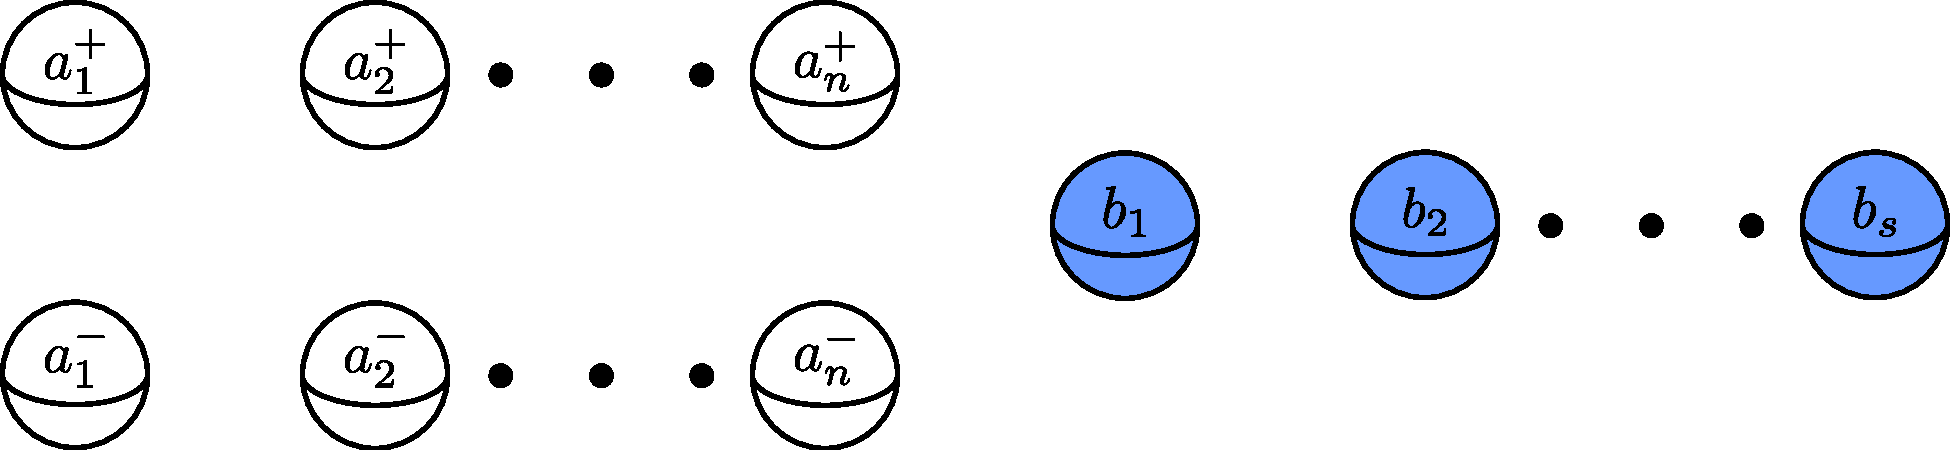
\includegraphics[width=\textwidth]{figures/spherestoglue.pdf}
  \caption{The manifold $M_{n,p}$ can be contained from  $S^3$
  by deleting the interior of $2n+p$ balls then identifying
  $n$ pairs of spheres via the antipodal map.}
  \label{fig:sphereglue}
\end{figure}


With this model of $\oout F_n$
the analog of the curve complex is the complex of embedded spheres in $M_n$.
Let $\mathcal S_{n,p}$
be the complex of spheres in $M_{n,p}$.
The vertices of $\mathcal S_{n,p}$ are
homotopy classes of essential, embedded 2-spheres $S^2 \hookrightarrow M_{n,s}$ in $\mathcal S_{n,p}$.
We will abuse notation and say \emph{sphere} to mean both a particular embedding $S^2\hookrightarrow M_{n,p}$
and its homotopy class, as dictated by context.
A set of spheres forms a simplex if there are mutually disjoint embeddings of the homotopy classes.
Hatcher showed that
the realization of $\mathcal S_{n}$
contains a dense subspace homeomorphic to Culler-Vogtmann outer space \cite{MR1314940}.
Aramayona and Souto showed that the sphere complex itself is
a combinatorial model for $\oout F_n$ \cite{souto}.

\begin{restatable}{theorem}{aramsouto}
\label{aramsouto}
The natural map $\oout F_n \to \aaut \mathcal S_n $ is an isomorphism for $n\geq 3$.
\end{restatable}

\begin{figure}[h!]
  \centering
  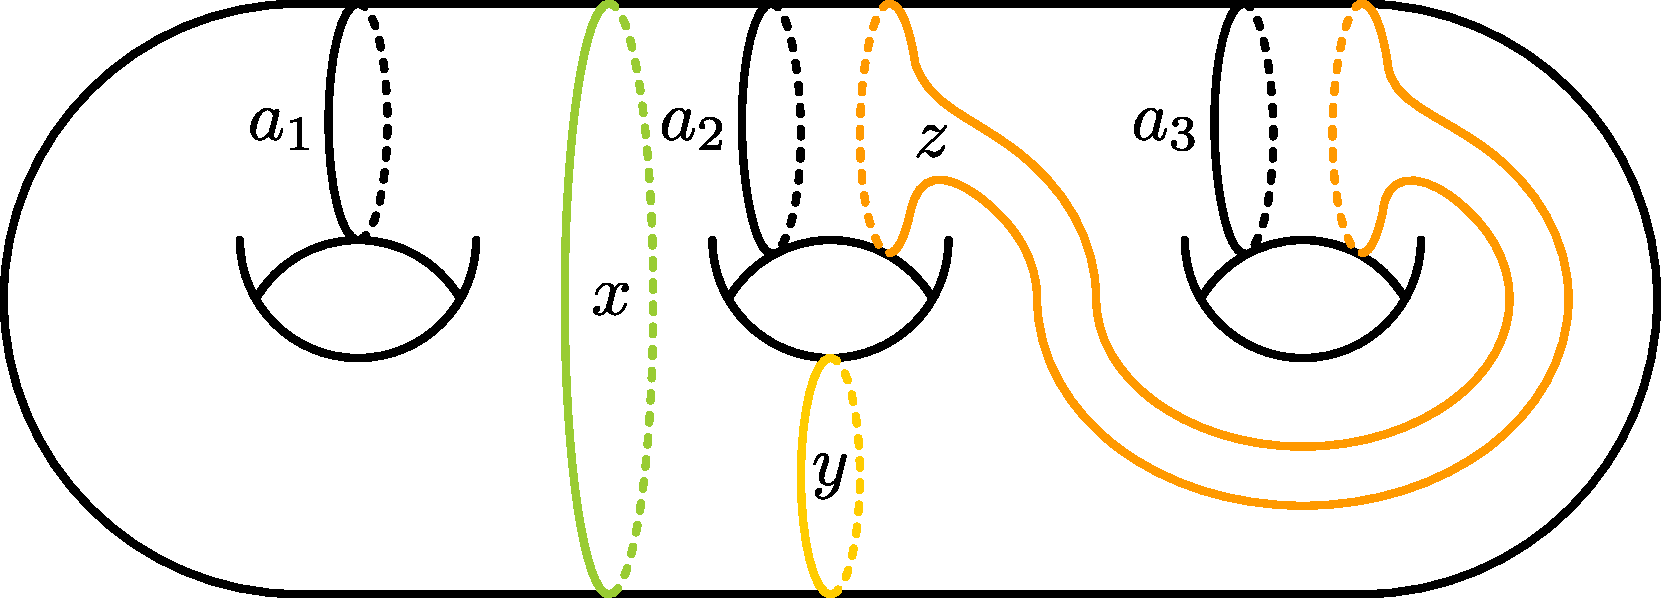
\includegraphics[width=.7\textwidth]{figures/samplecurves.pdf}
  \caption{
  A maximal collection of disjoint curves bounding disks in the handlebody.
  The prescribed doubling gives spheres of $M_3$
  specifying a maximal simplex of the sphere complex $\mathcal S_3$.
  }
  \label{fig:samplecurves}
\end{figure}

\begin{figure}[h!]
  \centering
  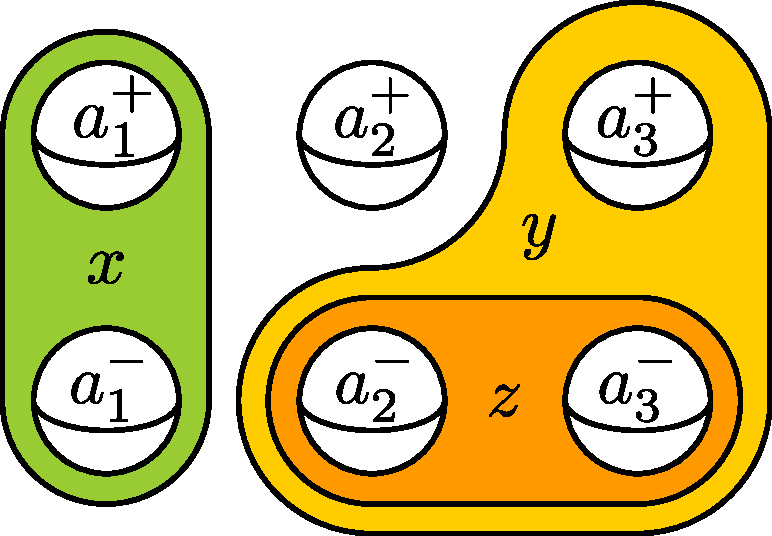
\includegraphics[width=.3\textwidth]{figures/samplespheres.pdf}
  \caption{
  A maximal collection of disjoint spheres of $S^3$ with spheres removed.
  The prescribed gluing gives spheres of $M_3$
  specifying a maximal simplex of the sphere complex $\mathcal S_n$.
  }
  \label{fig:samplespheres}
\end{figure}

There are two helpful diagramatic approaches to considering
spheres in $M_{n}$, shown in Figures \ref{fig:samplecurves} and \ref{fig:samplespheres}.
The first represents a sphere by  considering
a disk-bounding curve in a genus $n$ handlebody $H_n$,
$$x: (D^2,S^1) \hookrightarrow (H_n, S_n).$$
Then $x$ induces an embedding $x:S^2 \hookrightarrow M_n$
by taking two copies of $H_n$ and identifying the boundary
$\partial H_n = S_n$ of the two copies
$$
\begin{tikzcd}
  (D^2,S^1) \arrow[r] \arrow[d] &
  D^2 \sqcup_{S^1} D^2 \arrow[r] \arrow[d] &
  S^2 \arrow[d]  \\
  (H_n,S_n) \arrow[r]&
  H_n \sqcup_{S_n} H_n \arrow[r] &
  M_n.
\end{tikzcd}
$$
This gives a surjection from homotopy classes
of $(D^2,S^1)$ in $(H_n,S_n)$ to homotopy classes of $S^2$ in $M_n$,
but this representation by disks is not unique.
As in Figure \ref{fig:spheredisk}, Dehn twists about disk bounding curves intersecting $x$ give
distinct disks that glue up to give homotopic spheres in $M_n$.
The punctured manifold $M_{n,p}$ is similarly obtained by gluing a handlebody with $p$ half balls removed along the surface $S^p_n$.

\begin{figure}[h!]
  \centering
  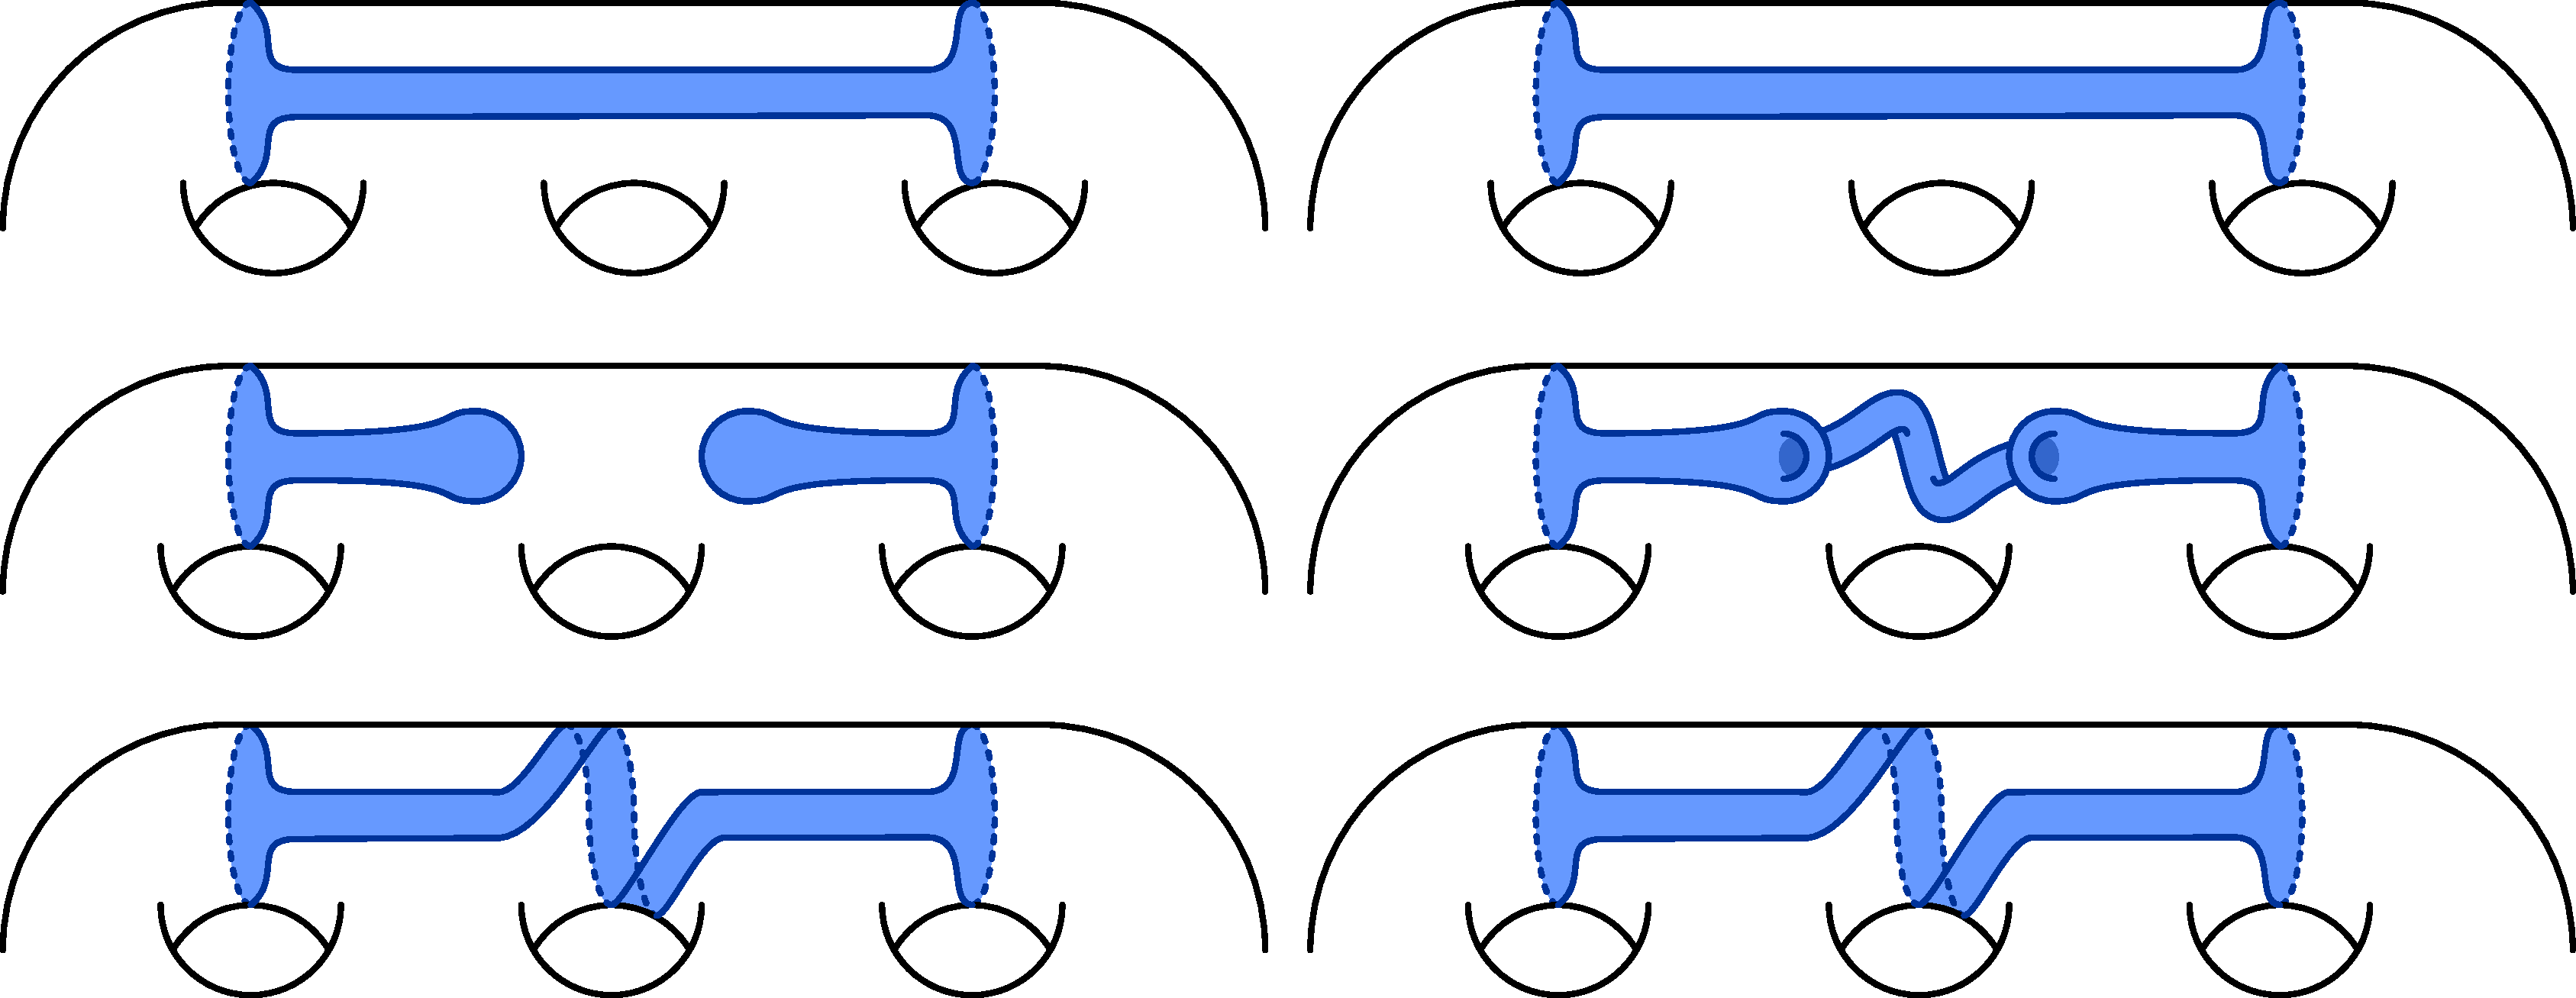
\includegraphics[width=\textwidth]{figures/spheredisk.pdf}
  \caption{
   Identifying the two copies of a handlebody along their boundary obtains $M_n$ and glues disks into spheres. Disks differing by Dehn twists about curves bounding disks in the handlebody glue to the same sphere.
  }
  \label{fig:spheredisk}
\end{figure}

A second diagramatic representation is to consider cutting
$M_{n,p}$ along a collection of $n$ disjoint nonsepating spheres
to obtain $S^3$ with $2n+p$ open balls removed.
Label the resulting boundary $S^2$ spheres
$x^+_{a_1},\ldots,x^+_{a_n}$
and
$x^-_{a_1},\ldots,x^-_{a_n}$
and
$x_{b_1},\ldots,x_{b_p}$.
Then identifying $x^+_{a_i}$ and $x^-_{a_i}$ via the $S^2$ antipodal map obtains $M_{n,p}$ again.
Then for any basepoint $q \in M_{n,p}$
we have a basis for $F_n \cong \pi_1(M_{n,p},q)$
as $a_1, \ldots, a_n$
with $a_i$ the loop disjoint from $x_{a_j}$ for $j \neq i$
and intersecting $x_{a_i}$ once by traveling into
$x^+_{a_i}$
and out of
$x^-_{a_i}$, which we defined to be positive intersection.
Diffeomorphisms of $M_n,p$ realizing $\oout_{n,p}$
can be described using this model.
By capping every boundary component of
$M_{n,p}$ with a copy of $M_{1,1}$
we can include
 $\oout_{n,p} \hookrightarrow \oout F_{n+p}$
and consider diffeomorphisms of $M_{n+p,0}$
that preserve (setwise and with orientation) the set of separating spheres
where we glued the capping $M_{1,1}$ and the nonseparating spheres contained inside.

\begin{enumerate}
  \item Permutations $\sigma$ of $\{a_1,\ldots,a_n\}$ can be realized by any
  diffeomorphism sending sphere $x_{a_i}$ to $x_{\sigma(a_i)}$
  \item Inversion $\iota_1: a_1 \mapsto a_1^{-1}$
  can be realized by cutting $M_n$ along $x_{a_1}$
  exchanging the spheres $x^+_{a_1}$ and $x^-_{a_1}$
  and then regluing $x^+_{a_1}$ and $x^-_{a_1}$
  \item Transposition $\tau_{12}: a_1 \mapsto a_1a_2$
  can be realized by cutting $M_n$ along $x_{a_1}$,
  pushing $x^-_{a_1}$ along a loop that intersects $x_{a_2}$
  once negatively and disjoint from $x_{a_i}$ with $i\neq 1,2$,
  and finally regluing $x^+_{a_1}$ and $x^-_{a_1}$
  We will also refer to this as the push of $x^-_{a_1}$ through $x^-_{a_2}$.
  See Figure \ref{fig:transvect}.
  \item Conjugation $\eta: a_1 \mapsto a_1b_1a_1^{-1}$
  can be realized by  pushing $x_{b_1}$ along a loop that intersects $x_{a_1}$ once negatively and is disjoint from $x_{a_i}$ for $i \neq 1$
\end{enumerate}

\begin{figure}[h!]
  \centering
  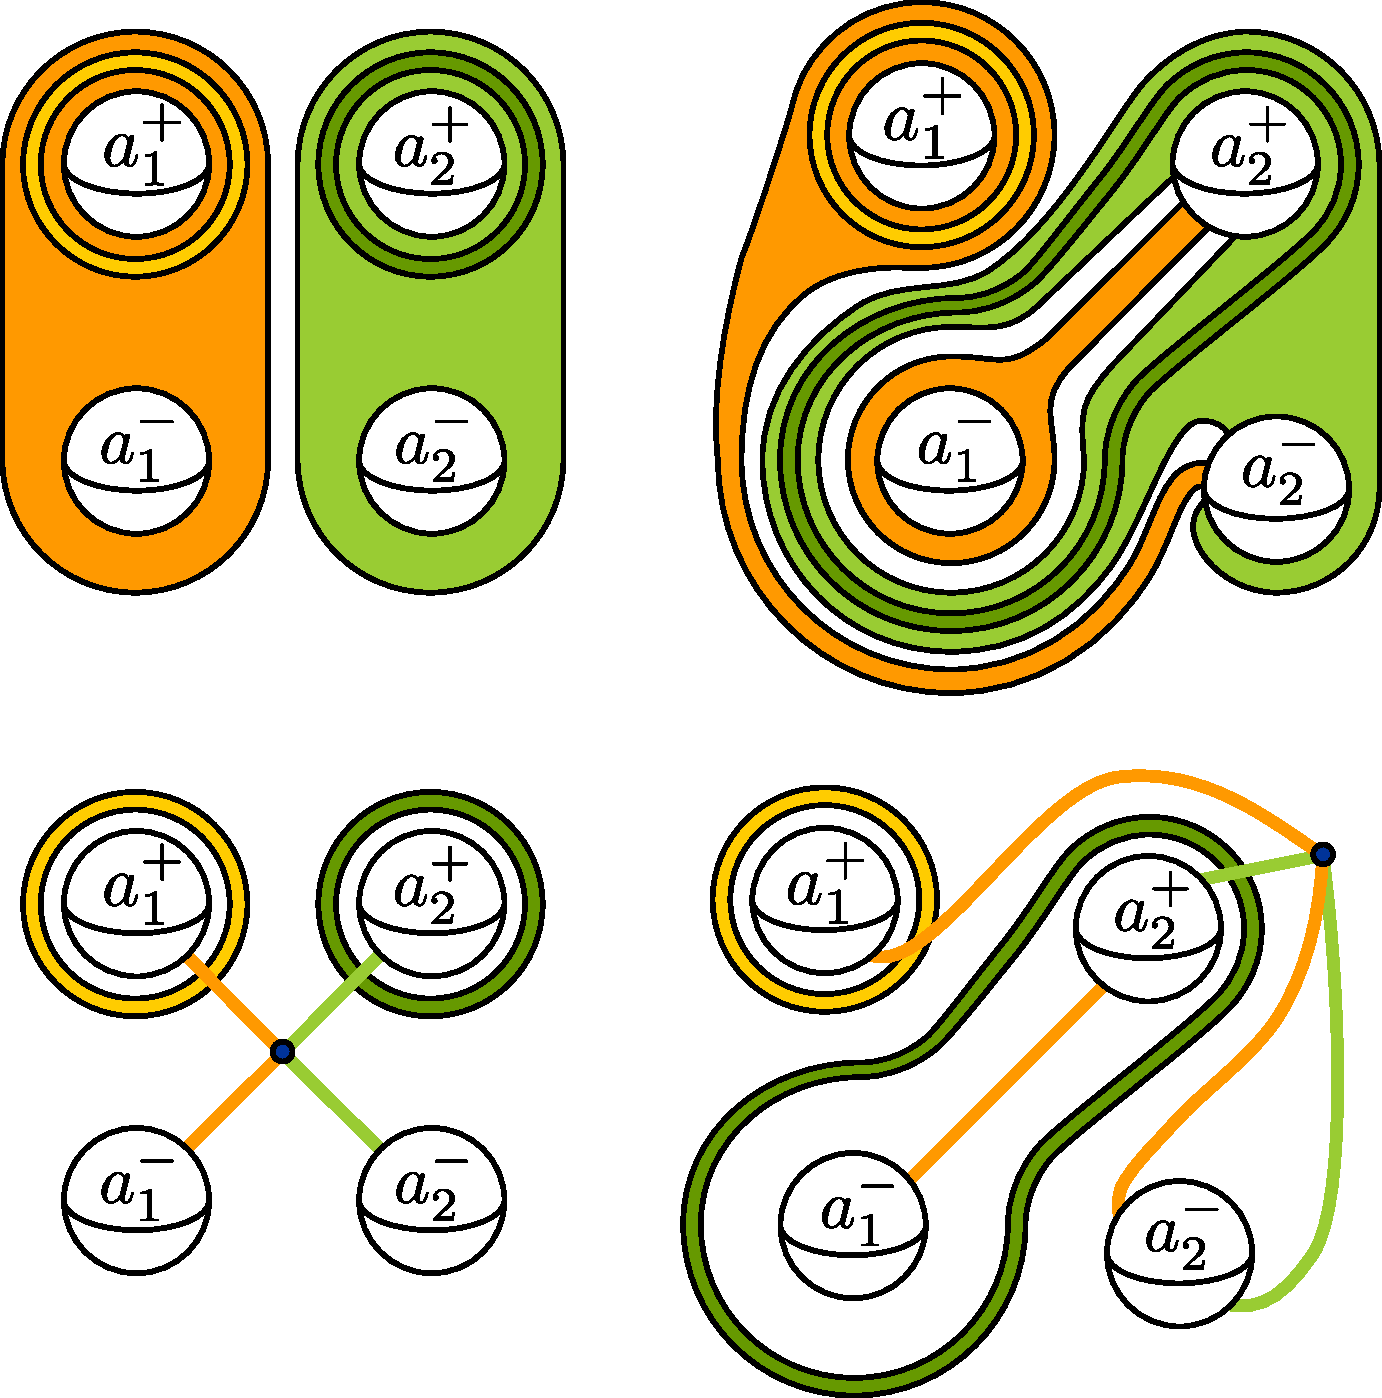
\includegraphics[width=.6\textwidth]{figures/transvect.pdf}
  \caption{
  Pushing $x^-_{a_1}$ through $x^-_{a_2}$ induces the transvection $a_1 \mapsto a_1a_2$ on the fundamental group $\pi_1$.
  }
  \label{fig:transvect}
\end{figure}


By homotoping a sphere so that it is based at $q$,
we obtain a splitting of $\pi_1(M_n,q) \cong F_n$,
and in fact conjugancy classes of splittings of $F_n$ are in bijection with spheres of $M_n$.
By considering these splittings,
Handel and Mosher show that $\mathcal S_{n}$
is $\delta$-hyperbolic \cite{MR3073931}.



In \cite{MR1314940} Hatcher shows $\mathcal S_n$ is contractible and describes
a normal form for spheres embedded in $M_n$.
A maximal collection $\Sigma$ of disjoint spheres has $3n-3$ spheres. (One could, for example take the disks of a pants decomposition in the handlebody.)
Cutting $M_n$
along $\Sigma$ such a collection of spheres
produces $2n-2$ copies of $M_{0,3}$.
Hatcher shows that any sphere $x$ of $M_{n}$
can be homotoped so that $x$ is parallel to a sphere of
$\Sigma$ or meets them tranversely in a nonempty
colleciton of circles splitting $x$
into components $x_i$ such that
\begin{enumerate}
  \item Each component $x_i$ meets any sphere of $\Sigma$ in at most one circle.
  \item No component $x_i$ is a disk isotopic by an isotopy fixing its boundary to a disk in a sphere of $\Sigma$
\end{enumerate}
Further the homotopy class of $x$ is uniquely determined by the data of the components $x$ as a sphere parallel to a sphere of $\Sigma$, or else the components $x_i$ as a disk, annulus, or pair of pants in each component of $M_n$ cut along $\Sigma$, and the spheres of $\Sigma$ that $x_i$ boundary components intersect.

\begin{figure}[h!]
  \centering
  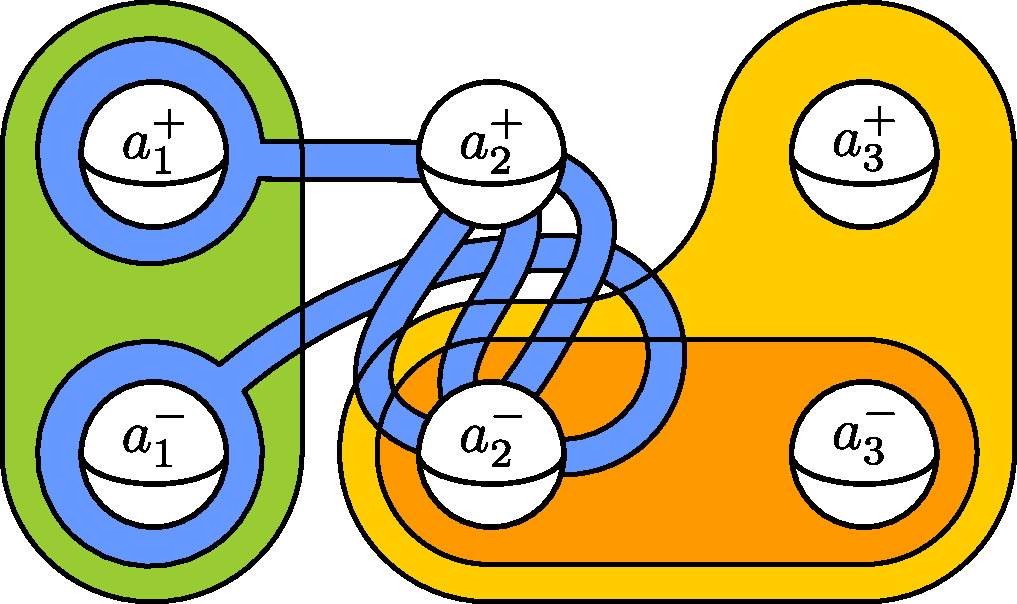
\includegraphics[width=.6\textwidth]{figures/normalform.pdf}
  \caption{
   The sphere for the splitting $\left \langle a_1^{-1}a_2^4 \right \rangle \ast \left \langle a_2,a_3 \right \rangle$ in Hatcher normal form with respect to the maximal collection $\{a_1,a_2,a_3,x,y,z\}$ in $M_3$.
  }
  \label{fig:normalform}
\end{figure}

Just as in the case of curves of the surface,
the spheres of a surface have a
{change of coordinates principle}:
spheres $x$ and $y$ lie in the same $\oout_{n,p}$ orbit if
and only if their complements in $M_{n,p}$ are homeomorphic.
Thus the topological types of spheres are
\emph{nonsepararing}, and \emph{separating} spheres whose complement is $M_{n'p'} \sqcup M_{n'',p''}$
where
$n=n'+n''$ and $p+2=p'+p''$.
For a separating sphere $x$
we refer to the connected components of its complement as the \emph{sides}
of $x$, and the \emph{small side} as whichever has a less negative Euler characteristic.
We refer to a sphere $y$ on the small side of $x$ as \emph{engulfed} by $x$,
or \emph{engulfed} if it lies on the large side of $x$.

Pandit has shown that the nonseparating spheres
also constitute a combinatorial model for $\oout F_n$ \cite{pandit}.
That is let $\nosep  \subset \mathcal S_n$ be the induced subcomplex spanned by nonseparating spheres. Pandit gives
\begin{theorem}
  For $n \geq 3$ the natural map
  $$\outn \to \Aut{\nosep}$$
  is an isomorphism.
\end{theorem}


% !TEX root = thesis.tex
\chapter{Birman Point Pushing}
\label{chap:birman}

In this chapter we consider the
relationship of combinatorial models
after adding or deleting punctures.
We will see in Section \ref{sect:curvepunc}
how the Birman exact sequence
appears in the automorphisms of the curve complex.
Section \ref{sect:spherepunc}
follows a parallel outline to show that adding
punctures to $M_{n,p}$ creates an analogous fibration
of the sphere complex.


We recall the Theorem \ref{thm:curvecomplex}
of
Ivanov \cite{MR1460387},
Korkmaz \cite{MR1696431},
and
Luo \cite{MR1722024}.

\curvecomplex*

Although their methods of proof are general and
do not require separate consideration of the closed and
punctured cases, we will demonstrate
that additional punctures of the surface
leave the isomorphism
$
\mcg^\pm S_{g,p} \to  \aaut \mathcal C S_{g,p}
$
intact.
We do so by attempting to substitute this ismorphism into the Birman exact sequence.
Recall Birman's Theorem \ref{thm:birman}

\birman*



\section{Curves and Punctures}
\label{sect:curvepunc}
Our goal in this section will be an independent proof of
the following
weaker version of Theorem \ref{thm:curvecomplex},
in preparation for the free group analog in Section \ref{sect:spherepunc}.
% The proof is structured as follows:
% \begin{enumerate}
%   \item We first show that the topological type of curves is preserved by automorphisms of $\mathcal C S_{g,p}$
%
% \end{enumerate}


% \begin{restatable}{theorem}{curvecomplex}
%   The natural map
%   $$
%   \mcg^\pm S_{g,p} \to  \aaut \mathcal C S_{g,p}
%   $$
%   is an isomorphism whenever the curve complex
%   $\mathcal C S_{g,p}$
%   has positive dimension $3g+p-4$ and $(g,p) \neq (1,2)$.
%   \label{thm:curvecomplex}
% \end{restatable}

% \begin{restatable}{theorem}{thmaddpunc}
%   If the natural map
%   $$
%   \mcg^\pm S_{g,p} \to  \aaut \mathcal C S_{g,p}
%   $$
%   is an isomorphism, then so is
%   $$
%   \mcg^\pm S_{g,p+1} \to  \aaut \mathcal C S_{g,p+1}.
%   $$
%   \label{thm:addpunc}
% \end{restatable}

\thmaddpunc*

% The proofs of Theorems \ref{thm:addpunc} and  \ref{thm:puncrigid}


\begin{remark}
Every simplex $\Delta$ of $\mathcal C S_{g,p}$
is a collection of disjoint curves that cuts up the surface $S_{g,p}$ into
a number of connected components.
This gives a
Bass-Serre
graph of groups
% \cite{MR607504}
for $\pi_1 S_{g,p}$
induced by the $\Delta$ specified splitting.
The underlying simple graph
is the adjacency graph studied in
Margalit, Behrstock \cite{MR2239449}
and Shackleton \cite{MR2318453}.
These also appear as graphs associated to
pants decompositions in \cite{MR579573}.
\end{remark}

\begin{definition}
Let $\Delta \subset \mathcal C S_{g,p}$ be a simplex.
The \emph{region adjacency graph} $\mathcal G_\Delta$
of $\Delta$
is the graph whose
vertices are the connected components of
the cut surface
$$
S_{g,p} - \bigcup_{c \in \Delta} c
$$
with an edge for
every curve $c$ incident to the regions it bounds.

We will also consider the graph simplification
$\mathcal G^{simp}_{\Delta}$ obtained
from the (possibly looped, multi-edged) graph
$\mathcal G_\Delta$ by
removing any self-loops and
identifying multi-edges.
\label{def:graphadj}
\end{definition}

Automorphisms
of the curve complex act naturally on the
set of adjacency graphs by isomorphism.
Similar Lemmas are due to Margalit and Behrstock \cite{MR2239449},
though the graphs considered are simple graphs without multiedges or loops.

\begin{lemma}
  Curve complex automorphisms preserve the
  edge incidence of region adjacency graphs.

  Let $\phi \in \aaut \mathcal C S_{g,p}$
  and let $\Delta$ be a simplex of $\mathcal C S_{g,p}$
  with adjacency graph $\mathcal G_\Delta$.
  Then $e_c,e_{c'}$ are incident edges of $\mathcal G_\Delta$
  if and only if $e_{\phi(c)},e_{\phi(c')}$
  are incident edges of $\mathcal G_{\phi(\Delta)}$.
  \label{lemma:adjgraph}
\end{lemma}

\begin{proof}
  We will argue that $\phi$ induces a bijection
  $\phi_\ast : E_{\mathcal G_\Delta} \to E_{\mathcal G_{\phi(\Delta)}}$
  on the set of edges
  that preserves the incidence
  and non-incidence of edges.

  Let $e_c$ be an edge of $\mathcal G_\Delta$ given by curve $c$.
  Then $\phi_\ast (e_c) = e_{\phi(c)}$  defines a bijection
  between the edges of $\mathcal G_\Delta$ and $\mathcal G_{\phi(\Delta)}$.
  We will show $e_c$ is incident to $e_{c'}$ if
  and only if there is a curve of $\mathcal C S_{g,n}$
  intersecting $c$ and $c'$, but no other curve of $\Delta$.
  Then $e_{\phi(c)}$ is incident to $e_{\phi(c')}$
  if and only if there is a curve of $\mathcal C S_{g,n}$
  intersecting $\phi(c)$ and $\phi(c')$, but no other curve of $\phi(\Delta)$.

  Suppose $e_c$ is incident to $e_{c'}$.
  Observe every region  of
  $
  S_{g,p} - \bigcup_{c \in \Delta} c
  $
  contains an embedded pair of pants $S_{0,3}$.
  So if we consider regluing regions along $c$ and $c'$,
  we obtain the
  component $R$ of $
  S_{g,p} - \bigcup_{b\neq c,c'} b
  $
  with $c,c' \subset R$.
  Then $R$ must contain an embedded $S_{0,5}$
  or an $S_{1,1}$.
  So $R$ contains a curve $c''$ intersecting $c$ and $c'$,
  and since $c'' \subset R$, it does not intersect any other curve of $\Delta$.

  Suppose $e_c$ is not incident to $e_{c'}$ in $\mathcal G_{\Delta}$.
  Then there is a multicurve $\Delta' \subset \Delta$
  that separates $c$ from $c'$ in $S_{g,p}$.
  But then every curve that intersects $c$ and $c'$ must intersect a curve of $\Delta'$.
\end{proof}

\begin{example}
  Edge incidence preservation is not always enough to guarantee a graph isomorphism.


Recall the Whitney Graph Isomorphism Theorem \ref{thm:whitney}
states that for simple graphs an edge bijection preserving incidence is an isomorphism,
except in the case of $K_3$.
However, for non-simple graphs, edge incidence can be preserved by swapping a loop with a multiedge.
\begin{figure}[h!]
  \centering
  
\includegraphics[width=.15\textwidth]{figures/graphexamples2.pdf}
  \caption{An edge bijection preserving incidence may not be an isomorphism for multigraphs.
  A self-loop might swap with a multiedge if the multiedge is not incident to additional edges.}
  \label{fig:looptomultiedge}
\end{figure}
This is the case for some automorphisms  of $\mathcal C S_{1,2}$ acting on region adjacency graphs.
Luo describes how a quotienting of  $S_{1,2}$ by a hyperelliptic involution gives
an isomorphism $\aaut \mathcal C S_{1,2} \to \aaut \mathcal C S_{0,5}$ \cite{MR1722024}.
An automorphism of $\mathcal C S_{1,2}$ bijects edges and preserves incidence of the region adjacency graph, but may not induce an isomorphism. The corresponding automorphism of $\mathcal C S_{0,5}$ induces an
isomorphism of the region adjacency graph, as in Figure \ref{fig:s12ands03}.




\begin{figure}[h!]
  \centering
  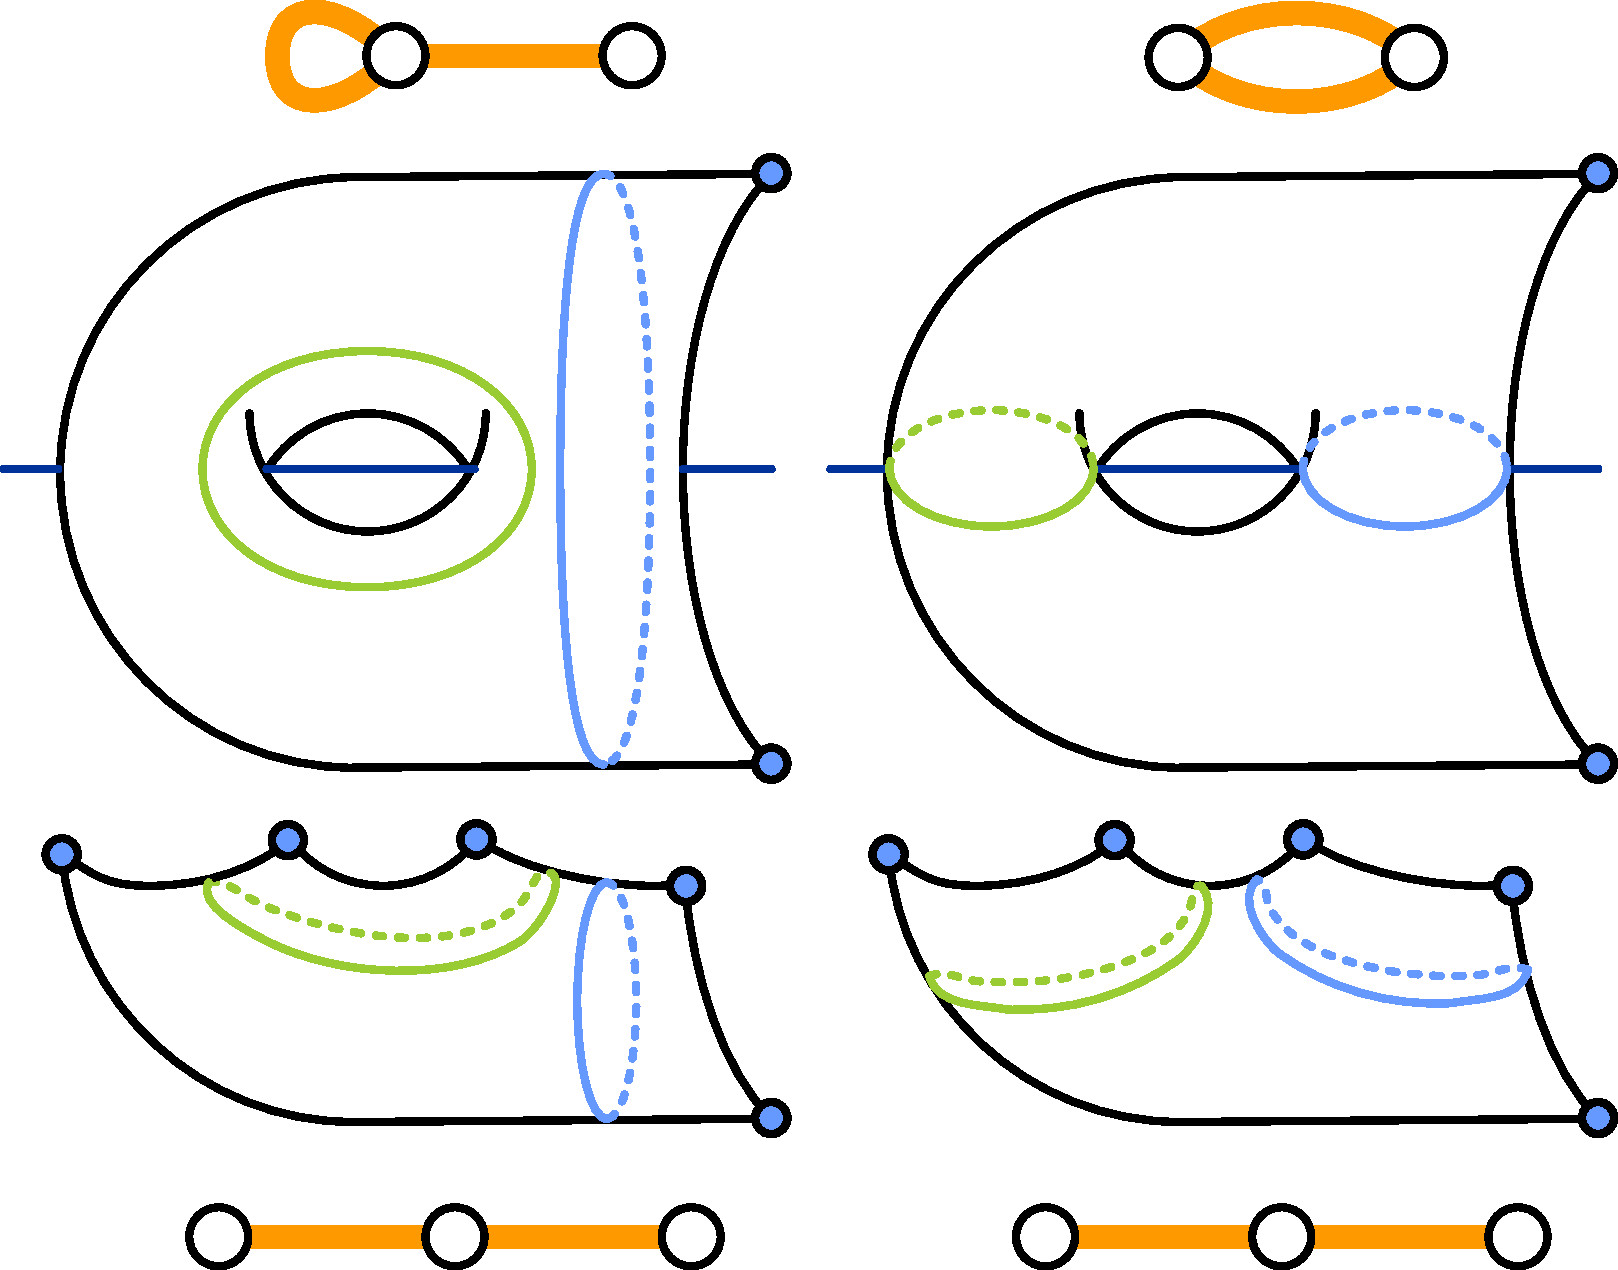
\includegraphics[width=.7\textwidth]{figures/s12ands03.pdf}
  \caption{(Top) Two nonisomorphic region adjacency graphs can be exchanged by an automorphism of $\mathcal C_{1,2}$,
  though the edge incidence relation is preserved.
  (Bottom)
  Such an automorphism of $\mathcal C S_{1,2}$ corresponds via hyperelliptic involution to a homeomorphism of $S_{0,5}$.}
  % An automorphism of $\mathcal C S_{1,2}$ bijects edges and preserves incidence of the region adjacency graph, but may not induce an isomorphism. The corresponding automorphism of $\mathcal C S_{0,5}$ induces an isomorphism of the region adjacency graph.}
  \label{fig:s12ands03}
\end{figure}

\end{example}



\begin{corollary}
  Curve complex automorphisms induce isomorphisms of
  region adjacency graphs of maximal simplices.

  Suppose that $3g+p\geq 5$  and $(g,p)\neq(1,2)$.
  Let $\phi \in \aaut \mathcal C S_{g,p}$
  and let $\Delta$ be a maximal simplex of $\mathcal C S_{g,p}$.
  Then $\mathcal G_\Delta$ and
  $\mathcal G_{\phi(\Delta)}$
  are isomorphic graphs.
  \label{cor:adjgraph}
\end{corollary}

\begin{proof}
  Any maximum simplex $\Delta$
  gives a pants decomposition of the surface $S_{g,p}$
  with $3g+p-3$ curves and $2g+p-2$ pairs of pants.
  So $\mathcal G^{simp}_\Delta$
  and
  $\mathcal G^{simp}_{\phi(\Delta)}$
  are simple, connected graphs with the same number of
  vertices and the same edge-incidence relations.
  Then by Whitney's Theorem \ref{thm:whitney},
  $\mathcal G^{simp}_\Delta$ is isomorphic to
  $\mathcal G^{simp}_{\phi(\Delta)}$.

  To see that self-loops are preserved, observe
  that as $\Delta$ cuts $S_{g,p}$ into pairs of pants,
  every vertex of $\mathcal G_\Delta$ has degree at most 3.
  Then if $e_c$ is a self-loop at vertex $v_R$,
  it is incident to exactly one other edge $e_x$
  that cannot be a self-loop, so $e_x$ is uniquely represented in $\mathcal G^{simp}_\Delta$.
  If $(g,p) \neq (1,2)$, then $e_x$ is incident to another edge $e_y$.
  Then $e_\phi(x)$ is
  also uniquely represented in the isomorphic graph $\mathcal G^{simp}_\Delta$
  and has a degree 1 vertex.
  Then in $\mathcal G^{simp}_\Delta$, $e_\phi(x)$
  is incident to $e_\phi(y)$, and $e_\phi(c)$ is incident to $e_\phi(x)$,
  but not $e_\phi(y)$ or any other edge, so $e_\phi(c)$   must be a loop at the vertex
  that is degree 1 in $\mathcal G^{simp}_{\phi(\Delta)}$.
\end{proof}


\begin{lemma}
  Automorphisms of the curve complex preserve the sides and topological type of curves.

  Suppose that $3g+p \geq 5$ and $(g,p)\neq(1,2)$.
  Let $\phi \in \aaut \mathcal C S_{g,p}$ and let $x$ be a curve.
  Then there is a homeomorphism of $S_{g,p}$ exchanging $x$ and $\phi(x)$.
  Furthermore, if $x$ is separating and $y,y'$ lie on the same side of $x$,
  then $\phi(y),\phi(y')$ lie on the same side of $\phi(x)$.
  \label{lemma:curvetype}
\end{lemma}
\begin{proof}
  We will characterize each topological type of curve
  by a combinatorial property of a corresponding region adjacency graph,
  and apply Lemmas
  \ref{lemma:adjgraph} and \ref{cor:adjgraph}.

  \begin{enumerate}[$\cdot$]
    \item Nonseparating curves:
    Observe that a curve $c$ is nonseparating if and only if
    there is a maximal simplex $\Delta$ such that $e_c$
    is a self-loop in the region adjacency graph $\mathcal G_\Delta$.
    \item Separating curves:
    Observe that if curve $x$ separates $S_{g,p}$
    $$
    S_{g,p} = S_{g',p'} \sqcup_c S_{g-g',p-p'+2}
    $$
    then the corresponding edge $e_x$ of the
    region adjacency graph
    $\mathcal G_\Delta$
    is a cut edge.
    More specifically, if
    $$\Delta = \Delta_+ \cup \{x\} \cup \Delta_-$$
    with $\Delta_+$ and $\Delta_-$
    the curves on each side of the separating curve $c$,
    then $e_x$ separates $\mathcal G_\Delta$
    $$\mathcal G_\Delta  - \{e_x\}  = \mathcal G_{\Delta_+} \sqcup  \mathcal G_{\Delta_-}$$
    into the components
    $\mathcal G_{\Delta_+}$, with
    $3g'+p'-3$ edges and genus $g'$,
    and $\mathcal G_{\Delta_-}$ with $3(g-g')+p-p'-1$ edges and genus $g-g'$.
  \end{enumerate}
  \end{proof}




\begin{remark}
For the closed surface $S_g$ the inclusion $S_{g}-\{q\} \hookrightarrow S_{g}$
induces a well defined puncture-forgetting projection map
$$
\rho_q: \mathcal C S_{g,1} \to \mathcal C S_g.
$$
by sending curves to their image.
Since we do not allow peripheral curves in $\mathcal C S_{g,1}$, no curve becomes nullhomotopic.
However, in the case of multiple punctures $P$,
the surface $S_{g,p}$ has curves bounding twice-punctured disks,
that may become peripheral if a puncture is forgotten.
Excluding these curves
gives a subcomplex $\mathcal C(S_{g,p},q) \subset \mathcal C S_{g,p}$
where the puncture-forgetting map is well-defined for puncture $q$.
$$
\rho_q: \mathcal C(S_{g,p},q) \to \mathcal C S_{g,p-1}
$$

Kent, Leininger, and Schleimer \cite{MR2599078}
show that this forgetful projection has
fibers described by Bass-Serre trees of the surface fundamental group
so that there is a fibration of the form
$$
\mathcal T \to \mathcal C(S_{g,p},q) \to \mathcal C S_{g,p-1}.
$$
More rigorously,
\end{remark}

\begin{theorem}
  Let $\Delta \subset \mathcal C S_{g,p}$
  be a simplex with interior point $x \in \Delta$.
  Then the fiber $\rho^{-1}_q(x)$ is
  $\pi_1 \left ( S_{g,p}, q \right )$-equivariantly
  homeomorphic to the tree $\mathcal T_\Delta$,
  the Bass-Serre tree for the splitting of
  $\pi_1 \left ( S_{g,p}, q \right )$
  determined by the multicurve $\Delta$.
  \label{thm:kent}
\end{theorem}

\begin{remark}
Observe that $\mathcal C(S_{g,p},q)$
is not characteristic in $C S_{g,p}$,
since in general automorphisms of $C S_{g,p}$ will permute the punctures.
Let $\aaut (\mathcal C S_{g,p},q) < \aaut \mathcal C S_{g,p}$
be the subgroup of $\aaut \mathcal C S_{g,p}$
that preserves the fibration
$\mathcal C(S_{g,p},q) \to \mathcal C S_{g,p-1}$, that is
$$\phi \left ( \rho_q^{-1}\rho_q(x) \right ) = \rho_q^{-1}\rho_q(\phi(x))$$
for every $x \in C(S_{g,p},q)$.

If $\phi \in \aaut \mathcal C(S_{g,p},q)$ then there is a well defined push-forward
automorphism of the less-punctured quotient $\mathcal CS_{g,p-1}$.
Define $\rho^\ast_q \phi \in \aaut \mathcal CS_{g,p-1}$
by
$$\left (  \rho^\ast_q \phi \right ) (x) = \rho_q \left(\phi (y) \right )$$
for any choice of $y \in \rho^{-1}_q(x)$. This is well defined since if $y' \in \rho^{-1}_q(x) =\rho^{-1}_q\rho_q(y)$
then
$$\phi(y') \in \phi(\rho^{-1}_q \rho_q y ) = \rho^{-1}_q \rho_q\phi( y )$$
by definition of $\aaut \mathcal C(S_{g,p},q)$.
Then this gives a pushforward map
$$
\rho_q^\ast : \aaut \mathcal (CS_{g,p},q) \to  \aaut \mathcal CS_{g,p-1}
$$
given by $\phi \mapsto \rho_q^\ast \phi$ as above.
\end{remark}

These automorphisms display the structure of the Birman exact sequence.

\begin{lemma}
  This diagram commutes
  $$
  \begin{tikzcd}
  1 \arrow[r]&
  \pi_1(S_{g,p-1},q) \arrow[r] \arrow[d]&
  \mcg^{\pm}(S_{g,p},q)  \arrow{r}{f_q} \arrow[d]&
  \mcg^{\pm}S_{g,p-1} \arrow[r] \arrow[d]&
  1 \\
  1 \arrow[r]&
  \pi_1(S_{g,p-1},q) \arrow{r}{\alpha}&
  \aaut \mathcal C (S_{g,p},q)  \arrow{r}{\rho^\ast_{q}}&
  \aaut \mathcal C S_{g,p-1} \arrow{r}&
  1 \\
  \end{tikzcd}
  $$
  and has exact rows when $\rho_{q}$ is surjective.
  \label{lemma:exact}
\end{lemma}



\begin{proof}
  The pushforward $\rho^\ast_q: \aaut \mathcal C (S_{g,p},q)  \to
  \aaut \mathcal C S_{g,p-1}$
  is defined by
  $$
  (\rho^\ast_q \phi) (x) = \rho_q( \phi(y))
  $$
  where $y \in \rho^{-1}_q(x)$. This is well defined since if $z \in \rho^{-1}_q(x)$
  then $\phi(z))  \in \rho^{-1}_q \rho_q (\phi(y))$ by definition of $\aaut \mathcal C (S_{g,p},q)$.


  The map $\alpha$ is defined by the first square,
  so it certainly commutes.
  And $\alpha$
  gives a well defined injection,
  since for any nontrivial loop $\gamma$
  there is a nonseparating curve $c$
  that intersects $\gamma$ so that the point pushing map
  $\alpha(\gamma)$ moves $c$, and $c \in \mathcal C (S_{g,p},q)$.

  The second square must commute,
  since if $[\psi] \in \mcg^\pm (S_{g,p},q)$
  is a mapping class and $c$ a curve of $S_{g,p}$,
  the homotopy class of $\psi(c)$ is the same if we first
  allow homotopies of the homeomorphism $\psi$ which do not fix $q$, or if we first consider the homeomorphism $\psi$
  up to homotopy fixing $q$, then homotope the curve $\psi(c)$ forgetting $q$.

  As in  Theorem \ref{thm:kent},
  the fiber $\rho^{-1}_q(x)$ of the projection
  $\rho_q: \mathcal  C (S_{g,p},q) \to \mathcal C S_{g,p}$
  for a curve $x$
  is homeomorphic to the Bass-Serre
  tree $\mathcal T_x$ given by the splitting $x$ specifies on $\pi_1(S_{g,p},q)$.
  Then the kernel $\ker \rho_{q}$ is a
  group acting faithfully on the tree $\mathcal T_\Delta$,
  so by the
  Fundamental Theorem of Bass–Serre Theory
  \ref{thm:bassserre},
  $\ker \rho^\ast_{q}$ is isomorphic to
  the fundamental group $\pi_1$ of the
  quotient graph of groups,
  but the corresponding graph of groups is
  exactly the Van Kampen splitting of $\pi_1$ induced by $x$.
  Thus
  $$\ker \rho^\ast_{q} = \mbox{image } \alpha \cong \pi_1(S_{g,p},q)$$
  and the second row is exact.
\end{proof}

We will show that, though curve complex automorphisms might not
preserve the fibers of $\rho_q$ for any particular puncture $q$, they do permute the fibers
of the puncture-forgetting projections $(\rho_q)_{q \in P}$.
We do so by proving the unique colorability of an arc complex.
Korkmaz's proof of Theorem \ref{thm:curvecomplex}
utilizes a slightly more general arc complex
allowing peripheral arcs \cite{MR1696431} and simplices of arcs that share endpoints.

\begin{definition}
  Define the pointed arc complex
  $\mathcal A S_{g,p}$
  to be the complex of homotopy classes of embedded
  non-peripheral arcs in $S_{g,p}$ with endpoints in $P$,
  where an arc is peripheral if
  it is a separating loop based at a single puncture
  and one of its sides is a punctured monogon of $S_{g,p}$.
  Two arcs or disks are adjacent in
  $\mathcal A S_{g,p}$ if their homotopy classes
  have disjoint representatives and share no punctures as endpoints.
  \label{def:ptarc}
\end{definition}

\begin{remark}
  The pointed arc complex $\mathcal A S_{g,p}$ has as vertices
  both arcs with two distinct
  endpoints and loops based at a single puncture.
  Since loops that are disjoint are always
  based at distinct punctures,
  there is an obvious way to color (in the graph-theoretic sense)
  the vertices of
  $\mathcal A S_{g,p}$ that are loops:
  assign a color to each puncture and all the loops based at that puncture.
  The arcs with distinct endpoints
  require two colors, however.
  We make a slight generalization of
  $k$-colorings to allow a privileged set of vertices that
  that require two colors.

  Recall from Definition \ref{def:color}
  that a $k,\eta$-coloring
  assigns to each vertex $x$ a set of $\eta(x)$ colors from $k$ options
  so that adjacent vertices have disjoint color sets.
\end{remark}


%#___________________
\begin{remark}
Margalit in \cite{MR2040283} discusses the
trinion pants complex.
Pants decompositions of $S_{g,p}$ are maximal simplices of
$\mathcal C S_{g,p}$,
with two such pants decompositions giving sharing
an edge in the pants complex if they differ
by a single pair of minimally intersecting curves.
Hatcher and Thurston
demonstrated the
pants complex (which they call \emph{markings}) of a surface
is connected and simply connected
in \cite{MR579573}.
We recall their result as the following lemma.
\end{remark}

\begin{lemma}
  \label{lem:maxsimppath}
  Let $\Delta,\Delta'$ be maximal $k$-simplicies of $\mathcal C S_{g,p}$.
  Then there is a sequence $\Delta = \Delta_0, \Delta_1, \ldots, \Delta_n=\Delta'$
  of maximal simplices such that
  $\Delta_i \cap \Delta_{i+1}$ is a $k-1$ simplex
  and the curves $c_i \in \Delta_i - \Delta_{i+1}$
  and $c'_i \in \Delta_{i+1} - \Delta_i$
  are contained in a single component $R$ of
  $S_{g,p} - \bigcup_{x \in \Delta_i \cap \Delta_{i+1}} x$.
  Further,
  $c_i,c'_i$ can be chosen to intersect once if $R \cong S_{1,1}$
  and twice if $R \cong S_{0,4}$.
  \label{lemma:pantspath}
\end{lemma}

\begin{remark}
Lemma \ref{lemma:pantspath}
in particular implies that for any two maximal $k$-simplicies
$\Delta,\Delta'$ contained in a $k$-colorable subgraph of $\mathcal C S_{g,p}$
the simplex $\Delta$ forces a coloring on $\Delta'$.
Bestvina, Bromberg, and Fujiwara note bounds on the chromatic number of the curve graph $\mathcal C S_{g,p}$
in \cite{MR3415065}.
Gaster, Greene, and Vlamis further develop the theory of  in \cite{2016arXiv160801589G}, where they additionally consider colorings of
a related arc complex that contains $\mathcal A S_{g,p}$ as a proper subcomplex, albeit with many more edge relations
\end{remark}

We will show that $\mathcal A S_{g,p}$ is uniquely colorable.

%#___________________

\begin{definition}
  \label{def:nest}
Fix an ordering $\sigma:P \to \{1,\ldots,p\}$ of the punctures
and let $x$ be a curve of $S_g$.
A $\sigma$-\emph{nest} of curves parallel to $x$
is the homotopy class in $S_{g,p}$
of an embedding
$$N: S^1 \times I \hookrightarrow S_{g,p}$$
such that $N$ is a homotopic to $x$ in $S_g$ by homotopy forgetting the punctures,
and image of $S^1 \times \{{\sigma(i)-1}/{(p-1)}\}$ is a loop based at puncture $\sigma^{-1}(i)$
that we refer to as the rib $N_i$.
The nest also gives a collection of $p-1$ arcs.
The  $i^{\mbox{th}}$ \emph{vertebra} of $N$ is the arc from $\sigma^{-1}(i)$ to $\sigma^{-1}(i+1)$ and given by
$$
N \left ( \{s_0\}\times  \left [ \frac{\sigma(i)-1}{p-1}, \frac{\sigma(i+1)-1}{p-1} \right]  \right )
$$
for the basepoint $s_0 \in S^1$.
We refer to $N(s_0 \times I)$ as the \emph{spine} of $N$.
\end{definition}


\begin{figure}[h!]
  \centering
  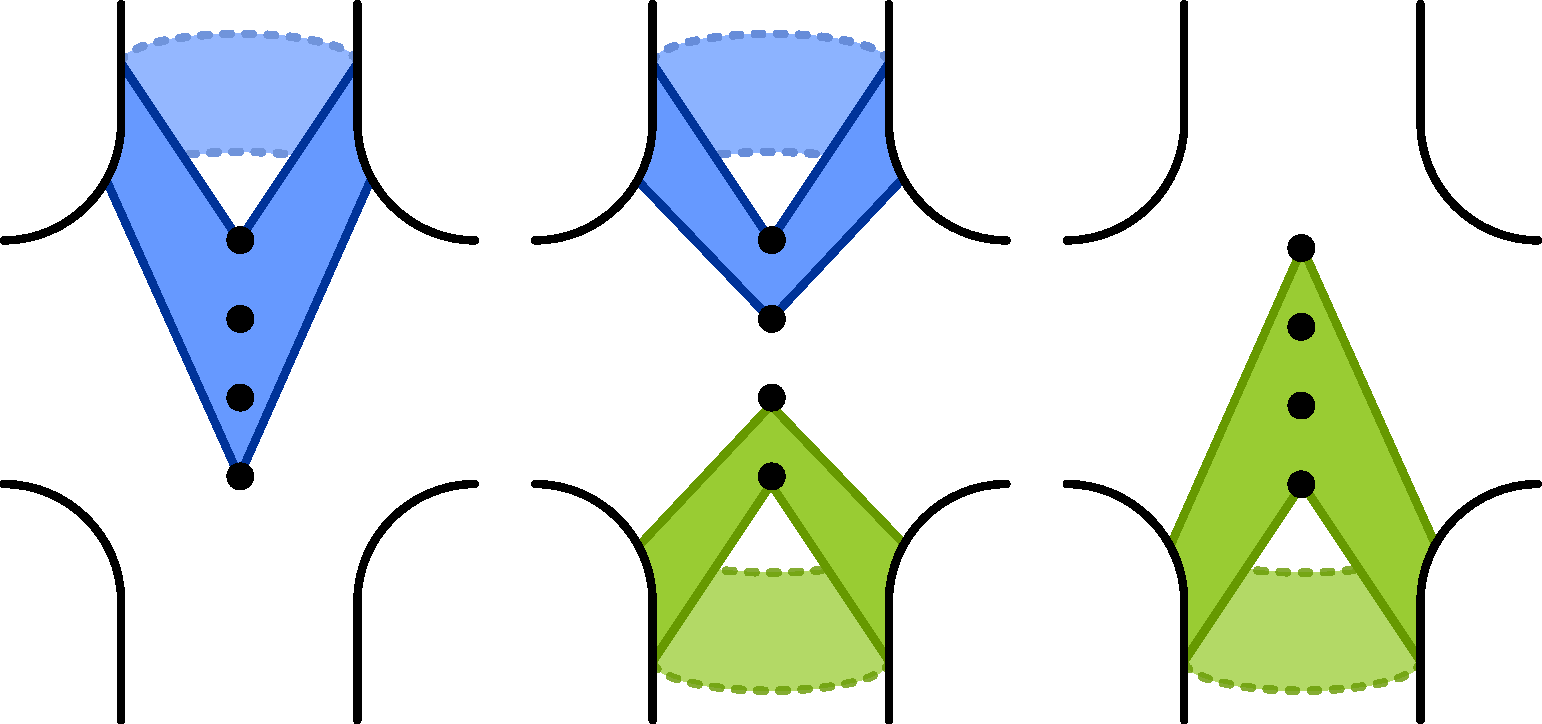
\includegraphics[width=.7\textwidth]{figures/corset.pdf}
  \caption{A color forcing path between nests parallel to disjoint curves.}
  \label{fig:corset}
\end{figure}


\begin{example}
  \label{example:nests}

  Observe that any nest $N$ in $S_{g,p}$
  specifies a maximal simplex  $\Delta_N$  in $\mathcal A S_{g,p}$.
  Further two $\sigma$-nests $N,N'$ respectively parallel to
  disjoint curves $x,x'$ of $S_{g,p}$
  specify a length $p$ sequence from $\Delta_N$ to $\Delta_{N'}$ of maximal simplices intersecting
  in codimension one faces as by replacing $N_i$ with $N'_i$, as in Figure \ref{fig:corset}.
  So $\Delta_{N}$ forces a $p$-coloring on $\Delta_{N'}$.

  \begin{figure}[h!]
    \centering
    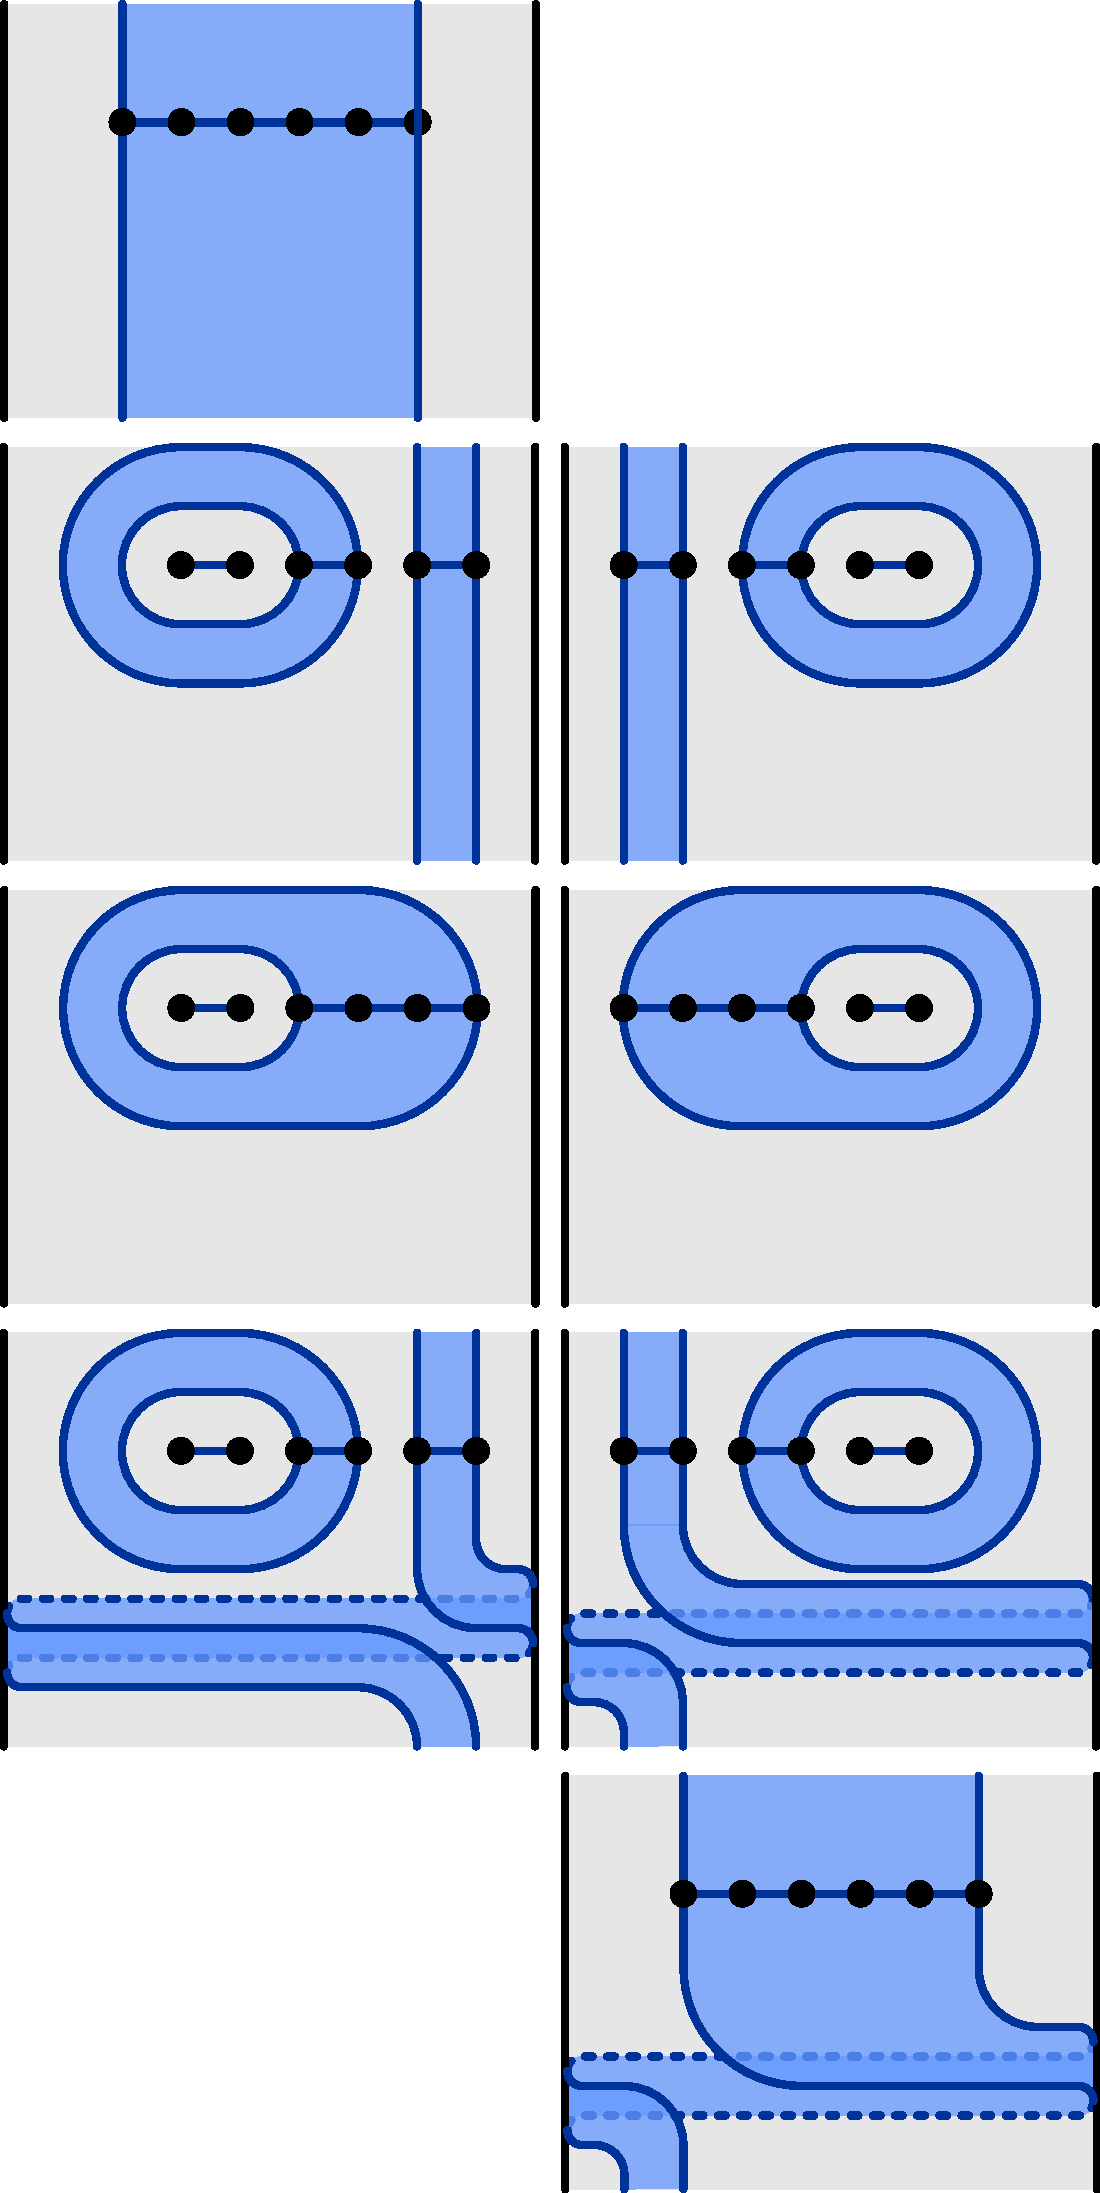
\includegraphics[width=.5\textwidth]{figures/nests.pdf}
    \caption{Two paths of simplices forcing  a coloring between nests parallel to intersecting curves.
    ``Pack'' curves on one boundary component of the nest into curves surrounding punctured disks,
    then unpack them parallel to a different curve of the unpunctured surface.
    Repeat this with the other boundary component of the nest.
    }
    \label{fig:nests}
  \end{figure}

  In fact even if $x$ and $y$ intersect $\Delta_{N}$ forces a $p$-coloring on $\Delta_{N'}$ if there are enough punctures.
  Consider two paths of maximal simplices intersecting
  in codimension one faces shown in Figure \ref{fig:nests}.
  First replace $N_1,N_2$ with the first vertebra $\alpha_{1,2} =N( {s_0}\times[\sigma(1)/(p-1), \sigma(2)/(p-1)])$
  between the punctures $\sigma(1)$ and $\sigma(2)$.
  Then iteratively we replace $N_i$ with the loop $\alpha_i$ based at $\sigma(i)$ and parallel to the
  boundary of a regular neighborhood of $\alpha_{i-1}$ for $i=3$ to $i=p$.
  Then replace $\alpha_i$ with $N'_i$ for $i=p$ to $i=3$ to obtain a simplex $\{\alpha_2, N'_3,\ldots, N'_p\}$.
  Starting from the other end of the spine we construct a similar path with the puncture order reversed to obtain a simplex $\{N'_1, \ldots, N'_{p}, \alpha_{p-1,p}\}$.
  Since $\{\alpha_2, N'_3,\ldots, N'_p\}$ and $\{N'_1, \ldots, N'_{p}, \alpha_{p-1,p}\}$
  together contain $\Delta_{N'}$,
  it must be that $\Delta_{N}$ forces a $p$-coloring on $\Delta_{N'}$.

  We will use this technique to demonstrate that $\Delta_N$ forces a coloring on all of $\mathcal A S_{g,p}$.
\end{example}






\begin{lemma}
  The pointed arc complex is uniquely colored by the punctures.

  Let $3g+p\geq6$.
  The pointed arc complex $\mathcal A S_{g,p}$
  admits a
  unique
  $p,\eta$-coloring,
  up to permutation of the colors,
  where $\eta(x)$ is the number of endpoints of the arc $x$.
  \label{lemma:paint}
\end{lemma}

\begin{proof}
  We will argue with a modification of the Putman trick \ref{putmancolor}.
  Observe that (since we exclude peripheral arcs)
  every maximal simplex of $\mathcal A S_{g,p}$
  has an arc with an end at every puncture.
  Observe that if $p \leq 2$ the result is trivial,
  so we assume $p \geq 3$.
  Let $f$ be any $p$-coloring of the
  arc complex $\mathcal A S_{g,p}$.

  \begin{figure}
    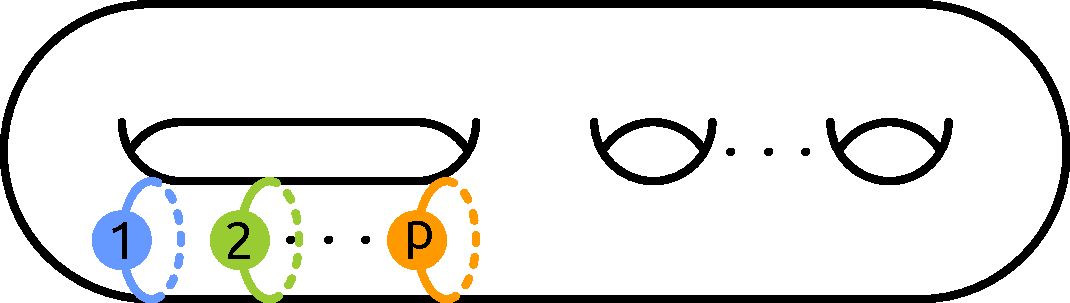
\includegraphics[width=.6\textwidth]{figures/pcolorgenus.pdf}
    \caption{A base collection of parallel nonseparating loops, as in a nest.}
    \label{fig:pcolorg}
  \end{figure}

  We first fix a collection $X$ of curves.
  If $g\geq1$, then $S_{g,p}$ has a nonseparating curve,
  and we let $X$ contain $p$ parallel nonseparating loops based at the punctures
  as in Figure \ref{fig:pcolorg}.


  If $g=0$ we take as $X=\{x_i\}_{i=1}^p$ to be as in Figure \ref{fig:pcolors}
  with $p-4$ parallel loops based at $p_2,\ldots,p_{p-2}$
  and 4 additional curves $x_1,x_2,x_{p-1},x_p$
  so that $x_1$, $x_2$ and $x_3$ pairwise intersect twice
  and are disjoint from all other curves of $X$,
  and similarly $x_p,x_{p-1},x_{p-2}$ pairwise intersect twice
  and are disjoint from all other curves of $X$.
  We will argue that each loop of $X$ must be colored differently.
  Observe that there is an arc
  $\alpha_{12}$
  from $p_1$ to $p_2$
  that is disjoint from all loops of $X$ except $x_1$ and $x_2$.
  Similarly
  there is  $\alpha_{p-1,p}$
  disjoint from all loops of $X$ except $x_p$ and $x_{p-1}$.
  So the collection $\alpha_{12},x_3,\ldots,x_{p-2},\alpha_{p-1,p}$
  require all $p$-colors to paint,
  and it must be that $f(x_1)\cup f(x_2) = f(\alpha_{12})$
  and $f(x_{p-1})\cup f(x_p) = f(\alpha_{p,p-1})$.
  So $X$ requires $p$-colors to paint.

  \begin{figure}
    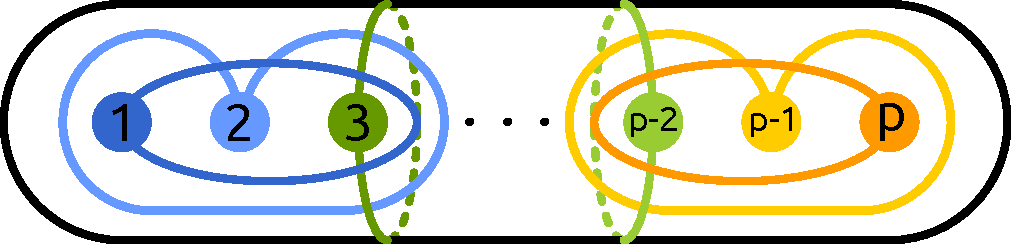
\includegraphics[width=.6\textwidth]{figures/pcolorspher.pdf}
    \caption{A base collection of mostly parallel loops in the punctured sphere.}
    \label{fig:pcolors}
  \end{figure}


  We may then assume, possibly after relabeling the colors,
  that $f$ colors the arcs of $X$ by their punctures.
  Applying Lemma \ref{putmancolor},
  we will show that the coloring on $X$ forces
  the coloring on all of $\mathcal A S_{g,p}$.
  Our technique will be to contruct paths with the group action
  of $\mcg S_{g,p}$ on $\mathcal A S_{g,p}$
  and show that $f$ is determined along these paths.
  Let $\alpha_{i,i+1}$ be an arc that is disjoint from
  all loops of $X$ except $x_i$ and $x_{i+1}$
  and contained in the annulus they bound if they are disjoint.
  Take as a generating set of $\mcg S_{g,p}$
  the Dehn half-twists along the arcs $\alpha_{i,i+1}$
  and the usual Humphrey's generators
  of Dehn twists about nonseparating curves
  that are disjoint from $X$, except for one curve $z$
  that intersects each loop of $X$ exactly once.

  We now claim that for $h \in H$ the
  coloring $f$ is determined on the loops $h\cdot X$
  by the coloring on $X$.
  We must consider several cases
  depending on whether $h$ is a twist or half-twist,
  and how $\alpha_{i,i+1}$ intersects $X$.
  These cases are considered in Figures \ref{fig:pcolor1}-\ref{fig:pcolor4}.
    \begin{figure}[h!]
      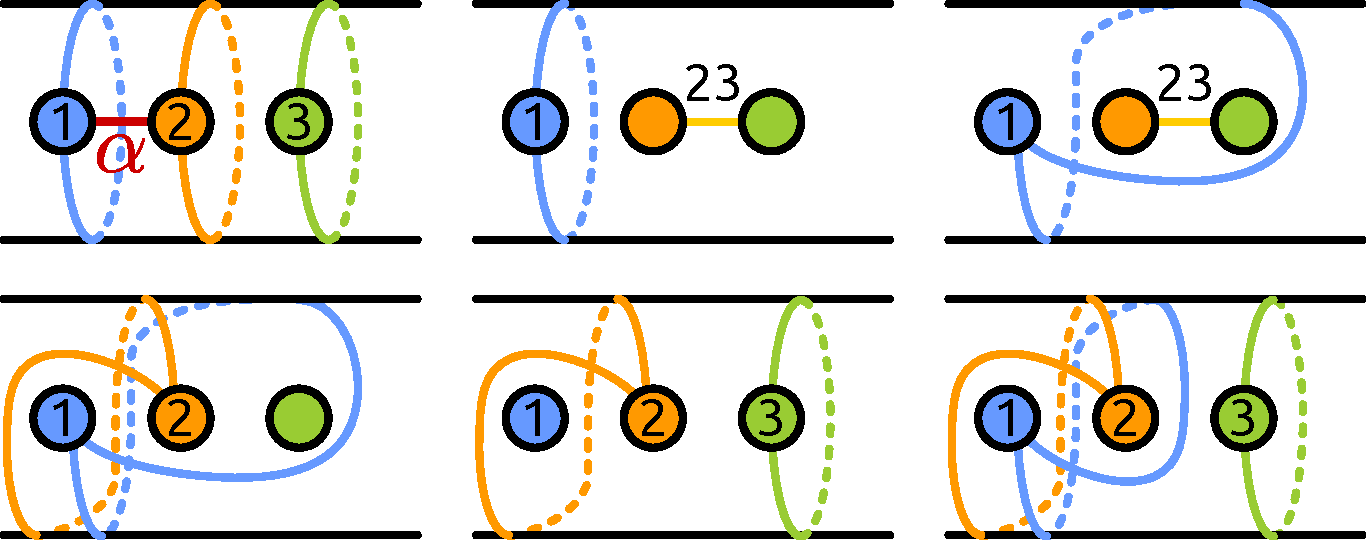
\includegraphics[width=.8\textwidth]{figures/pcolorsequence1.pdf}
      \caption{Case 1: The half-twist $h$ is about an arc $\alpha$
      in an annulus between $x_i$ and $x_{i+1}$ and disjoint from the other loops of $X$,
      as in the top left.
      The lower right shows $h(x_1)$, $h(x_2)$, and $h(x_3)=x_3$.
      Then if $f(x_i)=p_i$ the sequence of curve replacements shows
      that $f(h(x_i))=p_i$.
      }
      \label{fig:pcolor1}
    \end{figure}
    \begin{figure}[h!]
      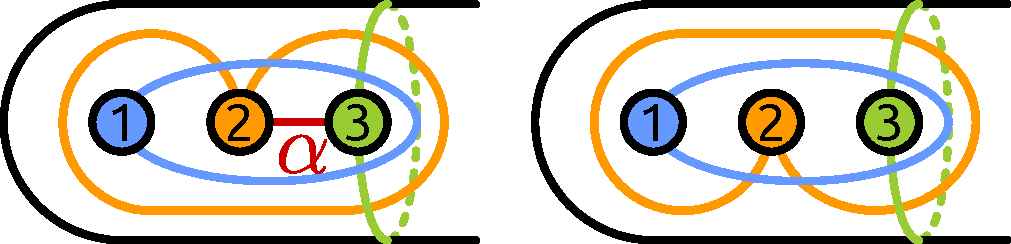
\includegraphics[width=.6\textwidth]{figures/pcolorsequence2.pdf}
      \caption{Case 2: The half-twist $h$ is about an arc $\alpha$
      $x_i$ and $x_{i+1}$ and disjoint from the other loops of $X$,
      where $x_i$ and $x_{i+1}$ intersect twice.
      We may assume the configuration on the left and note that
      $h(x_2)=x_3$, so that $f(h(x_3))$ must be $p_2$.}
      \label{fig:pcolor2}
    \end{figure}


    \begin{figure}[h!]
      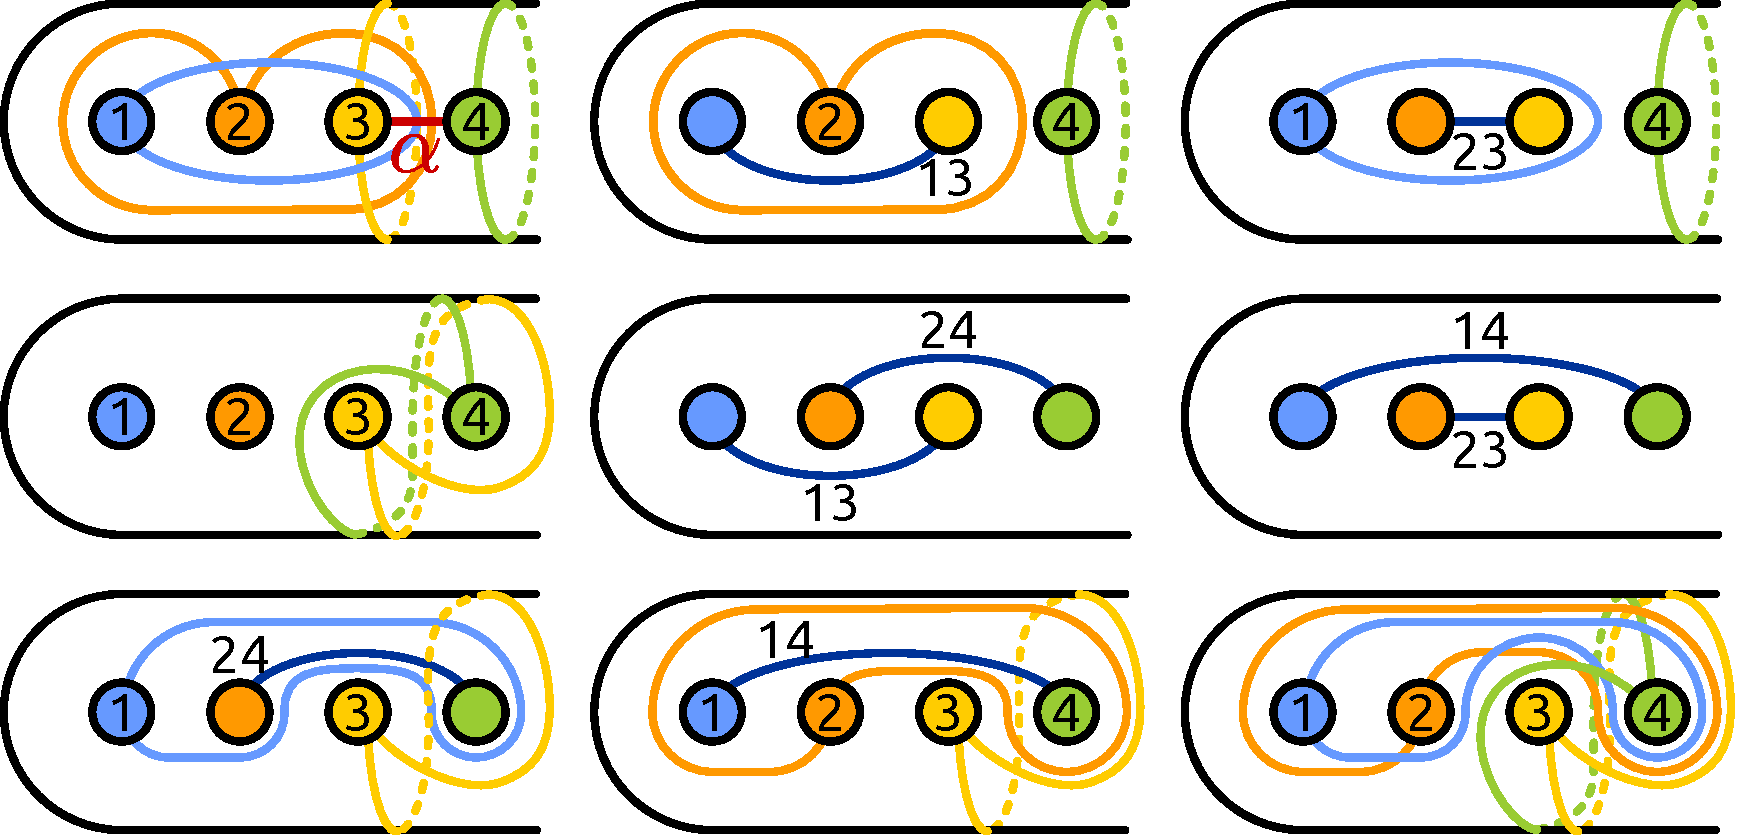
\includegraphics[width=\textwidth]{figures/pcolorsequence3.pdf}
      \caption{Case 3: The half-twist $h$ is about arc $\alpha$
      between disjoint curves $x_i$ and $x_{i+1}$,
      and $\alpha$ intersects other curves of $X$.
      We may assume the configuration on the top left.
      Then the image of $h$ is shown in the bottom right.
      Note that by Case 1, $f(h(x_3))=p_3$ and $f(h(x_4))=p_4$
      so that we need only determine $f(h(x_1))$ and $f(h(x_2))$.
      }
      \label{fig:pcolor3}
    \end{figure}
    \begin{figure}[h!]
      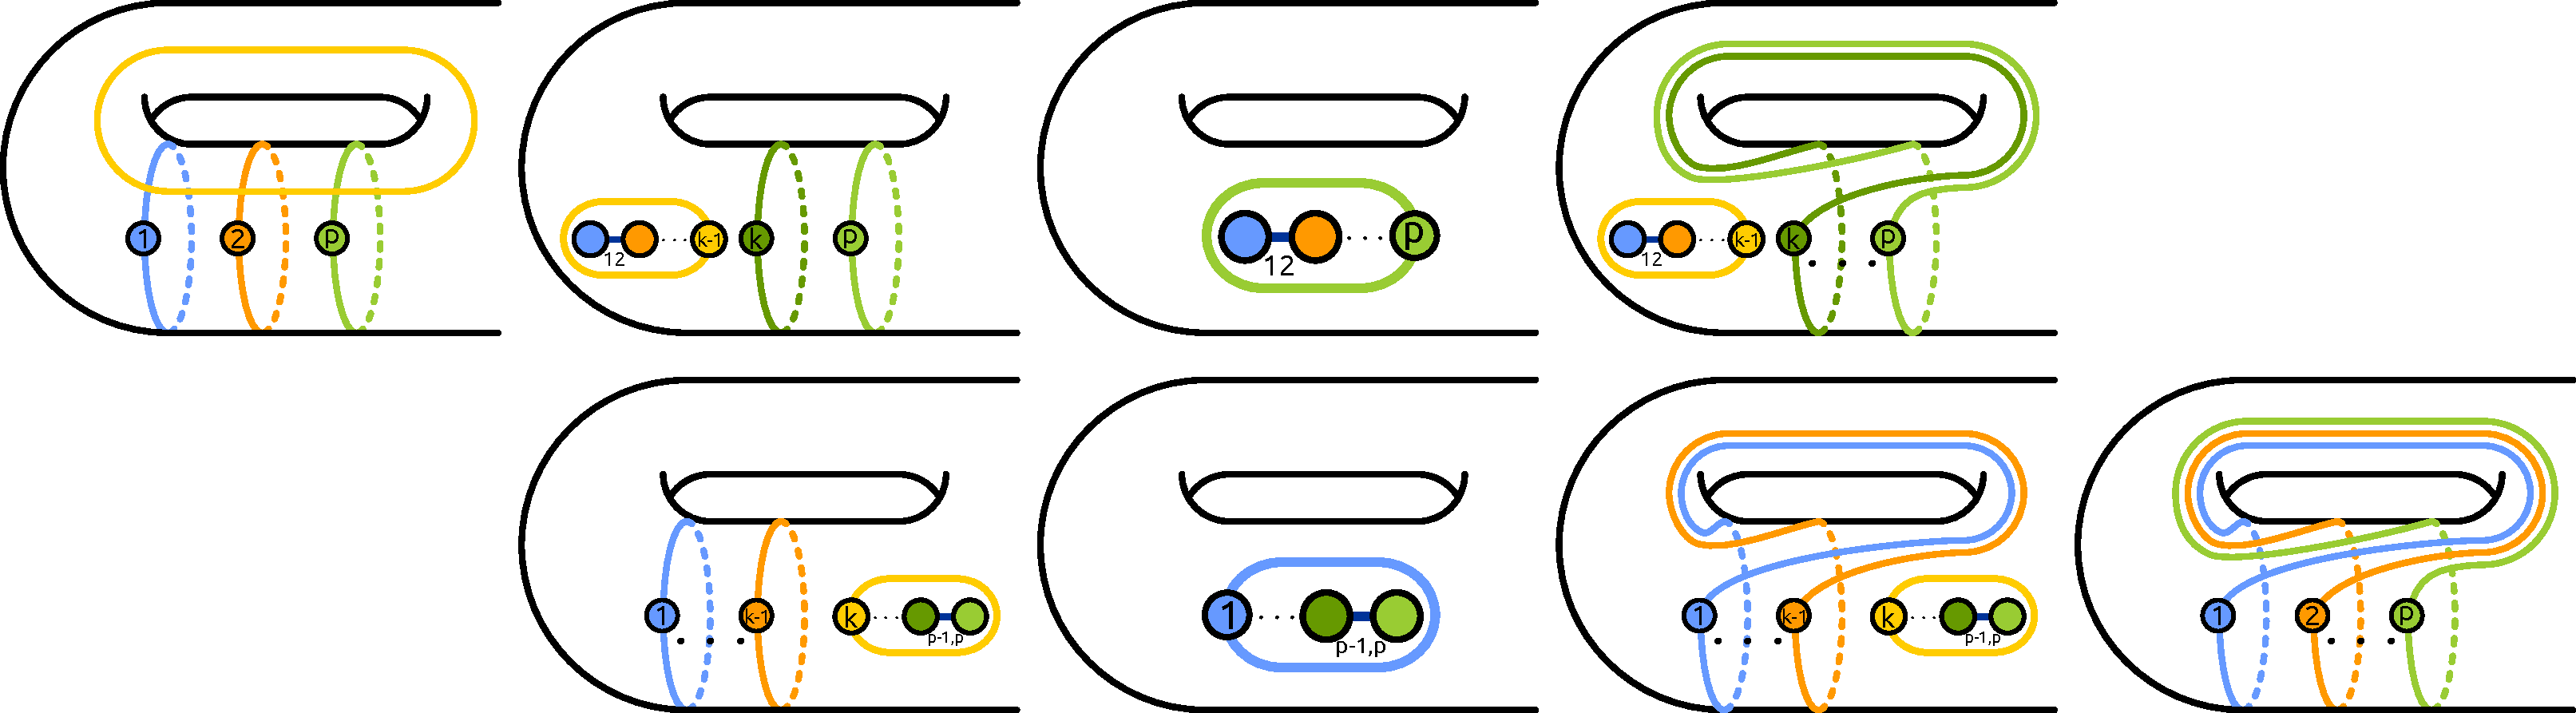
\includegraphics[width=1\textwidth]{figures/pcolorsequence4.pdf}
      \caption{Case 4: The Dehn twist $h=T_z$ about a nonseparating curve
      that links with the loops of $X$.
      We may assume the configuration of $X$ and $z$ as in the top left.
      The image $T_z(X)$ is shown in the bottom right.
      In the top row: Replace $x_1$ and $x_2$ with $\alpha_{1,2}$
      so that $f(\alpha_{12})=\{p_1,p_2\}$.
      Then iteratively replace $x_k$ with the loop $y_k$ separating
      $\alpha_{1,2},y_3, \ldots, y_{k-1}$ from the other punctures,
      so that $f(y_k)=p_k$ for $k=3,\ldots,p$.
      Then replace $y_k$ with $h(x_k)$ so that $f(T_z(x_k))=p_k$
      for $k=p, \ldots, 3$.
      A similar process reversing the order of the punctures
      as in the bottom row shows $f(T_z(x_k))=p_k$ for $k=1,\ldots,p-2$.
      }
      \label{fig:pcolor4}
    \end{figure}

  Observe that if $g \in \mcg S_{g,p}$
  we can write $g= h_n \cdots h_1$ with $h_i \in H$.
  And if the loops of $h_k \cdots h_1 \cdot X$ are painted by their punctures,
  then so are the loops of $h_{k+1} \cdots h_1 \cdot X$ by the above argument.

  Observe in the case of $g=0$ every curve is in $\mcg S_{g,p} \cdot X$.
  If $g \geq 1$ then $\mcg S_{g,p} \cdot X$ includes all nonseparating loops,
  and any separating loop $x$ is disjoint from $p-1$ mutually disjoint loops $x_1,\ldots, x_{p-1}$
  so that
  the color $f(x)$ is determined by
  the colors
  $f(x_i)$
  and so $f(x)$ must be colored by its puncture.
\end{proof}


\begin{lemma}
  Curve complex automorphisms induce
  arc complex automorphisms.

   There is a natural $\mcg^\pm S_{g,p}$ equivariant map
   $$\aaut \mathcal C S_{g,p} \to \aaut \mathcal A S_{g,p}.$$
  \label{lemma:annulus}
\end{lemma}

\begin{proof}
  By Lemma \ref{lemma:curvetype}
  automorphisms of $\mathcal S_{g,p}$
  preserve the class of two curves.
  Observe that curves $c,c'$ of $S_{g,p}$
  bound a punctured annulus if and only if there
  is a maximal simplex $\Delta \subset \mathcal C S_{g,p}$
  containing $c,c'$
  so that in the region adjacency graph $\mathcal G_\Delta$,
  the edges $e_c$ and $e_{c'}$ are incident
  at a degree 2 vertex $v_a$.
  Then applying Lemma \ref{cor:adjgraph}
  $\phi(c)$ and $\phi(c')$ must cobound a punctured annulus.

  Let $\phi \in \aaut \mathcal C S_{g,p}$
  and let $a$ be an punctured annulus $\mathcal A S_{g,p}$
  with bounding curves $c,c'$.
  If $(g,p) \neq (1,2)$ then $c,c'$ uniquely specify the annulus.
  Then $\phi(c),\phi(c')$ specify cobound a punctured annulus $\phi_\ast(a)$.

  Finally $a,a'$ are disjoint arcs if and only if
  there is a maximal simplex $\Delta \subset \mathcal C S_{g,p}$
  such that the bounding curves of regular neighborhoods of
  $a$ and $a'$
  are in $\Delta$.
  Then $a$ and $a'$ are represented by distinct
  vertices $v_a$ and $v_{a'}$ of $\mathcal G_\Delta$.
  So $a$ and $a'$ are disjoint if and only if
  $\phi_\ast (a)$ and $\phi_\ast (a')$ are disjoint.

  Thus $\phi_\ast : \mathcal A S_{g,p} \to \mathcal A S_{g,p}$
  is an isomorphism.
\end{proof}





\begin{lemma}
  Curve complex automorphism permute puncture-projection fibers.

  Let $\phi \in \aaut \mathcal C S_{g,p}$ for $3g+p \geq 6$.
  Then if $x,y$ are curves of $S_{g,p}$ with
  $\rho_q(x)=\rho_q(y)$,
  then there is a puncture $q' \in P$ such that
  $\rho_{q'}(\phi(x))=\rho_{q'}(\phi(y))$.
  \label{lemma:fibers}
\end{lemma}

\begin{proof}
  Consider the structure of $\rho^{-1}_q(\rho_q(x))$.
  We have it is a subtree of $\mathcal C S_{g,p}$
  with $x,x' \in \rho^{-1}_q(\rho_q(x))$
  adjacent if and only if they bound an annulus punctured by $q$.
  Then we have a path $x=x_0, \ldots, x_n =y$
  such that $x_i,x_{i+1}$ bound an annulus punctured by $q$.
  Using \ref{lemma:annulus}
  we have $\phi(x_i),\phi(x_{i+1})$ bound an annulus
  punctured by some $q_i$.
  Then since $x_i,x_{i+1},x_{i+2}$ bound
  annuli  punctured by $q$ that
    are the regular neighborhoods of
  loops $a_i,a_{i+1} \in \mathcal A S_{g,p}$ based at $q$.
  Then
  $\phi(x_i),\phi(x_{i+1}), \phi(x_{i+2})$
  bound annuli that are the regular neighborhoods
  of loops $\phi_\ast(a_i), \phi_\ast(a_{i+1})$.
  By Lemma \ref{lemma:paint}
  $\phi_\ast(a_i)$ and $\phi_\ast(a_{i+1})$
  are based at a common point $q'$.
\end{proof}


\begin{proof}[Proof of Theorem \ref{thm:addpunc}]
  Assume that the natural map
  $$
  \begin{tikzcd}
  \mcg^{\pm}S_{g,p-1} \arrow{r}{\gamma}& \aaut \mathcal C S_{g,p-1}
  \end{tikzcd}
  $$
  is an isomorphism.
  Then by Lemma
  \ref{lemma:exact}
  the following diagram commutes
  $$
  \begin{tikzcd}
  1 \arrow[r]&
  \pi_1(S_{g,p-1},q) \arrow[r] \arrow{d}{\alpha}&
  \mcg^{\pm}(S_{g,p},q)  \arrow{r}{f_q} \arrow{d}{\beta}&
  \mcg^{\pm}S_{g,p-1} \arrow[r] \arrow{d}{\gamma}&
  1 \\
  1 \arrow[r]&
  \pi_1(S_{g,p-1},q) \arrow{r}&
  \aaut \mathcal C (S_{g,p},q)  \arrow{r}{\rho_q}&
  \aaut \mathcal C S_{g,p-1} \arrow{r}&
  1. \\
  \end{tikzcd}
  $$
  and since $\gamma f_q = \rho_q \beta$ is a surjection we have
  that $\rho_q$ is a surjection and the rows are exact.
  By the Five Lemma $\beta$ is an isomorphism.

  Let $\phi \in \aaut \mathcal C S_{g,p}$.
  We have that by Lemma
  \ref{lemma:fibers} that
  $\phi$ permutes the fibers $\{\rho^{-1}_q\}$,
  so there is $\psi \in \mcg^{\pm}S_{g,p}$
  so that $\psi \in \aaut \mathcal C S_{g,p}$
  is such that $\psi \phi$ maintains the fibers
  $\rho^{-1}_q$.
  So $\psi \phi \in \aaut \mathcal C(S_{g,p},q)$.
  But then there is $\psi' \in \mcg^{\pm}S_{g,p}$
  so that $\psi \phi = \psi'$.
  But then $\phi = \left ( \psi^{-1}\psi' \right)$
  is also induced by a mapping class we have the natural map
  $$
  \begin{tikzcd}
  \mcg^{\pm}S_{g,p} \arrow{r} & \aaut \mathcal C S_{g,p}
  \end{tikzcd}
  $$
  is an isomorphism.
\end{proof}


\section{Spheres and Punctures}
\label{sect:spherepunc}

The main theorem of this section is the following


\outpunc*

The proof is directly analogous to our proof of Theorem
\ref{thm:addpunc}.
We will use a the structure of the puncture forgetful map and induct on the number of punctures.
A base, unpunctured case is considered by the Theorem of Aramayona and Souto \cite{souto}.

\aramsouto*

We will show that automorphisms of the punctured sphere complex
respect the fibration induced by forgetting punctures,
so that adding additional punctures expands the automorphism group
of the complex of spheres according to a Birman exact sequence.

\begin{theorem}
  If the natural map
  $$
  \oout_{n,p} \to  \aaut \mathcal  S_{n,p}
  $$
  is an isomorphism, then so is
  $$
  \oout_{n,p+1} \to  \aaut \mathcal  S_{n,p+1}
  $$
  \label{thm:outpunc}
\end{theorem}

\begin{definition}
  As in Definition \ref{def:graphadj} for surfaces, if
   $\Delta \subset \mathcal S_{g,p}$ is a simplex
  the \emph{region adjacency graph}
  $\mathcal G_\Delta$
  of $\Delta$
  is the graph whose vertices are the connected components
  of the cut manifold
  $$
  M_{n,p} - \bigcup_{x \in \Delta} x
  $$
  with an edge $e_x$ for every sphere $x$ and with
  the edge $e_x$ incident to the connected components it bounds.
  We will also consider the graph simplification
  $\mathcal G^{simp}_\Delta$.
\end{definition}

\begin{lemma}
  Sphere complex automorphisms preserve edge incidence of region adjacency graphs.

  Let $\phi \in \aaut \mathcal S_{n,p}$ and let $\Delta$ be a simplex of $\mathcal S_{n,p}$ with adjacency graph $\mathcal G_\Delta$.
  Then $e_x, e_{x'}$ are incident edges of $\mathcal G_\Delta$
  if and only if $e_{\phi(x)}, e_{\phi(x')}$ are incident
  edges of $\mathcal G_\phi(\Delta)$.
  \label{lemma:outlinegraph}
\end{lemma}

\begin{proof}
  We will argue that the induced bijection  $\phi_\ast$
  between the edges of $\mathcal G_\Delta$ and the edges of $\mathcal G_{\phi(\Delta)}$ preserves incidence.

  Let $x,x' \in \Delta$ be distinct spheres of $M_{n,p}$.
  Suppose that the associated edges $e_x$ and $e_x'$
  of $\mathcal G_\Delta$.
  It suffices to show that $e_x$ and $e_{x'}$ are incident if and only if there is a third $y \in \Delta$ with $y$
  intersecting $x$ and $x'$ but no other sphere of $\Delta$.
  In that case $e_{\phi(x)}$ and $e_{\phi(x')}$ are incident if and only if there is no third $\phi(y) \in \phi(\Delta)$ with $\phi(y)$
  intersecting $\phi(x)$ and $\phi(x')$ but no other sphere of $\phi(\Delta)$.
  So $\phi$ induces an incidence-preserving edge bijection between $\mathcal G_\Delta$ and $\mathcal G_{\phi(\Delta)}$.

  Suppose that $e_x$ and $e_{x'}$ are incident.
  Then there is a region $R$ of $M_{n,p}-\bigcup_{z \neq x,x'}z$
  containing $x$ and $x'$, and since every region of
  $M_{n,p}-\bigcup_{z \in \Delta}z$ contains at least an $M_{0,3}$,
  it must be that $R$ contains an $M_{1,2}$ or $M_{0,5}$.

  If $R$ contains an $M_{1,2}$ the subcomplex of spheres in $R$ contains a copy of $\mathcal S_{1,2}$ and so must have infinite diameter. So there must be a sphere $y$ in $R$ that intersects both $x$ and $x'$. Since $y$ is in $R$, it intersects no other sphere of $\Delta$.

  If $R$ is simply connected then it must have a copy of $M_{0,5}$
  and $x$ and $x'$ are essential and separating in $R$.
  Then there are two boundary spheres $y',y''$ of $R$ with a path $\alpha$ between them that passes through both $x$ and $x'$. Let $y$ be the boundary of a regular neighborhood of $\alpha \cup y' \cup y''$ in $R$. Then $y$ intersects both $x$ and $x'$, but since $y$ is in $R$, $y$ does not intersect any other sphere of $\Delta$.

  Suppose that $e_x$ and $e_{x'}$ are not incident.
  Then there is a collection of spheres $\Delta' \subset \Delta$
  that separate $x$ from $x'$ in $M_{n,p}$.
  So any sphere intersecting $x$ and $x'$ must also intersect a sphere of $\Delta$.
\end{proof}



\begin{corollary}
  Sphere complex automorphisms preserve the adjacency graphs of maximal simplices.

  Let $3n+p\geq 6$.
  Let $\phi \in \aaut \mathcal S_{n,p}$ and let $\Delta$ be a maximal simplex. Then $\mathcal G_\Delta$ and $\mathcal G_{\phi(\Delta)}$ are isomorphic.
  \label{lemma:outadjgraph}
\end{corollary}

\begin{proof}
  Any maximum simplex $\Delta$ contains
  $3n+p-3$ spheres and cuts $M_{n,p}$ $2n+p-2$ copies of  $M_{0,3}$.
  So $\mathcal G^{simp}_\Delta$ and $\mathcal G^{simp}_{\phi(\Delta)}$
  are simple, connected graphs with the same number of vertices and the same edge incidence relations.
  So by Whitney's Theorem  \ref{thm:whitney},
  $\mathcal G^{simp}_\Delta$ and $\mathcal G^{simp}_{\phi(\Delta)}$
  are isomorphic.

  To see that self-loops are preserved,
  observe that as $\Delta$ cuts $M_{n,p}$ into copies of $M_{0,3}$,
  every vertex of $\mathcal G_\Delta$ has degree at most 3.
  Then if $e_x$ is a self-loop at vertex $v_R$ it is incident to exactly one other edge $e_{x'}$ that cannot be a self-loop or have a parallel edge since $v_R$ is degree 3.
  So $e_{\phi(x')}$ has a degree one vertex in $\mathcal G^{simp}_{\phi(\Delta)}$.
  Since $3n+p-3\geq 3$ we have $\mathcal G_{\phi(\Delta)}$
  has at least 3 edges.
  So if both vertices of $e_{\phi(x')}$
  are degree one in $\mathcal G^{simp}_{\phi(Delta)}$, then $\mathcal G_{\phi(Delta)}$
  has two vertices with a self loop at each.
  So $e_{\phi(x)}$ is a self loop.
  If $e_{\phi(x')}$ has only one degree one vertex in $\mathcal G^{simp}_{\phi(Delta)}$, then $e_{\phi(x)}$ is only incident to $e_{\phi(x')}$. So $e_{\phi(x)}$ must be a self loop in  $\mathcal G_{\phi(\Delta)}$.

  If $\phi$ preserves both the graph simplification and the self loops of $\mathcal G_\Delta$, it must be that $\phi$ also preserves the multi-edges, and so $\phi$ induces a graph isomorphism.
\end{proof}

\begin{lemma}
  Sphere complex automorphisms preserve the topological type of spheres, and the sides of the spheres.

  Let $3n+p\geq 6$.
  Let $\phi \in \aaut \mathcal S_{n,p}$.
  Let $x$ be a sphere of $M_{n,p}$.
  Then $x$ and $\phi(x)$ have the same topological type.
  Further if $x$ is separating and $y,y'$ are spheres in the same connected component of $M_{n,p}-x$, then $\phi(x)$ is separating and $\phi(y),\phi(y')$ are
  in the same connected component of $M_{n,p}-\phi(x)$.
  \label{lemma:outspheretype}
\end{lemma}

\begin{proof}
    By Lemma \ref{lemma:outadjgraph}
    it suffices to characterise the topological type and sides of a sphere in terms of the region adjacency graph of a maximal simplex.
    \begin{enumerate}[$\cdot$]
    \item Nonseparating spheres:
    Observe that $x$ is a nonseparating sphere if and only if there is a maximal simplex $\Delta$ in that the corresponding edge $e_x$ is a self-loop in the region adjacency graph $\mathcal G_\Delta$.
    \item Separating spheres:
    Observe that if $x$ separates $M_{n,p}$
    $$
    M_{n,p} = M_{n',p'} \sqcup_x M_{n-n',p-p'+2}
    $$
    if and only if the corresponding edge $e_x$ of the region
    adjacency graph $\mathcal G_\Delta$ is a cut edge.
    More specifically, if
    $$
    \Delta=\Delta_+ \cup \{x\} \cup \Delta_-
    $$
     with $\Delta_+$ and $\Delta_-$ the spheres on each side of $x$,
     then $e_x$ separates $\mathcal G_\Delta$
     $$
     \mathcal G_\Delta - e_x = \mathcal G_{\Delta_+} \sqcup \mathcal G_{\Delta_-}
     $$
     into the components $\mathcal G_{\Delta_+}$
     with $3n'+p'-3$ edges and rank $n'$,
     and $\mathcal G_{\Delta_-}$ with
     with $3(n-n')+p-p'-1$ edges and rank $n-n'$.
  \end{enumerate}
\end{proof}

\begin{remark}
  Consider the inclusion that ignores the puncture $q$
  $$i_q: M_{n,p} \hookrightarrow M_{n,p-1}.$$
  Then for the homotopy class $[x]$ of a sphere
  in $M_{n,p}$ we have the class $[i_q(x)]$ in $M_{n,p-1}$
  by forgetting the puncture $q$.
  Separating spheres of $M_{n,p}$ bounding a copy of $S^3$ containing only $q$ and one other puncture
  will become non-essential in this inclusion,
  but other homotopy classes of spheres have well defined
  essential representatives up to homotopy forgetting $q$.

  Let $\mathcal S_{n,p}^{(q)} \subset \mathcal S_{n,p}$
  be the subcomplex for which the puncture forgetful map
  $\rho_q: [x] \mapsto [i_q(x)]$ is well defined.
  So we have a surjective projection map
  $$
  \rho_q: \mathcal S_{n,p}^{(q)} \to \mathcal S_{n,p-1}.
  $$

As in the case for surfaces, the fibers of this map are Bass-Serre trees.
% Let $\Delta$ be a simplex in $\mathcal S_{n,p-1}$.
% Let $\Delta'$ be a simplex of $\mathcal S_{n,p}$ such that $\rho_q(\Delta')=\Delta$.
Let $x$ be a sphere of $\mathcal S_{n,p-1}$.
Homotope $x$ in $M_{n,p-1}$ so that it is pointed at $q$.
Then the two boundary  spheres of a regular neighborhood of $x$ in $M_{n,p-1}$ gives a well edge of $\rho^{-1}_q(x) \subset \mathcal S_{n,p}$.
Let $\Gamma$ be the corresponding
be the graph of groups given by the splitting of $F_n=\pi_1(M_{n,p-1},q)$.
So the vertices of $\Gamma$ are the components of
$M_{n,p-1}-x$ with vertex groups given by the $\pi_1$ of the component,
and an edge with trivial edge group between two components if $x$ is separating, or a self-loop if $x$ is nonseparating.
Then there is a an isomorphism between
$\rho_q^{-1}(x)$ and the Bass-Serre tree $\tilde \Gamma$
given by associating every edge $xx'$ of $\rho_q^{-1}(x)$
with the edge of $\tilde \Gamma$ given by $uv$
if
$$
\mbox{stab}_{\pi_1(M_{n,p-1},q)}(u)
\ast
\mbox{stab}_{\pi_1(M_{n,p-1},q)}(v)
$$
is the splitting specified
by the pointed sphere at $q$ whose regular neighborhood in $M_{n,p}$ has boundary spheres
$x$ and $x'$.
\end{remark}

% \begin{lemma}
%   The fiber of the puncture forgetful map is isomorphic to the Basse Serre tree of the splitting
%   \label{lemma:outfibershape}
% \end{lemma}

\begin{definition}
  Let $\aaut(\mathcal S_{n,p},q) < \aaut \mathcal S_{n,p}$
  be the subgroup preserving the fibration of
  the forgetful map $\rho_p$.
  That is $\phi \in \aaut(\mathcal S_{n,p},q)$
  if
  $$
  \phi \left( \rho_p^{-1}\rho_p(x) \right)
  =
  \rho_p^{-1}\rho_p( \phi(x))
  $$
  for all spheres $x$.
\end{definition}

\begin{lemma}
  This diagram commutes
  $$
  \begin{tikzcd}
  1 \arrow[r]&
  \pi_1(M_{n,p-1},q) \arrow[r] \arrow[d]&
  \oout_{n,p}^{(q)}  \arrow{r}{f_q} \arrow[d]&
  \oout_{n,p-1} \arrow[r] \arrow[d]&
  1 \\
  1 \arrow[r]&
  \pi_1(M_{n,p-1},q) \arrow{r}{\alpha}&
  \aaut (\mathcal S_{n,p}, q)  \arrow{r}{\rho^\ast_{q}}&
  \aaut \mathcal S_{n,p-1} \arrow{r}&
  1 \\
  \end{tikzcd}
  $$
  and has exact rows when $\rho_{q}$ is surjective.
  \label{lemma:exactspheres}
\end{lemma}

\begin{proof}
  The map $\alpha$ is defined by the first square, so it commutes.
  The map $\alpha$ is injective, since
  for any loop $\gamma$ based at $q$,
  there is a nonseparating sphere $x$ intersecting $\gamma$
  so that the push map $\alpha(\gamma)$ acts non-trivially on $x$ and so cannot be the identity on $\mathcal S_{n,p}^{(q)}$.

  The second square must commute,
  since if $[\psi] \in \oout_{n,p}^{(q)}$
  is a mapping class of $M_{n,p}$ and $x$ a sphere of $M_{n,p}$,
  the homotopy class of $\psi(x)$ is the same if we first
  forget that the homeomorphism $\psi$ fixes $q$, or if we first allow $\psi$ with
  $q$ fixed then homotope the sphere $\psi(x)$ forgetting $q$.

  A fiber $\rho^{-1}_q(x)$ of the forgetful map
  $\rho^\ast_q: \mathcal  S_{n,p}^{(q)} \to \mathcal  S_{n,p-1}$
  is isomorphic to the Bass-Serre tree associated to the splitting.
  Then the kernel $\ker \rho^\ast_{q}$ is a
  group acting on the tree $\mathcal T_\Delta$,
  so by the
  Fundamental Theorem of Bass–Serre Theory
  \ref{thm:bassserre},
  $\ker \rho^\ast_{q}$ is isomorphic to
  the fundamental group $\pi_1$ of the
  quotient graph of groups,
  but the corresponding graph of groups is
  exactly the Van Kampen splitting of $\pi_1$ induced by $x$.
  Thus
  $$\ker \rho^\ast_{q} = \mbox{image } \alpha \cong \pi_1(S_{g,p},q)$$
  and the second row is exact.
\end{proof}

\begin{remark}
  The edges of the fibers of the forgetful map
  are between two spheres that cobound a
  $S^2 \times I$
  punctured by $q$.
  Such spheres are specified by the boundaries of regular neighborhoods of pointed spheres of $M_{n,p}$,
  so we consider the associated complex.
\end{remark}

\begin{definition}
  Let $\mathcal{PS}_{n,p}$
  be the \emph{pointed sphere complex} defined as follows.
  Let the vertices of $\mathcal{PS}_{n,p}$
  be either
  \begin{enumerate}[(1.)]
    \item pointed spheres in $M_{n,p}$, i.e. homotopy classes of maps
    $(S^2,s_0) \to (M_{n,p},P)$ where $s_0$ is a basepoint of the 2-sphere $S^2$ or else
    \item unpointed spheres that bound a twice punctured ball
  \end{enumerate}
  A collection of pointed spheres in $M_{n,p}$ span a simplex
  of $\mathcal{PS}_{n,p}$ if they have disjoint representatives, including the basepoints.
\end{definition}

\begin{definition}
As in Definintion  \ref{def:nest}, fix an order $\sigma: P \to \{1,\ldots, p\}$
let a $\sigma$-\emph{nest} of curves parallel to a sphere $x$
as the homotopy class in $M_{n,p}$
of an embedding
$$N: S^2 \times I \hookrightarrow S_{g,p}$$
such that $N$ is a homotopic to $x$ in $S_g$ by homotopy forgetting the punctures.
The image of $S^1 \times \{{\sigma(i)}/{(p-1)}\}$ is a pointed sphere based at puncture $\sigma(i)$
that we refer to as the pointed sphere $N_i$.
\end{definition}

\begin{lemma}
  The pointed sphere complex is uniquely colorable.

  % There is $p$-coloring of the 1-skeleton of $\mathcal S_{n,p}$ given by the puncture labels. Further, it is the unique $p$-coloring of
  % $\mathcal S_{n,p}$ up to permutations of the colors.
  Let $\eta(x)$ be 1 if $x$ is a pointed sphere and 2 if $x$ is an unpointed sphere that bounds a twice punctured ball of $M_{n,p}$.
  There is a unique $k,\eta$-coloring of $\mathcal {PS}_{n,p}$ given by the puncture labels.
  Further it is the only $k,\eta$-coloring up to relabeling of the $k$ colors.
  \label{lemma:outpaint}
\end{lemma}

\begin{proof}
  The argument is by the color modified Putman Lemma \ref{putmancolor}.
  Observe that if $p \leq 2$ or $n=0$ the result is trivial, so we assume $p \geq 3$ and $n \geq 1$.
  Let $f$ be any $p,\eta$-coloring of the pointed sphere complex $\mathcal{PS}_{n,p}$.

  Choose a maximal collection of nonseparating spheres $x_{a_1},\ldots,x_{a_n}$ of $M_{n,p}$
  and let $x_{b_1}, \ldots, x_{b_p}$.
  Let $H$ be the generating set of $\oout_{n,p}$ consisting of the transpositions
    $\sigma^a_{i} = (a_i a_{i+1})$
    and $\sigma^b_{i} = (b_i b_{i+1})$,
    the inversion $\iota_1$ at $a_1$ if $n=1$ or else the inversion $\iota_2$,
    the transvection $\tau_{12}$ with $a_1 \mapsto a_1a_2$ if $n\geq 2$,
    and the conjugation $\gamma_{11}$ with $b_1 \mapsto a_1b_1a_1^{-1}$.



  Let $V$ be the nest of $p$  nonseparating spheres all parallel to $x_{a_1}$
  so that $v_i$ is based at $x_{b_i}$  and separates $x^+_{a_1}, x_{b_1}, \ldots, x_{b_{i-1}}$ from
  the other spheres of $M_{n,p}$ cut along $x_{a_1},\ldots, x_{a_p}$, as in Figure \ref{fig:ptspherenest}.

  \begin{figure}[h!]
    \centering
    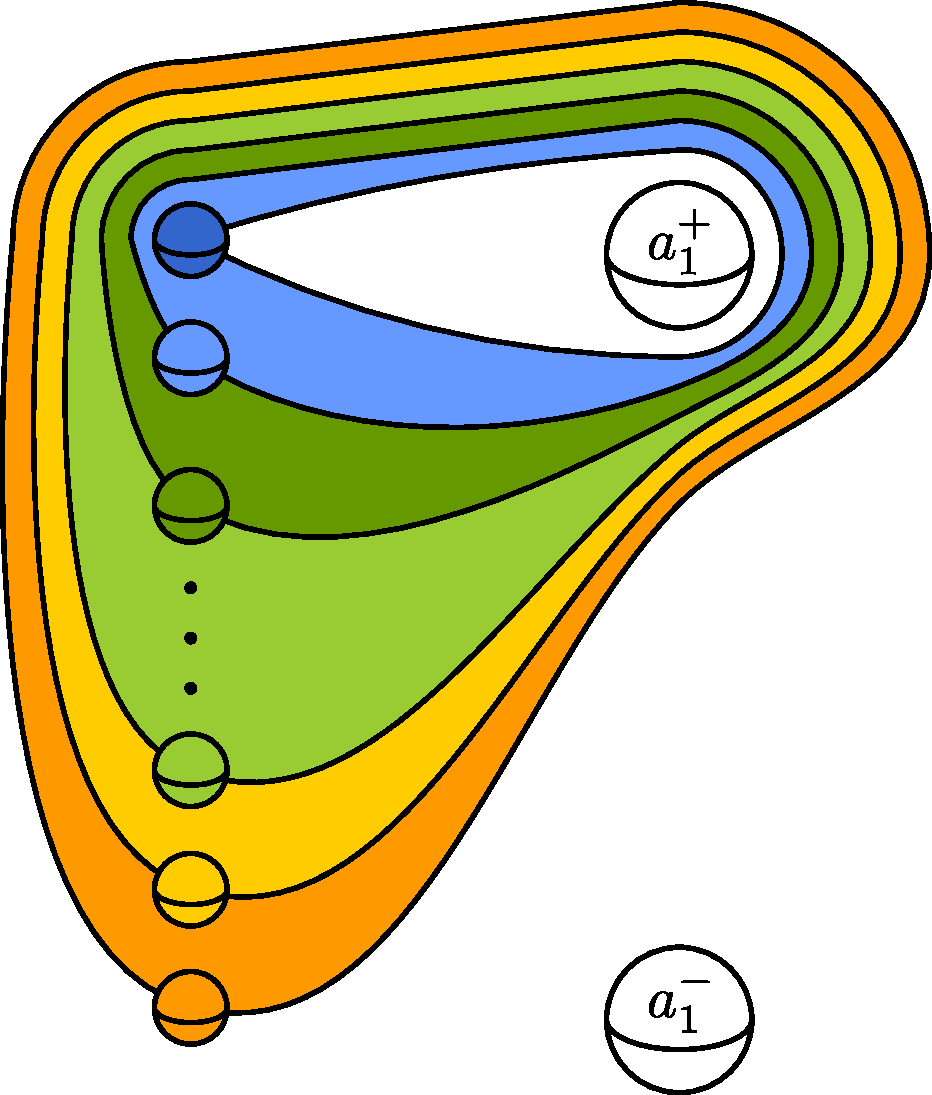
\includegraphics[width=.3\textwidth]{figures/ptspherenest.pdf}
    \caption{A nest of $p$ pointed spheres requires $p$ distinct colors.}
    \label{fig:ptspherenest}
  \end{figure}


  Since they are all disjoint they form a $p$-clique that requires they must be distinctly colored.
  We may assume, possibly after relabeling, that $f$ colors each
  pointed sphere of $V$ by the label of its puncture; so $V = \{v_i\}_{i\in P}$ and $f(v_i)=\{i\}$.

  We first show that $V$ forces a coloring on $h \cdot V$ for all $h \in H^\pm$.
  We consider the cases of the different types of generators.
  \begin{enumerate}
    \item Transvection.
    Observe that the choice of transvection is realized by the push of $x^-_{a_1}$ through
    $x^-_{a_2}$ and along a path disjoint from $v_1,\ldots,v_p$.
    So $V = \tau_{12} \cdot V$.
    \item $a$ Transposition $\sigma_i^a$. Only $\sigma_1^a$ does not fix $V$.
    Let $v_{i,j}$ be the sphere separating $x_{b_i}$ and $x_{b_j}$
    from the other spheres $x_{a_k}$ and $x_{b_\ell}$ for $\ell \neq j,k$.
    Figure \ref{fig:ptspheretransposition2} shows two sequences of forced colorings between
    $k$-colored simplices intersecting in $k-1$-colored simplices.
    The first sequence forces a coloring on $\{v_{1,2},  \sigma_1^a v_3, \ldots, \sigma_1^a v_p\}$.
    The first sequence forces a coloring on $\{\sigma_1^a v_1, \ldots \sigma_1^a v_{p-2}, v_{p-1,p}\}$.
    So $V$ forces a coloring on $\sigma_1^a \cdot V$.

    \begin{figure}[h!]
      \centering
      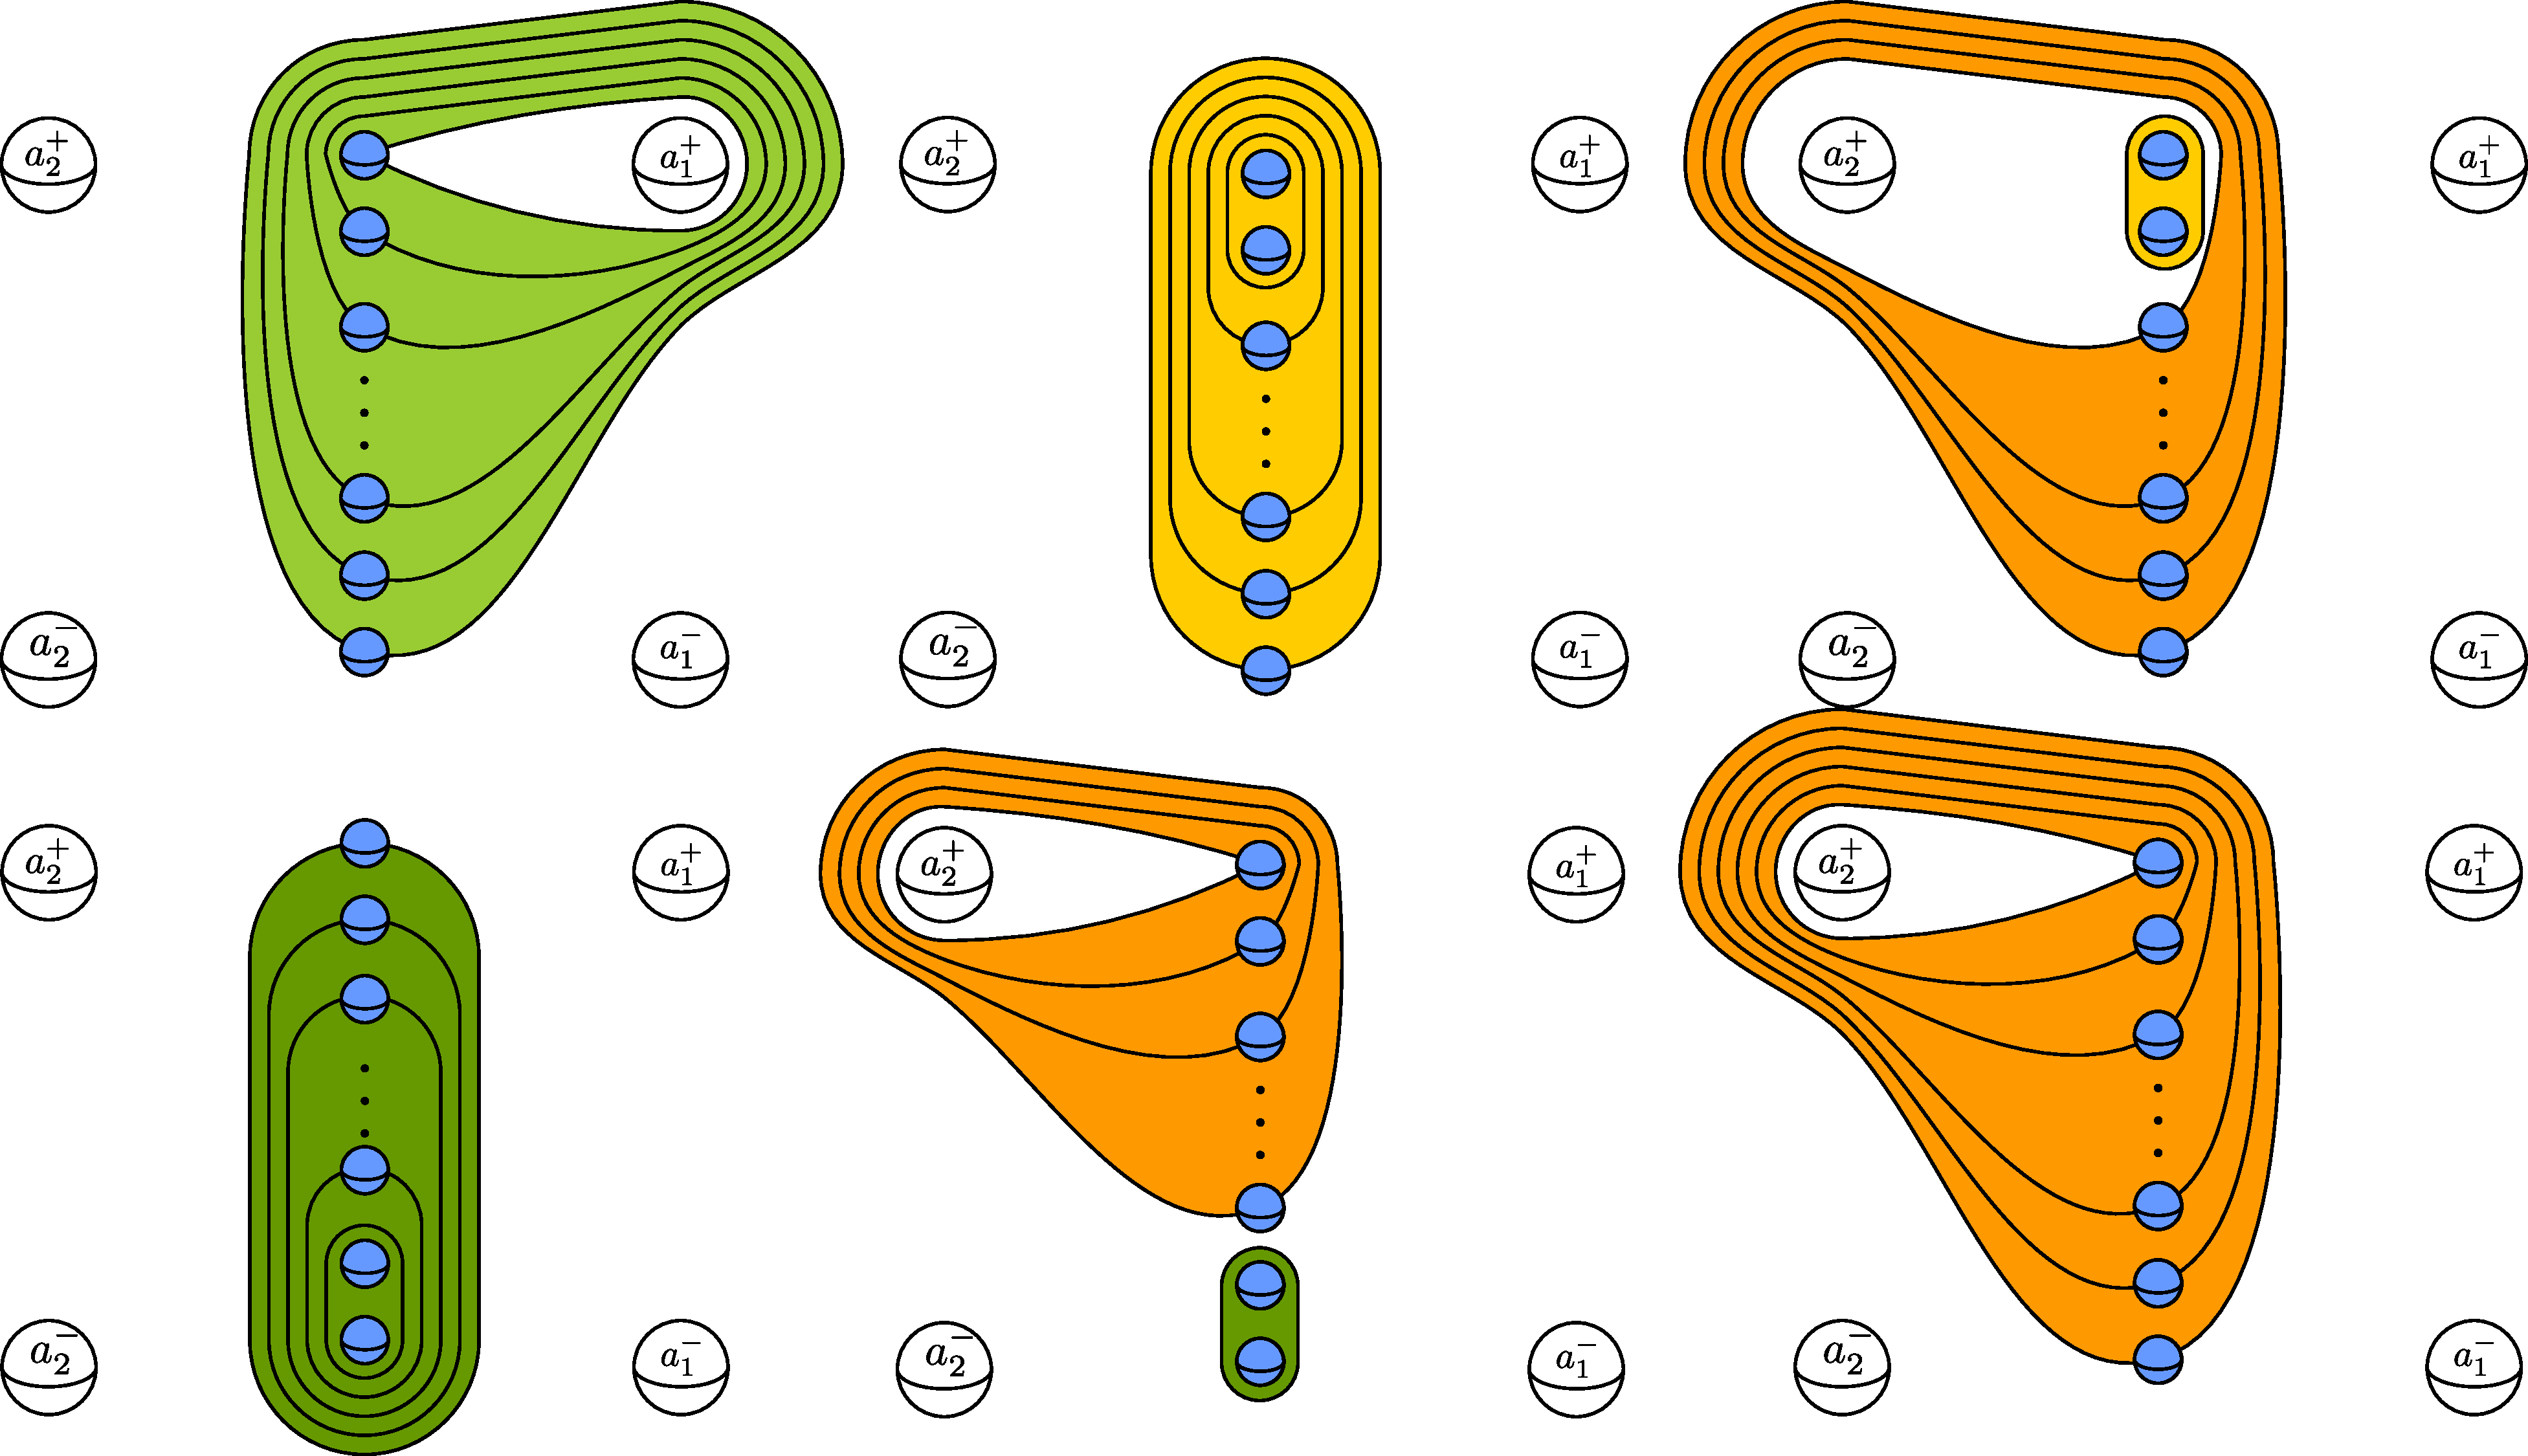
\includegraphics[width=\textwidth]{figures/ptspheretransposition2.pdf}
      \caption{A $\sigma$-nest forces a coloring on $\sigma^b_1\sigma$ nest for transposition $\sigma^a_1$.}
      \label{fig:ptspheretransposition2}
    \end{figure}

    \item $b$-transposition.
    Consider first the transposition $\sigma^b_1$.
    Figure \ref{fig:ptspheretransposition} shows a sequence of forcing colorings $\sigma^b_1$
    The argument for $\sigma^b_i$ is similar.

    \begin{figure}[h!]
      \centering
      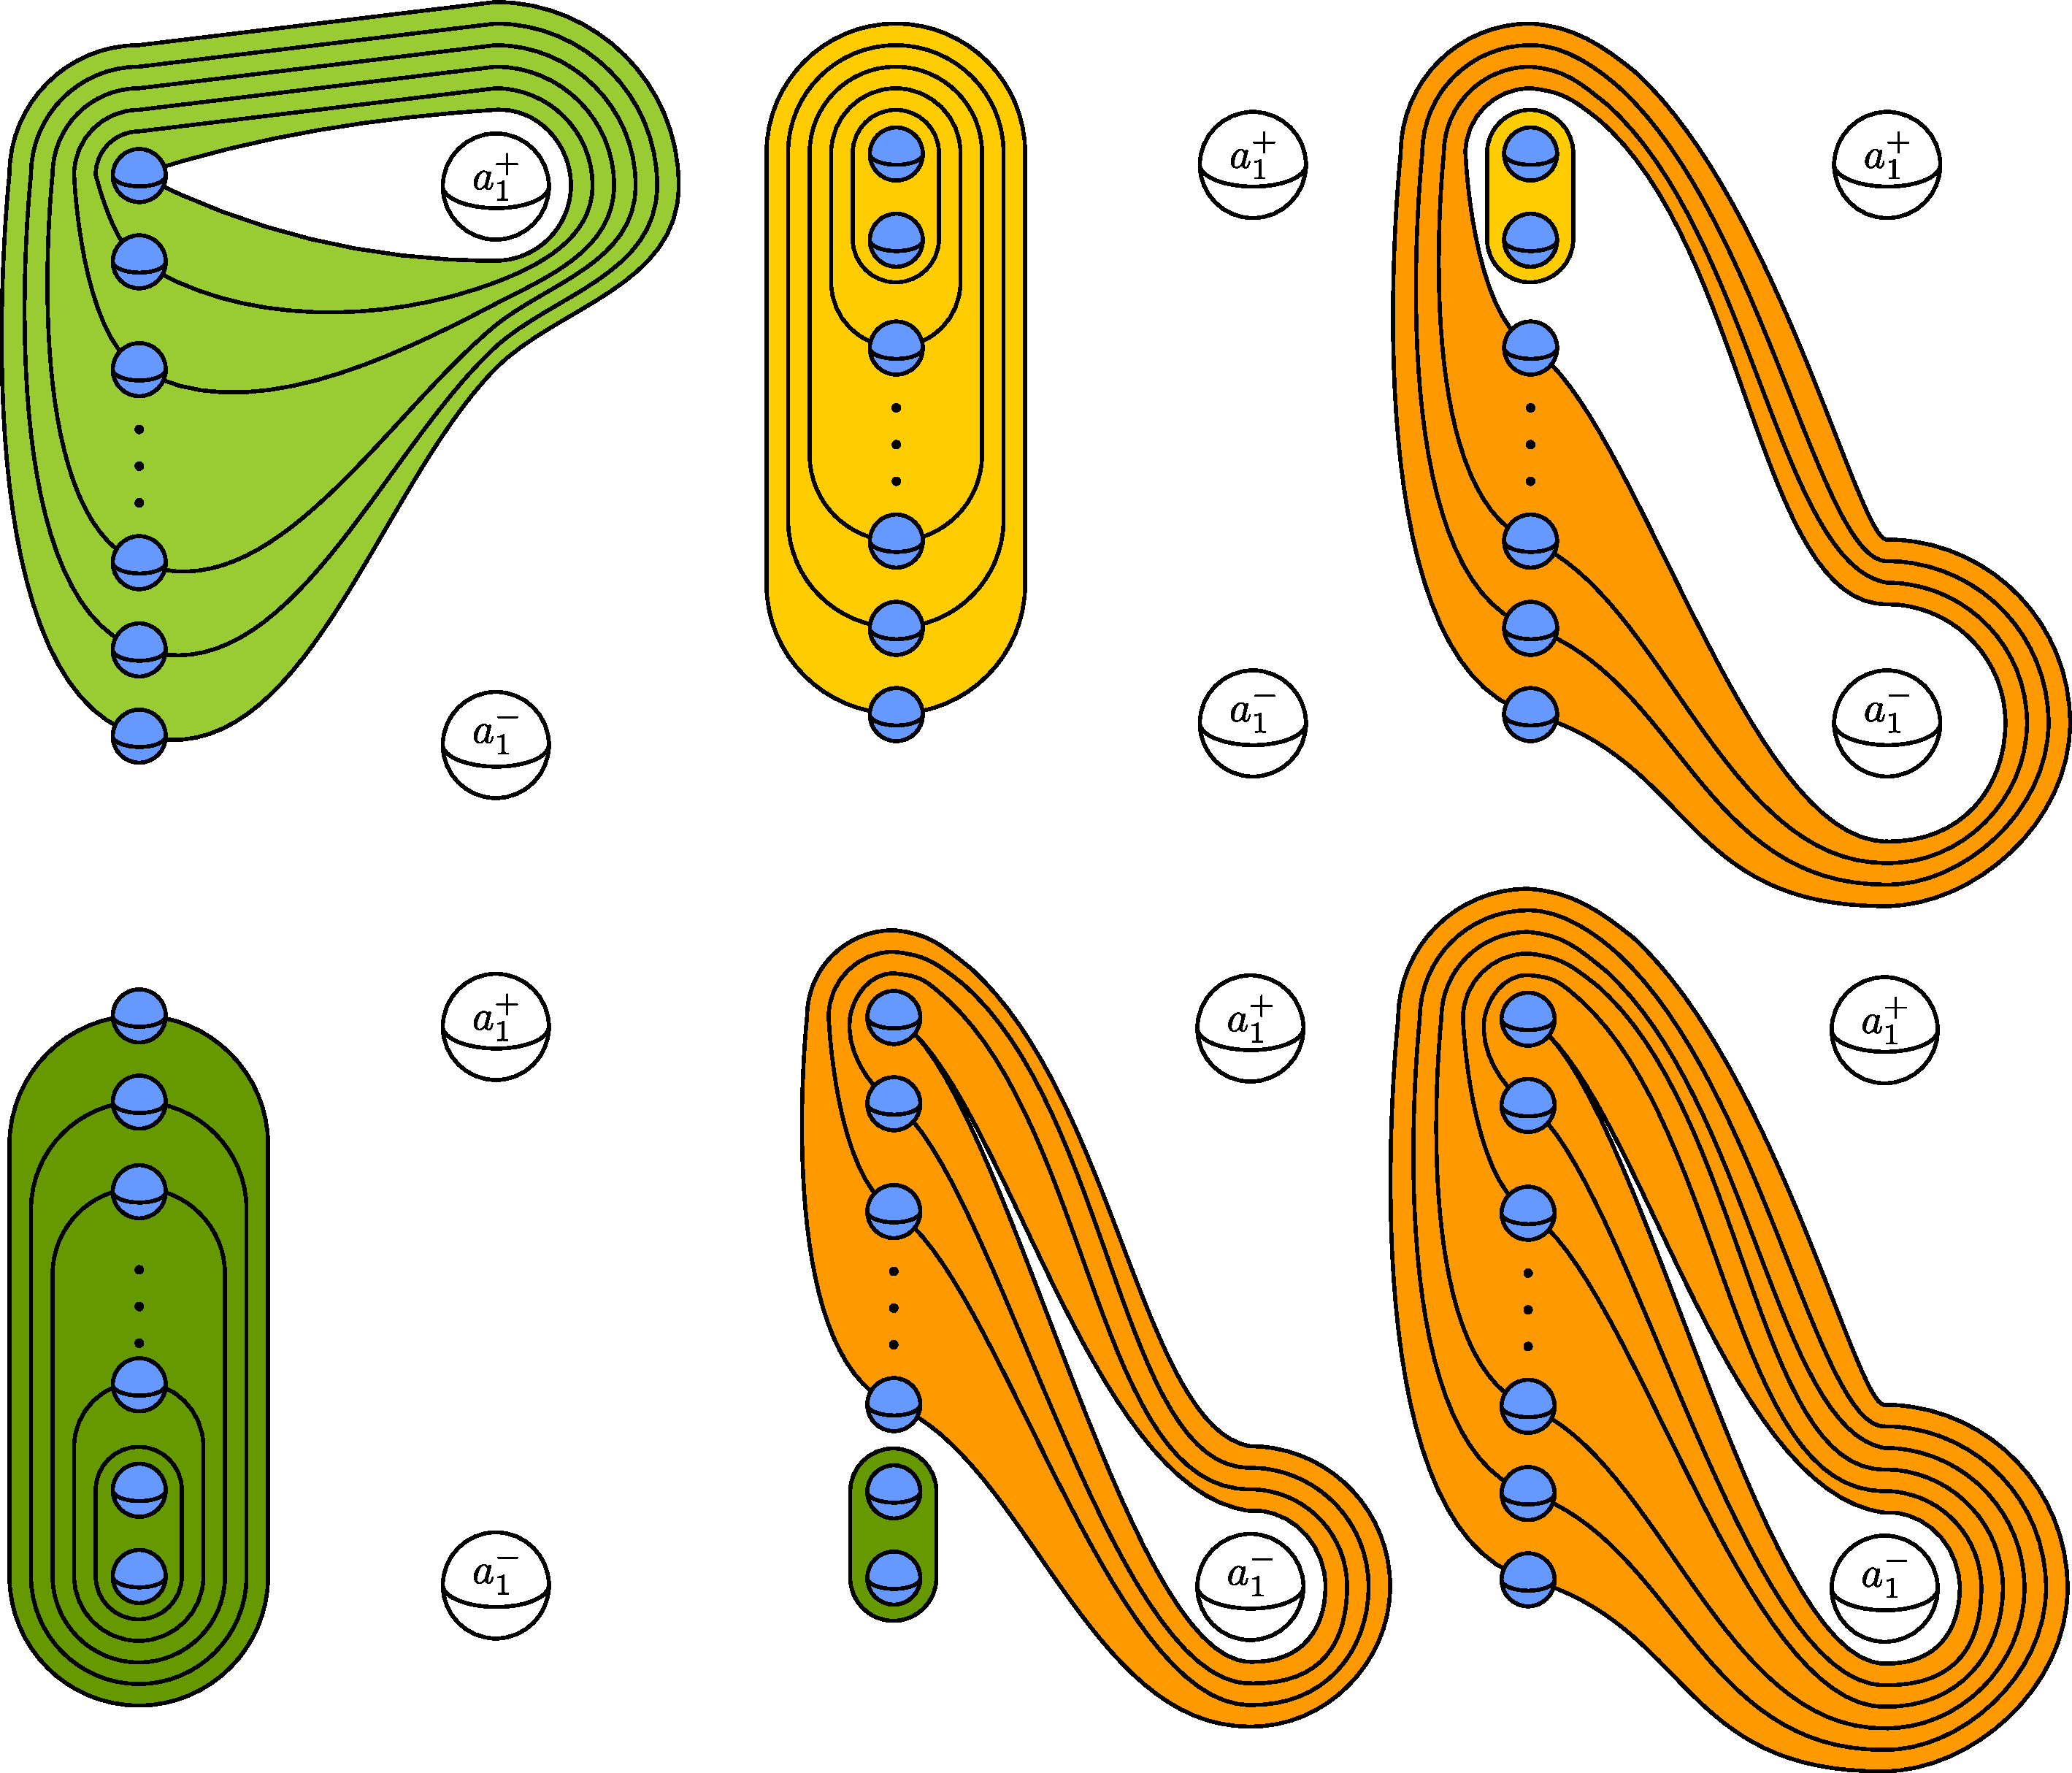
\includegraphics[width=\textwidth]{figures/ptspheretransposition.pdf}
      \caption{A $\sigma$-nest forces a coloring on $\sigma^b_1\sigma$ nest for transposition $\sigma^b_1$.}
      \label{fig:ptspheretransposition}
    \end{figure}

    \item Inversion. If $n>1$ then the inversion $\iota_2$ leaves $V$ fixed.

    If $n=1$ then Figure \ref{fig:ptsphereinversion} shows a sequence of coloring forcing.
    The first sequence forces a coloring on $\{v_{1,2},  \iota_1 v_3, \ldots, \iota_1 v_p\}$.
    The first sequence forces a coloring on $\{\iota_1 v_1, \ldots \iota_1 v_{p-2}, v_{p-1,p}\}$.
    So $V$ forces a coloring $\iota_1 \cdot V$.

    \begin{figure}[h!]
      \centering
      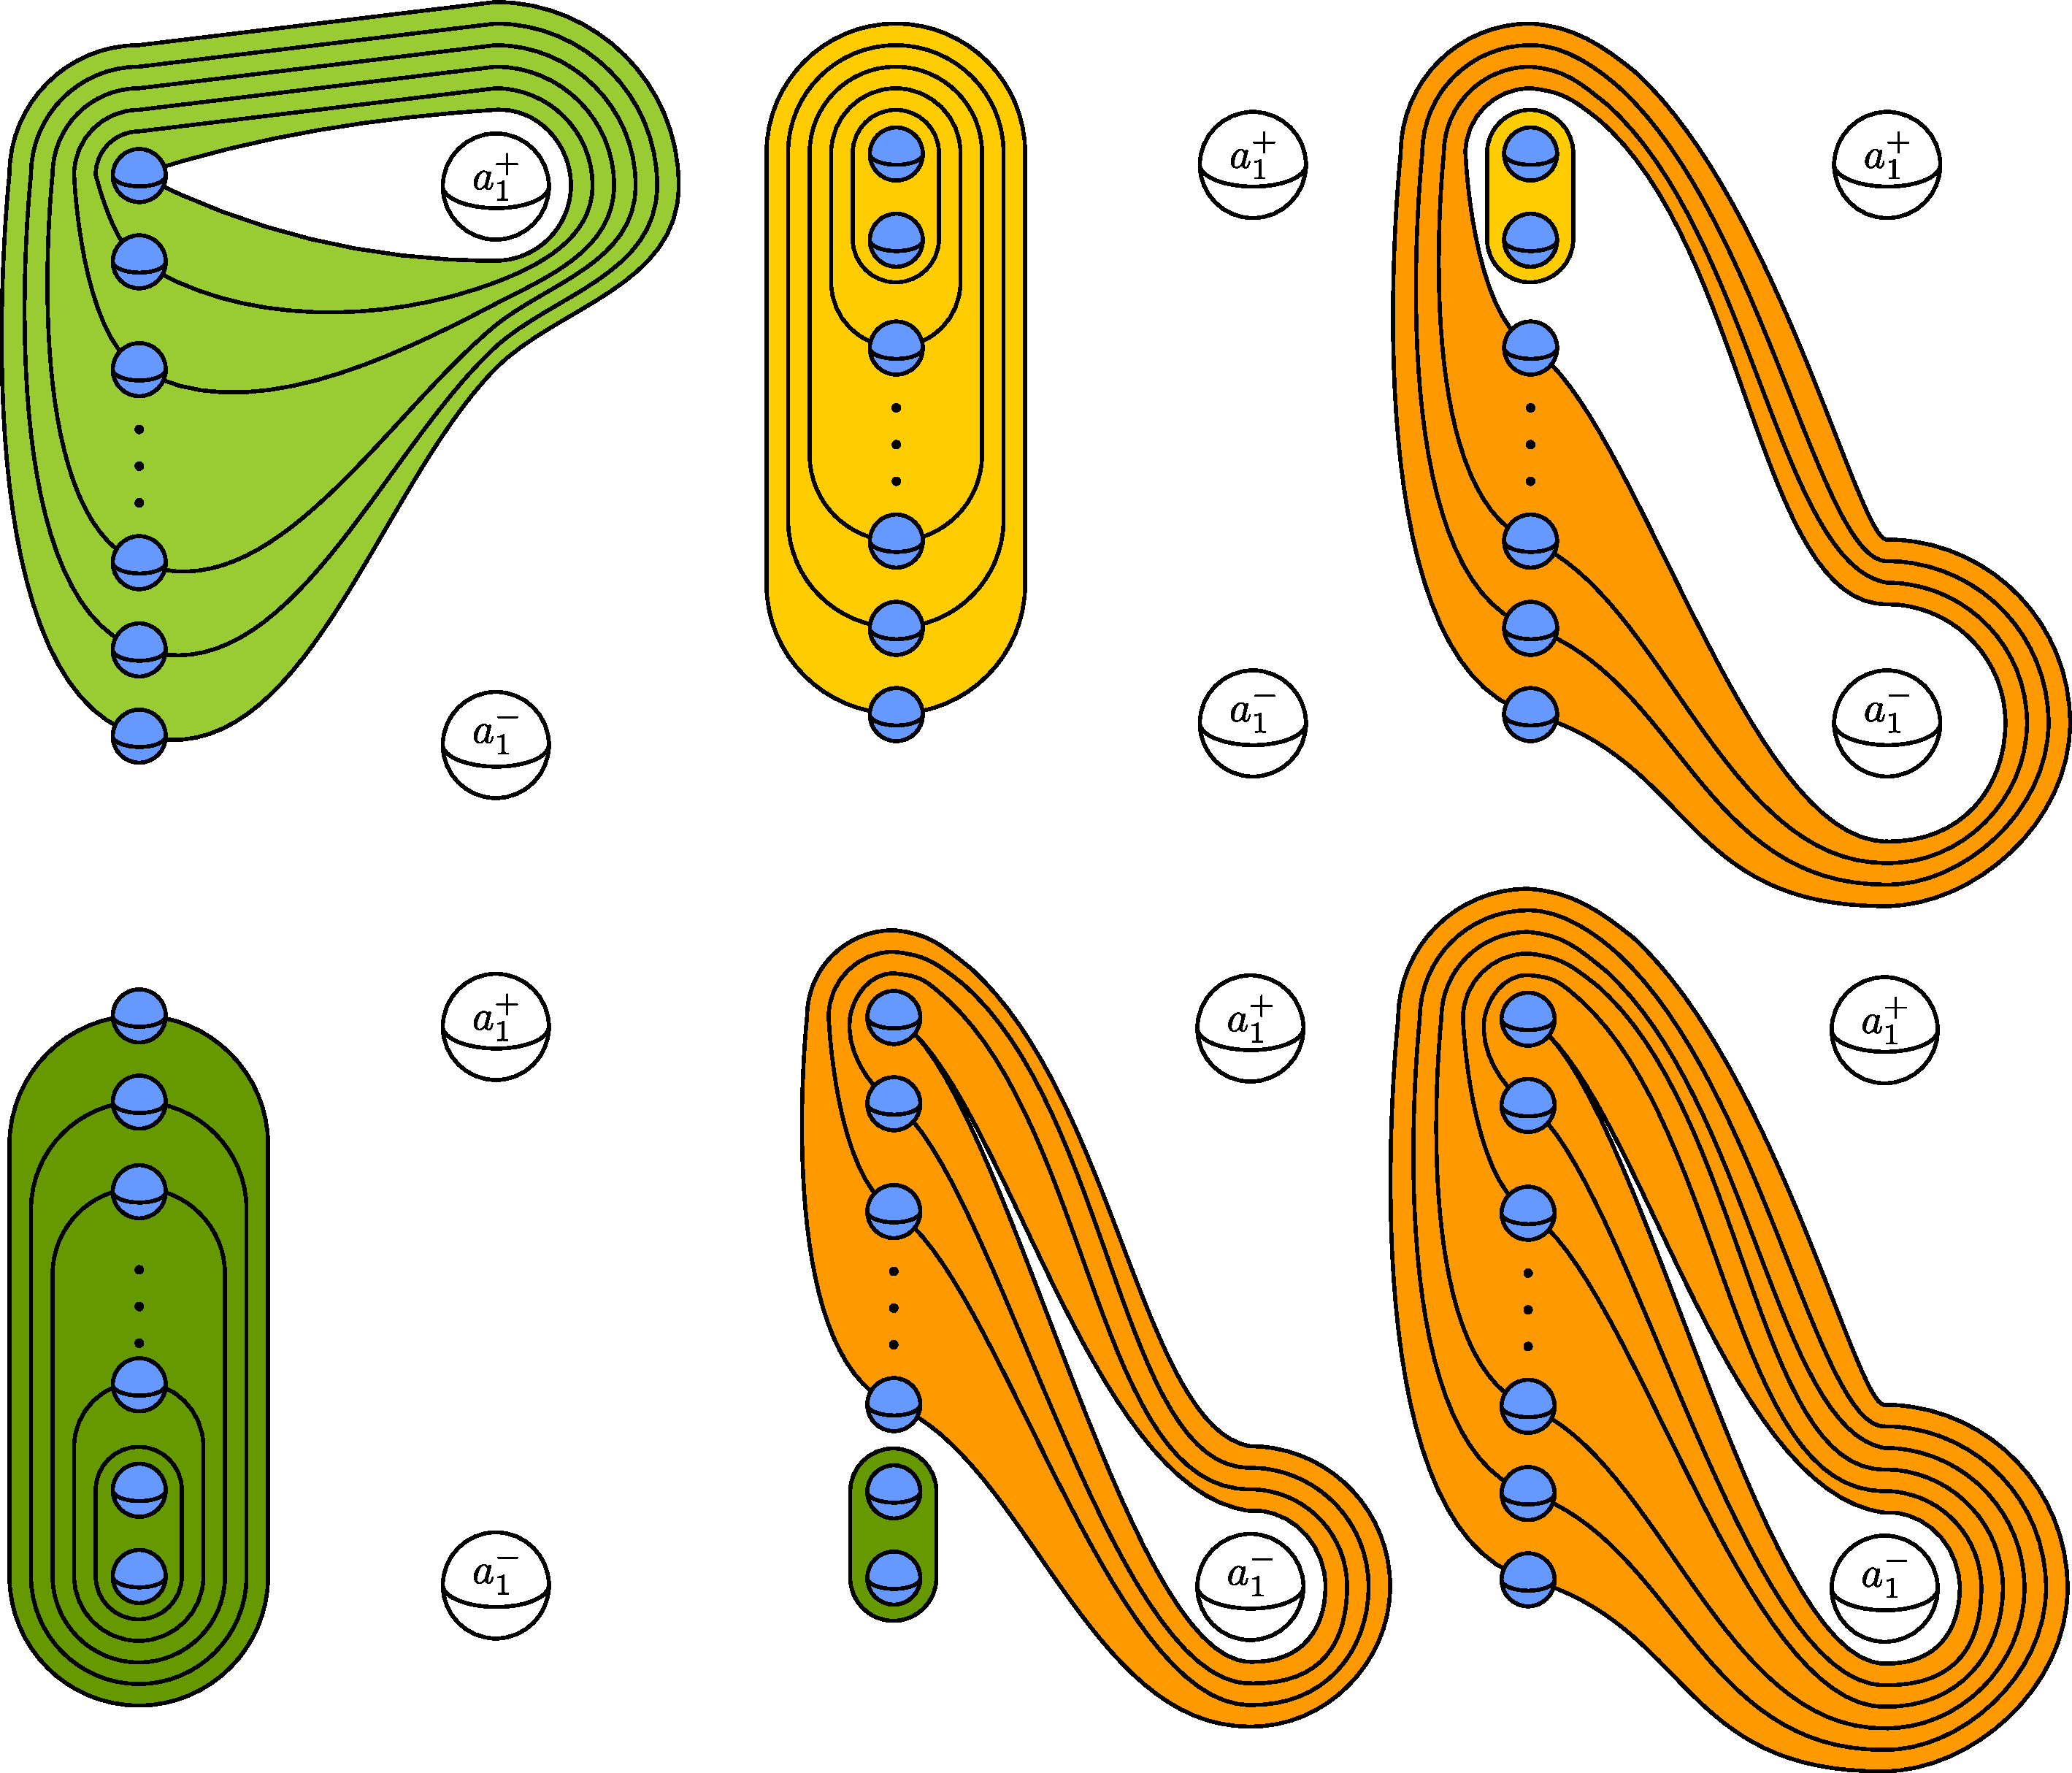
\includegraphics[width=\textwidth]{figures/ptsphereinversion.pdf}
      \caption{Two sequences together show the nest $V$ forces a coloring on $\iota_1V$.}
      \label{fig:ptsphereinversion}
    \end{figure}

    \item Conjugation. Figure \ref{fig:ptsphereconj} shows a sequences of forced colorings between
    $k$-colored simplices intersecting in $k-1$-colored simplices.
    from $V$ to $\tau_{12} \cdot V$.
    The case for $\tau^{-1}_{12}$ is similar.

    \begin{figure}[h!]
      \centering
      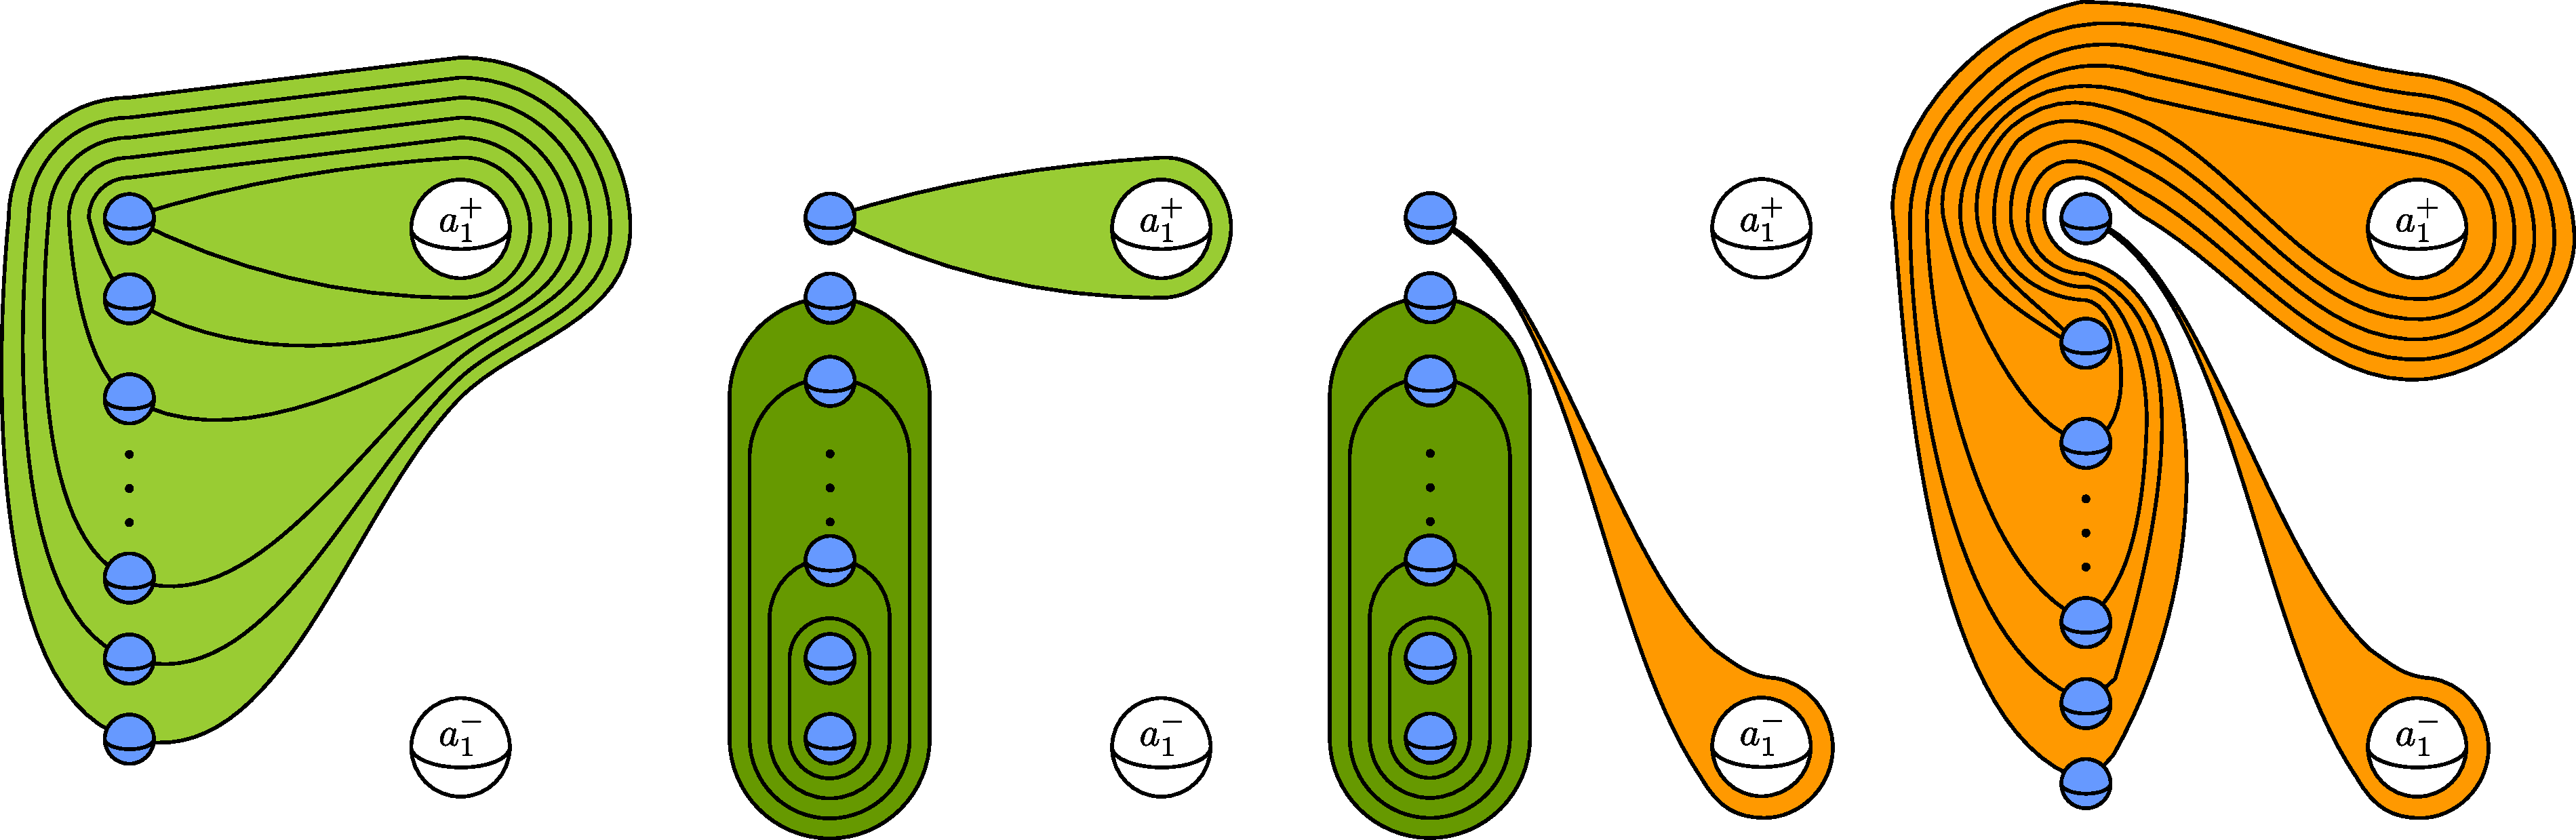
\includegraphics[width=\textwidth]{figures/ptsphereconj.pdf}
      \caption{The nest $V$ forces a coloring on $\tau_{12}V$.}
      \label{fig:ptsphereconj}
    \end{figure}
  \end{enumerate}
  From this we have that $V$ forces a coloring on its orbit $\oout_{n,p} \cdot V$.

  Finally we argue that $\oout_{n,p} \cdot V$ forces a coloring on $\mathcal S_{n,p}$.
  Let $V_k \subset \mathcal{PS}_{n,p}^{(0)}$ be the set of all
  unpointed separating spheres bounding $M_0,3$ and
  pointed separating spheres bounding $M_{0,j}$ for $j\leq k$.
  If $x \in V_3$, then we may find a collection of $k-2$ pointed nonseparating spheres that are
  disjoint from each other and from $x$.
  Then since $\oout_{n,p} \cdot V$ contains all pointed nonseparating spheres the coloring is determined on $x$.
  So $\oout_{n,p} \cdot V$ forces a coloring on $V_3$.
  Inductively we have that $V_k \cup \oout_{n,p} \cdot V$ forces a coloring on $V_{k+1} \cup \oout_{n,p} \cdot V$.
  So $V$ forces a coloring on $V_{p-1} \cup \oout_{n,p} \cdot V$.
  Then if $x$ is any pointed separating sphere,
  there are $p-1$ pointed curves or separating spheres bounding an $M_{0,3}$ that are mutually disjoint and disjoint from
   $x$.
  So $V_{p-1} \cup \oout_{n,p} \cdot V$ forces a coloring on $x$.
  Since $x$ was an arbitrary separating sphere, $V_{p-1} \cup \oout_{n,p} \cdot V$.
  The result then follow from Lemma \ref{putmancolor}.
\end{proof}

\begin{lemma}
  Sphere complex automorphisms induce automorphisms of the based sphere complex.

  There is a natural $\oout_{n,p}$-equivariant map
  $\aaut \mathcal S_{n,p} \to \aaut \mathcal{PS}_{n,p}$.
  \label{lemma:outbasedspheres}
\end{lemma}

\begin{proof}
  Let $\phi \in \aaut \mathcal S_{n,p}$ by an automorphism of the sphere complex.

  According to Lemma \ref{lemma:outspheretype} the automorphism $\phi$
  preserves the class of separating spheres bounding $M_{0,3}$.
  Suppose that $x$ is a pointed sphere of $M_{n,p}$.
  Then a regular $R$ neighborhood of $x$ is an $M_{0,3}$
  with a puncture and bounded by two spheres $x',x''$ of $M_{n,p}$.
  Observe that two spheres of $\mathcal S_{n,p}$ cobound an $M_{0,3}$
  with a puncture if and only if they are in a maximal simplex $\Delta$
  such that the corresponding vertex in the region adjacency graph $\mathcal G_\Delta$
  is degree 2.
  By Lemma \ref{lemma:outadjgraph} the adjacency graph $\mathcal G_{\phi(\Delta)}$
  is isomorphic to $\mathcal G_\Delta$,
  and $\phi(x')$ and $\phi(x'')$ bound a regular neighborhood of a punctured sphere $\hat \phi(x)$,
  and the map $x \mapsto \hat \phi(x)$ gives an isomorphism of $\mathcal {PS}_{n,p}$.
  Further $\phi \mapsto \hat \phi$ is an injection since every sphere of $M_{n,p}$
  is a boundary component for a regular neighborhood of some pointed sphere of $M_{n,p}$.
  Hence if $\hat \phi$ is the identity, so must $\phi$ be.
\end{proof}

\begin{lemma}
  Sphere complex automorphisms permute the fibers of the puncture forgetful map.
  Let $\phi \in \aaut \mathcal S_{n,p}$ and $x \in \mathcal S_{n,p}$.
  Then
  $$
  \phi \left ( \rho^{-1}_q\rho_q(x) \right )
  =\rho^{-1}_{q'}\rho_{q'}( \phi(x))
  $$
  for some $q' \in P$.
  \label{lemma:outfibers}
\end{lemma}

\begin{proof}
  Observe that an edge of $\mathcal S_{n,p}$
  in $\rho^{-1}_q\rho_q(x)$ specifies a punctured sphere of $\mathcal {PS}_{n,p}$
  colored by $q$.
  If $x,x' \in \rho^{-1}_q\rho_q(x)$ then we have a path
  $x=x_0, \ldots, x_n=y$ with $x_{i-1},x_{i}$  cobounding an $M_{0,3}$ that is the
  regular neighbodhood of punctured sphere $y_i$.
  Then by Lemma \ref{lemma:outbasedspheres} $\phi$ induces an automorphism $\hat \phi \in \mathcal{PS}_{n,p}$ such that $\phi(x_{i-1}),\phi(x_{i})$
  cobound a neighborhood of $\hat \phi(y_i)$.
  By Lemma \ref{lemma:outpaint} $\mathcal{PS}_{n,p}$ is uniquely colored by the punctures, so
  since $y_i$ are all colored by $q$ and $\hat \phi$ must permute the colors we have that
  $\hat \phi(y_i)$ are all punctured spheres based at the same point $q'$ and give the edges for the path
  $\phi(x_0), \ldots, \phi(x_n)$ in $\rho^{-1}_{q'}\rho_{q'}(x)$.
\end{proof}


\begin{proof}[Proof of Theorem \ref{thm:outpunc}]
Suppose that the natural map
$$
\begin{tikzcd}
\oout_{n,p-1} \arrow{r}{\gamma}& \aaut \mathcal S_{n,p-1}
\end{tikzcd}
$$
is an isomorphism.
Then according to Lemma
\ref{lemma:exactspheres} the following diagram commutes
$$
\begin{tikzcd}
1 \arrow[r]&
\pi_1(M_{n,p-1},q) \arrow[r] \arrow[d]&
\oout_{n,p}^{(q)}  \arrow{r}{f_q} \arrow{d}{\beta}&
\oout_{n,p-1} \arrow[r] \arrow[d]&
1 \\
1 \arrow[r]&
\pi_1(M_{n,p-1},q) \arrow{r}{\alpha}&
\aaut (\mathcal S_{n,p}, q)  \arrow{r}{\rho_{q}}&
\aaut \mathcal S_{n,p-1} \arrow{r}&
1 \\
\end{tikzcd}
$$
and has exact rows
since $\rho_q$ is a surjection as $\gamma f_q = \rho_q \beta$
is. By the Five Lemma we have $\beta$ is an isomorphism.
Let $\phi \in \aaut \mathcal S_{n,p}$.
By \ref{lemma:outfibers} $\phi$ permutes the fibers of the maps $\rho_q$,
so there is $\psi \in \oout_{n,p}$ such that
$\psi \phi$ preserves $\rho^{-1}_q \rho_q$.
But then  $\psi \phi \in \aaut \mathcal S_{n,p}^{(q)}$, and by the exact sequence
there is $\psi' \in \oout_{n,p}$ such that $\psi \phi=\psi'$.
But then $\phi = \psi^{-1} \psi'$ is also in $\oout_{n,p}$.
It follows that the natural map
$$
\begin{tikzcd}
\oout_{n,p} \arrow{r}{\gamma}& \aaut \mathcal S_{n,p}
\end{tikzcd}
$$
is an isomorphism.
\end{proof}


% !TEX root = thesis.tex
\chapter{Further Out}
\label{chap:furout}

In this chapter we advance the goal of
an $\oout F_n$ analog to
the
Brendle-Margalit Theorem \cite{meta}
by considering subcomplexes of the
sphere complex $\mathcal S_n$
that are themselves combinatorial models.
We will largely argue by extending automorphisms
from subcomplexes of $\mathcal S_n$ to automorphisms
of $\mathcal S_n$ by finding a combinatorial characterization
of any absent type of sphere.

In Section
\ref{sect:sepspheres} we consider the complex of separating spheres.
In Section
\ref{section:highgenussep}
we consider the complex of separating sphere with sufficiently complex sides.
In Section \ref{section:ffc}
we consider the complex of coconnected spheres and its relation to the free factor complex.


\section{Complex of Separating Spheres}
\label{sect:sepspheres}

Let $\mathcal {S}^{sep}_{n,p} \subset \mathcal {S}_{n,p}$ be the complex of embedded homotopy classes of separating spheres
in $M_{n,p}$. In this section we will aim to show that the complex of separating spheres is a combinatorial model for $\oout_{n,p}$.

\thmsepspheres*

We begin by computing the dimension.

\begin{lemma}
\label{sepflagdim}
$\mathcal {S}^{sep}_{n,p}$ is a flag complex of dimension $2n+p-4$.\\
\end{lemma}
\begin{proof}
$\mathcal {S}^{sep}_{n,p}$ is the induced subcomplex of $\mathcal {S}_{n,p}$,
which is known to be flag \cite{souto}.
We show by induction that any collection $\Sigma$ of disjoint spheres
in $M_{n,p}$
is a subset of a
maximal collection of $\max(2n+p-3,0)$ disjoint spheres.

Suppose for a base case that $\Sigma = \varnothing$.
Any pants decomposition of the surface $S_{n,p}=\partial H_{n} - P$ by curves surrounding
disks in the handlebody $H_n$ with punctures $P$ has
$3n-3+p$ curves with $n$ of them nonseparating.
Taking an identical copy of $\partial H_{n}-P$ and gluing along $S_{n,p}$
promotes the pants decomposition of $S_{n,p}$ into a decomposition of $M_{n,p}$ into $M_{0,3}$s.
Of these $3n-3+p$ spheres, $n$ are nonseparating and $2n+p-3$ are separating.

Assume that any collection of $k$ or fewer disjoint spheres in $M_{n,p}$ is a subset of a
maximal collection of $2n+p-3$ disjoint spheres.
Let $\Sigma$ be a collection of $k$ disjoint spheres and let $x$
be a sphere disjoint from all spheres of $\Sigma$.
Then cutting $M_{n,p}$ along $x$ yields two components
homeomorphic to
$M_{n',p'}$ and $M_{n'',p''}$ where $n'+n'' =n$ and $p'+p''=p+2$.
By inductive hypothesis, the set spheres of $\Sigma$ in each component can
extended to maximal sets $\Sigma_1$ and $\Sigma_2$ of size
$2n'+p'-3$
and
$2n''+p''-3$
respectively.
Then $\Sigma \cup \{x\}$ is contained in the maximal set
$\Sigma_1 \cup \Sigma_2 \cup \{x\}$ of size
$$
(2n'+p'-3) + (2n''+p''-3) + 1 =2n+p-3.
$$
\end{proof}


\begin{lemma}
  $\mathcal {S}^{sep}_{n,p}$ is connected
whenever it has positive dimension, except if
$(n,p)=(2,1)$.
\end{lemma}


\begin{proof}
Consider first the case where $n=0$.
There is a deformation retraction of $M_{0,s}$ away from the puncture $p_s$ to a wedge product $\bigvee_{i \in s-1}S^2_i$ of $p-1$ copies of $p^2$.
We thus have $\pi_2(M_{0,s}) \cong \Z^{s-1}$.
If $x$ is an embedded sphere of $M_{0,s}$ separating the set of punctures $\{p_{i_1}, \ldots, p_{i_k}\}$ from the other punctures, then the map
$$
\begin{tikzcd}
x \arrow[hookrightarrow]{r}
& M_{0,s}  \arrow{r}
& \bigvee_{i \in s-1}S^2_i \arrow{r}
 &S^2_{p_k}
\end{tikzcd}
$$
is degree 1 if $x$ separates $p_k$ from $p_s$ and 0 otherwise.
(See degree theory of \cite{MR1867354}.)
So there are $2^{s-1}-1$ homotopy classes of spheres in $M_{0,s}$,
with each sphere totally determined by
its
bipartition of the punctures.
Let $P$ be the punctures.
So $\mathcal {S}^{sep}_{0,s}$ is the
isomorphic to the complex of
bipartitions of $P$ with size
with two bipartitions adjacent if their sides give nested subsets of $P$.
Then
if
$p \geq 5$ there is a path
in $\mathcal {S}^{sep}_{0,s}$ between any two spheres
made by moving elements between the partitions one at a time.


Consider the case where $n \geq 1$.
We make use of Putman's Lemma \ref{lemma:putman}
where $G = \oout_{n,p}$ and $X=\mathcal {S}^{sep}_{n,p}$.
Fix a sphere $v$ that bounds an embedded copy of $M_{1,1}$ in $M_{n,p}$.
Note that $\oout_{n,p}$ acts transitively on
such spheres, and every separating sphere that does not
bound an embedded copy of $M_{1,1}$
is disjoint from such a sphere.
So the orbit $\oout_{n,p} \cdot v$ intersects
the connected component of every separating, considered as a vertex of
$\mathcal {S}^{sep}_{n,p}$.

Consider a free basis $a_1, \ldots, a_n, b_1, \ldots, b_s$
of the free group $F_{n+p}$
with $v$ disjoint from the spheres representing the basis
and $v$ separating $a_1$ from $a_2, \ldots, a_n$.
Take as a generating set of $\oout_{n,p}$
the transpositions of $\{b_1, \ldots, b_s\}$,
the transpositions and inversions of $\{a_1, \ldots, a_s\}$,
the transvection $a_1 \mapsto a_1a_2^{-1}$,
and
the conjugation $b_1 \mapsto a_1b_1a_1^{-1}$.


Observe that transpositions of $\{b_1, \ldots, b_s\}$
and inversions of $\{a_1, \ldots, a_n\}$
leave $v$ fixed.
Further, transpositions of $\{a_1, \ldots, a_n\}$
either fix $a_1$ and thus $v$, or move $v$ to a disjoint separating sphere
at distance 1 from $v$ in $\mathcal {S}^{sep}_{n,p}$.

Consider the image $v'$ of $v$ under the
conjugation $b_1 \mapsto a_1b_1a_1^{-1}$,
as shown in green in Figure \ref{sepconnect}.

\begin{figure}[b!]
    \centering
    \begin{subfigure}[t]{0.3\textwidth}
        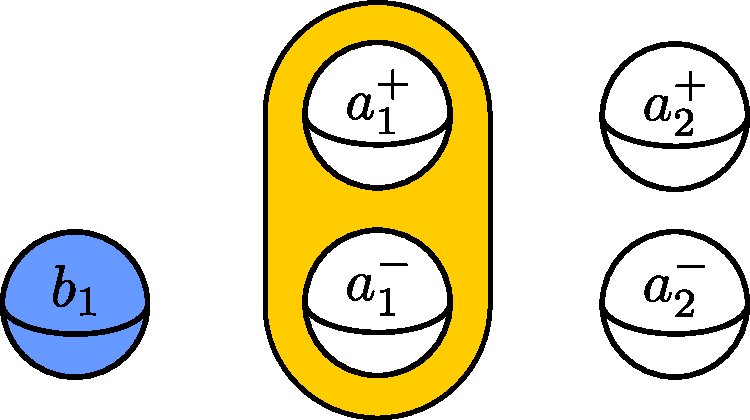
\includegraphics[width=\textwidth]{figures/sepconnect0.pdf}
        \caption{The basepoint sphere $v$ separates $a_1$
        from $a_2,\ldots, a_n$ and $b_1, \ldots, b_s$.}
        \label{fig:sepconnect0}
    \end{subfigure}
    ~
    \begin{subfigure}[t]{0.3\textwidth}
        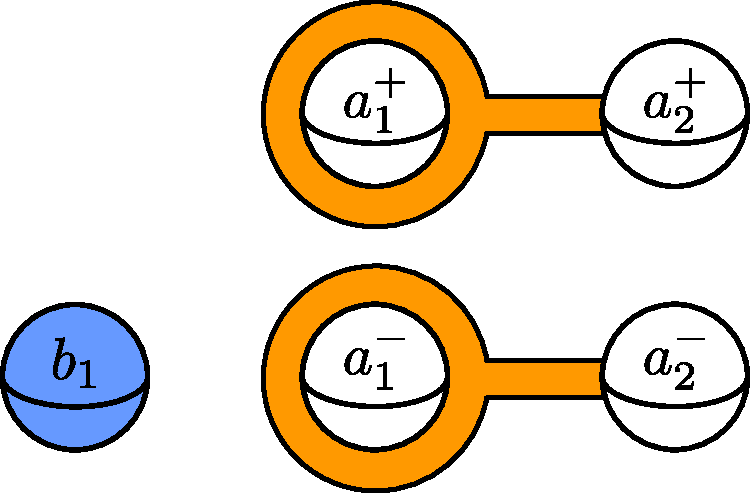
\includegraphics[width=\textwidth]{figures/sepconnect1.pdf}
        \caption{The transvection $a_1 \mapsto a_1a_2^{-1}$
        corresponds to
        pushing $a_1^+$ through $a_2^-$.}
        \label{fig:sepconnect1}
    \end{subfigure}
    ~
    \begin{subfigure}[t]{0.3\textwidth}
        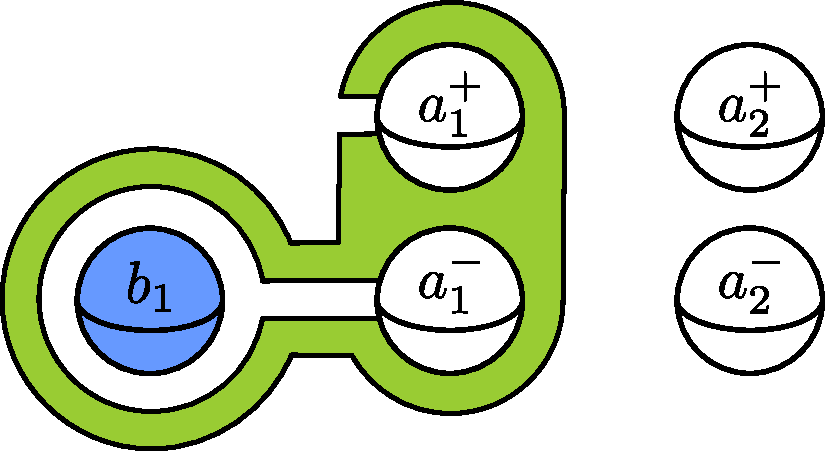
\includegraphics[width=\textwidth]{figures/sepconnect2.pdf}
        \caption{The conjugation $b_1 \mapsto a_1b_1a_1^{-1}$
        corresponds to pushing
        $b_1$ through $a_1^+$.}
        \label{fig:sepconnect2}
    \end{subfigure}
    \caption{Nontrivial $\oout_{n,p}$ generator actions on the base sphere $v$
    move $v$ at most distance 2 in $\mathcal S^{sep}_{n,p}$.}
    \label{sepconnect}
\end{figure}


Then $v'$ and $v$ are contained in a copy of $M_{1,2}$ bounded by $b_1$
and the sphere $u$ separating $a_1$ and $b_1$ from
$a_2, \ldots, a_n$ and $b_2, \ldots, b_s$.
If $n\geq 2$ or $p\geq 3$ we have that $u$
is essential and this gives a length 2 path $v$ to $u$ to $v'$ in $\mathcal {S}^{sep}_{n,p}$.
The inverse conjugation $b_1 \mapsto a_1^{-1}b_1a_1$ similarly
moves $v$ distance 2 in $\mathcal {S}^{sep}_{n,p}$.
Appealing to Putman's Lemma \ref{lemma:putman}, we conclude that
$\mathcal {S}^{sep}_{n,p}$ is connected for $n=1$ and $p\geq 3$.

Suppose $n \geq 2$.
Then generation of $\oout_{n,p}$ also requires transvection.
Consider the image $v'$ of $v$ under the
diffeomorphism corresponding to
the transvection $a_1 \mapsto a_1a_2^{-1}$,
as shown in orange in Figure \ref{sepconnect}.
Then $v'$ and $v$ are contained in a copy of $M_{2,1}$ bounded by
the sphere $u$ separating $a_1$ and $a_2$ from
$a_3, \ldots, a_n$ and $b_1, \ldots, b_s$.
If $n\geq 3$ or $p\geq 2$ we have that $u$
is essential and this gives a length 2 path $v$ to $u$ to $v'$ in $\mathcal {S}^{sep}_{n,p}$.
The inverse transvection $b_1 \mapsto a_1a_2$ similarly
moves $v$ distance 2 in $\mathcal {S}^{sep}_{n,p}$.
Appealing to Putman's Lemma \ref{lemma:putman}, we conclude that
$\mathcal {S}^{sep}_{n,p}$ is connected for $n=2$ and $p\geq 2$ or $n\geq 3$.




Finally, we show that $\mathcal {S}^{sep}_{2,1}$
is disconnected.
By capping the boundary component with a sphere we obtain a map
$$
\phi: \left (\mathcal {S}^{sep}_{2,1} \right )^{(0)} \to \left (\mathcal {S}^{sep}_{2,0} \right )^{(0)}
$$
Observe that if $u$ and $v$ are disjoint spheres of $\mathcal {S}^{sep}_{2,1}$
then $\phi(u)=\phi(v)$.
So $\phi$ gives a surjective simplicial map
$$
\mathcal {S}^{sep}_{2,1}  \to \mathcal {S}^{sep}_{2,0}.
$$
But as $\mathcal {S}^{sep}_{2,0}$ is totally disconnected it must be that ${S}^{sep}_{2,1}$
is disconnected.
\end{proof}


\noindent
We say that a sphere is $M_{n',p'}$-bounding if it bounds an embedded copy of $M_{n',p'} \subset M_{n,p}$.

\begin{lemma}
  \label{sepgenpreserved}
For $k\leq n/2$,
$M_{k,1}$-bounding spheres are characteristic in $\mathcal {S}^{sep}_{n}$ for $n\geq 3$.
\end{lemma}
\begin{proof}
Suppose that $x \in \mathcal {S}^{sep}_{n}$ bounds
an $M_{k,1}$.
Observe the link of $x$ is isomorphic to
a join
$\mathcal S^{sep}_{k,1}  \ast \mathcal S^{sep}_{n-k,1}$.
By Lemma \ref{sepflagdim}
the dimensions of the sides of the join are $2k-3$ and $2n-2k-3$,
so any automorphism of $\mathcal {S}^{sep}_{n}$
must send $x$ to a genus $k$-bounding sphere.
\end{proof}


Observe that
$M_{1,0} = S_1 \times S_2$
so that $\pi_2(M_{1,0},p) \cong \Z$.
Using the long exact sequence of the pair
$(M_{1,1},\partial M_{1,1})$
we compute  $\pi_2(M_{1,0}) \cong \pi_2 (M_{1,1}, S^2 )$,
so $M_{1,1}$
contains a unique homotopy class of nonseparating sphere
generating the second homotopy group.

Then for any automorphism $\phi \in \aaut \left (  \mathcal S^{sep}_{n,p}\right)$
we can extend $\phi$ to a map
$\hat \phi : \mathcal S_{n,p} \to \mathcal S_{n,p}$.
If $x$ is a separating sphere we assign $\hat \phi (x) = \phi(x)$.
If $a$ is a nonseparating sphere, then
there is there is an $M_{1,1}$-bounding sphere $x$
bounding an $M_{1,1}$ that contains $a$.
Then $\phi(x)$ bounds an $M_{1,1}$ by
Lemma \ref{sepgenpreserved}.
We define $\hat \phi(a)$ to be
the nonseparating sphere in the $M_{1,1}$ bounded by $\phi(x)$.
We must first demonstrate that $\hat \phi$ is well defined.

Fix a nonseparating sphere $a$.
Define a \emph{sharing pair} $\{x,x'\}$ (sharing $a$) to be
$M_{1,1}$-bounding spheres $x$ and $x'$
such that $x$ and $x'$ each bound an $M_{1,1}$ containing $a$
and are contained in a common $M_{2,1}$ bounded by separating sphere $y$.

\begin{lemma}
  \label{sepsharepair}
If $\{x,x'\}$ is a sharing pair, then $\{\phi(x),\phi(x')\}$
is a sharing pair for any
automorphism $\phi \in \aaut\left( \mathcal S^{sep}_{n} \right )$.
\end{lemma}

\begin{proof}
Let $a_1$ be a nonseparating sphere of $M_{n,p}$
and let $\{x,x'\}$ be a sharing pair for $a_1$.
Then $x$ and $x'$ are adjacent to an $M_{2,1}$-bounding sphere $y$,
but not each other in $\mathcal S^{sep}_{n}$.
Let $a_2$ be a nonseparating sphere disjoint from $a_1$ in the $M_{2,1}$ bounded by $y$.
Observe further we may find an $M_{1,1}$-bounding sphere
$z$ that intersects $y$, but not $x$ or $x'$.
\begin{figure}
% \floatbox[{\capbeside\thisfloatsetup{capbesideposition={right,top},capbesidewidth=.4\textwidth}}]{figure}[\FBwidth]
% {
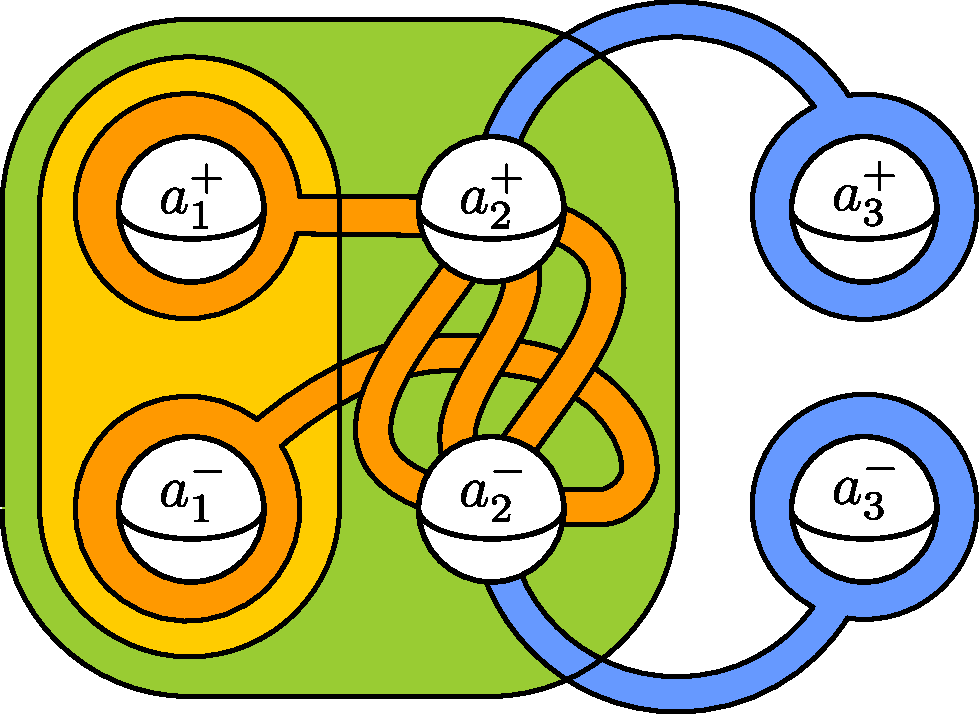
\includegraphics[width=.6\textwidth]{figures/sepsharepair.pdf}
\caption{
The sharing pair $x$ and $x'$ bound $M_{1,1}$ shown in yellow and orange.
They are contained in the green $M_{2,1}$ bounded by $y$.
The blue $M_{1,1}$ is bounded by $z$.
Observe an $M_{1,1}$-bounding sphere containing $a_1$ can be represented
by drawing two parallel copies $a^+_1$ and $a^-_1$ and then connecting them
by attaching a handle given by the regular neighborhood of an arc from $a_1^-$ to $a^+_1$ disjoint from $a_1$.
Fixing $a_1$, the spheres $x$ and $x'$ are determined by their respective intersection numbers with $a_2$.
}
\label{sepshare}
\end{figure}
Then, appealing to Lemma \ref{sepsharepair}, $\phi(x)$ and $\phi(x')$
must be intersecting $M_{1,1}$-bounding spheres.
Let $A$ be the $M_{2,1}$ bounded by $\phi(y)$.
$\phi(z)$ is disjoint from $\phi(x)$ and $\phi(x')$, but not $\phi(y)$.
Consider the image of $\phi(z)$ in the $A$.
If $\phi(z)$ bounded a region containing a nonseparating sphere in
$A$, there would only be one class of separating sphere in $A$
disjoint from $\phi(z)$.
Then $\phi(z)$  must bound in $A$
a handle given by the boundary of a regular neighborhood of an arc of
$\pi_1(A,\partial A)$ that must pass through a nonseparating sphere $a$ of $A$.
But then $\phi(x)$ and $\phi(x')$ must both bound the nonseparating sphere of $A$ disjoint from $a$.
So $\{\phi(x),\phi(x')\}$ is a sharing pair.
\end{proof}

Let $a$ be a nonseparating sphere of $M_n$.
We will show that any two $M_{1,1}$-bounding spheres
that contain $a$ on their $M_{1,1}$-side are connected by a sequence of
sharing pairs.
Let $\mathcal P_a$ be the \emph{sharing pair} graph defined as follows.
The vertices of $\mathcal P_a$
are genus 1-bounding separating spheres of $M_n$ that
bound an $M_{1,1}$ containing $a$.
Two vertices of $\mathcal P_a$ are adjacent
if they form a sharing pair for $a$.

\begin{lemma}
  \label{seppairgraph}
The sharing pair graph $\mathcal P_a$ is connected.
\end{lemma}

\begin{proof}
We appeal to Putman's Lemma \ref{lemma:putman}
using the graph $X=\mathcal P_a$ and the group
$G \leq \oout_{n}$ fixing $a$ setwise.
Let $a_1, \ldots, a_n$ be a basis for $F_n$.
Then $G$ is generated by
diffeomorphisms corresponding to
permutations of $\{a_2, \ldots, a_n\}$,
inversions, and the transvections
$a_1 \mapsto a_1a^{-1}_2$ and $a_2 \mapsto a_2a^{-1}_3$.

Observe that $G$ acts transitively on
$M_{1,1}$-bounding spheres
that contain $a$ on their genus 1-side.
Let $v$ be the sphere separating
$a_1$ from $a_2, \ldots, a_n$.
Observe that of the chosen generators only
the transvection $\phi: a_1 \mapsto a_1a^{-1}_2$
has nontrivial action on $v$.
But, as can be seen in figure \ref{sepconnect},
 $v$ and $\phi(v)$
 are contained in an $M_{2,1}$
 so that  $\{ v, \phi(v) \}$ is a sharing pair.

 It follow by Putman's Lemma \ref{lemma:putman} that $\mathcal P_a$ is connected.
\end{proof}

The previous Lemma shows that $\hat \phi$ is well defined.
If $a$ is a nonseparating sphere of $M_n$
and $x$ and $x'$ $M_{1,1}$-bounding sphere bounding an $M_{1,1}$ containing $a$,
then as $P_a$ is connected there is a sequence of sharing pairs from $x$ to $x'$.
By Lemma \ref{sepsharepair} this gives a sequence of
sharing pairs from $\phi(x)$ to $\phi(x')$.
But then $\phi(x)$ and $\phi(x')$ share the same nonseparating sphere
so that $\hat \phi (a)$ is well defined.

Certainly $\hat \phi$ is simplicial.
If $a$ and $a'$ are disjoint nonseparating spheres
then there are disjoint $M_{1,1}$-bounding spheres $x$ and $x'$ bounding
disjoint copies of $M_{1,1}$ separating $a$ and $a'$, respectively.
Since $\phi(x)$ and $\phi(x')$ are disjoint $M_{1,1}$-bounding spheres,
$\hat \phi(a)$ and $\hat \phi(a')$ are also disjoint.
If $y$ is a separating sphere disjoint from $a$, then
either there is an $M_{1,1}$-bounding sphere separating $a$ from $y$
or $y$ is an $M_{1,1}$-bounding sphere, so that $\hat \phi(a)$ is disjoint from $\hat \phi (y) = \phi(y)$.


% \thmsepspheres*

\begin{proof}[Proof of Theorem \ref{thm:sep}.]
The map constructed above
$$\Phi: \aaut \left ( \mathcal S^{sep}_n \right) \to \aaut \left ( \mathcal S_n \right)$$
with $\phi \mapsto \hat \phi$
is an isomorphism with the  map simply restricting automorphisms
$$\aaut \left ( \mathcal S_n \right) \to   \aaut \left ( \mathcal S^{sep}_n \right)$$
giving an inverse to $\Phi$.
Then the result follows from
Theorem \ref{aramsouto}.
\end{proof}

\section{Complexes of High Genus Separating Spheres}
\label{section:highgenussep}

For $k\leq n/2$, we call a sphere $x: S^2 \hookrightarrow M_{n,p}$ $k$-separating
if both components of
$M_{n,p}-x$
contain either a boundary component
or at least $k$ disjoint separating spheres.
If $x$ bounds a copy of $M_{j,1}$ with $j<n/2$,
we refer to it as to as $x^{in}$, or the \emph{inside} of $x$.
We will also describe objects disjoint from and inside of $x$ as \emph{engulfed} by $x$,
and disjoint objects on the outside as \emph{exgulfed} by $x$.

Let $\mathcal S^{sep,k}_{n,p} \subset \mathcal S^{sep}_{n,p}$
be the subcomplex spanned by homotopy classes of essential $k$-separating
spheres.
In this section we show that $\mathcal S^{sep,k}_{n,p}$ is a combinatorial model for $\oout_{n,p}$.

\thmhighsep*

Observe that for $k>1$,
$\mathcal S^{sep,k}_{n,p}$
does not have a uniform dimension.
For example, in the case with no boundary components, $p=0$,
we can construct
a maximal (with respect to inclusion)
simplex of maximal dimension
\hbox{$n-2k$}
as in Figure \ref{bigsimp}.
\begin{figure}[b!]
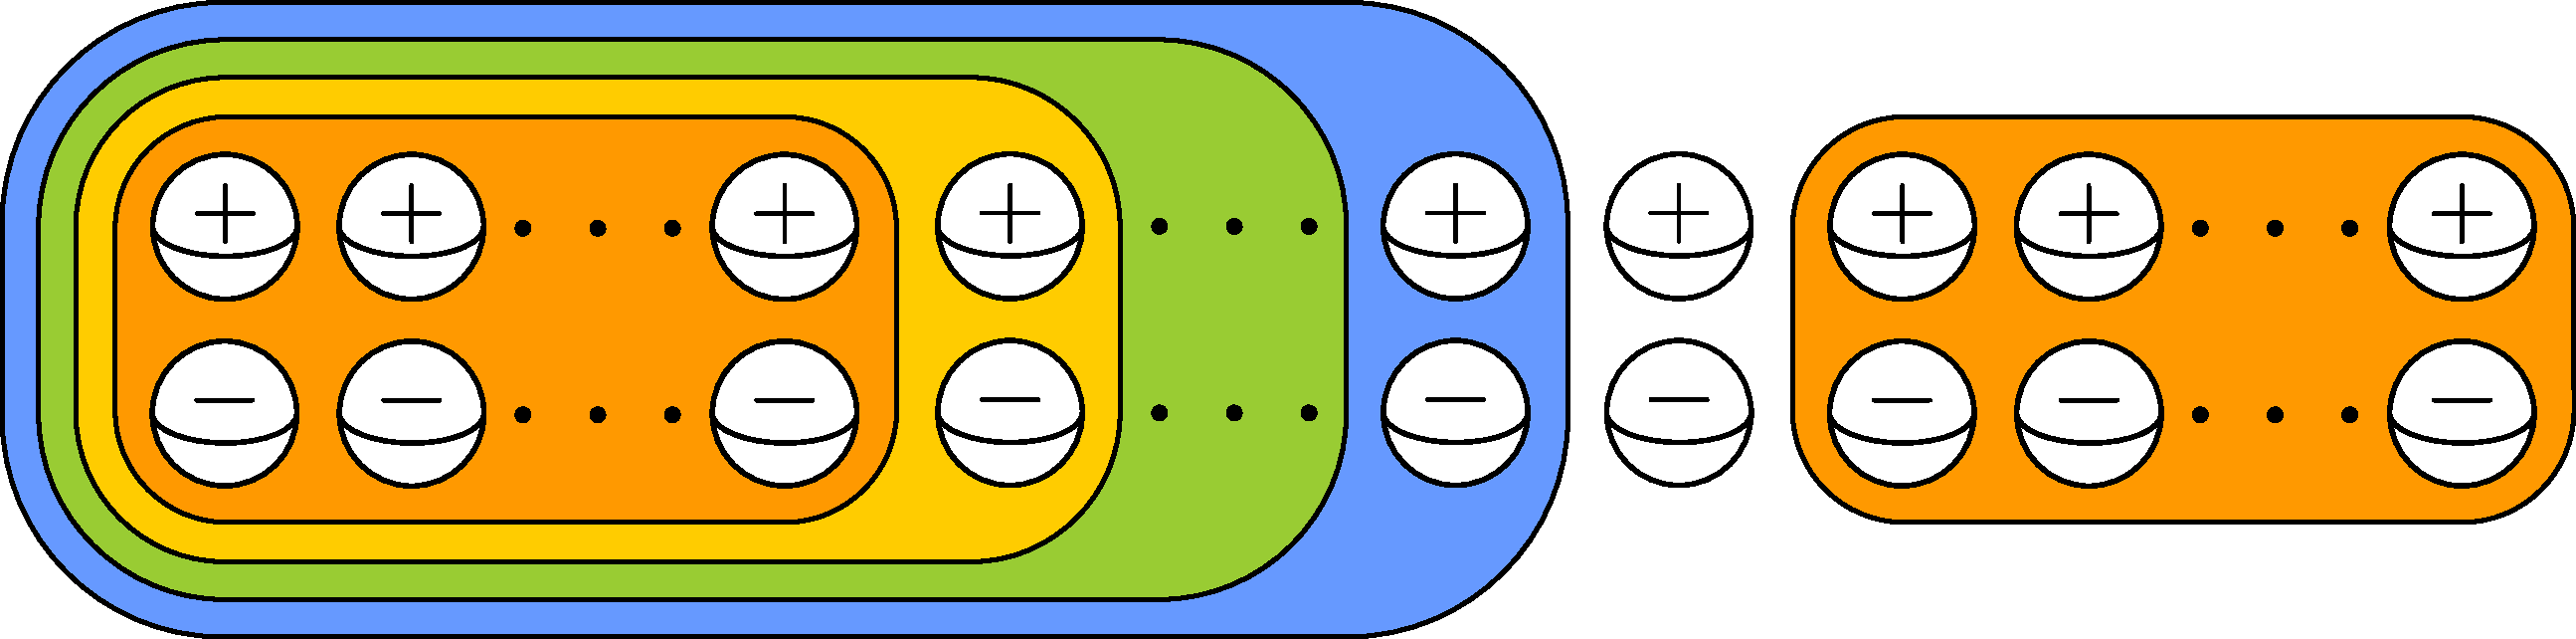
\includegraphics[width=\textwidth]{figures/bigsimplex.pdf}
\caption{A maximal dimension maximal simplex of $\mathcal S^{sep,k}_{n}$ for $k>1$
is spanned by $n-2k+1$ spheres and cuts $M_n$ into 2 copies of $M_{k,1}$ and $n-2k$
copies of $M_{1,2}$.
The corresponding graph of $M_{n}$ components is an unbranched tree
with 2 leaves of weight $k$ and $n-2k$ internal vertices of weight 1.}
\label{bigsimp}
\end{figure}
If we write $n=qk+r$ with $q = \lfloor n/k \rfloor$ and $0<r<k$,
then we can construct maximal (with respect to inclusion) simplices
of smaller dimension $2q+r-4$ as in Figure \ref{lilsimp}.
\begin{figure}[b!]
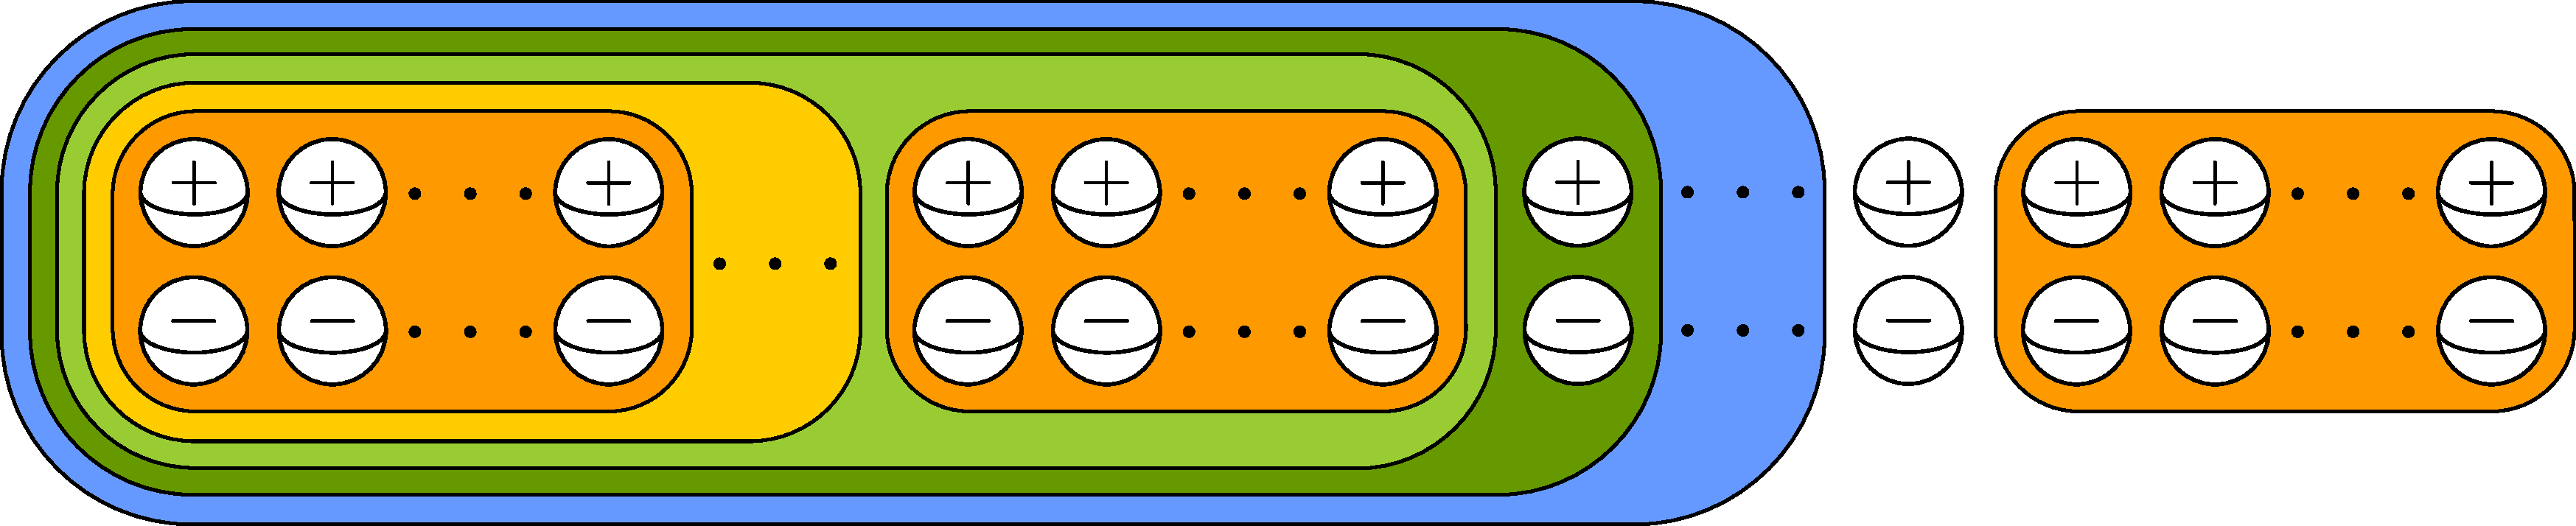
\includegraphics[width=\textwidth]{figures/smallersimplex.pdf}
\caption{A minimal dimension maximal simplex of $\mathcal S^{sep,k}_{n}$ for $k>1$
is spanned by $2q+r-3$ spheres and cuts $M_n$
into $q$ copies of $M_{k,1}$ and $r$ copies of $M_{1,2}$ and $q-2$ copies of $M_{0,3}$.
The corresponding graph of $M_{n}$ components is a tree
with $q$ leaves of weight $k$ and $q-2$ internal vertices weight 0
and $r$ internal vertices of weight 1.}
\label{lilsimp}
\end{figure}

If there are boundary spheres we can construct a maximal dimension simplex
similar to Figure \ref{bigsimp}
by replacing the $M_{k,1}$-bounding spheres with boundary spheres.
Similar linear nesting shows any $k$-separating sphere can be contained in a maximum dimension simplex
of dimension for $k>1$
$$
\max_n \left \{
\Delta^n \hookrightarrow
\mathcal S^{sep,k}_{n,p}
\right \}
=
\begin{cases}
  n-2k & \mbox{ if } p=0\\
  n-k & \mbox{ if } p=1\\
  n+p-3 & \mbox{ if } s\geq 2
\end{cases}.
$$

\begin{lemma}
  \label{ksepconnect}
For $1<k<n/2$,
the complex of $k$-separating spheres
$\mathcal S^{sep,k}_{n,p}$
is connected whenever it has positive dimensional simplices if $p=0$,
and whenever it has 2 dimensional simplices if $p>0$.
\end{lemma}

\begin{proof}
The proof is by Putman's Lemma \ref{lemma:putman}
with the group $\oout_{n,p}$.

Consider first the case with $p=0$
and suppose that $\mathcal S^{sep,k}_{n,p}$ has positive dimensional simplices.
So $n>2k$, and in particular
there are $M_{k,1}$ and $M_{k+1,1}$-bounding spheres in $\mathcal S^{sep,k}_{n,p}$.
Choose a sphere $v$ to be an $M_{k,1}$-bounding sphere.
Observe that every $k$-separating sphere is disjoint from a
$M_{k,1}$-bounding sphere, and the $M_{k,1}$-bounding spheres
are exactly the $\oout_{n}$ orbit of $v$.
Let $a_1,\ldots,a_n$ be a maximal collection of disjoint nonseparating spheres
of $M_{n}$ with $a_1,\ldots, a_k$ engulfed by $v$.
Consider as a generating set for $\oout_{n}$
the transpositions and inversions of $a_1,\ldots,a_n$
and the transposition diffeomorphism $t$ corresponding to $a_1 \mapsto a_1a_{k+1}^{-1}$.
Observe that every inversion fixes $v$.
Observe that a transposition $\phi$ either fixes $v$, in the case it swaps
spheres on the same side of $M_n-v$, or $\phi(v)$ and $v$ are contained in a common
$M_{k+1,1}$-bounding sphere that is $k$-separating, as in Figure
\ref{fig:kput0}.
Finally, $v$ and $t(v)$ are contained in a common
$M_{k+1,1}$-bounding sphere as in Figure \ref{fig:kput1}.
The connectivity then follows by Putnam's Lemma.
\begin{figure}[b!]
    \centering
    \begin{subfigure}[b]{0.4\textwidth}
        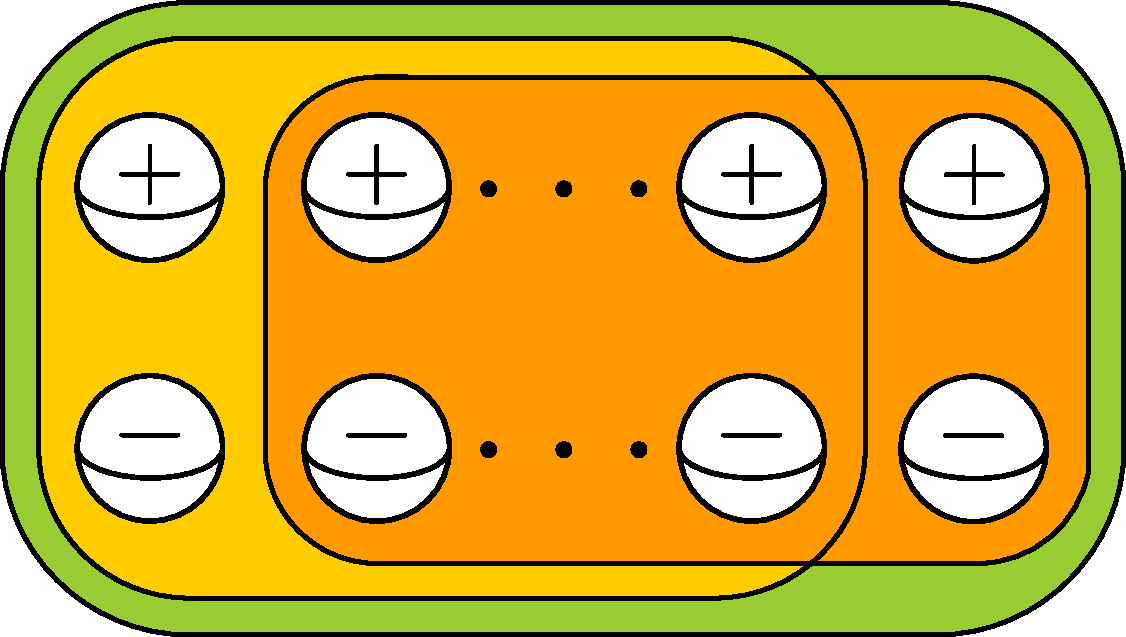
\includegraphics[width=\textwidth]{figures/kput0.pdf}
        \caption{Transpositions move $M_{k,1}$-bounding spheres distance 2.}
        \label{fig:kput0}
    \end{subfigure}
    ~
    \begin{subfigure}[b]{0.4\textwidth}
        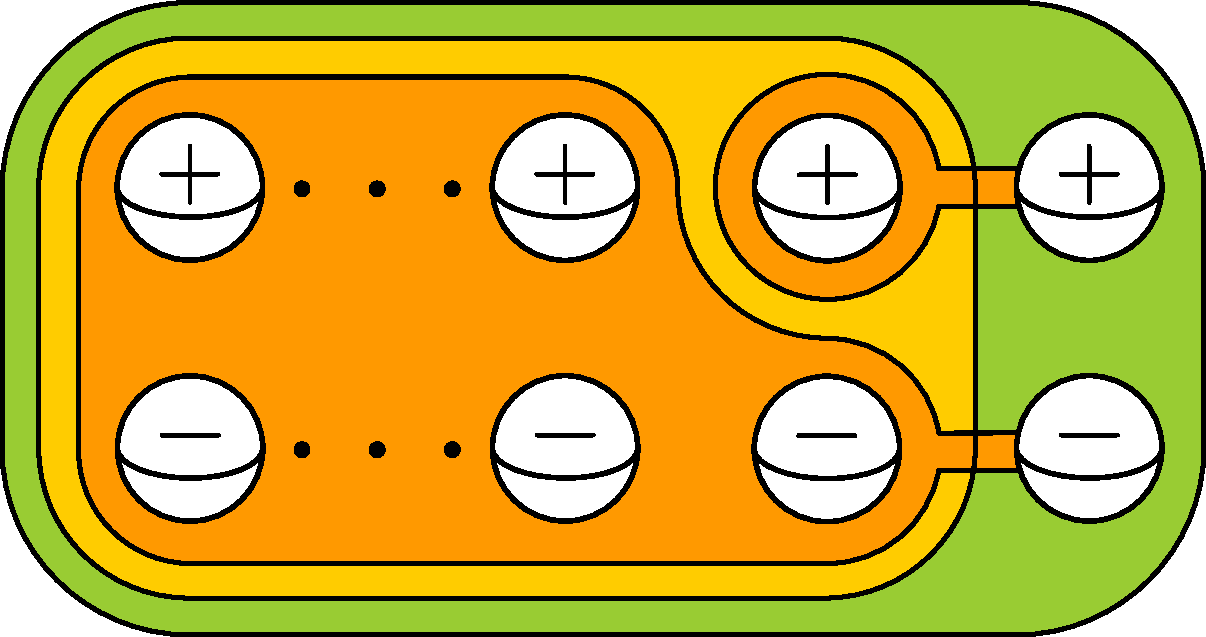
\includegraphics[width=\textwidth]{figures/kput1.pdf}
        \caption{Transvections move $M_{k,1}$-bounding spheres distance 2.}
        \label{fig:kput1}
    \end{subfigure}
    \caption{Nontrivial $\oout_{n}$ generator actions on the base sphere $v$
    move $v$ at most distance 2 in $\mathcal S^{sep,k}_{n,p}$.}
    \label{fig:kput01}
\end{figure}

Consider the case with $p>0$.
If
$p=1$
then to have dimension 2 simplices $n \geq k+2$,
and $M_{2,2}$-bounding spheres are $k$-separating.
If
$p>1$
then to have dimension 2 simplices $n+p\geq 5$.
If $p=1$ then $n \geq 4$
so that $M_{2,2}$-bounding spheres are disjoint from a
$M_{k,1}$-bounding sphere and must be $k$-separating.
If $p>1$ then $n \geq 4$
so that $M_{1,3}$ and $M_{2,2}$-bounding spheres are disjoint from a
$M_{1,2}$ or $M_{k,1}$-bounding sphere and must be $k$-separating.


Choose a sphere $v$ to be an $M_{1,2}$-bounding sphere.
Observe that every $k$-separating sphere is disjoint from a
$M_{1,2}$-bounding sphere, and the $M_{1,2}$-bounding spheres
are exactly the $\oout_{n,p}$ orbit of $v$.
Let $b_1,\ldots,b_s$ be the bounding spheres
and let $a_1$ be a nonseparating sphere engulfed by $v$ and $a_2, \ldots, a_n$
disjoint nonseparating spheres disjoint from $v$ and $a_1$.
Consider as a generating set for $\oout_{n,p}$
diffeomorphisms corresponding to
transpositions of $a_1,\ldots,a_n$,
transpositions of $b_1,\ldots,b_s$,
$t$ the transvection $a_1 \mapsto a_1a_2^{-1}$,
and $u$ the $b_1$ push corresponding to
conjugation $b_1 \mapsto a_1b_1a_1^{-1}$.
Observe first that $u$ leaves $v$ fixed.
Observe  that $\phi$ a
transposition of  $a_1,\ldots,a_n$
either leaves $v$ if it fixes $a_1$, or
swaps $a_1$, and then $\phi(v)$ and $v$
are engulfed by an $M_{2,2}$-bounding sphere as in Figure \ref{fig:kput2}.
Observe that $\psi$ a
transposition of  $b_1,\ldots,b_s$
either leaves $v$ if it fixes $b_1$, or
swaps $b_1$, and then $\psi(v)$ and $v$
are engulfed by an $M_{1,3}$-bounding sphere as in Figure \ref{fig:kput3}.
Finally,
$v$ and $t(v)$
are engulfed by an $M_{2,2}$-bounding sphere as in Figure \ref{fig:kput4}.
The connectivity then follows by Putnam's Lemma.
\begin{figure}[b!]
    \centering
    \begin{subfigure}[b]{0.3\textwidth}
        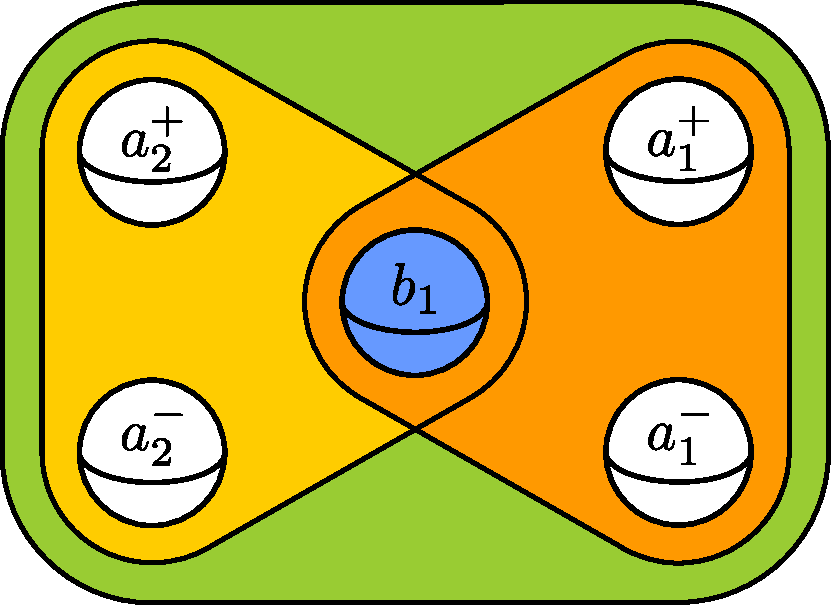
\includegraphics[width=\textwidth]{figures/kput2.pdf}
        \caption{$a$-Transposition}
        \label{fig:kput2}
    \end{subfigure}
    ~
    \begin{subfigure}[b]{0.3\textwidth}
        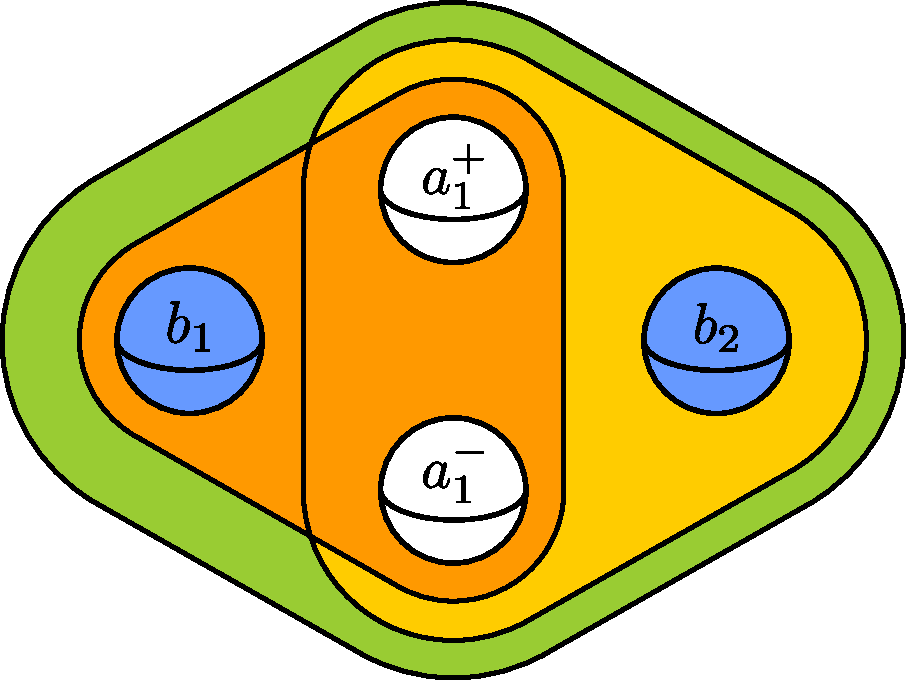
\includegraphics[width=\textwidth]{figures/kput3.pdf}
        \caption{$b$-Transposition}
        \label{fig:kput3}
    \end{subfigure}
    ~ %add desired spacing between images, e. g. ~, \quad, \qquad, \hfill etc.
      %(or a blank line to force the subfigure onto a new line)
    \begin{subfigure}[b]{0.3\textwidth}
        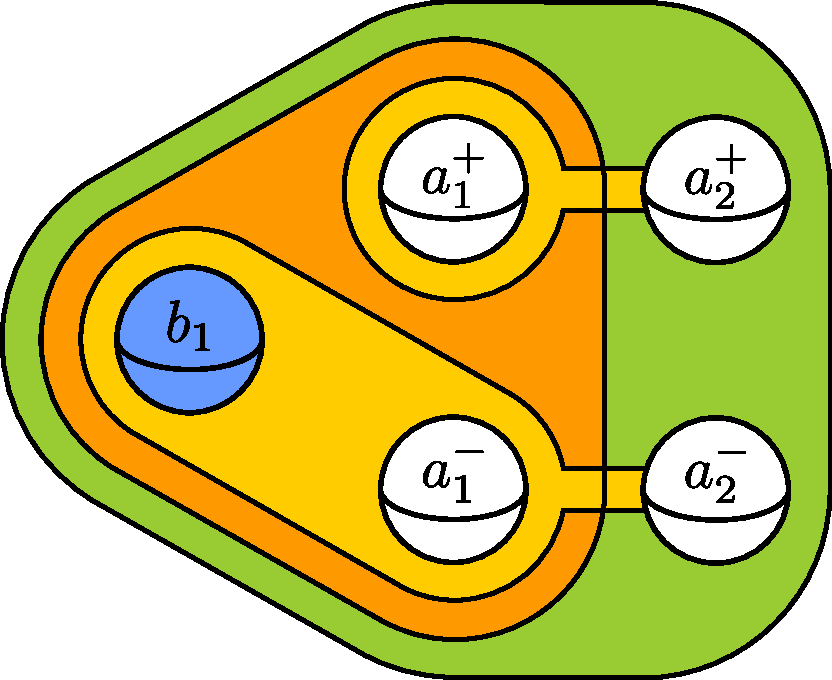
\includegraphics[width=\textwidth]{figures/kput4.pdf}
        \caption{Transvection}
        \label{fig:kput4}
    \end{subfigure}
    \caption{Nontrivial $\oout_{n,p}$ generator actions on the
    base sphere $v$ move $v$ at most distance 2
    in $\mathcal S^{sep,k}_{n,p}$.}
    \label{fig:kput234}
\end{figure}
\end{proof}

\begin{lemma}
Let $n\geq 3$ and $\phi \in \aaut{ \left ( \mathcal S^{sep,k}_{n} \right ) }$.
For $n/2>j\geq k$,
if $x$ is a
$M_{j,1}$-bounding spheres
engulfing a sphere $y$,
then $\phi(x)$
is a
$M_{j,1}$-bounding spheres
engulfing the sphere $\phi(y)$.
\label{kengulfschar}
\end{lemma}

\begin{proof}
  Suppose that $x$ bounds an $M_{j,1}$ in $\mathcal S^{sep,k}_{n}$.
  Consider the subcomplex
  $\mathcal E_x$ spanned by spheres engulfed by $x$
  and the subcomplex
  $\mathcal F_x$ spanned by spheres disjoint but not engulfed by $x$.
  The link of $x$ is a join $\mathcal E_x \ast \mathcal F_x$
  and
  $\mathcal E_x \cong \mathcal S^{sep,k}_{j,1}$
  and $\mathcal F_x \cong \mathcal S^{sep,k}_{n-j,1}$.
  Then according to Lemma \ref{ksepconnect},
  $\mathcal E_x$
  and $\mathcal F_x$
  have simplices with maximal dimension
  $j-k$ and $n-j-k$, respectively.
  So the link of $\phi(x)$ must have the same structure
  and $\phi(x)$ must be $M_{j,1}$-bounding.
  Note that since
  $$\phi \left( \mathcal E_x \right) =\mathcal E_{\phi(x)}$$
  any sphere $y$ engulfed by $x$ has $\phi(y)$ engulfed by $\phi(x)$.
\end{proof}

We hope to extend automorphisms of
$\mathcal S^{sep,k}_{n}$ to
automorphisms of $\mathcal S^{sep,k-1}_{n}$
by
a
combinatorial characterization of
$M_{k-1,1}$-bounding spheres in $\mathcal S^{sep,k}_{n}$.

This is the direct analog of handle pairs of Brendle-Margalit \cite{meta}.

\begin{definition}
  If $x$ is an $M_{k,1}$-bounding sphere engulfed by $M_{k+1,1}$-bounding sphere $y$
  we say that a pair $v,w$ of $M_{k,1}$-bounding spheres
  \emph{carve} $x$ from $y$ if
  \begin{enumerate}[(1)]
    \item Each pair of $v,w,y$ intersects, but $v,w,y$ are all disjoint from $x$.
    $$
    \begin{tikzcd}[every arrow/.append style={dash}]
      v \arrow{r} & x \arrow{r} & y\\
      w \arrow{ur} &&
    \end{tikzcd}
    $$
    \item The $M_{k,1}$-bounding sphere $x$ is the unique sphere engulfed by $y$
    and disjoint from both $v$ and $w$.
    \item There is more than one $M_{k,1}$-bounding sphere engulfed by $y$ and disjoint
    from $v$ but not $w$.
    \item There is more than one $M_{k,1}$-bounding sphere engulfed by $y$ and disjoint
    from $w$ but not $v$.
  \end{enumerate}
\end{definition}

It follows immediately from this combinatorial definition and
Lemma \ref{kengulfschar} that carving is characteristic.
The following Lemma shows additionally that there is
a unique nonseparating sphere that was
``carved away'' from $y$.


\begin{lemma}
  Let $\phi \in \aaut \mathcal S^{sep,k}_{n}$.
  If $v,w$ carve $x$ from $y$,
  then
  \begin{enumerate}[(1)]
  \item $\phi(v), \phi(w)$ carve $\phi(x)$ from $\phi(y)$
  \item One of the spheres $v$ or $w$
  contains a disk or annulus $p$ with $\partial s \subset y$ whose image in $y^{in}/y$
  is homotopic to a nonseparating sphere.
  \item There is an arc $\alpha$ with endpoints on $y$
  such that $v$ and $w$ separate $\alpha$ from $x$.
  \item $x$ is the unique $M_{k,1}$-bounding sphere engulfed by $y$ and disjoint from $p$ and $\alpha$.
\end{enumerate}
\label{carvingchar}
\end{lemma}

\begin{proof}
  (1) follows from Lemma \ref{kengulfschar} and the combinatorial definition of carving.\\
  (2) Fix representatives for $v$, $w$, $x$, and $y$ that intersect minimally and transversely.
  Then $w\cap y^{in}$ is a collection of disks and annuli with boundary on $y$.
  No component disk or annulus of $w\cap y^{in}$ can be separating,
  or else there would be at most $M_{k,1}$ in $y^{in}$
  disjoint from $w$.
  Similarly $v\cap y^{in}$ is a collection of disks and annuli, no one of that separates $y^{in}$.
  Let $\beta$ be any nontrivial loop in $y^{in}-x^{in}$ and based at
  a point on $x$.
  Then $\beta$ must intersect either $v$ or $w$, or else
  the pushes of any nonseparating sphere of $x$ about $\alpha$
  would yield infinitely many $M_{k,1}$-bounding spheres engulfed by $y$
  and disjoint from $v$ and $w$, contrary to the hypothesis.
  Since no such $\beta$ exists,
  there must a component $p$ of $v\cap y^{in}$ or $w\cap y^{in}$
  whose image in the quotient
  $y^{in}/y$ is homotopic to a nonseparating sphere.\\
  (3) Let $a$ be a nonseparating sphere engulfed by $y$ and exgulfed by $x$
  and disjoint from the nonseparating component $p$ as above.
  If $v\cap y^{in}$ or $w\cap y^{in}$
  have a component that intersects $a$, then as $v$ and $w$ are separating there
  must be an arc intersecting $a$ with endpoints on $y$ that they separate from $x$.
  Suppose that $v$ and $w$ are disjoint from $a$.
  If there is a loop $\gamma$ based at $a$ that winds through a noseparating sphere engulfed by $x$
  and is disjoint from $v$ and $w$,
  then the pushes of $a$ along $\gamma$ leave $v$ and $w$ unchanged,
  but the images of $x$ give infintely many $M_{k,1}$-bounding spheres
  engulfed by $y$ and disjoint from $v$ and $w$, in contradiction
  with the definiton of carving.
  Then $v$ and $w$ must separate $a$ from $x$ in $y$, and there is an
  arc $\alpha$ with end points on $y$ that intersects $a$ once and
  so must be separated from $x$ by $v$ and $w$.\\
  (4) Assume to the contrary there is some $x'$ engulfed by $y$,
   distinct from $x$,
   and disjoint from $p$ and $\alpha$.
   Then there must be some nonseparating sphere $a$ engulfed $x'$ but not $x$.
   Note that $y^{in}-x^{in} \cong M_{1,2}$
   and consider the components of $a \cap (y^{in}-x^{in})$.
   If $a \cap (y^{in}-x^{in})$ has a nonseparating disk,
   it must intersect $\alpha$.
   If $a \cap (y^{in}-x^{in})$ contains a nontrivial arc,
   it must intersect $p$. So $a$ must be engulfed by $x$.
\end{proof}

\begin{definition}
Define an $M_{k-1,1}$-sharing pair
 $\{x_0,x_1\}$
 to be a pair of $M_{k,1}$-bounding spheres $x_0,x_1 \in \mathcal S^{sep,k}_{n}$
such that:
\begin{enumerate}[(1)]
  \item
  There are $M_{k,1}$-bounding spheres $x_2,x_3$ and a
$M_{k+1,1}$-bounding sphere $y$
such that the induced subgraph of $\mathcal S^{sep,k}_{n}$
on $y,x_0,x_1,v_0,v_1,w_0,w_1$ is exactly
$$
\begin{tikzcd}[every arrow/.append style={dash}]
x_0 \arrow{d} \arrow{r} \arrow[bend right=60]{dd}& y \arrow{r}& x_1 \arrow{d} \arrow[bend left=60]{dd}\\
v_0 \arrow{rr} \arrow{rrd}&&  v_1\\
w_0 \arrow{rr} \arrow{rru} &&  w_1
\end{tikzcd}
$$
and
\item For $i=0,1$ the spheres $v_i,w_i$ carve $x_i$ from $y_i$.
\item For $z_0 \in \{v_0,w_0\}$ and $z_1 \in \{v_1,w_1\}$,
there is no $M_{k,1}$-bounding sphere engulfed by $y$ and disjoint from both
$z_0$ and $z_1$.
\end{enumerate}
\label{def:ksharepair}
\end{definition}


\begin{lemma}
  The spheres of an $M_{k-1,1}$-sharing pair
  uniquely engulf a
  $M_{k-1,1}$-bounding sphere in $M_n$.
\end{lemma}

\begin{proof}
Let $\{x_0,x_1\}$ be a sharing pair with $y,v_0,w_0,v_1,w_1$ as above.
Let $p_i$ and $\alpha_i$
be as specified in Lemma \ref{carvingchar},
so that,
without loss of generality,
$p_i$ is a component of $v_i \cap y^{in}$ that is nonseparating in $y$.
And $\alpha_i$ is a loop with endpoints on $y$ that $v_i$ and $w_i$ separate from $x_i$.
But as $v_0$ and $v_1$ are disjoint, so are $p_0$ and $p_1$.

Since there is no $M_{k,1}$-bounding sphere disjoint from
both $v_0$ and $v_1$, it must be no $M_{k-1,1}$-bounding sphere
is disjoint from both $p_0$ and $p_1$ or from both $\alpha_0$ and $\alpha_1$.

Then $\alpha_1$ must intersect $x_0$,
and there are $k-1$
disjoint nonseparting spheres $a_1,\ldots, a_{k-1}$
engulfed by $x$ and disjoint from $\alpha_1$.


Consider the images in $y^{in}/y \cong M_{k+1,1}$.
Then the images of $p_0$ and ${s_1}$
are distinct nonseparating spheres in $y^{in}/y$.
Further since there is no $M_{k,1}$-bounding sphere disjoint from
both, forgetting the basepoint $y/y$ in $y^{in}/y$
gives distinct, disjoint spheres
$\overline{s_0}$ and $\overline{s_1}$ of $y^{in}$.
Let $\Sigma$ be a system of $n-k-1$ disjoint spheres exgulfed by $y$.

The let $z$ be the unique sphere separating
$a_1,\ldots,a_k$ from $\overline{s_0}$, $\overline{s_1}$, and $\Sigma$.
Then $z$ is $M_{k-1,1}$-bounding and
uniquely engulfed by both $x_0$ and $x_1$.
\end{proof}


\begin{lemma}
  Sharing pairs are characteristic.\\
  If $\{x_0,x_1\}$ is an $M_{k-1,1}$-sharing pair with $x_0,x_1 \in \mathcal S^{sep,k}_n$
  and $\phi \in \aaut \mathcal S^{sep,k}_n$,
  then $\{\phi(x_0),\phi(x_1)\}$ is an $M_{k-1,1}$-sharing pair.
  \label{lemma:sharepreserve}
\end{lemma}

\begin{proof}
  Let $y,x_0,v_0,w_0,x_1,v_1,w_1$ be as in Definition \ref{def:ksharepair}.
  By Lemma \ref{kengulfschar} $\phi(x_0),\ldots, \phi(x_3)$
  are $M_{k,1}$-bounding and $\phi(y)$ is $M_{k+1,1}$-bounding.
  The $\phi$ image of the induced subgraph on $y,x_0,v_0,w_0,x_1,v_1,w_1$
  is an isomorphic graph.
  Property (2) is preserved by Lemma \ref{carvingchar}.
  Property (3) of Definition \ref{def:ksharepair}
  is preserved by its combinatorial definition.
\end{proof}

% Although the representation of $M_{k-1,1}$-bounding spheres
% are

\begin{remark}
  Every $M_{k-1,1}$-bounding sphere $x$ admits an $M_{k-1,1}$-sharing pair in
  $\mathcal S^{sep,k}_{n}$ engulfing $x$, provided $n\geq 3k$.
  By a change of coordinates the,
  arrangement in Figure \ref{fig:ksharing} shows a possible pair sharing $x$.

  \begin{figure}[h!]
  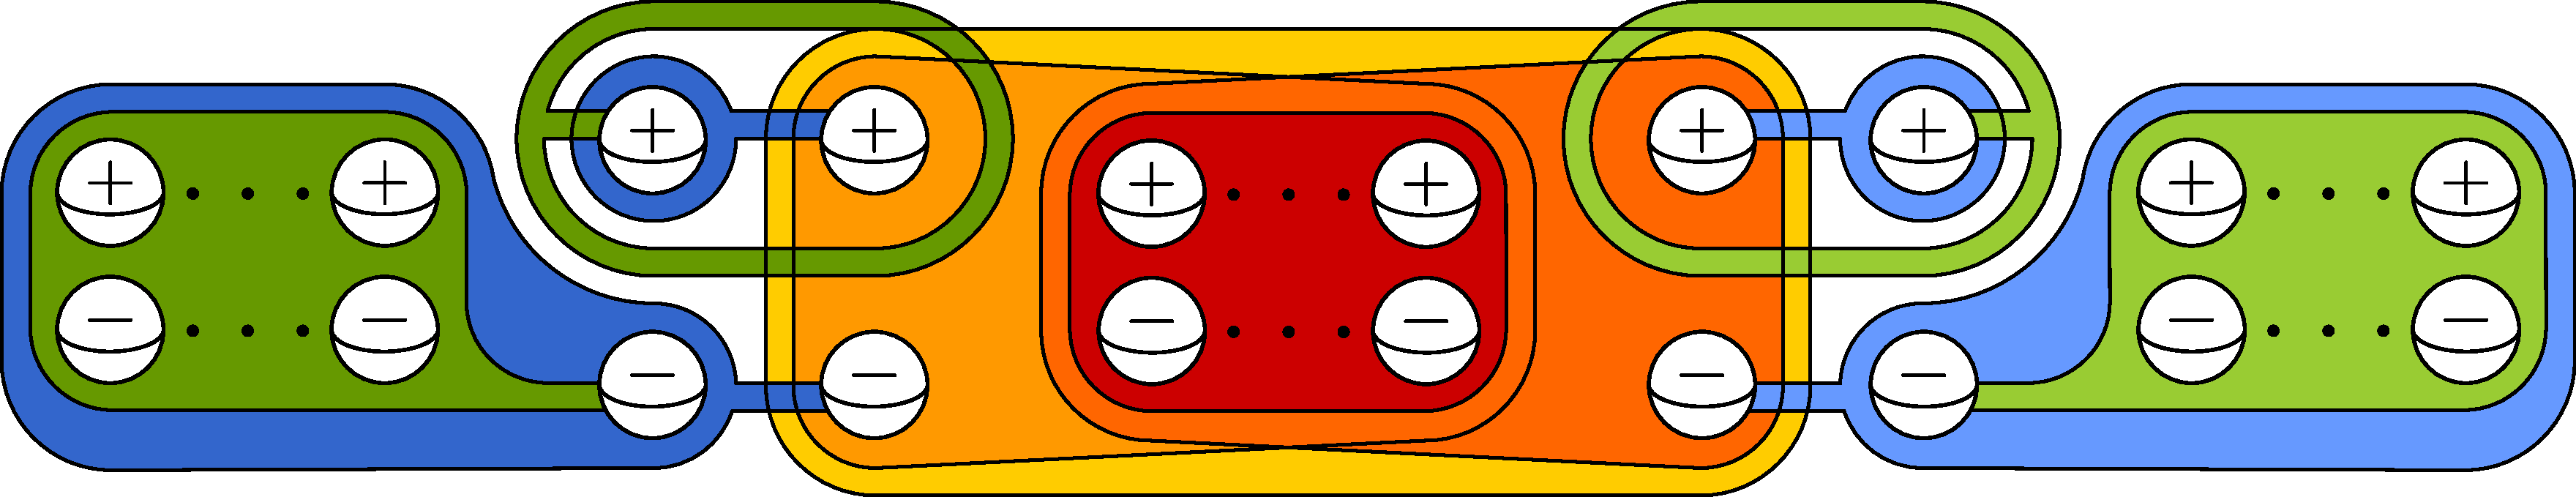
\includegraphics[width=\textwidth]{figures/ksharingnotpent.pdf}
  \caption{
    A sharing pair and the requisite carvings.
    The pair $\{x_0,x_1\}$ is shown bounding dark and light orange, respectively.
    The pair shares the $M_{k-1,1}$-bounding sphere $x$ shown bounding red.
    The pair is engulfed by $M_{k+1,1}$-bounding sphere $y$ shown in yellow.
    Dark orange $x_0$ is carved by $v_0$ and $w_0$ shown in dark green and blue.
    Light orange $x_1$ is carved by $v_1$ and $w_1$ shown in light green and blue.
  }
  \label{fig:ksharing}
  \end{figure}
\end{remark}


We call three spheres an $M_{k-1,1}$-sharing triple if
the spheres pairwise form sharing pairs and all engulf
a common $M_{k-1,1}$-bounding sphere.

\begin{lemma}
  Sharing triples are characteristic.\\
  If $\{x_0,x_1,x_2\}$ is an $M_{k-1,1}$-sharing triple with $x_0,x_1,x_2 \in \mathcal S^{sep,k}_n$
  and $\phi \in \aaut \mathcal S^{sep,k}_n$,
  then $\{\phi(x_0),\phi(x_1),\phi(x_2)\}$ is an $M_{k-1,1}$-sharing triple.
  \label{lemma:sharetrippreserve}
\end{lemma}

\begin{proof}
  According to Lemma \ref{lemma:sharepreserve}
  if $x_0,x_1,x_2$ pairwise form sharing pairs,
  then so do $\phi(x_0),\phi(x_1),\phi(x_2)$.
  It remains only to see that
  $\phi(x_0),\phi(x_1),\phi(x_2)$ all engulf a
  common $M_{k-1,1}$-bounding sphere, rather that a distinct
  $M_{k-1,1}$-bounding sphere for each pair.
  We reduce the proof to showing
  $\phi(x_0),\phi(x_1),\phi(x_2)$ all engulf a
  common $M_{k-1,1}$-bounding sphere if and only if there is
  no $M_{k+1,1}$-bounding sphere $y$ engulfing
  $\phi(x_0),\phi(x_1),$ and $\phi(x_2)$.
  Then if there were a $y$ engulfing $\phi(x_0),\phi(x_1),$ and $\phi(x_2)$, we would have
  $\phi^{-1}(y)$ engulfs $x_0,x_1,x_2$, which would contradict that
  $\{x_0,x_1,x_2\}$ is a sharing triple.

  Observe that, as in the proof of Lemma \ref{lemma:sharepreserve},
  since $\phi(x_0),\phi(x_1),\phi(x_2)$
  are pairwise sharing pairs,
  there are three pairwise-disjoint $M_{1,1}$-bounding spheres $z_0,z_1,z_2$
  such that $z_i$ is uniquely engulfed by $\phi(x_i)$ and disjoint
  but not engulfed by $\phi(x_{i+1})$, for $i \in \Z/3$.
  The sphere shared by $\{\phi(x_i),\phi(x_{i+1})\}$
  is in $\phi(x_i)^{in}-z_i^{in}$.
  If $\phi(x_0),\phi(x_1),\phi(x_2)$ all engulf a
  common $M_{k-1,1}$-bounding sphere $x$,
  then any sphere engulfing $\phi(x_0),\phi(x_1),\phi(x_2)$
  contains $x,z_0,z_1,$ and $z_2$ so must be $M_{j,1}$-bounding for $j\geq k+2$.
  If $\phi(x_0),\phi(x_1),\phi(x_2)$ do not engulf
  a common $M_{k-1,1}$-bounding sphere,
  then for $i \in \Z/3$
  we have a distinct $M_{k-1,1}$-bounding sphere
  shared by
  $\{\phi(x_i),\phi(x_{i+1})\}$ and that engulfs $z_{i-1}$.
  But then
  $\phi(x_0),\phi(x_1),\phi(x_2)$ do all engulf
  a common $M_{k-2,1}$-bounding sphere $x$
  such that $\phi(x_i)$ engulfs $x$ and $z_i$ and $z_{i+1}$.
  Then the same $M_{k+1,1}$-bounding sphere $y$ fits into the defining pentagon
  of Definition \ref{def:ksharepair}
  for all three sharing pairs.
\end{proof}

Let $x$ be an $M_{k-1,1}$-bounding sphere.
We will show that any two sharing pairs engulfing $x$
are connected by a sequence of sharing triples.
Let $\mathcal P_x$ be the \emph{sharing pair} graph defined as follows.
The vertices of $\mathcal P_x$ are $M_{k-1,1}$-sharing pairs in
$\mathcal S^{sep,k}_n$ engulfing
$x$, where $n\geq 3k$.
Two vertices $\{x_0,x_1\}$ and $\{x_1,x_2\}$
of $\mathcal P_x$ are adjacent if the pairs
have a common member and the three spheres
form an $M_{k-1,1}$-sharing triple engulfing $x$.

% By Lemma \ref{lemma:sharepreserve}, an automorphism
% $\phi \in \aaut \mathcal S^{sep,k}_n$
% induces an isomorphism
% $\mathcal P_x \stackrel{\cong}{\longrightarrow} \mathcal P_{\phi(x)}$
% .


\begin{lemma}
  The sharing pair graph $\mathcal P_x$ is connected for $n\geq 3k$ and $k\geq 2$.
  \label{lem:kshareconnect}
\end{lemma}

\begin{proof}
  We appeal to Putman's Lemma \ref{lemma:putman}.
  Fix an $M_{k-1,1}$-bounding sphere $x$ and
  an $M_{k-1,1}$-sharing pair $v=\{x_0,x_1\}$ engulfing $x$ with $x_0$ and $x_1$ having geometric intersection 1.
  Let $G \leq \oout_{n}$ be the subgroup fixing $x^{in}$, so that $G\cong \oout_{n-k+1,1}$.


  Observe that if two $x$-sharing pairs $\{x_0,x_1\}$ and $\{x_1,x_2\}$
  contain a common member $x_1$ and with all three spheres engulfed
  by a common $M_{k+1,1}$-bounding sphere $y$,
  then we can find a length 2 path in $\mathcal P_x$
  by choosing $x_3$ with intersection 1 with $y$
  and engulfing an $M_{1,1}$-bounding sphere that is disjoint from $y$.
  Then $\{x_0,x_1,x_3\}$ and $\{x_1,x_2,x_3\}$ are sharing triples, since
  they are pairwise sharing pairs and all engulf $x$.
  So if $y_0$ is the $M_{k+1,1}$-bounding sphere engulfing $v=\{x_0,x_1\}$,
  and
  $\{x'_0,x'_1\}$ is any sharing pair
  engulfed by $y'_0$,
  then there is $g \in G$ such that $g(x_1)= x'_1$ and $g(y_0) = y'_0$.
  So the orbit $G\cdot v$ is at most distance 2 from any sharing pair vertex of $\mathcal P_x$.
  This completes the first criterion of Putnam's Lemma \ref{lemma:putman}.


  Fix a system of nonseparating spheres
  $a_0, \ldots, a_{n-k}$ disjoint and not engulfed by $x$
  with $a_0$ but not $a_{n-k}$ engulfed by $x_0$ and $a_{n-k}$ but not $a_0$ engulfed by $x_1$.
  Then $G\cong \aaut \langle a_0,\ldots ,a_{n-k}, \rangle $
  is generated by diffeomorphism classes
  corresponding to
  inversions of $a_0, \ldots, a_{n-k}$ (though these always fix $v$),
  transpositions  of $a_0, \ldots, a_{n-k}$
  the transvection $t':a_0 \mapsto a_0a_1^{-1}$.

  \begin{figure}[b!]
    \centering
          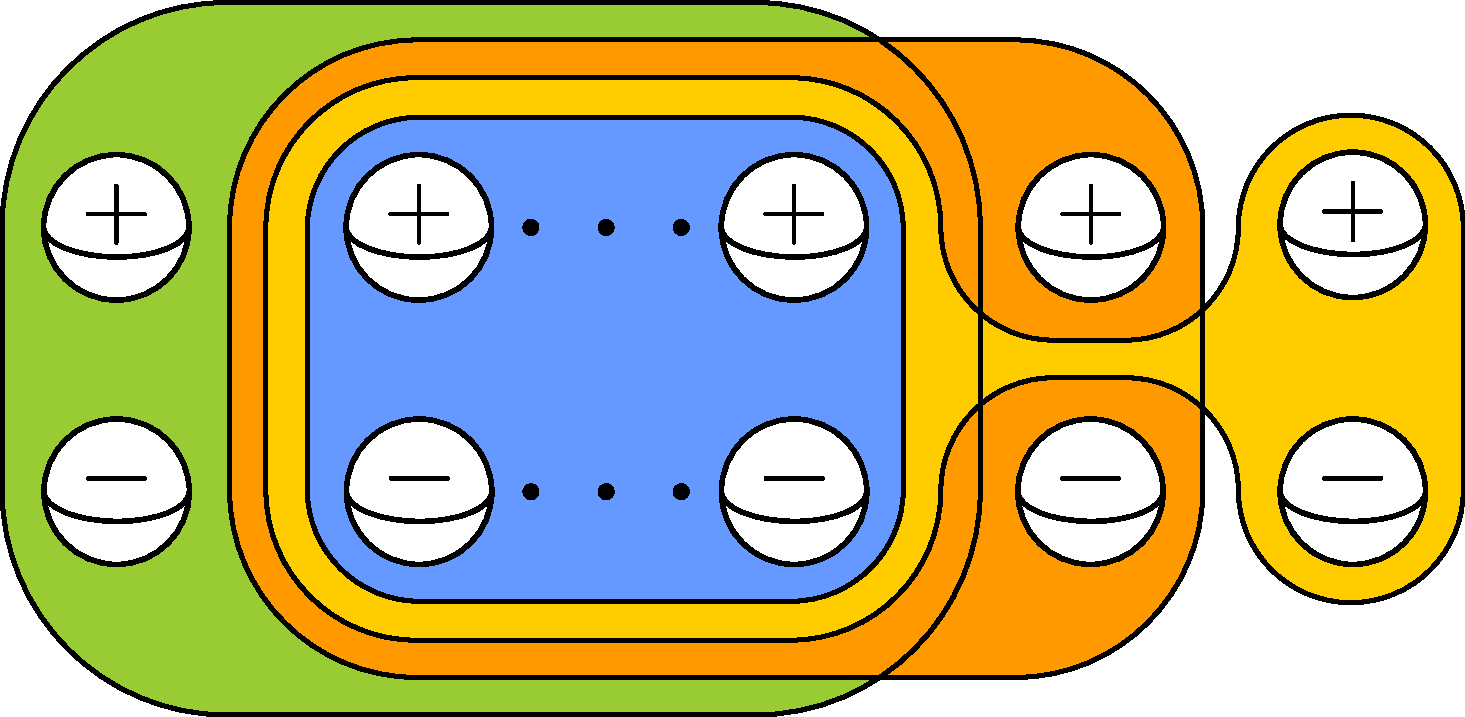
\includegraphics[width=.5\textwidth]{figures/ksharepairgraph0.pdf}
          \caption{
          The sharing pair $v$ is formed by the  green $x_1$ and  orange $x_0$ spheres.
          Transpositions move the sharing pair $v$ either distance 0 in $\mathcal P_x$,
          by swapping orange and green, or
          distance 1, by, for example, swapping orange and yellow.
          Observe that the orange, yellow, and green $M_{k,1}$-bounding spheres form a sharing
          triple for the blue sphere $x$.}
          \label{fig:ksharepair0}
  \end{figure}



  Consider first the action of   transpositions $t$ on
  the sharing pair $v \in \mathcal P_x$.
  If neither $a_0$ nor $a_{n-k}$ are swapped by $t$,
  then the sharing pair $v$ is fixed.
  If both $a_0$ and $a_{n-k}$ are swapped by $t$,
  then $x_0$ and $x_1$ are swapped, so that the sharing pair $v=\{x_0,x_1\}$
  is still fixed.
  If exactly one of $a_0$ or $a_{n-k}$ is swapped by $t$
  transposition then exactly one of $x_0$, $x_1$ are exchanged from the sharing pair,
  so that the transposition action moves the sharing pair $v$ distance 1 in $\mathcal P_x$,
  as shown in Figure \ref{fig:ksharepair0}.


  \begin{figure}[t!]
    \centering
          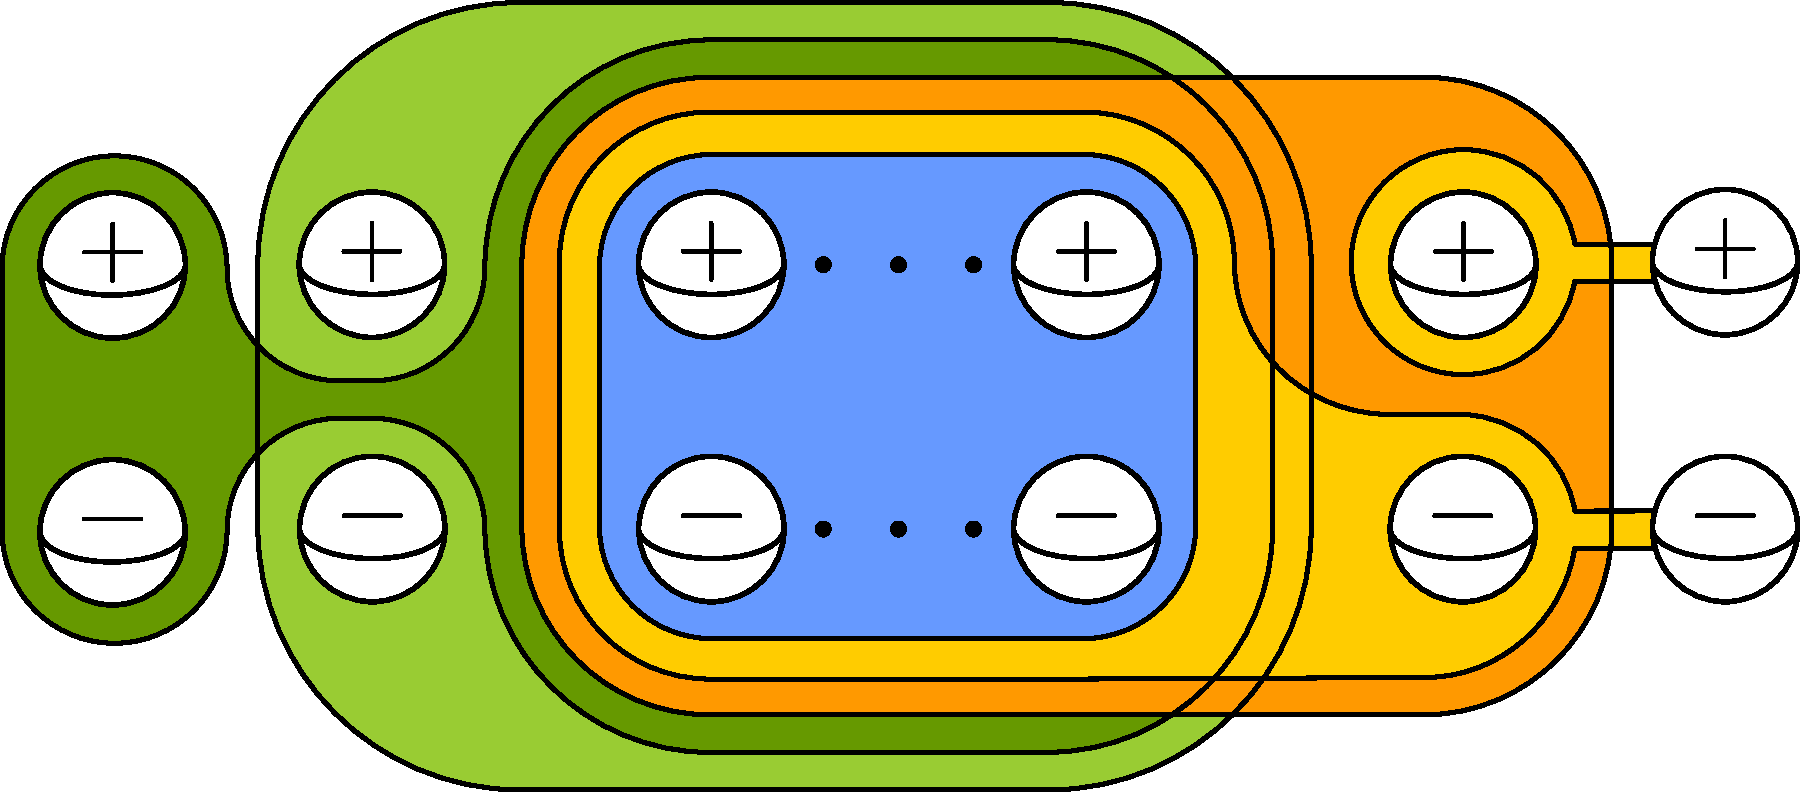
\includegraphics[width=.6\textwidth]{figures/ksharepairgraph1.pdf}
          \caption{The chosen transvection moves $v$
          distance 2 in $\mathcal P_x$.
          Observe that $x_0$ orange, $x_1$ light green,
          $x_2$ dark green, and $t'(x_0)$ yellow can be organized
          into two sharing triples: orange with the greens and yellow with the greens.}
          \label{fig:ksharepair1}
  \end{figure}

  Finally consider the transvection action $t':a_0 \mapsto a_0a_1^{-1}$ on $\mathcal P_x$.
Then $t'(x_0)$ (shown in yellow in Figure \ref{fig:ksharepair1})
intersects $x_0$ (shown in orange) twice and $t'(x_1)=x_1$ (shown in light green).
Since $n-k\geq 4$ there is a nonseparating sphere $a_2$
disjoint and not engulfed from $x_0, x_1, t'(x_0)$.
So there is an $M_{k,1}$ bounding sphere $x_2$ (shown in dark green)
engulfing $a_2$ and such that $\{t'(x_0),x_1,x_2\}$ and $\{x_0,x_1,x_2\}$ are sharing triple---
let $x_2$ be the image of $x_1$ under the transposition $(a_2a_{n-k})$.
Then we have a length 2 path of in $\mathcal P_x$
from $t'(v)$ to $v$:
$$\{t'(x_0),x_1 \} \to \{x_1,x_2\} \to \{x_0,x_1\}.$$
It follows from Putman's Lemma \ref{lemma:putman} that $\mathcal P_x$
is connected.
\end{proof}

We define a map $\aaut  \mathcal S^{sep,k}_n \to \aaut  \mathcal S^{sep,k-1}_n$
as $\phi \mapsto \hat \phi$ by extending $\phi \in \aaut  \mathcal S^{sep,k}_n$
to $M_{k-1,1}$-bounding spheres via $M_{k-1,1}$-sharing pairs.
More explicitly,
if $x \in S^{sep,k-1}_n$
is an $M_{k-1,1}$-bounding sphere
% then by Lemma \ref{lemma:ksharexist}
there is an $M_{k-1,1}$-sharing pair $\{x_0,x_1\}$
that engulfs $x$ uniquely.
Then by Lemma \ref{lemma:sharepreserve},
$\{\phi(x_0),\phi(x_1)\}$
is a sharing pair.
We define $\hat \phi (x)$ as
the $M_{k-1,1}$-bounding sphere
engulfed by $\{\phi(x_0),\phi(x_1)\}$.
By Lemma \ref{lem:kshareconnect}
any other choice $\{x'_0,x'_1\}$
of $x$-sharing pair is connected by
a sequence of sharing triples,
which by Lemma \ref{lemma:sharetrippreserve}
gives a sequence of sharing triples from
$\{\phi(x_0),\phi(x_1)\}$ to $\{\phi(x'_0), \phi(x'_1)\}$,
so that both share the same $M_{k-1,1}$-bounding sphere $\hat \phi(x)$,
which is thus well defined.

Certainly $\hat \phi$ is simplicial.
To see that observe that
if $x$ and $x'$ are disjoint
$M_{k-1,1}$-bounding spheres,
then $n \geq 3k$ so there are disjoint
$M_{k-1,1}$-sharing pairs
that $\phi$ takes to disjoint sharing pairs.
Then $\hat \phi(x)$ is disjoint from $\hat \phi(x')$.
If $y\in \mathcal S^{sep,k}_n$ is disjoint from $x$,
then $y$ is $M_{j,1}$-bounding with $j \leq \frac n 2$
so there is an $x$-sharing pair disjoint from $y$,
with its $\phi$-image disjoint from $\phi(y)$.


\begin{lemma}
  For  $n\geq 3k$ and $k\geq 2$,
  the natural restriction map
   $\aaut  \mathcal S^{sep,k-1}_n \to \aaut  \mathcal S^{sep,k}_n$
   is an isomorphism.
   \label{lemma:highsepinduct}
\end{lemma}

\begin{proof}
 We claim that the constructed map
 extension $ \aaut  \mathcal S^{sep,k}_n \to \aaut  \mathcal S^{sep,k-1}_n $
 given by $\phi \mapsto \hat \phi$
 is the inverse homomorphism to the restriction
 $ \aaut  \mathcal S^{sep,k-1}_n \to \aaut  \mathcal S^{sep,k}_n $
 with
 $\psi \mapsto \psi|_{k}$.
 By definition the restriction of $\hat \phi$ to $\mathcal S^{sep,k}_n $
 is  $\phi$.
 So the extension is injective and restriction is surjective.
 But restriction must also be injective,
 since if $\psi \in \mathcal S^{sep,k-1}_n$
 restricts to the identity,
 then for any $M_{k-1,1}$-bounding sphere $x$
 there is an $x$-sharing pair $\{x_0,x_1\}$ that $\psi$ fixes.
 But then $\psi(x)=x$ is the unique  $M_{k-1,1}$-bounding sphere
 engulfed by $\{x_0,x_1\}$.
\end{proof}


% \thmhighsep*

\begin{proof}[Proof of Theorem  \ref{thm:highsep}]
The proof is by induction on $k$ using Lemma \ref{lemma:highsepinduct}.
Theorem \ref{thm:sep} provides the base case.
\end{proof}


% \section{Coconnected Sphere Systems}
% \label{section:cocspheres}

\section{The Free Factor Complex}
\label{section:ffc}

The free factor complex $\ffn$ is the simplicial complex with a $k$-simplex given by conjugacy classes of length $k+1$ chains of proper free factors.
Bestvina and Bridson announced that the free factor complex is a combinatorial model for $\oout F_n$,
though as of this writing the result remains unpublished \cite{bridson}.


\bridson*


We proceed by proving first that the complex of coconnected spheres of $M_n$
has automorphism group $\oout F_n$.
The complex of coconnected spheres, that was introduced by Hatcher and Vogtmann to prove
homological stability results for $\oout F_n$ in \cite{homstabout},
and the complex of nonseparating spheres \cite{pandit}.
This complex is a fibration over the free factor complex.

\begin{definition}
If $F_n$ can be expressed as the internal free product of subgroups $A,B \leqslant F_n$, then $A$ and $B$ are \emph{free factors} of $F_n$.
The free factor complex has as vertices the conjugacy classes of free factors of $F_n$.
A collection of $A_1, \ldots A_k$ of free factors spans a simplex if there is
are free factors  $A'_1 < \cdots < A'_k$ such that $A_i$ is conjugate to $A'_i$.
We will frequently abuse notation and refer to both a free factor and its conjugacy class as a free factor, as dictated by context.
The distinction is rarely relevant since the free factor complex is known to be flag \cite{MR1660045}.
\end{definition}

Hatcher \cite{MR1660045} characterized the free splitting complex as a complex of spheres in $M_n$.
We define the following three simplicial complexes related to the free factor complex:
\begin{enumerate}[$\cdot$]
\item
Let $\nosep$ be the simplicial complex with $k$-simplices specified by $k+1$ disjoint nonseparating spheres in $M_n$.
\item
Let $\coc n$ be the subcomplex of $\nosep$ with simplices given by collections of spheres that are coconnected (i.e. have connected complement) in $M_n$.
\item
Let $\sfn$ be the barycentric subdivision of the $(n-2)$-skeleton of $\coc n$. Thus vertices of $\sfn$ are coconnected sets of at most $n-1$ spheres, and simplices are given by chains of proper subsets.
\end{enumerate}
For a simplex $\Sigma_0 \subset \cdots \subset \Sigma_k$ of $\sfn$, we obtain a corresponding
simplex of $\ffn$ by the (conjugacy class of) free factors $$\pi_1(M_n-\Sigma_k,x_0) \leqslant \cdots \leqslant \pi_1(M_n-\Sigma_0,x_0)$$ so we obtain a surjection of posets
$$\sfn \to (\ffn)^{op}.$$

A single nonseparating sphere of $M_n$ corresponds to a rank $n-1$ free factor of $F_n$.
The fiber over a rank $k$ free factor corresponds to all choices of collections $n-k$
factors of rank $n-1$ any $j$ of that intersect in a rank $j$ free factor.

We begin by showing

\begin{theorem}
For $n \geq 3$
the natural map
$$ \oout F_n \to \aaut{\sfn} \cong \aaut{\coc n} \cong \aaut{\nosep}$$
is an isomorphism.
\label{thm:twoisos}
\end{theorem}

The result relies on the following theorem of Pandit \cite{pandit}.

\begin{theorem}
 For $n \geq 3$ we have $\aaut{\nosep} \cong \outn$.
\end{theorem}

Our first goal is to show that $\aaut{\sfn} \cong \aaut{\coc n}$.

Let $M_{n,p}$ be the manifold $M_n$ with interiors of $p$ disjoint closed  balls removed. We call $n$ the \emph{genus} of $M_{n,p}$. If $\Sigma$ is a set of disjoint embedded spheres of $M_{n,p}$, we will denote by $M_{n,p}|\Sigma$ the manifold $M_{n,p}$ cut along $\Sigma$.

\begin{lemma}
Automorphisms of $\sfn$ preserve the cardinality of sets of spheres.
\label{lemma:samenumspheres}
\end{lemma}

\begin{proof}
We induct downward on the cardinality of sets of spheres.
We claim as a base case that a set of spheres $\Sigma \in \sfno$ has $n-1$ spheres if and only if
it is adjacent to finitely many sets of spheres in $\sfn$, namely, the proper subsets of $\Sigma$.
If $\Sigma \in \sfno$ has fewer than $n-1$ spheres, then
$M_n|\Sigma$ has genus $k \geq 2$.
The complex of coconnected nonseparating spheres of $M_n|\Sigma$ is isomorphic to $\coc k$, which is infinite.
Choose any nonseparating sphere $a$ of $M_n|\Sigma$. Then $\Sigma \cup \{a\}$ is coconnected in $M_n$ and adjacent to $\Sigma$ in $\sfn$.

Assume that automorphisms of $\sfn$ preserve the size of sets of spheres with at least $k+1$ spheres.
Let $A_k \subset \sfno$ be the sets of spheres of $\sfn$ with $k$ or fewer spheres.
A set of spheres $\Sigma \in A_k$ has $k$ spheres if and only if $\link(\Sigma) \cap A_k$ is finite.
By hypothesis automorphisms of $\sfn$ preserve $A_k$ and its complement, so must preserve the class of sets of $k$ spheres.
\end{proof}

We now prove the first isomorphism of Theorem \ref{thm:twoisos}.\\

\begin{lemma}
For $n\geq 3$ we have $\aaut \sfn \cong \aaut{\coc n}$.
\end{lemma}

\begin{proof}
As $\sfn$ is the barycentric subdivision of the $n-2$ skeleton ${\coc n}^{(n-2)}$, there is a natural map
$$\Phi: \aaut{\coc n} \to \aaut{\sfn}.$$ We will construct the inverse. Let $\phi \in \aaut{\sfn}$.
The vertices of $\sfn$ are the simplices of $\coc n$ with dimension $n-2$ or less.
Then $\phi$ induces a bijection $\phi_\ast$ of simplices of ${\coc n}^{(n-2)}$.
By Lemma \ref{lemma:samenumspheres} we have $\phi_\ast$ preserves the dimension of simplices, so $\phi_\ast$ is an automorphism of ${\coc n}^{(n-2)}$.

It remains to see that $\phi_\ast$ also preserves $n-1$ simplices.
To see this we will show that a collection of $n$ disjoint separating spheres $\Sigma$ form a simplex in $\coc n$ if and only if
$$\coc n \cap  \left ( \bigcap_{x \in \Sigma} \link(x) \right )$$
is finite.
Note that if $\Sigma$ is a coconnected set of $n$ spheres, then $M_n|\Sigma$ is homeomorphic to $M_{0,2n}$. Then $\pi_2(M_n|\Sigma)$ is the free abelian group generated by any $2n-1$ of the balls, and an embedded sphere must be degree at most 1 over any generator.
There are thus finitely many  embedded spheres of $M_n|\Sigma$.
Then $\bigcap_{x \in \Sigma} \link (x)$ contains finitely many vertices of $\coc n$.
Conversely suppose $\Sigma$ is a non-coconnected set of $n$ disjoint spheres.
Then $M_n|\Sigma$ has a component $M'$ with genus at least one and at least two boundary spheres.
Choose a nonseparating sphere $x$ of $M'$, a boundary sphere $y$, and a loop $\alpha$ based at $y$ intersecting $x$ once. The push map of $x$ along $\alpha$ produces a collection $A$ of infinitely many spheres of $M_n$. Each $a \in A$ is nonseparating in $M' \subset M|\Sigma$, so $\{a,x\}$ is coconnected for any $x \in \Sigma$. Then  $A\subset \bigcap_{x \in \Sigma} \link (x)$.
Thus $\phi_\ast$ must also preserve $n-1$ simplices and gives a simplicial automorphism of $\coc n$.
Then $\phi \mapsto \phi_\ast$ gives the inverse homomorphism to $\Phi$.
\end{proof}



Call a collection of $m$ disjoint spheres $\Sigma \subset {\coc n}^{(0)}$ a \emph{bounding $m$-tuple} (pair, triple, etc.) if $\Sigma$ is not coconnected but every proper subset of $\Sigma$ is.
The genus of the bounding tuple is the smaller of the genera of the two components of $M_n|\Sigma$.
The following lemma shows we can detect the genus combinatorially.

\begin{lemma}
The link of a genus $k$ bounding $m$-tuple of $\coc n$ is isomorphic to the join $\coc{k} \ast \coc{n-k-m+1}$.
\label{lemma:itwasseven}
\end{lemma}

\begin{proof}
Consider $\Sigma \subset {\coc n}^{(0)}$ a bounding $m$-tuple with genus $k$.
Then $M_n|\Sigma$ has two components, $R_1 \cong M_{k,m}$ and $R_2 \cong M_{n-k-m+1,m}$.
Let $V_i$ be the complex of coconnected nonseparating spheres in $R_i$.
So $V_1 \cong {\coc {k}}$ and $V_2 \cong \coc {n-k-m+1}$.
We claim that $\link(\Sigma)$ is the join $V_1 \ast V_2$.
Certainly $\link(\Sigma) \subset V_1 \ast V_2$.
Consider sets of spheres $\Sigma_i$ giving simplices of $V_i$.
The $R_i|\Sigma_i$ are connected. $M_n|(\Sigma_1 \cup \Sigma_2)$ is $R_1|\Sigma_1$ and $R_2|\Sigma_2$ glued along $\Sigma$, and hence connected. So $\Sigma_1\cup \Sigma_2$ must be coconnected in $M_n$ and the join $\Sigma_1 \ast \Sigma_2$ lies in $\link(\Sigma)$.
\end{proof}

We now prove the second isomorphism of Theorem \ref{thm:twoisos}.\\

\begin{lemma}
  For $n\geq 3$ we have $\aaut{\coc n} \cong \aaut{\nosep}$.
\end{lemma}

\begin{proof}
Restriction gives a natural map
$$\Phi: \aaut{\nosep} \to \aaut{\coc n}.$$
We will construct the inverse.
Observe that since ${\coc n}^{(0)} = {\nosep}^{(0)}$ any $\phi \in \aaut{\coc n}$ induces a set map $\phi_\ast$ of ${\nosep}^{(0)}$.
If $\phi_\ast$ is a simplicial automorphism, then $\phi \mapsto \phi_\ast$ is the inverse homomorphism to $\Phi$.
As $\nosep$ is a flag complex (Lemma 3 of \cite{souto}), it will suffice to show that $\phi_\ast$ sends pairs of disjoint spheres to pairs of disjoint spheres.
Disjoint nonseparating spheres form a bounding pair if and only if they are not adjacent in $\coc n$.
So it suffices to show that $\phi$ preserves bounding pairs of $\coc n$.
We will demonstrate this through the stronger result that $\phi$ preserves the set of genus $k$ bounding $m$-tuples.

\emph{Case 1.} Suppose $\Sigma$ is a genus $k$ bounding $m$-tuple with $m>2$. Any $\Sigma' \subset {\coc n}^{(0)}$ is a bounding $m$-tuple if and only if $\Sigma'$ does not span a simplex in $\coc n$, but every proper subset of $\Sigma'$ does. Hence if $\phi \in \aaut{\coc n }$, then $\phi(\Sigma)$ is a bounding $m$-tuple.
By Lemma \ref{lemma:itwasseven}, $\link(\Sigma)$ is isomorphic to $\coc {k} \ast \coc{n-k-m+1}$. We can determine $k$ by the maximal simplex dimension on the sides of the join. Then $\phi(\Sigma)$ is also genus $k$.

\begin{figure}[b!]
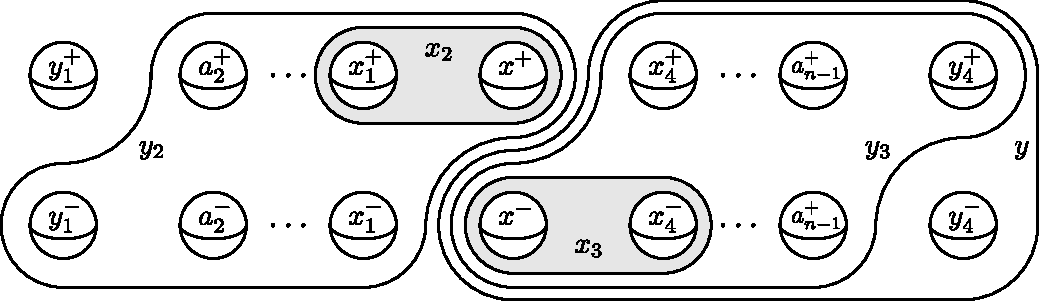
\includegraphics[width=\textwidth]{figures/spheresagain.pdf}
\caption{
The manifold $M_n|\{a_i\}_{i=1}^n$ is a 3-sphere with $2n$ balls removed.
We obtain $M_n$ by again identifying the spheres with $+$ and $-$ labels via a vertical reflection.
The spheres $\Sigma'=\{x_i,y_i\}_{i=1}^4$ are such that $M_n|\Sigma'$ contains $x$ and $y$ in disjoint copies of $M_{0,4}$. The $M_{0,4}$ containing $x$ (identify $x^+$ and $x^-$) is shaded. The $M_{0,4}$ containing $y$ is the exterior of $y_2$ and $y_3$.
}
\label{fig:spherediagram}
\end{figure}

\medskip \noindent \emph{Case 2.} Suppose $\Sigma=\{x,y\}$ has $m=2$ spheres.
Choose a collection $\Sigma'$ of disjoint nonseparating spheres such that  there are two separate components of $M_n|\Sigma'$ homeomorphic to $M_{0,4}$ and containing $x$ and $y$ respectively.
We can construct $\Sigma'$ as follows.
$M_n|\Sigma$ has two components, homeomorphic to $M_{k,2}$ and $M_{n-k-1,2}$.
So we have a set of spheres $\{a_i\}_{i=1}^n$ coconnected in $M_n$ disjoint from $y$ with $a_{k+1}=x$.
Choose $x_2,x_3,y_2,y_3$ as shown in figure \ref{fig:spherediagram} and relabel $a_1=y_1$, $x_{1}=a_k$, $x_4=a_{k+2}$, $y_4=a_n$.
Then
$\{x_1,\ldots, x_4\}$ (resp. $\{y_1, \ldots, y_4\}$ are the boundary spheres of a component of $M|\Sigma'$ homeomorphic to $M_{0,4}$ and containing $x$ (resp. $y$).
Further $\{x,x_1,x_2\}$ and $\{x,x_3,x_4\}$ are genus 0 bounding triples. Let $\Sigma' =\{x_i,y_i\}_{i=1}^4$.



By Case 1 we have that $\{\phi(x_1), \ldots, \phi(x_4)\}$ is a genus 0 bounding $4$-tuple and $\{\phi(x),\phi(x_1),\phi(x_2)\}$ and $\{\phi(x),\phi(x_3),\phi(x_4)\}$ are genus 0 bounding triples.
So $\{\phi(x_1), \ldots, \phi(x_4)\}$ define a component of $M|\Sigma'$ homeomorphic to $M_{0,4}$ and containing $\phi(x)$.

If $\{x_1, \ldots, x_4\} \neq \{y_1, \ldots, y_4\}$ then
 $\phi(x)$ and $\phi(y)$ lie in disjoint $M_{0,4}$ homeomorphic components of $M|\phi(\Sigma')$.
Then  $\phi(x)$ and $\phi(y)$ are are disjoint. They are also not adjacent in $\coc n$, so they are bounding a pair.

Suppose $\{x_1, \ldots, x_4\} = \{y_1, \ldots, y_4\}$.
Then $n=3$ and $M_3|\{x_i\}_{i=1}^4$ is homeomorphic to two copies of $M_{0,4}$.
As $x,y$ form a bounding pair, the bounding triples must be
$\{x,x_1,x_2\}$, $\{x,x_3,x_4\}$, $\{y,x_1,x_2\}$, and $\{y,x_3,x_4\}$.
Then the $\phi$ image of these triples are
bounding triples giving $\phi(x)$ and $\phi(y)$ contained in disjoint $M_{0,4}$.
Then $\phi(x)$ and $\phi(y)$ are disjoint and must form a bounding pair.
\end{proof}


% \section{Complex of Surfaces}
%
% \noindent \emph{Def}
% A genus $g$ \emph{rosebud} is the wedge of a sphere and a genus $g$ rose.
% We consider spheres genus 0 rosebuds, and roses degenerate rosebuds.\\
% \\
%
% \noindent \emph{Claim}
% Every embedded compact
% closed orientable surface in $M_g$
% is homotopy equivalent to a sphere, rose, or rosebud.\\
% \\
% \emph{Proof.}
% Consider the image in $p^3$ minus spheres.
% Every disk is compressible.\qed\\
% \\
%
% \noindent \emph{Claim}
% An embedded surface $p_g$ has $\pi_1(S_g)$ contains a
% free factor at most rank $g$.\\
% \\
% \emph{Proof.}
% If $\pi_1(S \hookrightarrow M)$ contains a free factor rank $k$,
% then $p$ intersects at least $k$ disjoint spheres
% in $M$. Then there are at least $k$
% compressible disks with $\partial D \subset S$.
% Each one kills a generator of $\pi_1(S)$
% \\
%
% \noindent \emph{Claim}
% There is a correspondence between
% homotopy classes of embedded rosebuds
% in $M_n$ and one edge Bass Serre graph-of-groups
% decompositions of $F_n$.\\
% \\
% \emph{Proof.}
% By Van Kampen every rosebud gives a graph of groups.
% Conversely if $F_n =  \pi_1 ( A \leftrightarrow C \rightarrow B )$
% then there is a basis $\{a_i\}_{i \in n}$ of $F_n$
% with the first $k$ in $A$ and the last $n-k$ in B.
% This corresponds to a system of nonseparating spheres.
% There is a unique separating sphere $p$ which separates the $A$
% spheres from the $B$ spheres.
% From a basepoint on $p$ there is a rose whose petals give the arcs forming
% a basis of $C$. \qed\\
% \\
%
% \noindent \emph{Def. }
% The graph of embedded rosebuds
% $\mathcal R_n$
% has embeddings of rosebuds (and roses) of genus at most $n$ as vertices.
% Two embedded rosebuds are adjacent if the embeddings of their
% homotopy classes differ by
% the wedge of a (homologically nontrivial?) 1- or 2-sphere.\\
%
%
% 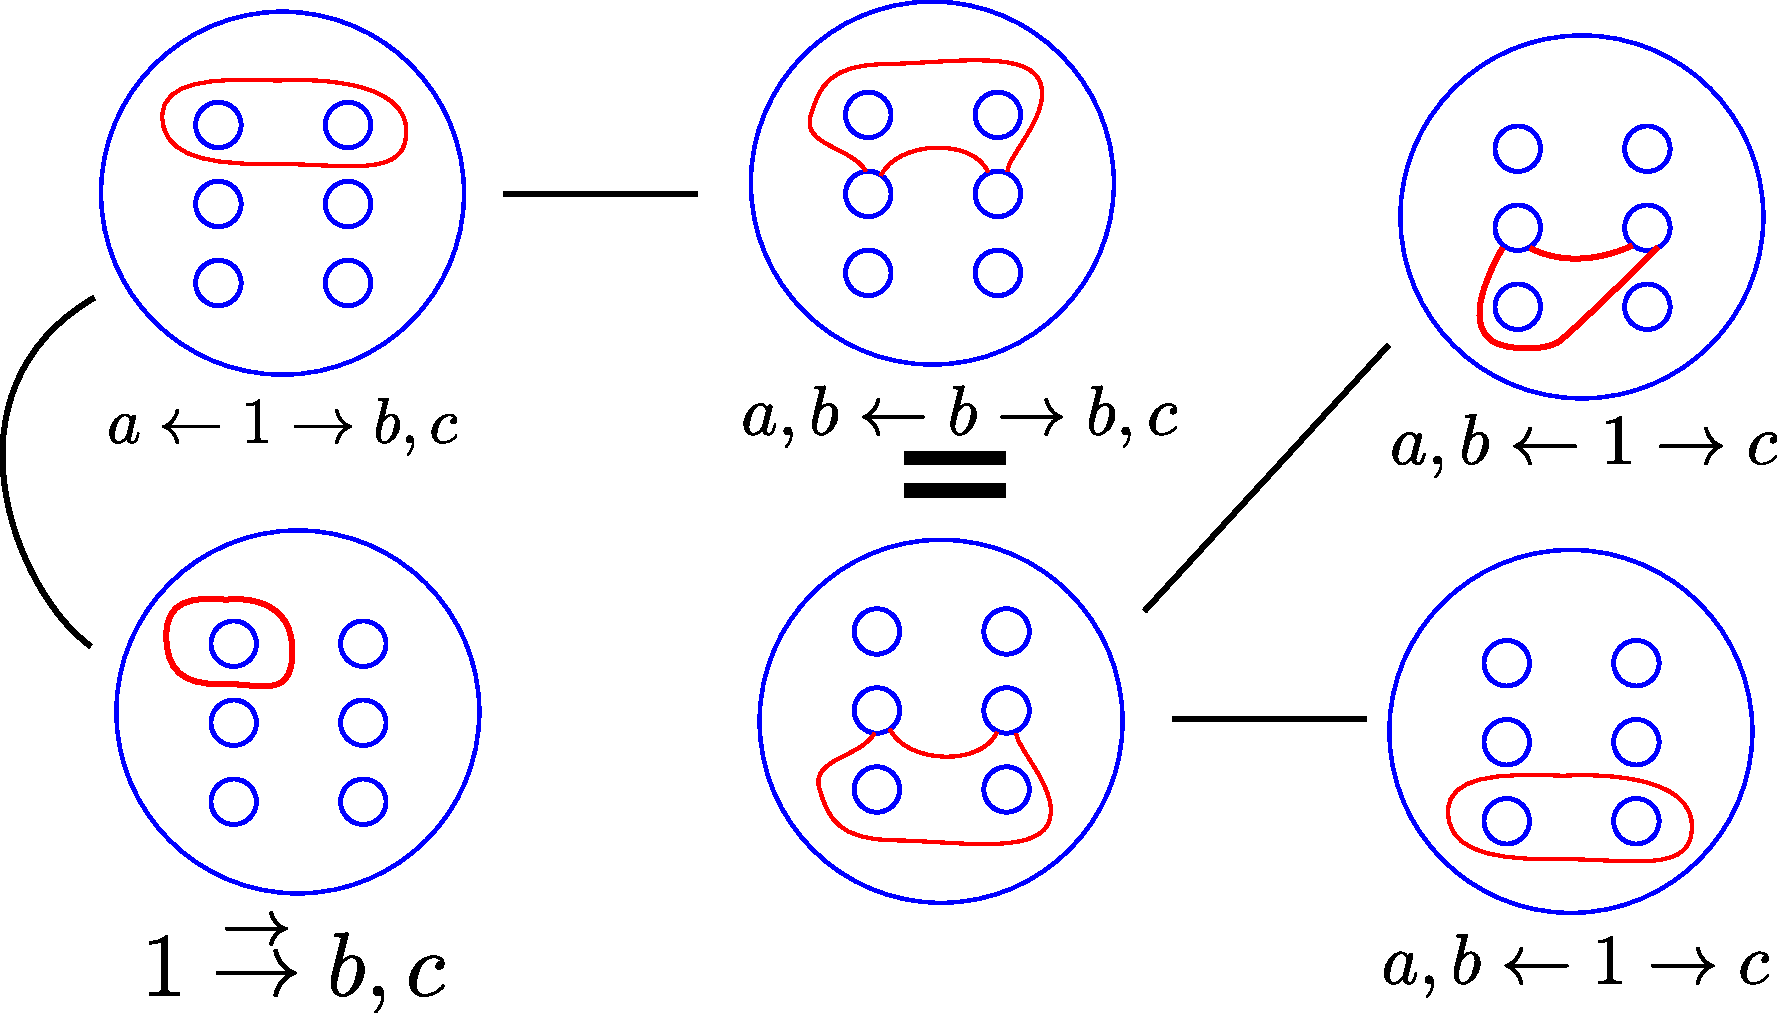
\includegraphics[width=.8\textwidth]{figures/rosebudgraph.pdf}
%
%
% $\mathcal R_n$ is equivalent to the graph of one-edge Bass Serre
% graph-of-group decompositions of $F_n$ with adjacency given by
% the following moves:
% \begin{enumerate}
%   \item tube tunneling at $a \in A - B$
%   $$A \leftarrow C \rightarrow B  \ \Leftrightarrow  \ A \leftarrow C \ast a \rightarrow B \ast a$$
%   \item nonseparating sphere scooping (primitive $b \not \in A$)
%   $$
%    C \stackrel{\rightarrow}{\rightarrow} A \ast A'b
%     \ \Leftrightarrow  \
%     C \stackrel{\rightarrow}{\rightarrow}  A \ast A'
%      \ \Leftrightarrow  \
%   b \ast C \leftarrow C \rightarrow  A \ast A'
%   $$
% \end{enumerate}



Dyer and Formanek gave an algebraic proof
of the fact that automorphisms of automorphisms of free groups are simply automorphisms of free groups \cite{doi:10.1112/jlms/s2-11.2.181}.
Vogtmann and Bridson gave a more recent geometric proof \cite{MR1769698}.
\begin{theorem}
  The natural maps
  $$\aaut F_n \to \aaut \aaut F_n$$
  and
  $$\oout F_n \to \aaut \oout F_n$$
  are isomorphisms for $n \geq 3$.
  In particular $\oout \oout F_n =1$ and the center of $\oout F_n$ is trivial.
  \label{theorem:outout}
\end{theorem}


\begin{lemma} Automorphisms of the free factor complex preserve the rank of free factors.

  Let $\phi \in \aaut \ffn$ and let $A$ be a free factor of $F_n$.
  Then $A$ and $\phi(A)$ have the same rank.
  \label{lemma:ffsize}
\end{lemma}

\begin{proof}
  Suppose that $A$ is a free factor of $\ffn$.
  Then the link of $A$ is a join
  $$
  \link A \cong  \mbox{span} \{B \in \ffn^{(0)} \ | \ B < A\} \ast \mbox{span} \{B \in \ffn^{(0)}  \ | \ A<B\}
  $$
  between the sub- and  super-factors of $A$.
  So if $A$ is rank $k$ then
  $\{B \in \ffn^{(0)} \ | \ B < A\}$ spans a dimension $k-2$ subcomplex
  isomorphic to $\mathcal{FF}_k$ and similarly $\{B \in \ffn^{(0)}  \ | \ A<B\}$
  spans a dimension $n-k-2$ subcomplex
  isomorphic to $\mathcal{FF}_{n-k}$.
  If $\phi \in \aaut \ffn$ then $\phi$ preserves this join and $\phi(A)$ must be either rank $k$ or $n-k$.

  Let $\mathcal G$ be the subcomplex of $\ffn$ spanned by rank 1 and rank $n-1$ free factors.
  Then $\mathcal G$ is a connected and bipartite with the rank 1 and rank $n-1$ factors forming the parts of the bipartition.
  Then if $A,A' \in \mathcal G^{(0)}$ are free factors the same rank, the free factors $\phi(A),\phi(A')$ must have the same rank for any $\phi \in \aaut \ffn$.
  Assume to the contrary that there is $\phi \in \aaut \ffn$ an automorphism
  and a rank $n-1$ free factor $A$ with $\phi(A)$ rank 1.
  Then $\phi$ must swap the bipartition of $\mathcal G$.
  In fact, there is a map $\aaut \ffn \to \Z/2$ taken by sending $\phi' \in \aaut \ffn$ to the generator of $\Z/2$
  if $\phi'$ swaps the bipartition on $\mathcal G$.
  Then if $G = \langle \phi, \oout F_n \rangle  \leq \aaut \ffn$ is the subgroup generated by $\oout F_n$ and the automorphism $\phi$
  we have an exact sequence
  $$
  \begin{tikzcd}
    1 \arrow{r} &
    \oout F_n \arrow{r} &
    G  \arrow{r}&
    \Z/2  \arrow{r}&
    1
  \end{tikzcd}
  $$
  But by Theorem \ref{theorem:outout} we know $\oout F_n$ is centerless and $\oout \oout F_n = 1$,
  so we may apply Lemma
  \ref{centerout}
  to conclude that $G \cong \oout F_n  \times \Z/2$.
  Then there is an order two automorphism $t$ of $\ffn$ that swaps the bipartition of $\mathcal G$
  and commutes with $\oout F_n$.
  Then there is rank one free factor $\langle b \rangle$ and free factor $A$ with rank $n-1$
  such that $t(\langle b \rangle )=A$.
  Let $A$ have free basis $a_1,\ldots,a_{n-1}$ with $b=a_{n-2}$ if $b \in A$.
  Then the transvection $\phi''$ with $b \mapsto ba_1$ and $a_i \mapsto a_i$
  is an outer automorphism acting on the free factors with
  $$
  A = \phi''(A) =\phi'' t(\langle b \rangle ) = t \phi'' ( \langle b \rangle ) = t ( \langle ba_1 \rangle  )
  $$
  but this contradicts that $t$ is injective.
  It must be that for any automorphism $\phi \in \ffn$
  the rank of $A$ and $\phi(A)$ are the same if $A$ is rank 1 or rank $n-1$.

  But then if $A$ is a rank $k$ free factor, the link of $A$ is a join with sides of dimension $k-2$ and $n-k-2$,
  and any rank $n-1$ free factor $B$ containing $A$ is on the dimension  $n-k-2$ side.
  So the link of $\phi(A)$  is isomorphic to $\mathcal{FF}_k \ast \mathcal{FF}_{n-k}$
  with $\phi(B)$ the rank $n-1$ free factor on the dimension $n-k-2$ side.
  But then $\phi(A)$ must be rank $k$ as well.
\end{proof}


% \begin{theorem}
%   The natural map
%   $$
%   \oout F_n \to \mathcal{FF}_n
%   $$
%   is an ismorphism for $n \geq 3$.
%   \label{}
% \end{theorem}

\bridson*

\begin{proof}
  Let $A$ be a free factor of rank $n-1$.
  Recall the bijection between the conjugacy classes of rank $n-1$ free factors and homotopy classes of nonseparating spheres of $M_n$.
  There is a unique nonseparating sphere $z$ in $M_n$
  specifying the conjugacy class of a free factor $A_x$ in $\pi_1 (M_n-x,q)$.
  So if $\phi \in \aaut \ffn$ we define a map of spheres by defining $\hat \phi(x)$ to be the sphere
  specifying the free factor $\phi(A_x)$ for any nonseparating sphere $x$.
  If $\Sigma$ is a coconnected set of $k$ spheres
  then we have the conjugacy class representatives of free factors $A_x$ for $x\in \Sigma$ such that $\bigcap_{x \in \Sigma'} A_{x'}$
  is a free factor of rank $n-|\Sigma'|$ for any $\Sigma' \subset \Sigma$.
  Coversely, if $A_1, \ldots, A_\ell$ are rank $n-1$ free factors bijecting to nonseparating spheres $x_1, \ldots, x_\ell$
  such that $\bigcap_{j \in s} A_j$ a rank $n-|s|$ free factor for any $s \subset \{1, \ldots, \ell\}$ then it must be that
  $$F_n  = \bigcap_{j=1}^\ell A_j \ast \langle a_1 \rangle  \ast \cdots \ast \langle a_\ell \rangle$$
  for some $a_j \in A_j$ so that $\{x_j\}_{j=1}^\ell$ must be coconnected nonseparating spheres.

  Then by Lemma \ref{lemma:ffsize} this property is preserved by $\phi$, so that
  we have a well defined simplicial map $\hat \phi: \sfn \to \sfn$
  with
  $\hat \phi (\Sigma) = \{ \hat \phi(x) \ | \ x \in \Sigma \}$.
  This gives us homomorphisms
  $$
  \begin{tikzcd}
    \oout F_n \arrow[hookrightarrow]{r} &
    \aaut \ffn \arrow{r}{\hat{\cdot}} &
    \aaut \sfn\\
    &
    \phi \arrow[mapsto]{r} & \hat \phi
  \end{tikzcd}
  $$
If $\hat \phi$ fixes every coconnected set of sphere then $\phi$ must fix every free factor,
so these homomorphisms are in fact isomorphisms.
\end{proof}


% !TEX root = thesis.tex
\chapter{Complex of Strongly Separating Curves}
\label{chap:strongsep}

The content of this chapter is joint work with Alan McLeay at the University of Glasgow.

The complex of strongly separating spheres $\mathcal C^{ss}S_{g,p} \subset \mathcal C S_{g,p}$ is the induced subcomplex
whose vertices are
separating curves in the genus $g$, $n$-punctured surface $S_{g,p}$
such that both components have complexity $3g'+p'-3 > 0$.
In particular
$$
\css S_{g,p} = \csep S_{g,p}
$$
is the complex of separatng curves whenever $p \leq 1$,
and otherwise $
\css S_{g,p} \subset \csep S_{g,p}
$
is the subcomplex discarding curves bounding pairs of pants.

In
\cite{MR3724237,MR3620458}
Bowditch demonstrates that if $\aaut \css S_{g,p}$ is the mapping class group,
then
 every quasi-isometry of the
Weil-Petersson metric on Teichm\"uller space associated to $S_{g,p}$
is induced by a mapping class of $S_{g,p}$.
In \cite{bowditch} Bowditch completes the reduction by showing that
$\aaut \css S_{g,p}$ is the mapping class group in all but finitely many cases.


\begin{theorem}
  \label{thm:bowditch}
 If $g+p\geq 7$, then
 the natural map
 $$\mcg^\pm \left ( S_{g,p} \right ) \to \aaut \left ( C^{ss}(S_{g,p}) \right )$$
 is an isomorphism.
\end{theorem}

Bowditch asks which of the remaining low complexity $g+p \leq 6$ cases have $\aaut \css S_{g,p}$ given by the mapping class group.
In this chapter we provide an independent proof of Bowditch's result that settles some of these low complexity cases and
 provide evidence that the remaining unknown cases of $\aaut \css$ are themselves mapping class groups.
The goal of this chapter is to prove the following theorem.

\begin{theorem}
  \label{thm:css}
The natural map
 $$\mcg^\pm \left ( S_{g,p} \right ) \to \aaut \left ( C^{ss}(S_{g,p}) \right )$$
 is an isomorphism for the green entries in the table below.
\end{theorem}

\begin{tabular}{ | c | c| c| c| c| c| c|c| }
  \hline
  $g$ $\backslash$ $p$ & 0 & 1 & 2 & 3 & 4 & 5 & 6  \\
  \hline
  0 & {\color{red}$\times$} & {\color{red}$\times$} & {\color{red}$\times$} & {\color{red}$\times$} & {\color{red}$\times$} & {\color{red}$\times$} & {\color{red}$\times$} \\
  \hline
  1 & {\color{red}$\times$} & {\color{red}$\times$} & {\color{red}$\times$} & {\color{red}$\times$} & ? & ?  & \cite{bowditch} \\
  \hline
  2 & {\color{red}$\times$} & {\color{red}$\times$} & {\color{red}$\times$} &  ? & {\color{green}$\checkmark$} & \cite{bowditch}  & \cite{bowditch} \\
  \hline
  3 & \cite{commensurations} &\cite{kida} & {\color{green}$\checkmark$} & {\color{green}$\checkmark$} &\cite{bowditch}& \cite{bowditch}&\cite{bowditch} \\
  \hline
  4 & \cite{commensurations} &\cite{kida}& {\color{green}$\checkmark$}  & \cite{bowditch}&\cite{bowditch}&\cite{bowditch}&\cite{bowditch} \\
  \hline
  5 & \cite{commensurations} &\cite{kida}&\cite{bowditch}&\cite{bowditch}&\cite{bowditch}&\cite{bowditch}&\cite{bowditch} \\
  \hline
  6 & \cite{commensurations} &\cite{kida}& \cite{bowditch} & \cite{bowditch}& \cite{bowditch}& \cite{bowditch} & \cite{bowditch} \\
  \hline
\end{tabular}

We also show that in the unsettled cases of $\css S_{1,4}$, $\css S_{1,5}$, and $\css S_{2,3}$,
any automorphisms with respect the fibers of the point-forgetting projection arise from mapping class groups,
and that if $\css S_{1,4}$ is a mapping class combinatorial model, so is $\css S_{2,3}$.

\section{Point-Forgetting Projection}
\label{sect:strongpoint}

Notice that to have any edges at all in the graph $\css S_{g,p}$ it must be that $$3g+p \geq 7.$$
As we have seen in Chapter \ref{chap:birman}, the puncture forgetting map
$$
\begin{tikzcd}
\css S_{g,p} \arrow[r, twoheadrightarrow] & \csep S_g
\end{tikzcd}
$$
is a simplicial quotient map for $p \leq 2$.
In particular $\css S_{2,1}$ and $\css S_{2,2}$
have quotients onto $\csep S_{2}$, which is disconnected.
All of these disconnected complexes have automorphisms permuting
the connected components, so that their automorphism groups contain an infinite symmetric group.
We conjecture that the strongly separating curve complex $\css S_{g,p}$
is rigid whenever it
 is connected.

\begin{lemma}
  \label{thm:cssgraphs}
  Automorphisms of the strongly separating curve complex induce isomorphisms on region adjacency graphs.

  Let $\phi \in \aaut \css S_{g,p}$ and let $\Delta$ be any simplex of $\css S_{g,p}$.
  Then $\phi$ induces an isomorphism  between the region adjacency graphs
  $\mathcal G_\Delta$ and $\mathcal G_{\phi(\Delta)}$.
\end{lemma}

\begin{proof}
  The proof of \ref{lemma:adjgraph} shows in particular that $\phi$ induces
  an incidence preserving bijection between the edges of $\mathcal G_\Delta$ and $\mathcal G_{\phi(\Delta)}$.
  But since every sphere of $\css S_{g,p}$ is separating,
  every simplex $k-1$ simplex $\Delta$ gives an adjacency graph $\mathcal G_\Delta$
  that is a tree with $k$ edges and $k+1$ vertices.
  But then by Whitney's Theorem \ref{thm:whitney}
  an incidence preserving bijection between $\mathcal G_\Delta$ and $\mathcal G_{\phi(\Delta)}$
  must be an isomorphism.
\end{proof}

\begin{definition}
  We call a region adjacency graph \emph{linear} if it is a tree with exactly 2 leaves.
  Recall that a leaf is a degree 1 vertex of a tree.
\end{definition}


\begin{lemma}
  \label{thm:csstype}
  Automorphisms of the strongly separating curve complex preserve the topological type of curves.

  Let $\phi \in \aaut \css S_{g,p}$ and supposed that $\aaut \css S_{g,p}$ is connected.
  Then for any curve $x$ in $\css S_{g,p}$ there is a homoemorophism $\psi$ of $S_{g,p}$
  such that $\psi(x)=\phi(x)$.
\end{lemma}

\begin{proof}
  We will consider adjacency graphs and consider several cases depending on the genus of the surface.
  In each case we will utilize a combinatorial characterization of the curve in terms of the region adjacency graph
  of a maximal simplex and apply Lemma \ref{thm:cssgraphs}.
  % \begin{enumerate}[{Case} 1.]

  \begin{figure}[h!]
    \centering
    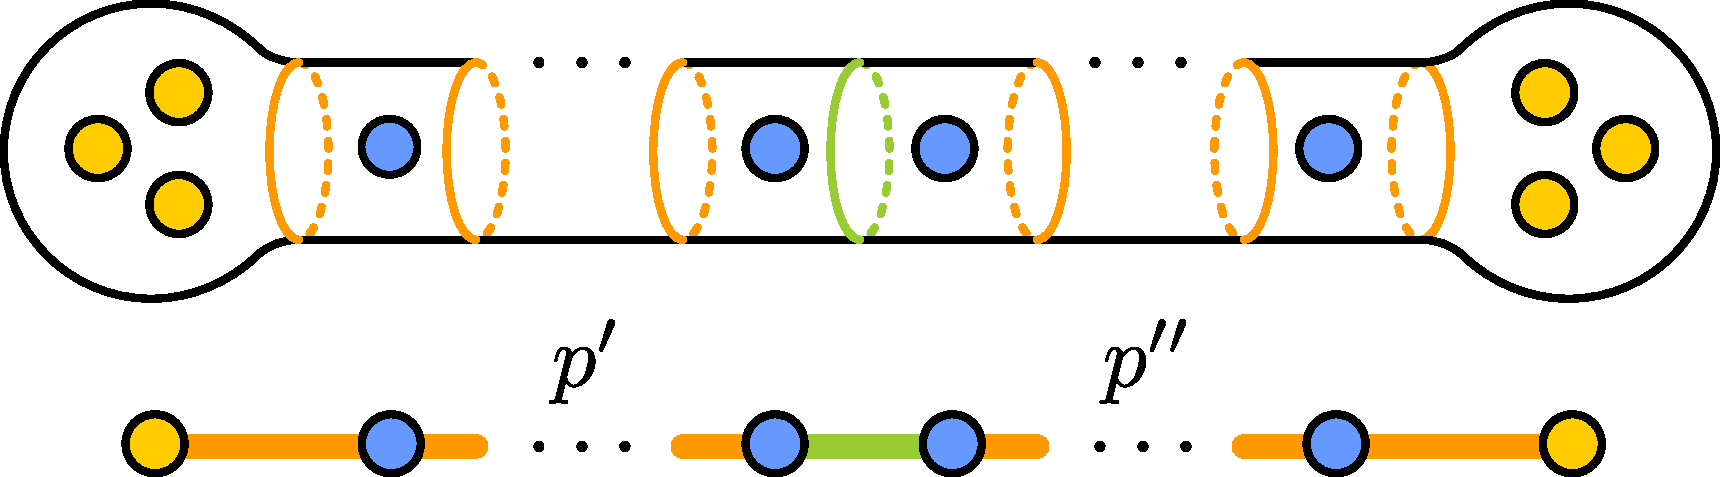
\includegraphics[width=.6\textwidth]{figures/cssmaxsimp4.pdf}
    \caption{A maximal simplex and the region adjacency graph.}
    \label{fig:cssmaxsimp4}
  \end{figure}

    \emph{Case 1.} Suppose that $g=0$.

    Let $x$ be a separating curve of $S_{0,p}$.
    As in Figure \ref{fig:cssmaxsimp4} we may choose a maximal simplex $\Delta$ of $\css S_{g,p}$
    containing $x$ so that the region adjacency graph $\mathcal G_\Delta$ is linear.
    Then the curve $x$ bounds an $S_{0,p'}$ if and only if the edge $e_x$ is distance $p'-3$ from a leaf of $\mathcal G_\Delta$.
    The result then follows from Lemma \ref{thm:cssgraphs}.

    \begin{figure}[h!]
      \centering
      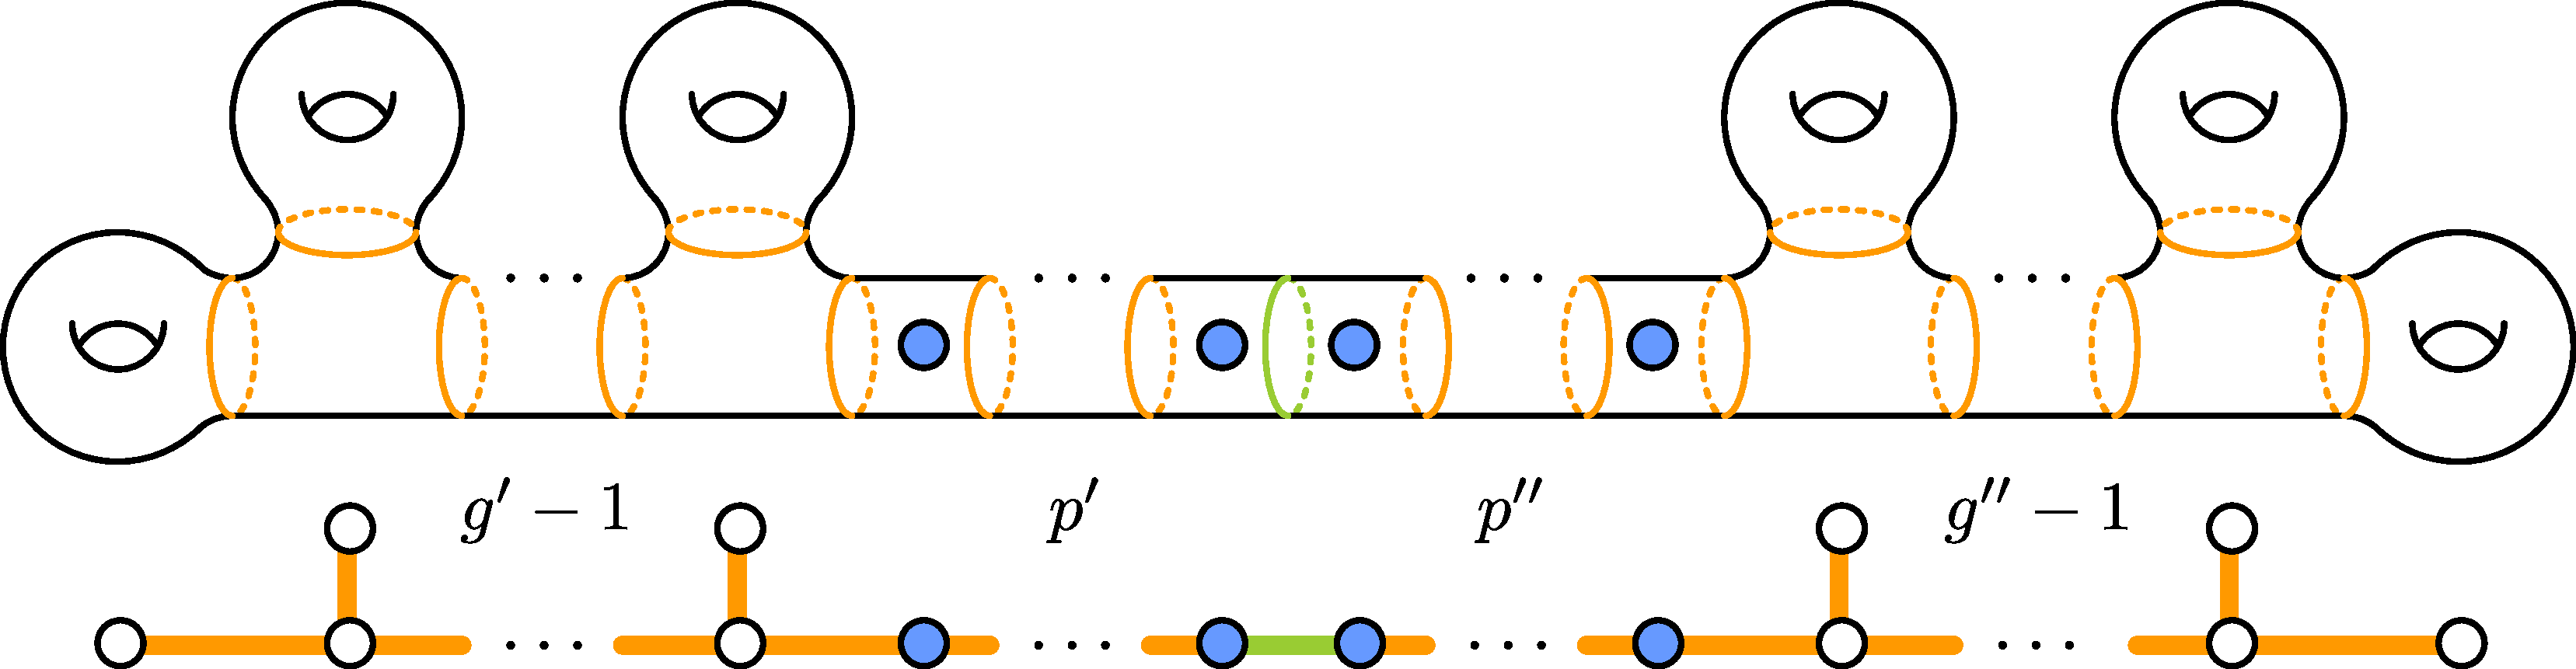
\includegraphics[width=\textwidth]{figures/cssmaxsimp1.pdf}
      \caption{A maximal simplex and the region adjacency graph.}
      \label{fig:cssmaxsimp1}
    \end{figure}
    \emph{Case 2.} Suppose that $g\geq 2$.

    Suppose that $x$ is a separating curve with sides $S_{g',p'}$ and $S_{g'',p''}$ with both $g',g''>0$.
    As in Figure \ref{fig:cssmaxsimp1} we may choose a maximal simplex $\Delta$ of $\css S_{g,p}$ containing $x$ that has no
    curves bounding a 3-punctured disk.
    Note that the adjacency graph $\mathcal G_\Delta$ of a maximal simplex $\Delta$ is a tree with vertices at most degree 3.
    Then $\Delta$ has a curve bounding a 3-punctured disk if and only if
    with the tree $\mathcal G_\Delta$ has exactly $g$ leaves and $g+p-2$ non-leaves.
    Then $e_x$ is a cut edge of the tree $\mathcal G_\Delta$ separating $\mathcal G_\Delta$ into two trees with
    with $g'$  and $g''$  leaves, respectively, and $g'+p'-2$  and $g''+p''-2$ non-leaves, respectively.
    Then by Lemma \ref{thm:cssgraphs} $\phi(x)$ is such a cut edge in the isomorphic tree $\mathcal G_{\phi(\Delta)}$
    so that the sides of $\phi(x)$ must be an $S_{g',p'}$ and an $S_{g'',p''}$.

    \begin{figure}[h!]
      \centering
      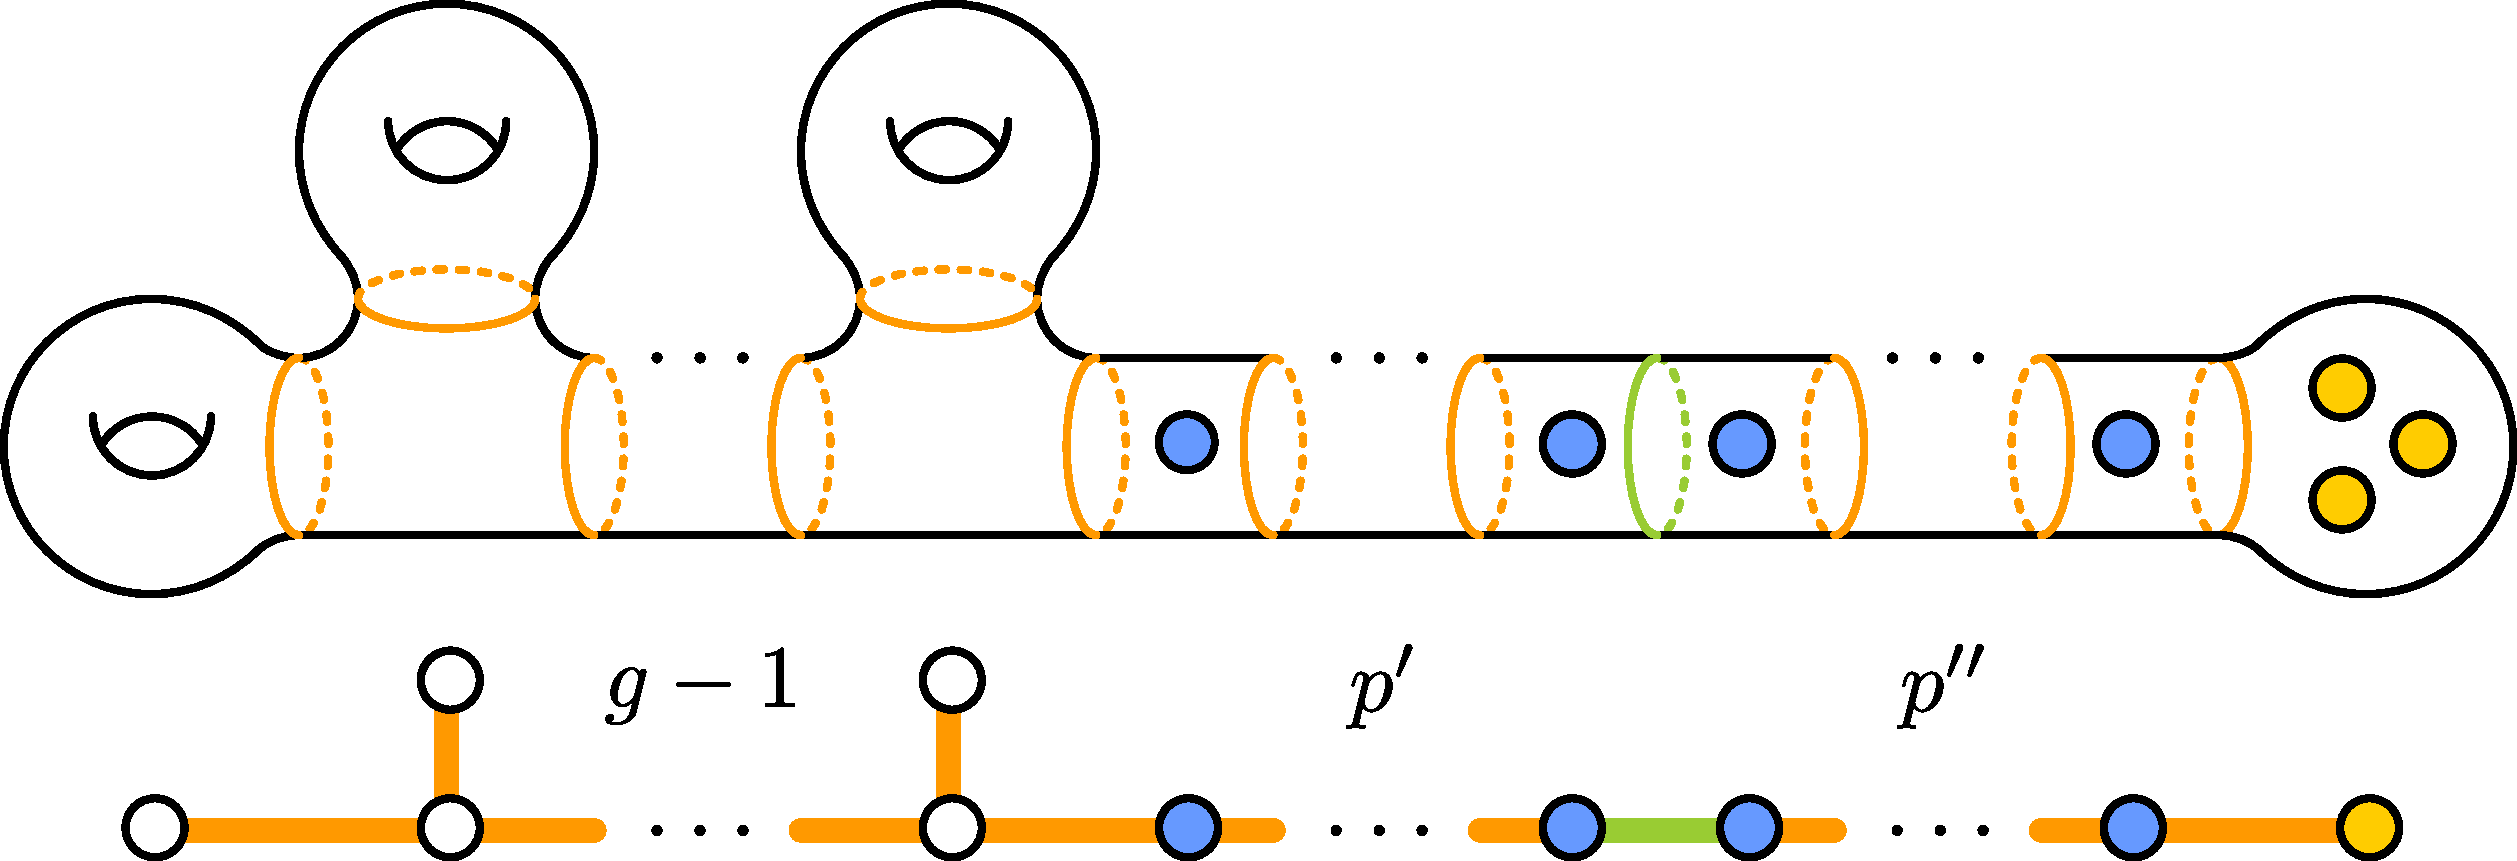
\includegraphics[width=.8\textwidth]{figures/cssmaxsimp2.pdf}
      \caption{A maximal simplex and the region adjacency graph.}
      \label{fig:cssmaxsimp2}
    \end{figure}

    If instead $x$ has an $S_{0,p'}$ side,
    then any maximal simplex $\Delta$ containing $x$ has a region adjacency graph $\mathcal G_\Delta$
    with greater that $g$ leaves.
    We may choose a simplex $\Delta$ as in Figure \ref{fig:cssmaxsimp2} containing $x$ and with a a region adjacency graph $\mathcal G_\Delta$
    that has $g+1$ leaves and $x$ separates one leaf $v$ representing a 3-punctured disk from the other leaves,
    and the component of the leaf $v$ in the cut tree $\mathcal G_\Delta - e_x$ has $p'-3$ edges.
    Then by Lemma \ref{thm:cssgraphs} $\phi(x)$ is such a cut edge in the isomorphic tree $\mathcal G_{\phi(\Delta)}$, and
    by the previous subcase the  $g$ leaves $\phi_\ast(w)$ of $\mathcal G_{\phi(\Delta)}$ for $w\neq v$
    represent curves bounding $S_{1,1}$s so that $\phi(v)$ must represent a 3-punctured disk and its component in
    the cut tree $\mathcal G_{\phi(\Delta)} - e_{\phi(x)}$ specifies an $S_{0,p'}$ bounded by $\phi(x)$.

    \emph{Case 4.}  Suppose that $g=1$.

    \begin{figure}[h!]
      \centering
      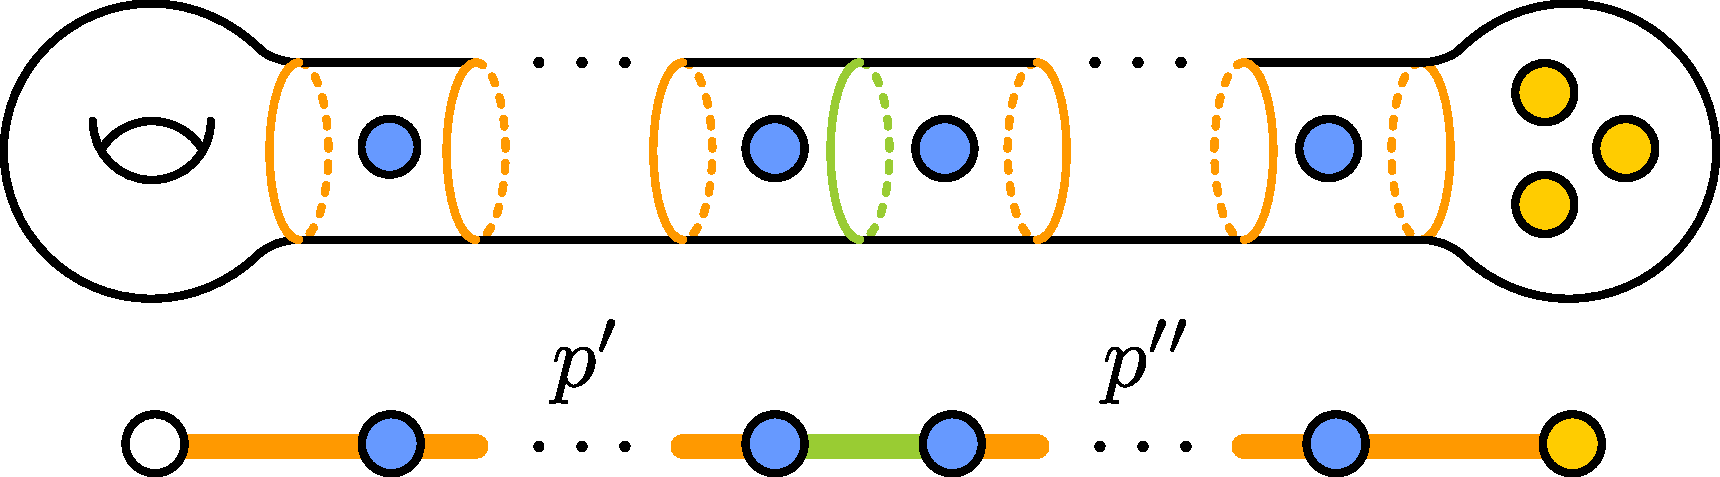
\includegraphics[width=.6\textwidth]{figures/cssmaxsimp3.pdf}
      \caption{A maximal simplex and the region adjacency graph.}
      \label{fig:cssmaxsimp3}
    \end{figure}

    Let $x$ be a strongly separating curve of $S_{1,p}$.
    As in Figure \ref{fig:cssmaxsimp3} we may choose a maximal simplex $\Delta$ of $\css S_{g,p}$
    containing $x$ so that the region adjacency graph $\mathcal G_\Delta$ is linear.
    Then by Lemma \ref{thm:cssgraphs} we have that $\phi$ induces an automorphism of $\mathcal G_\Delta$.
    Let $x_0$ and $x_1$ be the curves of $\Delta$ with $x_0$ bounding the $S_{1,1}$ and
    $x_1$ bounding the 3-punctured disk. We can be sure that $\phi(x_0)$ and $\phi(x_1)$ each
    bound either a 3-punctured disk or an $S_{1,1}$, since a leaf of $\mathcal G_\Delta$ must be either $S_{1,1}$ or $S_{0,4}$.
    A strongly separting curve  $x$ bounds a $k$-punctured disk if and only if $e_x$ is distance $k-3$ from a leaf $v$ in an adjacency region graph $\mathcal G_{\Delta'}$ for some maximal simplex of maximal dimension $\Delta'$ such that $v$ represents a 3-punctured disk.
    It then suffices to show that $\phi(x_1)$ bounds 3-punctured disk.

    \begin{figure}[h!]
      \centering
      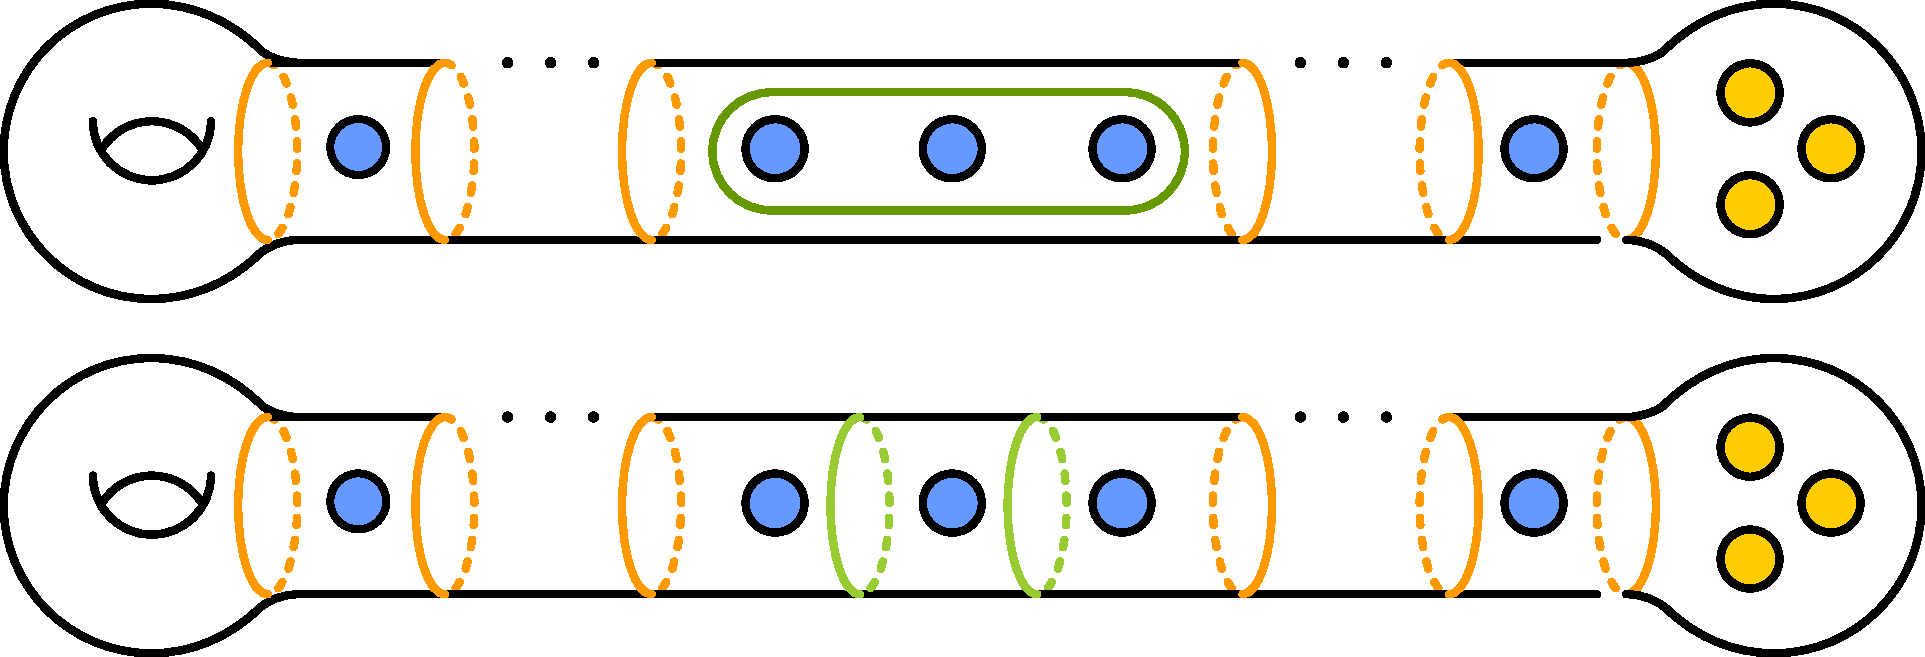
\includegraphics[width=.6\textwidth]{figures/cssmaxsimp5.pdf}
      \caption{(Top) A maximal simplex of submaximal dimension has multiple curves bounding 3-punctured disks.
      (Bottom) Replacing curves bounding a 3-punctured disk with a pair of curves results in a simplex of higher dimension.}
      \label{fig:cssmaxsimp5}
    \end{figure}

    Suppose that $p\geq 6$. Observe that a maximal dimension simplex has exactly one curve that bounds
    a 3-punctured disk, and simplices with multiple curves bounding 3-punctured disks may be maximal with respect to inclusion, but do not have maximal dimension.
    Observe that if $x$ bounds a 3-punctured disk then
    as in Figure \ref{fig:cssmaxsimp5} (top) we may choose a maximal (with respect to inclusion)
    simplex $\Delta$ of $\css S_{1,p}$ such that the region adjacency graph $\mathcal G_{\Delta}$ has 3 leaves,
    and
    the edge $e_x$ representing $x$ in $\mathcal G_{\Delta}$ is incident to a degree 3 vertex.
    Then by replacing $x$ with a pair $y,y'$ of curves as in Figure \ref{fig:cssmaxsimp5}
    we would obtain a maximal simplex of maximal dimension
    $$\Delta' = \Delta \cup \{x\} -\{y,y'\}.$$
    This shows a separating curve $x$ bounds a 3-punctured disk if and only if
    $x$ is contained in a maximal simplex $\Delta$ of submaximal dimension such
    that $\Delta-\{x\}$ is contained in a maximal simplex of maximal dimension.
    But then if $x$ bounds a 3-punctured disk, so does $\phi(x)$ for any $\phi \in \aaut \css S_{1,p}$.




    Suppose that $p = 4$ or $5$.
    Note that in this case any two distinct curves of the same type intersect,
    so that $\css S_{1,p}$ is colorable by curve type and in particular the ``extremal curve'' subcomplex
    $\mathcal E$ of curves bounding 3-punctured disks and $p$-punctured disks is connected and bipartitie.
    Assume to the contrary that there is $x$ bounding a 3-punctured disk such that $\phi(x)$ does not represent a 3-punctured disk for some automorphism $\phi \in \css S_{1,p}$.
    Then $\phi$ must swap the bipartition of $\mathcal E$
    Let $G < \aaut \css S_{1,p}$ be the subgroup generated by $\phi$ and $\mcg^{\pm} S_{1,p}$.
    We obtain a map $\rrho:G \to \Z/2$ with $\rrho(g)$ the generator of $\Z/2$ if $g$ exchanges the bipartition of $\mathcal E$.
    Then $\aaut \mathcal G_\Delta \cong \Z/2$ so that we have an exact sequence
    $$
    \begin{tikzcd}
      1 \arrow{r} &
      \mcg^{\pm} S_{1,p} \arrow{r} &
      G \arrow{r} &
      \Z/2 \arrow{r} &
      1
    \end{tikzcd}
    $$
    Then by Corollary \ref{cor:nomodextensions} it must be that $G \cong \Z/2 \times   \mcg^{\pm} S_{1,p}$.
    Then there an automorphism $\phi' \in \aaut \css S_{g,p}$ that is order 2 and commutes with $\mcg^{\pm} S_{1,p}$.
    If
    $x_0$ and $x_1$ are disjoint curves bounding a 3-punctured disk and a 4-punctured disk respectively,
    then
     there is a mapping class $\psi$ such that $\psi(x_0) = x_0$
    and $\psi(x_1) \neq x_1$, for example the half twist exchanging punctures on either side of $x_1$ along an arc disjoint from $x_0$.
    But this gives a contradiction:
    $$x_1=\phi'(x_0) =\phi'\psi(x_0) = \psi \phi' (x_0) = \psi(x_1)\neq x_1.$$
    It can only be that every automorphism preserves the type of curve.
\end{proof}

\begin{remark}
  Let $q$ be a puncture of $S_{g,p}$.
  Observe that the
  we have the projection
  $$
  \begin{tikzcd}
  \rho_q: \mathcal C(S_{g,p},q) \arrow{r}& \mathcal C S_{g,p-1}
  \end{tikzcd}
  $$
  restricts to the projection
  $$
  \begin{tikzcd}
    \rrho_q: \css S_{g,p} \arrow{r}& \csep S_{g,p-1}
  \end{tikzcd}
  $$
  since $\css S_{g,p}$ does not contain any curves bounding 2-punctured disks.
  So if $x$ is a separating curve of $S_{g,p-1}$
  the fiber $\rrho^{-1}_q(x) \subset \css S_{g,p}$ is
  isomorphic to a subforsest of the Bass-Serre tree $\mathcal T_x$
  given by the $x$ splitting of $\pi_1(S_{g,p-1},q)$,
  though $\rrho_q^{-1}\rrho_q (x) \subset \css S_{g,p}$ is not connected
  if $\rrho_q(x)$ is curve bounding a 2-punctured disk of $S_{g,p-1}$.
\end{remark}

\begin{definition}
  Let $\aaut(\css S_{g,p},q) < \aaut \css S_{g,p}$
  be the subgroup preserving the connected fibers of $\rrho_q$, so that $\phi \in \aaut (\css S_{g,p},q)$
  if
  $$
 \phi \left(   \rrho_q^{-1}\rrho_q (x) \right ) =   \rrho_q^{-1}\rrho_q ( \phi(x))
  $$
  for all $x$ such that $\rho(x)$ does not bound a 2-punctured disk.
\end{definition}

We recall the computation of the automorphism group of the separating curve complex due to Brendle, Margalit, and Kida in \cite{kida} and \cite{commensurations}.

\begin{theorem}
  \label{thm:sepcurvecomplex}
  The natural map
  $$ \mcg^\pm S_{g,p} \to \aaut \csep S_{g,p}$$
  is an isomorphism if $g=0,p\geq5$ or $g=1,p\geq3$ or $g=2,p\geq2$ or $g\geq 3$.
\end{theorem}

We show that automorphisms preserving the fibers of point forgetting projection $\rrho_q$
are in fact mapping classes.

\begin{lemma}
  The natural map
  $$ \mcg^\pm(S_{g,p},q) \to \aaut \css (S_{g,p},q)$$
  is an isomorphism if $g=0,p\geq6$ or $g=1,p\geq4$ or $g=2,p\geq3$ or $g\geq 3$.
  \label{lemma:cssfiberpres}
\end{lemma}

\begin{proof}
  Consider action by the Birman exact sequence.
  $$
  \begin{tikzcd}
  1 \arrow[r]&
  \pi_1(S_{g,p-1},q) \arrow[r] \arrow[d]&
  \mcg^{\pm}(S_{g,p},q)  \arrow{r}{f_q} \arrow{d}{\beta}&
  \mcg^{\pm}S_{g,p-1} \arrow{r}  \arrow{d}{\gamma} &
  1 \\
  1 \arrow[r]&
  \pi_1(S_{g,p-1},q) \arrow{r}{\alpha}&
  \aaut \css (S_{g,p},q)  \arrow{r}{\rrho^\ast_{q}}&
  \aaut \csep S_{g,p-1} \arrow{r}&
  1 \\
  \end{tikzcd}
  $$
  The diagram commutes by Lemma \ref{lemma:exact}, so we need only consider the exactness of the second row.
  Certainly any point push must move some strongly separating curve, so $\alpha$ is injective.
  By Theorem \ref{thm:sepcurvecomplex} we have $f_q \gamma = \rrho^\ast_q \beta$ is surjective,
  so that $\rrho^\ast_q$ must be surjective.
  As in the proof of Lemma \ref{lemma:exact}, $\mbox{image } \alpha \subset \ker \rrho^\ast_q$, since maps point pushing $q$
  around loops of $S_{g,p-1}$ act on the fibers of $\rrho_q$.

  Let $\phi \in \ker \rrho^\ast_q$.
  Suppose that $x \in \csep S_{g,p-1}$ is a curve that does not bound a 2-punctured disk.
  Then
  $$x=( \rrho^\ast_q \phi)(x)= \rho_q \phi (y)$$
  for any $y \in \rrho^{-1}_q(x)$.
  Then $\phi( \rrho^{-1}_q(x) ) = \rrho^{-1}_q(x)$
  so that $\phi$ is determined by its action on each $\rrho^{-1}_q(x)$.
  But $\rrho^{-1}_q(x)$ is $\pi_1(S_{g,p-1},q)$ equivalently isomorphic to the Bass Serre tree $\mathcal T_x$,
  and since $\ker \rrho^\ast_q$ acts on $\mathcal T_x$ it follows by Theorem \ref{thm:bassserre} that
  $\ker \rrho^\ast_q$ acts on $\mathcal T_x$ as $\pi_1(S_{g,p-1},q)$.
  Then we may compose $\phi$ with a push map to assume that $\phi(y)=y$
  for any strongly separating curve $y$ in $S_{g,p}$ that bounds a 3-punctured disk containing $q$.
  Then if $y$ in $S_{g,p}$ bounds a 3-punctured disk containing $q$.
  Let $\Sigma$ be any collection of curves disjoint from $y$ such that $y$ bounds the only
  3-punctured disk disjoint from every curve of $\Sigma$.
  No curve of $\Sigma$ bounds a 3-punctured disk containing $q$, so $\phi$
  fixes $\Sigma$, and it must be that $\phi(y)=y$.
  But then
   $$\mbox{image } \alpha = \ker \rrho^\ast_q.$$
  Then the rows of the commutative diagram are exact and by the Five Lemma the map $\beta$ is an isomorphism.
\end{proof}

\begin{definition}
  Let $\aaut^\rrho \css S_{g,p} < \aaut \css S_{g,p}$ be the subgroup that permutes the connected fibers of the point forgetting map, so
  $\phi \in \aaut^\rrho \css S_{g,p}$ if there is a permutation $\sigma$ of the punctures $P$ such that
  $$
   \phi \left( \rrho_q^{-1}\rrho_q(x) \right ) =  \rrho_{\sigma(q)}^{-1}\rrho_{\sigma(q)}( \phi(x))
  $$
  for every puncture $q \in P$ and curve $x \in \css S_{g,p}$ such that $x$ does not bound a 3-punctured disk containing $q$.
\end{definition}

\begin{corollary}
  The natural map
  $$ \mcg^\pm S_{g,p} \to \aaut^\rrho \css S_{g,p}$$
  is an isomorphism if $g=0,p\geq6$ or $g=1,p\geq4$ or $g=2,p\geq3$ or $g\geq 3$.
  \label{cor:cssallfiberspres}
\end{corollary}

\begin{proof}
  Let $\phi \in \aaut^\rrho \css S_{g,p}$ and let $\sigma$ be the associated permutation of the punctures.
  Then there is $\psi \in \mcg^\pm S_{g,p}$ such that $\psi^{-1}(q) = \sigma(q)$ for every puncture $q \in P$.
  So $\psi \phi$ preserves $\rrho_q^{-1}\rrho_q(x)$ for  every $x \in \css S_{g,p}$ and some $q \in P$.
  Then $\psi \phi \in \aaut \css  (S_{g,p},q)$ so by Lemma \ref{lemma:cssfiberpres}
  it must be that $\phi$ is induced by a mapping class.
\end{proof}

\begin{remark}
  We will use a similar technique to Chapter \ref{chap:birman} to show that $\aaut \css S_{g,p}$
  always permutes the fibers of the puncture forgetting map $\rrho$ if $S_{g,p}$ has sufficiently high complexity by
  showing $\aaut \css S_{g,p}$ permutes the coloring of an arc complex associated to the fibers of $\rrho$.
\end{remark}

\begin{definition}
  Define the strongly separating pointed arc complex
  $\mathcal A^{ssep} S_{g,p}$
  to be the complex of homotopy classes of 3-punctured disks
  and pointed loops
  in $S_{g,p}$ whose regular neighborhood
  is bounded by strongly separating curves.
  Two loops or punctured disks are adjacent in
  $\mathcal A^{ssep} A S_{g,p}$ if their homotopy classes
  have disjoint representatives including endpoints.
  \label{def:strongptarc}
\end{definition}

\begin{lemma}
  \label{lem:csstoass}
  Automorphisms of $\aaut \css S_{g,p}$ induce automorphisms of $\mathcal A^{ssep} S_{g,p}$.

  There is an $\mcg^\pm S_{g,p}$ equivariant homomorphism
  $$\aaut \css S_{g,p} \to \aaut \mathcal A^{ssep} S_{g,p}.$$
\end{lemma}
\begin{proof}
  The proof is similar to that of Lemma \ref{lemma:annulus}.
  Suppose that $\phi \in \aaut \css$.

  If $x$ is a strongly separating loop, then the boundary of a regular neighborhood
  of $x$ is two strongly curves $y,y'$ that cobound a punctured annulus of $S_{g,p}$.
  The curves $y,y'$ cobound a punctured annulus if and only if there is
  a maximal dimension simplex $\Delta$ of $\css S_{g,p}$ such that in the adjacency graph $\mathcal G_\Delta$,
  the edges corresponding to $y$ and $y'$ are incident to the same degree 2 vertex $v_x$.
  Lemma \ref{thm:cssgraphs} guarantees that $\phi(y)$ and $\phi(y')$ cobound
  a regular neighborhood of a strongly separating loop that we define to be $\hat \phi(x)$.

  If $x$ is a 3-punctured disk, then Lemma \ref{thm:csstype} guarantees that
  its bounding curve $y$ has $\phi(y)$ bound a 3-punctured disk $\hat \phi (x)$.

  Then $\hat \phi$  is simplicial since  loop or 3-punctured disk of $S_{g,p}$
  are disjoint if and only if their above characterizing-curves span a simplex in $\css S_{g,p}$.
  So we have a homomorphism by $\phi \mapsto \hat \phi$.
\end{proof}

\begin{lemma}
  $\mathcal A^{ssep}  S_{g,p}$ is uniquely colorable for $g\geq 3$ or $g\geq 2, p\geq 4$.
  \label{lem:asscolor}
\end{lemma}

\begin{proof}
The proof is similar to the proof of Lemma \ref{lemma:paint},
though the arc complex has only strongly separating loops and 3-punctured disks,
so the similar argument requires a higher complexity surface.

Again we argue that there are color forcing paths between nests,  as in Example \ref{example:nests}.
But if $V$ and $V'$ are nests respectively parallel to curves that intersect, the argument
in Example \ref{example:nests} would require at least 6 punctures.
We consider the cases of different complexities separately.
Since connected bipartite graphs are uniquely colorable we assume that $p\geq 3$.

\emph{Case 1.} Assume that $g \geq 3$.

Fix a puncture order $\sigma: P \to \{1, \ldots, p\}$ and a separating curve $x$ of $S_g$
and let $N$ be a $\sigma$-nest of $S_{g,p}$ parallel to $x$.
Let $V=\{N_i\}_{i =1}^p$ be the corresponding clique of $\css S_{g,p}$.
Let $z$ be a regular neighborhood of the spine of $N$, so that $z$ is $p$-punctured disk
whose bounding curve intersects each rib $N_i$ of the nest with geometric intersection 2.
Choose any collection $\Sigma$ of nonseparating curves whose Dehn twists generate
$\mcg^\pm (S_{g,p},z)$,
the mapping classes fixing $z$ pointwise.
Then let $H$ be the generating set for $\mcg^\pm S_{g,p}$
given by twists about the curves of $\Sigma$
and the half-twist about the vertabrae of the nest $N$.

\begin{figure}[h!]
  \centering
  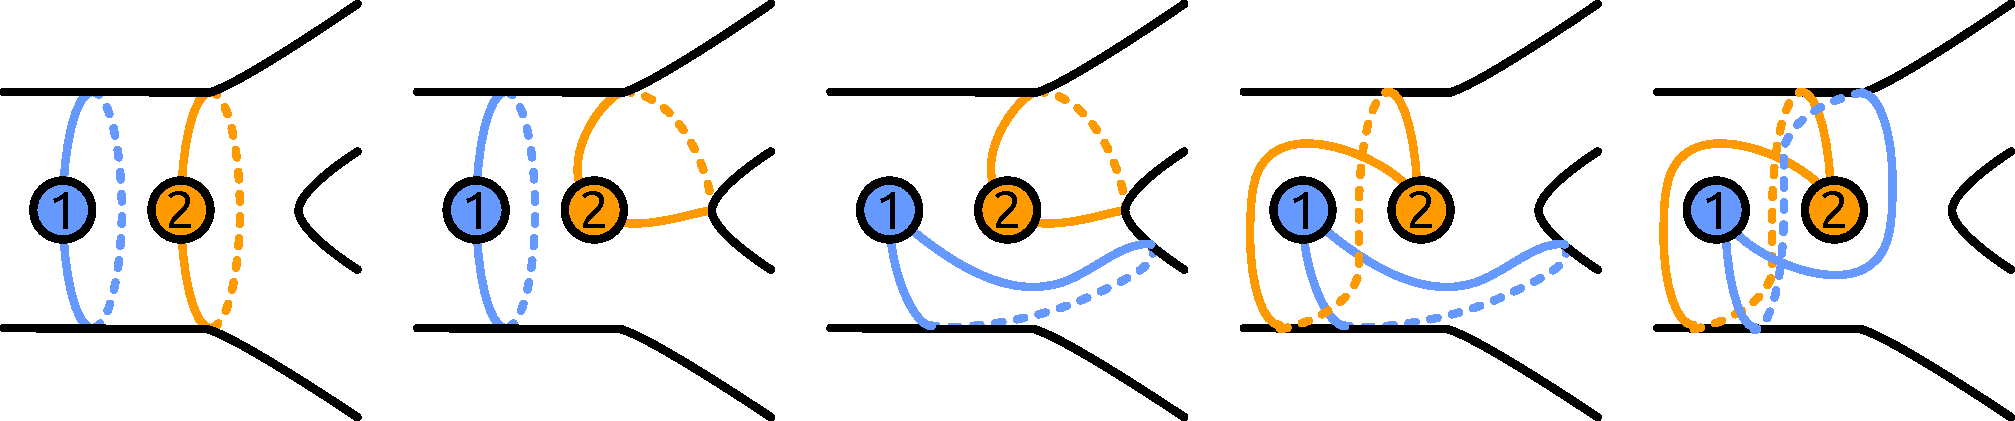
\includegraphics[width=\textwidth]{figures/strongbraid1.pdf}
  \caption{A color forcing sequence between two parallel loops and their braid.}
  \label{fig:strongbraid1}
\end{figure}

Figure \ref{fig:strongbraid1} shows a color forcing sequence between
the ribs $N_i$ and $N_{i+1}$ and their image under the half-twist about a vertebra of $N$.

If $x,x'$ are disjoint strongly separating spheres then as in \ref{example:nests}
these is a color forcing sequence between $\sigma$-nests parallel to $x$ and $x'$.
It must be that $V$ forces a coloring on its orbit $\mcg^{\pm} S_{g,p} \cdot V$.
Observe that any 3-punctured disk of $S_{g,p}$ is disjoint from $p-3$
loops in $\mcg^{\pm} S_{g,p} \cdot V$.
Then a $V$ also forces a coloring on every 3-punctured disk.
A coloring on a loop bounding a $k$-punctured disk
is determined by $p-k$ loops of $\mcg^{\pm} S_{g,p} \cdot V$
and loops bounding $k-1$-, $k-2$-, $\ldots$, and $4$-punctured disks and a 3-punctured disk.
We conclude by induction that $V$ forces a coloring on $\mathcal A^{ssep} S_{g,p}$.


\emph{Case 2.} Assume that $g=2$ and $p \geq 4$.

\begin{figure}[h!]
  \centering
  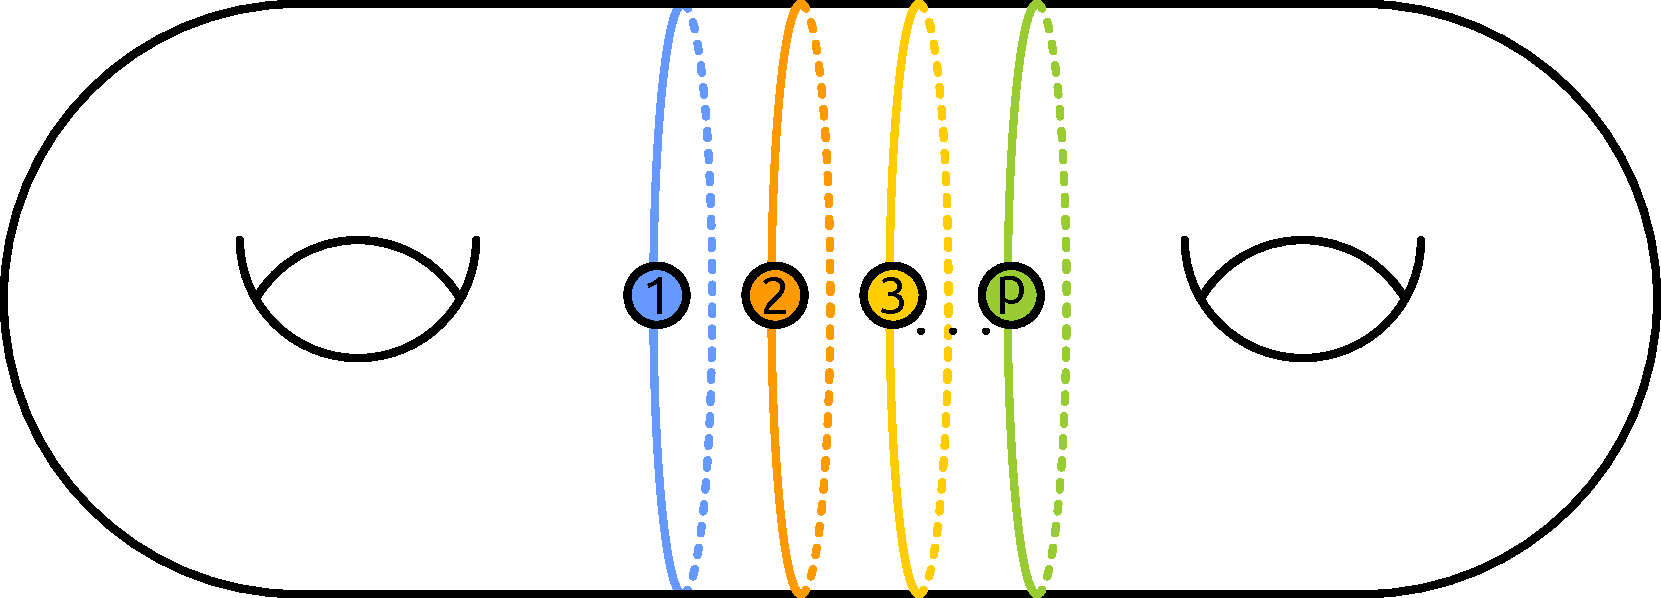
\includegraphics[width=.5\textwidth]{figures/strongnest.pdf}
  \caption{A base nest of strongly separating curves.}
  \label{fig:strongnest}
\end{figure}

Fix a nest as in Figure \ref{fig:strongnest}.
Let $V=\{N_i\}$ be the corresponding simplex of $\mathcal A^{ssep} S_{g,p}$.
Certainly $V$ requires $p$ colors to color.
Let $H$ be the generating set for $\mcg S_{g,p}$ consisting of the braids about
the vertebrae of $N$ and the Dehn twists about the nonseparating curves shown in Figure \ref{fig:strongtwists}.

\begin{figure}[h!]
  \centering
  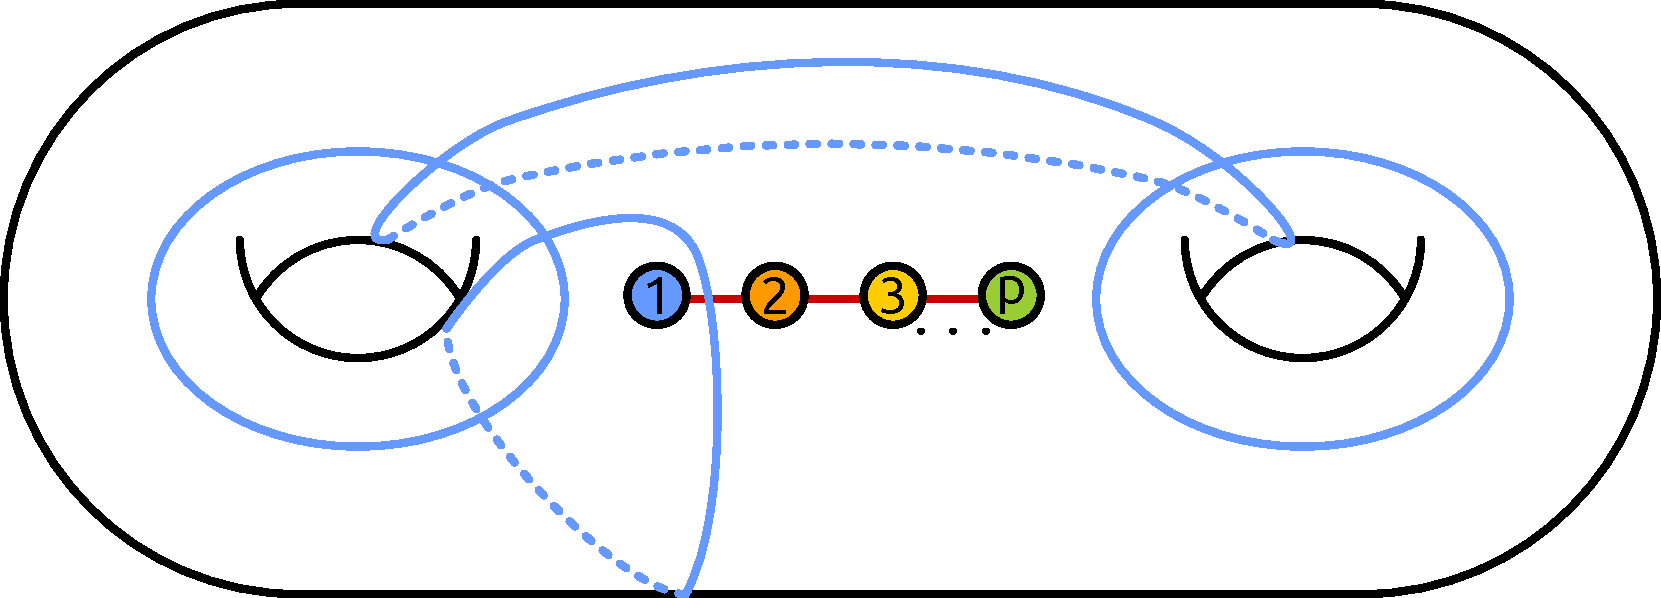
\includegraphics[width=.5\textwidth]{figures/strongtwists.pdf}
  \caption{The mapping class group is generated by Dehn twists about these nonseparating curves
  and braiding about the vertebrae of the nest, shown in red.}
  \label{fig:strongtwists}
\end{figure}

We first show $V$ forces a coloring on $T_{v_i} \cdot V$ for a half-twist $T_{v_i}$ about the $i^{\mbox{th}}$ vertebra $v_i$ of nest $N$.
Figure \ref{fig:strongtwist} (left) shows that $N_i, \ldots, N_{i+3}$ force a coloring on $v_i \cdot N_i, v_i \cdot N_{i+1}$.
A similar arugment concludes $N_i, \ldots, N_{i+3}$ force a coloring on $v_{i+2} \cdot N_i, v_{i+2} \cdot N_{i+1}$.
Figure \ref{fig:strongtwist} (right) shows that $N_i, \ldots, N_{i+3}$ force a coloring on $v_{i+1} \cdot N_i, v_{i+1} \cdot N_{i+1}$.

\begin{figure}[h!]
  \centering
  \hspace*{\fill}
{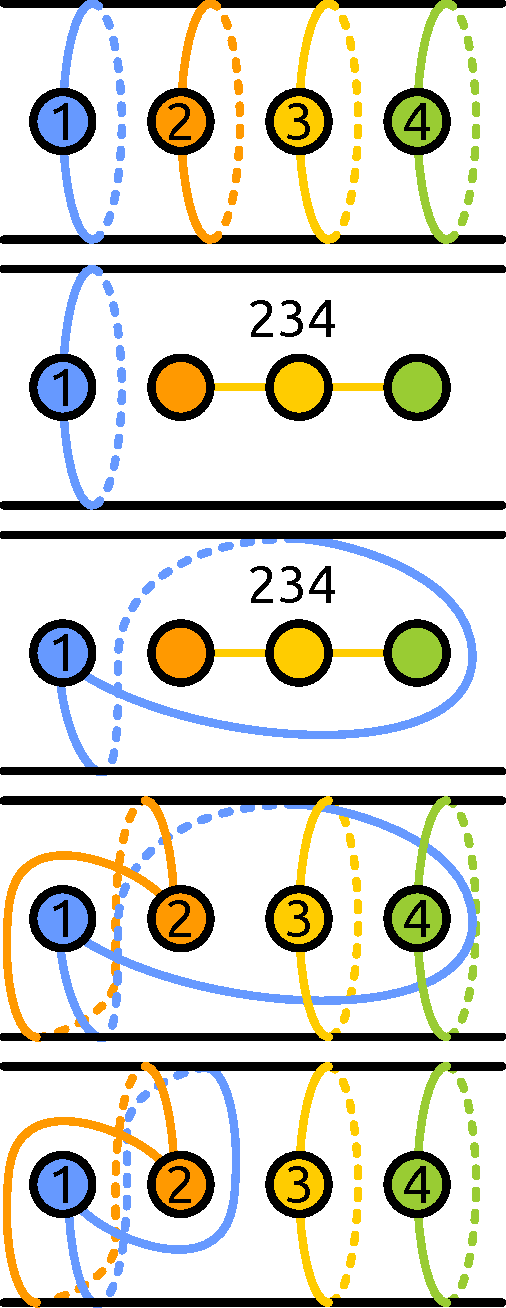
\includegraphics[width=.2\textwidth]{figures/strongtwist.pdf}} \hfill {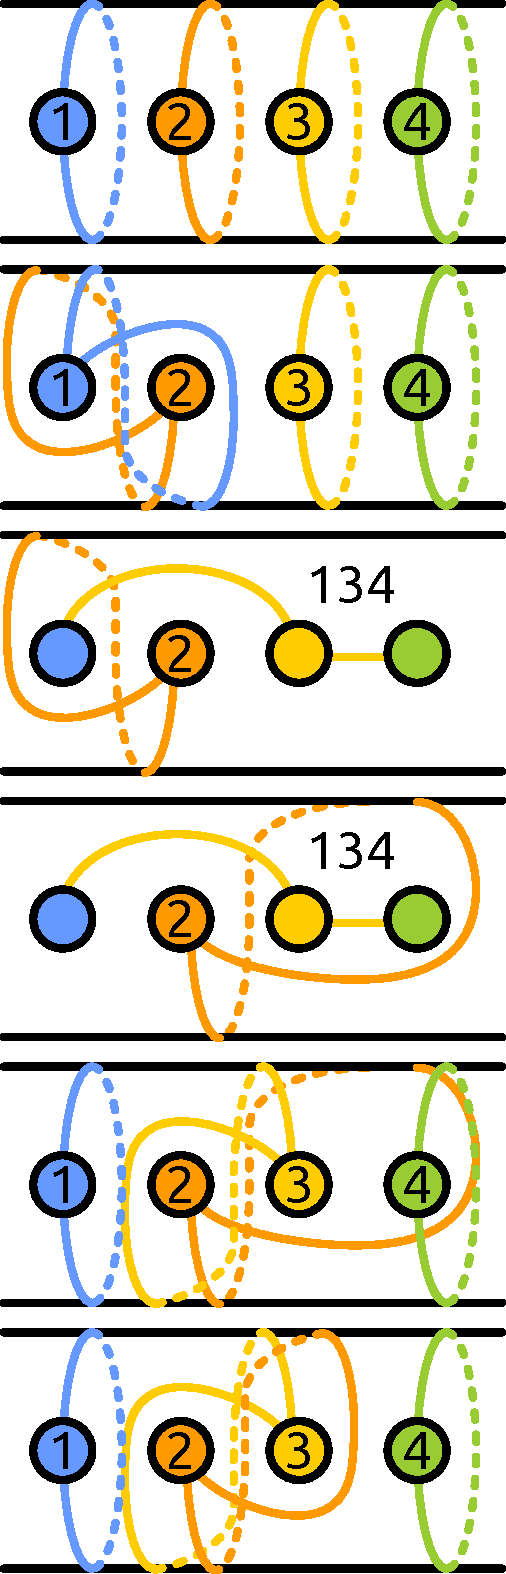
\includegraphics[width=.2\textwidth]{figures/strongtwist2.pdf}}
\hspace*{\fill}
  \caption{A nest forces a coloring on its image under braids about the vertebrae of the nest.}
  \label{fig:strongtwist}
\end{figure}




\begin{figure}[h!]
  \centering
  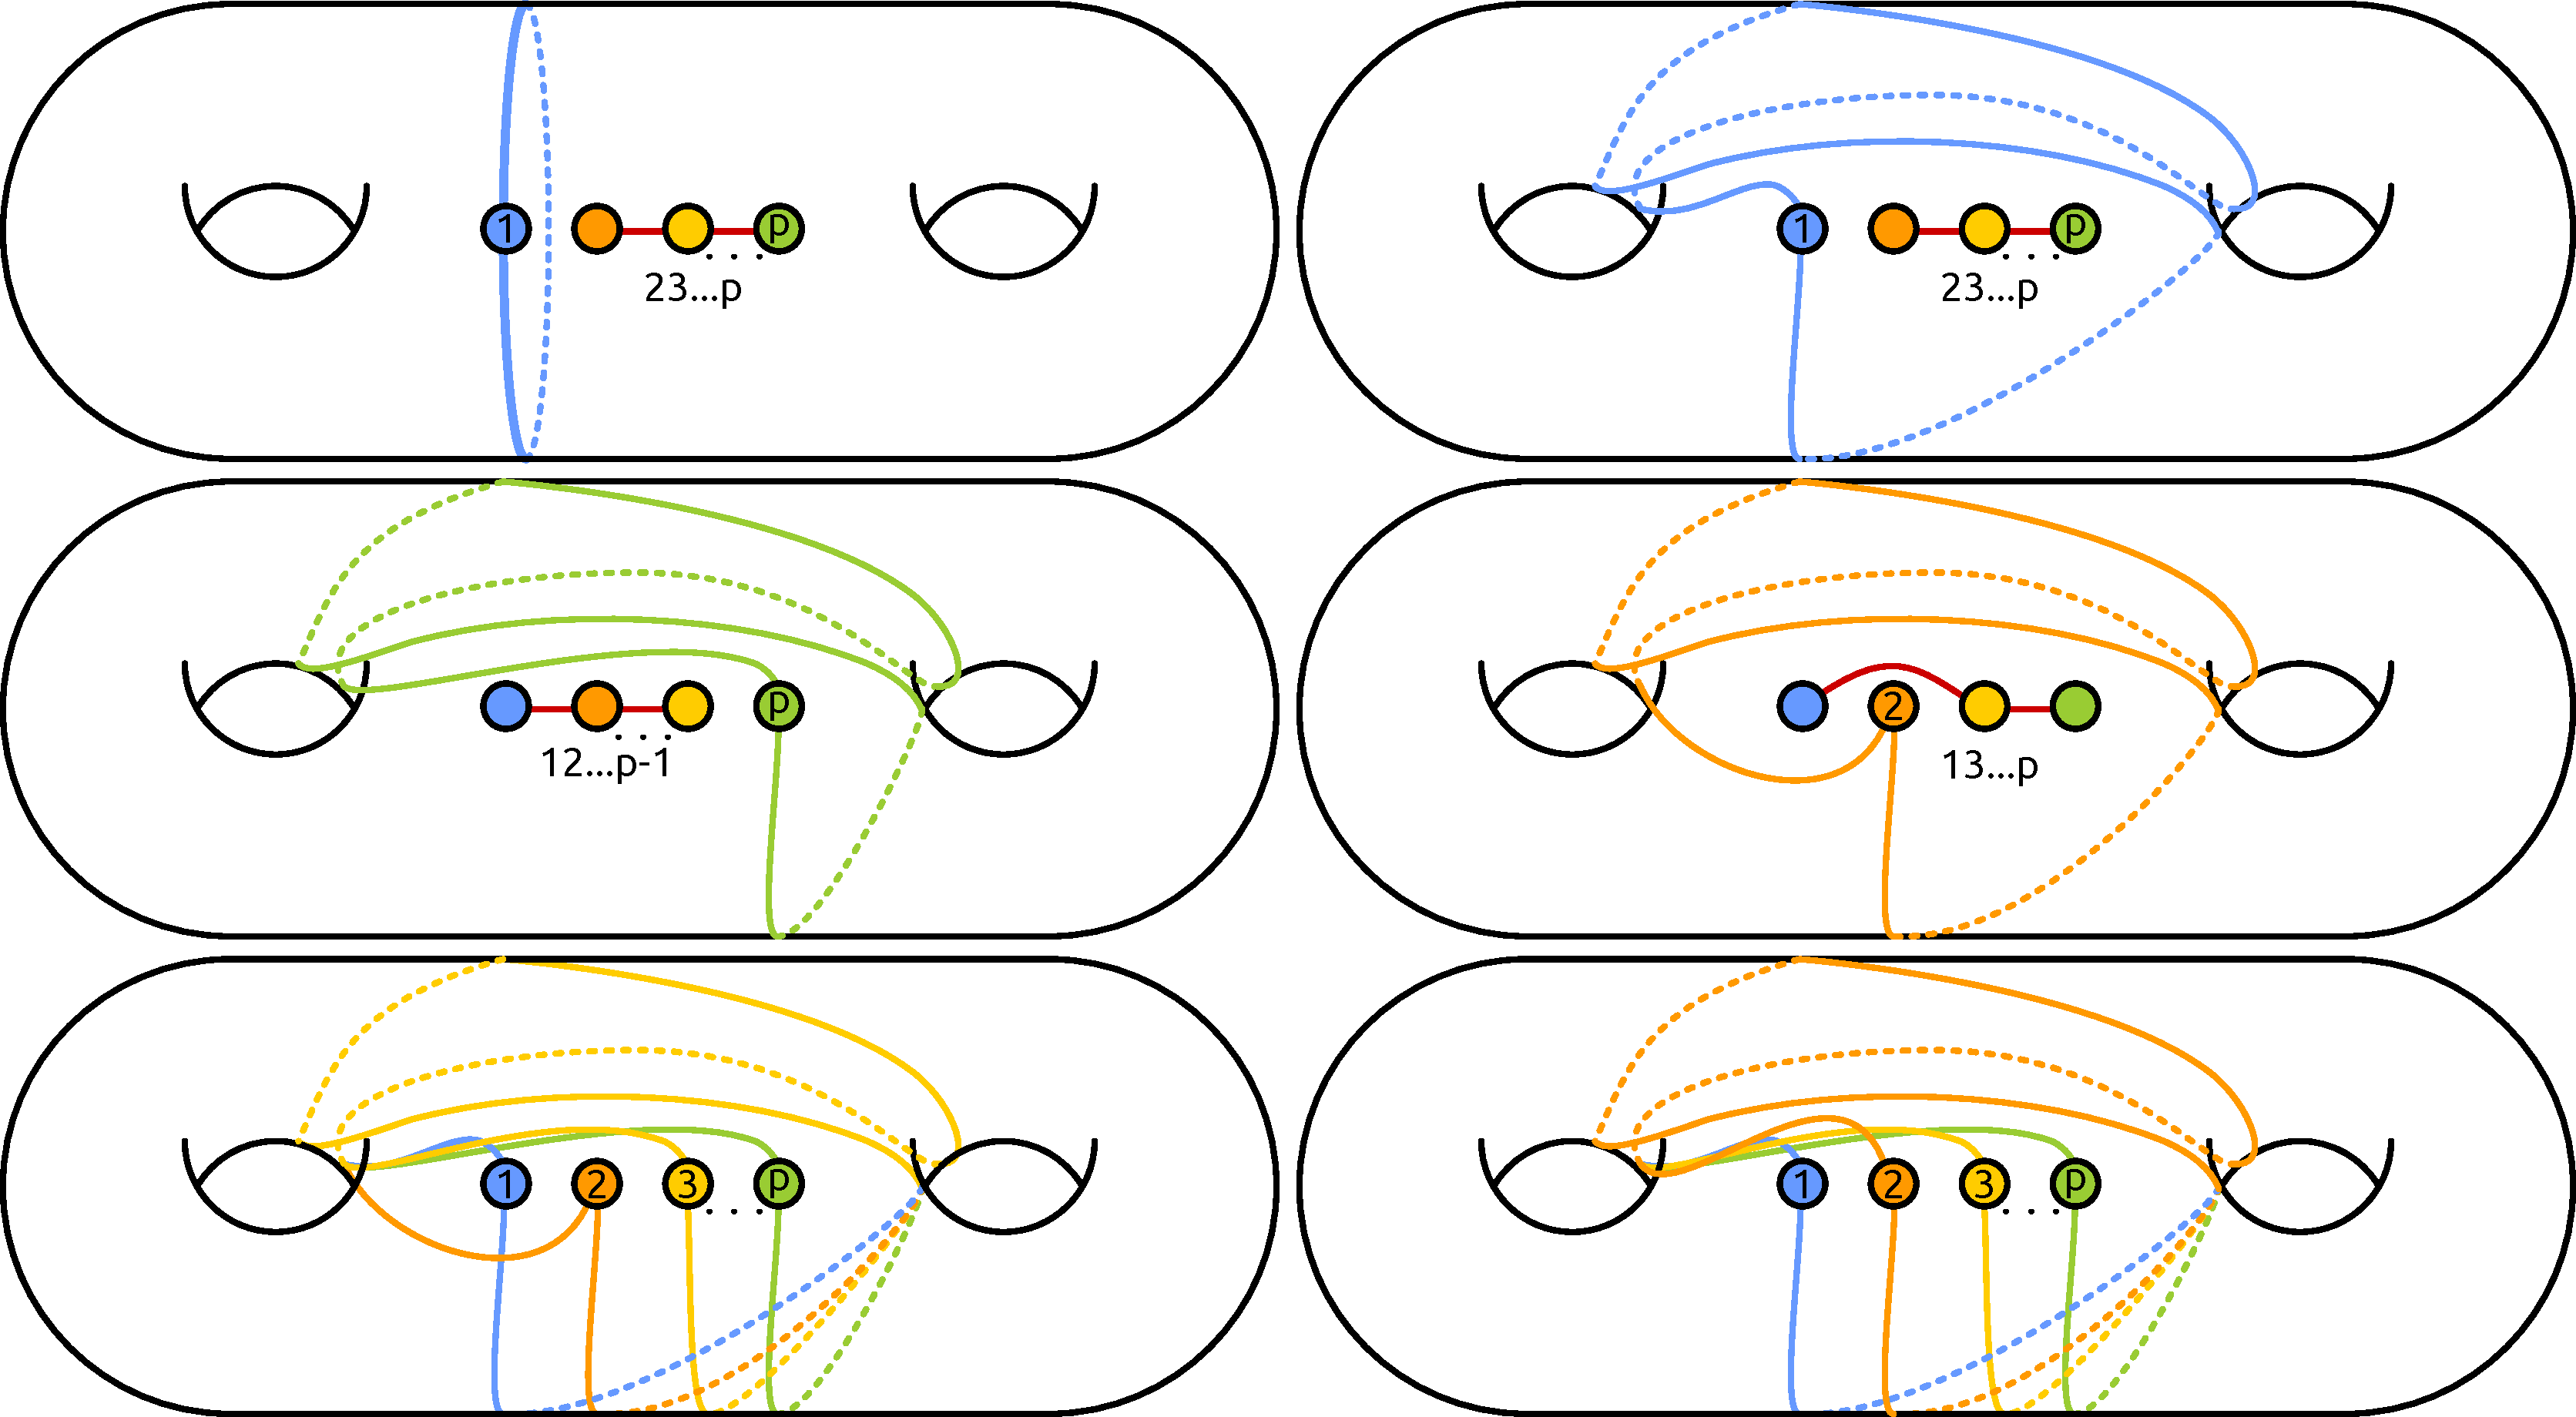
\includegraphics[width=\textwidth]{figures/strongdehn.pdf}
  \caption{The loops of $V$ force a coloring on their image $T_\alpha \cdot V$ under the Dehn twist $T_\alpha$
  by considering color forcing sequence passing through loops contained in $p$-punctured disks of $S_{2,p}$.}
  \label{fig:strongdehn}
\end{figure}

It remains only to be seen that $V$ forces a coloring on its image under Dehn twists of $H$.
Of the Dehn twists described by Figure \ref{fig:strongtwists}
only one, say $T_\alpha$, fixes fewer than $p-1$ loops of $V$.
As in Example \ref{example:nests}, $V$ forces a coloring on loops parallel to punctured
disks that are the regular neighborhoods of vertebrae and half-twists of vertebrae,
that force colorings on $p-3$ size subsets of $T_\alpha \cdot V$.
Since $p-3$ size subsets of $T_\alpha \cdot V$ cover $T_\alpha \cdot V$,
we have that $V$ forces a coloring on $T_\alpha \cdot V$.
So $V$ forces a coloring on $\mathcal A^{ssep} S_{2,p}$ by Lemma \ref{putmancolor}.

% \emph{Case 2.} Assume that $g=1$ and $p \geq 6$.
\end{proof}



\begin{remark}
  The unique coloring of
  $\mathcal A^{ssep}  S_{g,p}$ fails for the lowest complexity cases.
  In particular the loops of $\mathcal A^{ssep}  S_{2,3}$ and
  $\mathcal A^{ssep}  S_{1,4}$ are disconnected,
  and $\mathcal A^{ssep}  S_{1,5}$ may be colored by 3 topolocial curve types, rather
  than the 5 punctures.
\end{remark}

\begin{proof}[Proof of Theorem \ref{thm:css}]
  We consider only the cases
  $$(g,p) \in \{(2,4),(3,2),(3,3),(4,2)\}$$
  which are undecided in \cite{bowditch}
  By Lemma \ref{lem:csstoass}
  any automorphism $\phi \in \aaut \css S_{g,p}$
  induces an automorphism $\phi_\ast$ of $\mathcal A^{ssep} S_{g,p}$,
  so by Lemma \ref{lem:asscolor} there is some permutation $\sigma$ of the punctures such that $\phi$
  permutes the puncture-coloring of $\mathcal A^{ssep} S_{g,p}$ by $\sigma$.
  By composing $\phi$ with a mapping class permuting the punctures by $\sigma^{-1}$,
  we may assume that $\phi_\ast$ fixes the puncture-coloring of $\mathcal A^{ssep} S_{g,p}$.

  Suppose that $x' \in \rho_q^{-1} \rho_q (x)$ for $x \in \css S_{g,p}$ such that $x$ does not bound a 3-punctured disk containing $q$.
  Then $\rho_q^{-1} \rho_q(x)$ is isomorphic to the Bass Serre tree $\mathcal T_x$
  and in particular connected.
  Then there is a path $x=x_0,\ldots,x_n=x'$ with $x_i$ and $x_{i+1}$ cobounding an annulus punctured by $q$.
  But then $\phi(x_0),\ldots,\phi(x_n)$ is a path of curves with $\phi(x_i)$ and $\phi(x_{i+1})$ cobounding annuli punctured by $q$.
  So $\phi(x') \in \rho_q^{-1} \rho_q( \phi(x))$.
  But then $\phi \in \aaut^\rrho \css S_{g,p}$.
  From Corollary \ref{cor:cssallfiberspres} we conclude that $\phi$ is induced by a mapping class.
\end{proof}

\section{The Low Complexity Cases}
\label{sect:leftovers}

\begin{remark}
  In \cite{meta}
  Brendle and Margalit %\cite{}
  demonstrate that automorphisms of subgraphs of the curve complex $\mathcal C S_{g}$
  can often be extended to the full complex $\mathcal C S_{g}$ by \emph{sharing pairs}
  where two curves bound subsurfaces that intersect to give a third curve.
  The action of automorphisms on the sharing pair is then used to extend the automorphism to the shared curve.

  In light of Theorem \ref{thm:sepcurvecomplex}
  automorphisms of  $\css S_{g,p}$ need only be extended to curves bounding 2-punctured disks.
  Brendle and Margalit give a combinatorial characterization of sharing pairs in terms of
  five additional curves beyond the sharing pair.
  Their technique can also be used to verify that $\aaut \css S_{g,p}$ is the mapping class group
  in all high genus cases, but in low complexity cases there simply is not enough
  room to use their techniques to demonstrate if sharing pairs are preserved.
  However, a similar technique allows us to give reductions between computations of $\aaut \css S_{g,p}$
  for different genus $g$ and number of punctures $p$.
\end{remark}

\begin{definition}
  Let $z$ be curve bounding a 2-punctured disk.
  When $p\geq 4$ define a \emph{sharing pair} of $S_{g,p}$ for $z$ to be a pair of curves $\{x,x'\}$
  both of that bound 3-punctured disks containing $z$ and such that $x$ and $x'$ have geometric intersection 2.
  If $p =3$ we instead demand that $x$ and $x'$ have geometric intersection 4.
  If $p=2$ we instead demand that $x$ and $x'$ bound $S_{1,3}$s containing $z$ and have either geometric intersection 2,
  or $x$ and $x'$ have geometric intersection 4 and there is a curve $x''$ that bounds an $S_{1,1}$ on the same side as $z$ of $x$ and $x'$.

  Let  $\mathcal P'_z$ be the sharing pair graph defined as follows.
  Let the vertices of $\mathcal P'_z S_{g,p}$ be the sharing pairs for $z$.
  Two sharing pairs for $z$ are adjacent if there is a curve $y$ bounding an $S_{1,1}$
  that lies on the opposite side of $z$ for each curve in each sharing pair.
\end{definition}

\begin{lemma}
  Let $z$ be a curve bounding a 2-punctured disk in $S_{g,p}$.
  The sharing pair graph $\mathcal P'_z$
  is connected if $g\geq 1, p\geq 5$, or $g\geq2, p\geq 3$, or $g\geq3, p\geq 2$.
  \label{lemma:cogenussharepair}
\end{lemma}

\begin{proof}
  We appeal to Putman's Lemma \ref{lemma:putman} using $\mcg S_{g,p}$ and
  considering cases based on the genus and number of punctures,
  since our definition of sharing pairs is surface dependent.
  Since in every case $\mcg S_{g,p}$
  acts transitively on the sharing pairs of $S_{g,p}$ (except for $p=4$),
  it suffices to choose a generating set $H$ and sharing pair $v$ for the 2-punctured disk $z$
  and show that
  for each $h \in H$ there is a sequence of sharing pairs $\{x_i,x'_i\}$
  from $h\cdot v$ to $v$ such that for each $i$ there is an $S_1,1$
  disjoint from $x_{i},x'_i,x_{i+1},$ and $x'_{i+1}$.

  \emph{Case 1.} Consider $g\geq 1$ and $p\geq 5$.

  \begin{figure}[h!]
    \centering
    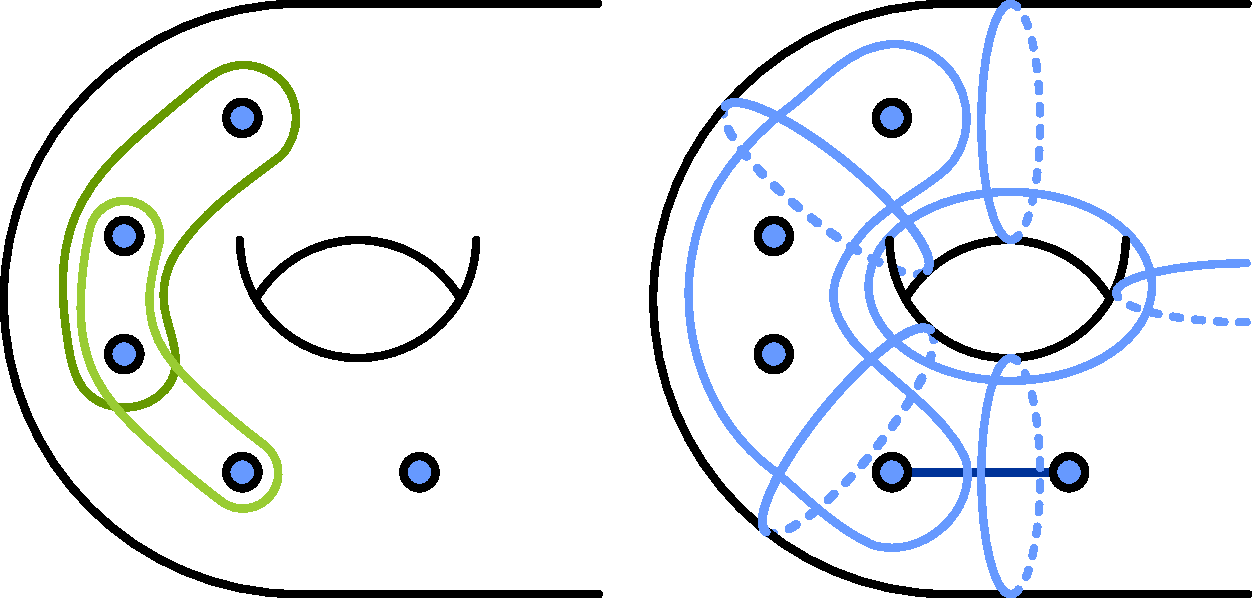
\includegraphics[width=.5\textwidth]{figures/handlecompliment.pdf}
    \caption{(Left) A sharing pair. (Right)Curves for twists  generating $\mcg$.}
    \label{fig:csshandlecomp1}
  \end{figure}

  \begin{figure}[h!]
    \centering
    \includegraphics[width=.5\textwidth]{figures/handlecompliments1b.pdf}
    \caption{(Left) Braiding points about a minimally intersect arc $\beta$ moves $v$ disjointly from an $S_{1,1}$.
    (Right) A twist about a nonseparating arc intersecting one curve of the sharing pair.
    The resulting sharing pair is distance 2 from $v$.}
    \label{fig:csshandlecomp1b}
  \end{figure}

  Fix a sharing pair $v={x_0,x'_0}$ as in Figure \ref{fig:csshandlecomp1} left.
  Let $H$ be the generating set for $\mcg (S_{g,p},z)$ given by Dehn twists about the curves shown
  in Figure \ref{fig:csshandlecomp1} right.
  In particular $H$ may be taken to consist of Dehn twists about curves disjoint from
  the sharing pair $v$,
  the twist $T_a$ about a nonseparating curve $a$ intersecting $x_0$ twice and $x'_0$ zero times,
  the twist $T_{a'}$ about a curve $a'$ intersecting $x'_0$ twice and $x_0$ zero times,
  the half twist $T_\alpha$ such that $T^2_\alpha$ is the Dehn twist about the boundary of the 4-punctured disk containing $v$
  (shown in green in Figure \ref{fig:csshandlecomp1}),
  and a half twist $T_\beta$ swapping a puncture in $x_0$
  with a puncture out of $v$
  about an arc $\beta$ intersecting $x_0$ once and $x'_0$ zero times.
  Then $T_\alpha$ swaps $x_0$ and $x_0'$, but fixes $v$.
  In Figure \ref{fig:csshandlecomp1b} (left) we see that
  the half twist $T_\beta$ has $T_\beta \cdot v = \{x_0', T_\beta x_0 \}$
  that is contained in a 5-punctured disk with $v$ so that $v$
  and $T_\beta \cdot v$ are distance 1 in $\mathcal P'_z$.
  In Figure \ref{fig:csshandlecomp1b} (right) we see that
  $T_a \cdot v = \{x_0', T_a x_0 \}$
  that is contained in a 5-punctured disk with $T_\beta v$ so that $v$
  and $T_a \cdot v$ are distance 2 in $\mathcal P'_z$.
  The case of $T_{a'}$ is similar.



  \emph{Case 2.} Consider $p=4$ and $g \geq 2$.

  \begin{figure}[h!]
    \centering
    \includegraphics[width=.8\textwidth]{figures/handlecompliment2.pdf}
    \caption{(Left) A half twist about the green curve and twists about the blue generate $\mcg S_{g,p}$. (Right) Any two of these are a sharing pair.}
    \label{fig:csshandlecomp2}
  \end{figure}

  When there are 4 punctures we have two topological types of sharing pairs:
  those with intersection 2 and those with intersection 4.
  But as in Figure \ref{fig:csshandlecomp2}
  any intersection 4 pair is contained with an intersection 2 pair in an $S_{1,4}$
  disjoint from an $S_{1,1}$.
  So all of $\mathcal P'_z$ is connected to the orbit of $v$.
  We may generated $\mcg S_{g,p}$ by a half-twist exchanging the non-$z$ punctures, but fixing $v$
  and Dehn twists about a set separating curves as in Figure \ref{fig:csshandlecomp2}.
  The twist of $xfor the the_0$ about a separating curve disjoint from $x'_0$ and intersecting $x_0$ twice
  is also contained with $x_0$ and $x'_0$ in the complement of an $S_{1,1}$.


  \emph{Case 3.} Consider $p=3$ and $g \geq 2$.

  \begin{figure}[h!]
    \centering
    \includegraphics[width=.4\textwidth]{figures/handlecompliment3.pdf}
    \caption{(Top) A sharing pair and a generating set. (Middle,Bottom)
    The images of sharing pair $v$ under generators are contained with $v$ in the complement of an $S_{1,1}$.}
    \label{fig:csshandlecomp3}
  \end{figure}

  The case is similar. By choosing a generating set $H$ for $\mcg (S_{g,p},z)$
  consisting
  of Dehn twists about nonseparating curves
  that intersect the sharing pair minimally as in Figure \ref{fig:csshandlecomp3}, we can ensure
  that $h \cdot v$ is always distance 1 from $v$.




  \emph{Case 4.} Consider $p=2$ and $g \geq 3$.

  Figure \ref{fig:csshandlecomp4} shows a base sharing pair $v$
  and a set of nonseparating curves whose Dehn twists $H$ generate the mapping class group fixing $z$.
  Figure \ref{fig:csshandlecomp4b} shows a length 5 path in $\mathcal P'_z$
  that contains the image of $v$ under $H$.
for the the
  \begin{figure}[h!]
    \centering
    \includegraphics[width=\textwidth]{figures/handlecompliment4.pdf}
    \caption{(Right) A set of nonseparating curves whose Dehn twists generate the mapping class group fixing $z$. (Left)A sharing pair.}
    \label{fig:csshandlecomp4}
  \end{figure}

  \begin{figure}[h!]
    \centering
    \includegraphics[width=\textwidth]{figures/handlecompliment4b.pdf}
    \caption{A length 5 path in $\mathcal P'_z$
    that contains the image of $v$ under $H$.
    In the top row there are sharing pairs, giving vertices of $\mathcal P'_z$.
    In the bottom row are $S_{1,1}$s disjoint from both sharing pairs above,
    giving edges of $\mathcal P'_z$.
    }
    \label{fig:csshandlecomp4b}
  \end{figure}

  The case is similar to Case 2, but the paths in $\mathcal P'_z$ are longer.
  Figure \ref{fig:csshandlecomp4} gives a base sharing pair $v$ and a generating set.
  Figure \ref{fig:csshandlecomp4b} shows a path in $\mathcal P'_z$ containing the image
  of $v$ under the generating set.
\end{proof}


\begin{lemma}
  If the natural map
  $$
    \mcg S_{g-1,p+1} \to \aaut \css S_{g-1,p+1}
  $$
  is an isomorphism, then so is
  $$
    \mcg S_{g,p} \to \aaut \css S_{g,p}
  $$
  provided
  $g\geq 1, p\geq 5$, or $g\geq2, p\geq 3$, or $g\geq3, p\geq 2$.
  \label{lemma:s23tos14}
\end{lemma}

\begin{proof}
  Assume that $\aaut \css S_{g-1,p+1} \cong \mcg^pm S_{g-1,p+1}$.
  Let $\phi \in \css S_{g,p}$.
  Let $z$ be a curve bounding a 2-punctured disk of $S_{g,p}$.
  Let $\{x,x'\}$ be a sharing pair for $z$ with $x,x' \in \aaut C_ss S_{g,p}$.
  Then there is a curve $y \in \aaut \css S_{g,p}$ on the large side of $x$ and $x'$ and such that $y$ bound an $S_{1,1}$ and an $S_{g-1,p+1}$ that contains $x$ and $x'$.
  By Lemma \ref{thm:csstype} $\phi(y)$ also bounds an $S_{1,1}$,
  so without loss of generality we may compose $\phi$ with a mapping class so that $\phi$ fixes $y=\phi(y)$.
  Then considering $y$ as if it were puncture for the large side of its complement, note that the link of $y$
  contains a subcomplex $$\mathcal L_y \cong \css S_{g-1,p+1}$$
  Then by hypothesis $\phi$ acts on $\mathcal L_y$ as a mapping class,
  so there is $\psi \in \mcg^\pm S_{g,p}$ such that
  $$\psi(y') = \phi(y')$$
  for every $y' \in \mathcal L_y$.
  In particular the $\phi(x),\phi(x')$ are the homeomorphic image of $x,x'$ so that
  $\phi(x),\phi(x')$ must be a sharing pair for a 2-punctured-disk-bounding curve we denote $\hat \phi(z)$.
  Further if $\{\hat x, \hat x'\}$ is another sharing pair for $z$,
  then there by  Lemma \ref{lemma:putman}, the sharing pair complex $\mathcal P'_z$ is connected so
  there is a sequence $\{x_0,x'_0\}, \ldots, \{x_\ell,x'_\ell\}$
  of sharing pairs such that $x_i,x'_i,x_{i+1},x'_{i+1}$ all share $z$ and such that an  $S_{1,1}$ bounding curve $y'$
  lies on their large sides.
  But then $\phi(x_i),\phi(x'_i),\phi(x_{i+1}),\phi(x'_{i+1})$ is the homeomorphic image $x_i,x'_i,x_{i+1},x'_{i+1}$
  so the sharing pairs $\phi(x_i),\phi(x'_i)$ and $\phi(x_{i+1}),\phi(x'_{i+1})$ must share the same 2-punctured disk.

  It follows there is a well defined extension $\hat \phi \in \aaut \csep S_{g,p}$ of
  $\phi \in \aaut \css S_{g,p}$ given by $z \mapsto \hat \phi(z)$ if $z$ bounds a 2-punctured disk and
  $x \mapsto \phi(x)$ otherwise.
  By Theorem \ref{thm:sepcurvecomplex} it must be that $\hat \phi$ is induced by a mapping class.
  But then $\phi$ is induced by a mapping class.
\end{proof}


\begin{remark}
  According to Lemma \ref{lemma:s23tos14}
  we can reduce considering $\css S_{2,3}$ to considering $\css S_{1,4}$.
\end{remark}


\section{The Four Punctured Torus}

The strongly separating curve complex
$\css S_{1,4}$
may be considered the graph with vertices 3-punctured and 4-punctured disks of $S_{1,4}$
and an edge between a 3-punctured and a 4-punctured disk if the 3-punctured disk
is contained in the 4-punctured disk.
In particular note that $\css S_{1,4}$ is bipartite.


\begin{lemma}
  $\css S_{1,4}$ has no cycles smaller than octagons.
\end{lemma}

\begin{proof}
  Certainly if two 3-punctured disks are contained in a 4-punctured disk, then it is unique.
  So there are no 4-cycles.
  Suppoose to the contrary that
  $$x_0, y_0, x_1, y_1, x_2, y_2$$
  is a hexagon in $\css S_{1,4}$ with $x_i$ a 3-punctured disk and $y_i$ a 4-punctured disk.
  Without loss of generality we may assume that
  $x_0$ has punctures $p_0$, $p_1$, and $p_2$ and that $x_1$ has $p_0$ and $p_1$
  and that $x_2$ has $p_0$ and $q$, where $q$ is either $p_1$ or $p_2$.
  If $x_0,x_1,x_2$ are not all contained in the same 4-punctured disk,
  then they contain
  \begin{enumerate}[$\cdot$]
  \item
    $a_0$ arc from $p_0$ to $p_1$ in $x_0$
  \item
   $a'_0$ arc from $q$ to $p_0$ in $x_0$
  \item
   $a_1$ arc from $p_1$ to $p_0$ in $x_1$
   \item
    $a_2$ arc from $p_0$ to $q$ in $x_2$
  \end{enumerate}
  Such that $a_0a_1a_2a'_0$ is a nontrivial loop of the torus.
  We have $a_0a_1$ is contained in the 4-punctured disk $y_0$ so it is null-homotopic in the unpunctured torus.
  Similarly $a_2a'_0$ is contained in the 4-punctured disk $y_2$ so it is null-homotopic in the unpunctured torus.
  But then $a_0a_1a_2a'_0$ is nullhomotopic.
  It must be that $x_0,x_1,x_2$ are contained in the same 4-punctured disk.
\end{proof}


\begin{definition}
  Let $\mathcal O=(x_i,y_i)_{i \in 4}$ be an octogon of $\css S_{1,4}$
  with $x_i$ a 3-punctured disk and $y_i$ a 4-punctured disk.
  Let $P(x_i)$ be the punctures of $x_i$.
  The \emph{point configuration} of the octogon $\mathcal O$ is the sequence
  of the punctures not in $x_i$, so
   $P(\mathcal O)= (P-P(x_i))_{i \in 4}$.
\end{definition}

\begin{lemma}
  Up to relabeling the points, the point configuration $P(\mathcal O)$ of an octagon $\mathcal O$ of $\css S_{1,4}$
  is one of the following: $(p_0,p_1,p_2,p_3)$ or $(p_0,p_1,p_0,p_1)$ or $(p_0,p_0,p_1,p_1)$.
  \label{lemma:ptconfig}
\end{lemma}

\begin{proof}
Fix minimally intersecting representatives of the homotopy classes of octagon
$(x_i, y_i)_{i \in 4}$.

\emph{Case 1} $(p_0,p_0,p_1,p_1)$.

Suppose that  $x_i$ and $x_{i+1}$ contain the same 3 points.
We may assume that $x_0$ and $x_1$ both contain $p_1$, $p_2$, $p_3$.
Consider the image of $x_1$ in the $x_0$ complementary region  $S_{1,4}-x_0$.
Since $x_0$ and $x_2$ have two points in common we may assume
without loss of generality that $p_1,p_2 \in x_2$
Let $a_1$ be an arc from $p_1$ to $p_2$ in $x_2$ and let $a_2$ be an arc
from $p_2$ to $p_1$ in $x_1$.
If $a_1$ is not contained in $y_0$, we would have $a_1a_2$ a nontrivial loop in the
torus, since $a_2$ is in $y_0$.
But this contradicts that $x_2$ and $x_1$ lie in the 4-punctured
disk $y_1$. So the arc $a_1$ must be in $y_0$.
Assume to the contrary that $p_0 \notin P(x_2)$.
Then there is an arc  $a_3$ from $p_1 \to  p_3$
in $x_2$, but by an argument similar to the above $a_3$ is in $y_0$.
But  if $a_1$ and $a_3$ are in $y_0$, then it must be $x_2$ is in $y_0$, a contradiction.
We have that $x_2$ contains the points $p_0,p_1,p_2$.
By a similar argument $x_3$ contains the same points.

\begin{figure}[h!]
  \centering
  \includegraphics[width=.3\textwidth]{figures/outofx0.pdf}
  \caption{Two 3-punctured disks in a 4-punctured disk that share all three punctures. The 3-punctured disk $x_1$
  has arcs outside of the 3-punctured disk $x_0$ parallel to the boundary of $y_0$.}
  \label{fig:outofx0}
\end{figure}

\emph{Case 2} $(p_0,p_1,p_0,p_1)$.
Suppose that $x_{i}$ and $x_{i+2}$ contain the same points.
We may assume that $x_0$ and $x_2$ contain $p_1, p_2, p_3$.
As $x_0$ and $x_2$ are not contained in the same
4-disk there must be two points, say $p_1$ and $p_3$,
and arcs $a_0$ in $x_0$ from $p_1$ to $p_3$
and $a_2$ in $x_2$ from $p_3$ to $p_1$
such that $a_0a_2$ is a nontrivial curve in the unpunctured torus.
Assume to the contrary that $p_1$ and $p_3$ are both in $x_1$,
then there is an arc $a_1$ in $x_1$ from $p_3$ to $p_1$.
Since $a_0a_1 \subset y_1$, we have $a_0a_1$ is nullhomotopic
in the unpunctured torus.
But then $a_0a_2 = \cev{a_1}a_2$ is nontrivial in the unpunctured torus
so not contained in $y_2$, a contradiction.
It must be that either $p_1$ or $p_3$ not in $x_1$.
We may assume that $p_3 \notin P(x_1)$.

A similar argument forces $p_1$ or $p_3 \notin P(x_3)$.
Suppose that $p_3 \in P(x_3)$.
Consider an arc $b_3 \subset x_3$ from $p_2$ to $p_3$.
All arcs from $p_1$ to $p_2$ in $x_0$, $x_1$, and $x_2$
must lie in a common 4-curve by the above argument.
But then the arcs from $p_2$ to $p_3$
in $x_0$ and $x_2$ cannot lie in a 4-disk,
but this contradicts that $p_2$ to $p_3$ in $x_3$ lies in both.
It must be that $p_3 \notin P(x_3)$.
\end{proof}

\begin{remark}
  All of these point configurations are realized by octagons of $\mathcal C S_{1,4}$
  as we can see in Figures
  \ref{fig:0123oct}, \ref{fig:0303oct}, and \ref{fig:3322oct}.
  However we claim that on the basis of computational evidence that
  the
  octagon with point configuration $(p_0,p_1,p_2,p_3)$ is unique up to homeomorphism
  of $S_{1,4}$, as discussed in Section  \ref{sect:compute}.
\end{remark}


\begin{figure}[h!]
  \centering
  \includegraphics[width=.6\textwidth]{figures/standardoctagon.pdf}
  \caption{The standard octagon in $\css S_{1,4}$. The octagon consists of
  the 8 punctured disks around the outside. Representing arcs are shown in the middle.}
  \label{fig:standardoctagon}
\end{figure}


\begin{conjecture}
 Any octagon of $\css S_{1,4}$ that has the point configuration
 $(p_0,p_1,p_2,p_3)$ is homeomorphic to the standard octagon
 shown in Figure \ref{fig:standardoctagon}.
 \label{conjoct}
\end{conjecture}

\begin{lemma}
  If Conjecture \ref{conjoct} is true then automorphisms of $\css S_{1,4}$
  preserve the standard octagons.
  \label{lemma:stdoctpres}
\end{lemma}

\begin{proof}
  Assume that Conjecture \ref{conjoct} is true.
  We will show that an octagon has point configuration $(p_0,p_1,p_2,p_3)$
  if and only if the pairs of 4-punctured disks at distance four
  have infinitely many
  distinct length 4 paths in $\css S_{1,4}$, and
  the pairs of 3-punctured disks at distance four
  have finitely many
  distinct length 4 paths in $\css S_{1,4}$

  Let $\mathcal O =(x_i,y_i)_{i \in 4}$ be a standard octagon.
  In light of Conjecture \ref{conjoct} there is an arc $\alpha$ between the
  two punctures $P(x_i)\cap P(x_{i+1})$ that is in $y_{i-1}, x_i, y_i, x_{i+1}, y_{i+1}$.
  Then the half twist $T_\alpha$ fixes $y_{i-1}, x_i, y_i, x_{i+1}, y_{i+1}$, but
  does not fix $x_{i+2}, y_{i+2}, x_{i-1}$ so that
  $$
  y_{i-1}, T^n_\alpha x_i, T^n_\alpha y_i, T^n_\alpha x_{i+1}, y_{i+1}
  $$
  is a distinct length 4 path of $\css S_{1,4}$ for every $n$.

  We further claim that there are finitely many paths of length 4 between $x_0$ and $x_2$, and similarly between $x_1$ and $x_3$.
  Let $$x_0 \to y_{0,n} \to x_{1,n} \to y_{1,n} \to x_2$$ be a distinct path in $\css S_{1,4}$
  for every $n \in \Z$.
  Then there are two integers $n,n'$ such that $P(x_{1,n})=P(x_{1,n'})$,
  but then these paths would give an octagon with point configuration
  $(p_0,p_1,p_2,p_1)$ or $(p_0,p_3,p_2,p_3)$ which would contradict Lemma \ref{lemma:ptconfig}.
  It must be that there are exactly two paths of length 4 between $x_0$ and $x_2$ in $\css S_{1,4}$.
  Similarly there are exactly two paths of length 4 between $x_0$ and $x_2$ in $\css S_{1,4}$.

  Suppose that $\mathcal O =(x_i,y_i)_{i \in 4}$ is an octagon with point configuration
  $(p_0,p_0,p_1,p_1)$.
  Assume to the contrary that
  there are infinitely many distinct paths
  $$
  y_3 \to x_{0,n} \to y_{0,n} \to x_{0,n} \to y_1
  $$
  for $n \in \Z$.
  Then since
  $$
  y_3\to x_{0,n}\to y_{0,n} \to x_{1,n} \to y_1 \to x_2 \to y_2 \to x_3
  $$
  is an octagon so by Lemma
  \ref{lemma:ptconfig}, it must be that
  the point configurations are equal $P(x_{0,n})=P(x_{1,n})$.
  But then since there are infinitely many length four paths $y_3$ to $y_1$,
  so there must be two integers $n,n'$ such that $P(x_{0,n})=P(x_{0,n'})$.
  But then those paths together give an octagon with point configuration
  $(p_0,p_0,p_0,p_0)$ or $(p_1,p_1,p_1,p_1)$ in contradiction to Lemma \ref{lemma:ptconfig}.

  Suppose that $\mathcal O =(x_i,y_i)_{i \in 4}$ is an octagon with point configuration
  $(p_0,p_1,p_0,p_1)$.
  Let $\alpha_i$ be an arc of $x_i$ between $p_2$ and $p_3$.
  Then the loop $\alpha_i\cev \alpha_j$, for the reversed arc $\cev \alpha$, is contained in a 4-curve
  so it is trivial in the unpunctured torus.
  The $x_2$ is determined by one additional arc $\alpha'$ from $p_1$ to $p_2$,
  so that $x_0$ and $x_2$ do not fill the torus.
  There must be a nonseparating loop $\beta$ of the torus based at $p_0$
  which is disjoint from both.
  Let $\psi_\beta$ be the point pushing map pushing $p_0$ along $\beta$.
  The loop $\beta$ intersects the four curves, so
  Then
  $$x_0 \to \psi^n_\beta y_0 \to \psi^n_\beta x_1 \to \psi^n_\beta y_1 \to  x_2$$
  for all $n\in \Z$ gives infinitely many distinct length 4 paths from $x_0$ to $x_2$
  in $\css S_{1,4}$.
\end{proof}

\begin{definition}
  Let $z$ be a 2-punctured disk.
  Define the octagon sharing pair graph $\mathcal {P}^o_z$
  to be the graph defined as follows.
  The vertices of $\mathcal {P}^o_z$  are sharing pairs for $z$ in $\css S_{1,4}$.
  Define two sharing pairs for $z$ to be adjacent in $\mathcal {P}^o_z$ if
  they are contained in two standard octagons $\mathcal O, \mathcal O'$ of $\css S_{1,4}$
  such that the subgraph $\mathcal O \cap \mathcal O'$ is two edges incident at a 4-punctured disk.
\end{definition}

\begin{lemma}
The sharing pair graph  $\mathcal {P}^o_z$ is connected.
\label{lemma:shareoctconnect}
\end{lemma}

\begin{proof}
  We appeal to Putman's Lemma \ref{lemma:putman}.
  Observe that any standard octagon $(x_i,y_i)_{i \in 4}$ can be uniquely
  represented by disjoint arcs $(a_i)_{i \in 4}$ with $a_i$
  in $x_i$ and $x_{i+1}$
  from puncture $p_{i+2}$ to $p_{i+3}$ for $i \in \Z/4$.
  Let two sharing pairs $\{x_0,x_1\}$ and $\{x'_0,x'_1\}$ be adjacent in $\mathcal P^o_z$.
  Then without loss of generality
    $x_0=x_0'$ and there are two octagons $(x_i,y_i)_{i \in 4}$ and $(x'_i,y'_i)_{i \in 4}$
  with representing arcs $(a_i)_{i \in 4}$ and $(a'_i)_{i \in 4}$ respectively
  such that $a_i=a_i'$ for $i=3,0,1$ and  $z$ is a regular neighborhood of $a_0$.

  Fix  a sharing pair $\{x_0,x_1\}$ and let $(a_i)_{i \in 4}$ be the arcs representing an octagon that contains $x_0$ and $x_1$.
  The pure mapping class subgroup fixing the 2-punctured disk $z$
  acts transitively on sharing pairs.
  By Putman's Lemma it suffices to see that
  there is a generating set $H$ for that we can move from $\{x_0,x_1\}$ to $\{hx_0,hx_1\}$
  in $\mathcal P_z$.
  Let $(\alpha_i)_{i \in 4}$ be the disjoint  nonseparating curves such that $\alpha_i$ geometric intersection $1$ with $a_i$. Let $\beta$ be the nonseparating curve disjoint from every $a_i$.
  Let $\gamma$ be the separating curve that the bounds the regular neighborhood of $a_0a_1$.
  Take as a generating pure mapping class subgroup fixing the 2-punctured disk $z$
  the Dehn twists $H=\{T_{\alpha_1},T_{\alpha_2}, T_{\alpha_3}, T_{\beta}, T_\gamma \}$.
  But since each generated fixes either $a_3$ or $a_1$,
  we have that $\{x_0,x_1\}$ is adjacent to $\{hx_0,hx_1\}$ in $\mathcal P^o_z$ for all $h \in H$.
\end{proof}

\begin{proposition}
  If Conjecture \ref{conjoct} is true then
  the natural map $\mcg^\pm S_{1,4} \to \css S_{1,4}$
  is an isomorphism.
\end{proposition}

\begin{proof}
  Assume that Conjecture \ref{conjoct} is true.
  Extend $\phi \in \aaut \css S_{1,4}$ to $\hat \phi \in \aaut \csep S_{1,4}$
  and apply Theorem \ref{thm:sepcurvecomplex}.
  We need only define $\hat \phi$ on 2-punctured disks.

  If $z$ is a two punctured disk let $\{x_0,x_1\}$ be a sharing pair for $z$.
  Choose a standard octagon $\mathcal O$ containing $\{x_0,x_1\}$ as distance 2 3-punctured disks.
  Then by Lemma \ref{lemma:stdoctpres} $\phi(\mathcal O)$ is a standard octagon
  and by Lemma \ref{thm:csstype} $\phi(x_0)$ and $\phi(x_1)$ are 3-punctured disks.
  So $\{\phi(x_0),\phi(x_1)\}$ must also be a sharing pair and we define
  $\hat \phi (z)$ as the 2-punctured disk shared by $\{\phi(x_0),\phi(x_1)\}$.

  It remains only to see that $\hat \phi (z)$ is well defined.
  Suppose that $\{x'_0,x'_1\}$ is another sharing pair sharing $z$.
  By Lemma
  \ref{lemma:shareoctconnect}
  there is sequence of standard octagons $(\mathcal O)_{i =1}^\ell$ with $\{x_0,x_1\}$
  in $\mathcal O_1$ and $\{x'_0,x'_1\}$ in $\mathcal O_\ell$
  such that the subgraph $\mathcal O_i \cap \mathcal O'_{i+1}$ is two edges of $\css S_{1,4}$
  incident at a 4-punctured disk. That is $\mathcal O_i \cap \mathcal O'_{i+1}$
  have in common 3-punctured disks  $x_{0,i}$ and $x_{1,i}$
  and a 4-punctured disk $y_{i}$ adjacent to them in $\css S_{1,4}$,
  and $\{x_{0,i},x_{0,i+1}\}$
  is a sharing pair for $z$ for all $i$.
  But then $\{\phi(x_{0,i}),\phi(x_{0,i+1})\}$ are 3-punctured disks in the sequence of
  standard octagons $(\mathcal O)_{i =1}^\ell$
   $\{\phi(x_{0,i}),\phi(x_{0,i+1})\}$  and  $\{\phi(x_{0,i+1}),\phi(x_{0,i+2})\}$
  sharing pairs for the same 2-punctured disk.
  So $\hat \phi$ is well defined.
\end{proof}

\section{Computational Evidence}
\label{sect:compute}

In this section we examine computational evidence for Conjecture
\ref{conjoct}, which says that any octagon of $\css S_{1,4}$
with a point configuration that is a permutation of
$(p_0,p_1,p_2,p_3)$ is homeomorphic to the standard octagon shown in
\ref{fig:standardoctagon}.

Computations in the curve complex can be performed by representing curves
by their intersection numbers with the arcs of a triangulation of $S_{1,4}$.
We take as our triangulation
 $$
 \begin{tikzcd}
   p_0 \arrow{r}{e_0} & p_1 \arrow{r}{e_3} & p_2 \arrow{r}{e_6} & p_3 \arrow{r}{e_9} & p_0\\
   p_0 \arrow{r}{e_0} \arrow{u}{e_1} & p_1 \arrow{ul}{e_2} \arrow{r}{e_3} \arrow{u}{e_4} & p_2 \arrow{ul}{e_5} \arrow{r}{e_6} \arrow{u}{e_7} & p_3 \arrow{ul}{e_8} \arrow{r}{e_9}  \arrow{u}{e_{10}} & p_0 \arrow{ul}{e_{11}} \arrow{u}{e_1}
 \end{tikzcd}
 $$
 \begin{figure}[h!]
   \centering
   \includegraphics[width=.4\textwidth]{figures/s14compute.pdf}
   \caption{A traingulation of the surface $S_{1,4}$.}
   \label{fig:s14compute}
 \end{figure}
with oriented edges $E=\{e_j\}_{j \in {12}}$.
With this convention any multicurve $x$ is uniquely represented by a tuple in $\Z_{\leq 0}^E$ giving the geometric intersection number $|i|(e_j,x)$.
We refer the reader to \cite{Schaefer2002} for details on these \emph{normal coordinates}.
Normal coordinates
uniquely
determine a number of line segments at each angle of each triangle,
so that any tuple $\Z_{\leq 0}^E$ is a multicurve if and only if it satisfies a triangle inequality for each triangle:
$$
|i|(e_j,x) \leq |i|(e_k,x) + |i|(e_\ell,x)
$$
if $e_j,e_k,e_\ell$ form a triangle and $x$ a multicurve.

From the normal coordinates of a surface we can also compute a nonunique representation
of the curve as a cyclically reduced word
$w(x)$ on the alphabet $E=\{e_j\}_{j \in {12}}$ by choosing a parametrization of $x$ and listing the
edges in the order that they are crossed.
In these coordinates the Dehn twist $T_y(x)$ of $x$ about $y$ is easy to compute
essentially by replacing subwords of $x$ crossing $y$ with an appropriate $w(y)$,
and fast algorithms are known
\cite{fastdehn}.
Hamidi-Tehrani \cite{MR2695693} comptues geometric intersection number $|i|(x,y)$ by
showing that
$$|i|(T^{n+1}_y x ,e_j)-|i|(T^n_y x ,e_j) =  |i|( x ,y)|i|( y ,e_j)$$
for sufficiently large $n$.

Large finite subgraphs of $\css S_{1,4}$ are made easier to compute by the fact that the mapping class group acts transitively on the
edges of  $\css S_{1,4}$.
We have computed a subgraph $\css S_{1,4}$
by iteratively applying a generating set
to the edge shown in \ref{fig:s14edge}.
This is vastly more efficient than computing intersections between known curves to look for disjoint curves,
as the curve complex is $\delta$ hyperblic
so that finite subgraphs $\mathcal C$ of $\css S_{1,4}$
are sparse.

\begin{figure}[h!]
  \centering
  \includegraphics[width=\textwidth]{figures/oct/oneedge.pdf}
  \caption{The curves (1,0,1,0,2,2,0,2,2,1,2,1) and (0,2,2,0,2,2,0,2,2,2,2,2) are disjoint so span an edge of $\css S_{1,4}$.}
  \label{fig:s14edge}
\end{figure}



\begin{figure}[h!]
  \centering
  \includegraphics[width=\textwidth]{figures/oct/octstandard1.pdf}
  \caption{The standard octagon represented in normal coordinates.}
  \label{fig:0123oct}
\end{figure}
\begin{figure}[h!]
  \centering
  \includegraphics[width=\textwidth]{figures/oct/oct0303.pdf}
  \caption{An octagon with point configuration $(p_0,p_3,p_0,p_3)$ represented in normal coordinates.  }
  \label{fig:0303oct}
\end{figure}
\begin{figure}[h!]
  \centering
  \includegraphics[width=\textwidth]{figures/oct/oct3322.pdf}
  \caption{An octagon with point configuration $(p_3,p_3,p_2,p_2)$ represented in normal coordinates.
  Note the top-left three curves and the bottom-right
  three curves differ by the Dehn twist $T^2_{e_6}$.}
  \label{fig:3322oct}
\end{figure}

Using this we have examined a subgraph $\mathcal C$ of $\css S_{1,4}$
with 105278 edges.
Using standard graph algorithms
we compute
5255 octagons based
at the curve (1,0,1,0,2,2,0,2,2,1,2,1).
Of these 918 octagons have point configurations given by permutations of $(p_0,p_1,p_2,p_3)$.
By computing the $\binom 8 2$ pairwise intersections of the 8 curves, we can verify that these are indeed homeomorphic to
standard octagons, in support of Conjecture \ref{conjoct}.

% 5255 octagons
% 918
% The graph
% $\mathcal C$
% 918 octagons
% (1,0,1,0,2,2,0,2,2,1,2,1)
%
%
%
%
% Also write as crossing sequence, cyclic reduced word in $T^{\pm}$
%
% Computing dehn twists
%
% possible in polynomial time
%
% simplify  $T_\alpha(\beta)$ computation by a choice
% of end for every edge so that $\alpha$ always passes through the end
% and $\beta$ always passes through the middle
%
% Hyperbolicity constant of the curve graph
% Hyperbolicity constant of the strongly separating curve complex
%
% Github
%
% 51516 Three
% 71817 Fourin
% 105278 Pairs of disjoint curves
% Edgelimit 100000
% 100000 edges in G
% 115249 nodes in G
% considering 3655 possible x2
% considering 4194 possible x2
% 5255 octagons found based at (0, 4) (1, 0, 1, 0, 2, 2, 0, 2, 2, 1, 2, 1)
%


% \section{  JibJab Nonsense }
%
% \subsubsection{$S_{1,5}$}
%
% \begin{lemma}
%   ??Curve types are preserved
%   There's hexagons inside a 5 curve.
%   There's no hexagons outside a 3 curve since there's no hexagons in $S_1,4$?
% \end{lemma}
%
% \begin{definition}
% 3-disk sharing pair is $x_0,x_1$ such that there is
% $$
% \begin{tikzcd}[column sep={1cm,between origins}, row sep={1.732050808cm,between origins},every arrow/.append style={dash}]
%     & x_0 \arrow[rr] \arrow[rd] \arrow[ld] && y_0 \arrow[rd] \arrow[ld]  &  \\
%     y_2 \arrow[rd]\arrow[rr]&  & z \arrow[rr] &  & x_1 \\
%     & x_2 \arrow[rr] \arrow[ur] && y_1 \arrow[ru]\arrow[lu] &
% \end{tikzcd}
% $$
% so that $z$ is a 5-disk, $y_i$ are 4-disks, $x_i$ is a 3-disk
% \end{definition}
%
% \begin{lemma}
%   The complex of 3 and 4-disks in an annulus
%   has no cycles smaller than an octagon.
% \end{lemma}
%
% \begin{lemma}
%   Suppose hexagon $(x_i,y_i)_{i \in \Z/3}$ as above.
%   If $y_0$ and $y_1$ have geometric intersection 2,
%   and $p_0, p_1$ are in $y_0 \cap y_1 \cap y_2$,
%   then there is a unique 2-curve shared by $y_0,y_1,y_2$.
% \end{lemma}
% \begin{proof}
%   Observe if there is a 2-disk, it has to be unique as
%   if there are a pair of 2-disk shared by all $y_i$,
%   then that would give a 3-disk shared by all $y_i$.
%
%   Assume to the contrary there's no path
%    $p_0$ and $p_1$ all three $y_i$.
%    There there are arcs $\alpha$ and $\beta$
%    from $p_0$ to $p_1$ with $\alpha \subset x_0\subset y_0$
%    and $\beta \subset x_2 \subset y_1$.
%    Then $\alpha\beta^{-1}$ is a nontrivial loop that must be contained in the disk $y_2$.
%    So
%    Consider the projections of $\alpha$ and $\beta$ in the bigon $y_0 \cap y_1$.
%    $\alpha$ has arcs from $p_0,p_1$ to the $y_0$-edge of the bigon,
%    similarly
%    $\beta$ has arcs from $p_0,p_1$ to the $y_1$-edge of the bigon,
%    so that these four arcs form a band across the bigon.
%   \includegraphics[width=.2\textwidth]{figures/2curveinbigon.pdf}
%   No arc of $\alpha,\beta$ can disconnect the band, so the band
%   there must contain a path $p_0$ to $p_1$ which is in $y_1$.
%   % \includegraphics[width=.5\textwidth]{figures/outofx0.pdf}
%
% \end{proof}
%
%
% \begin{lemma}
% A 3-disk sharing pair uniquely determines a 3-disk.
% \end{lemma}
% \begin{proof}
%   We are working in the 3 \& 4-disk complex of a 5-disk.
%   Consider the possible distribution of the marked points
%   $p_0,\ldots,p_4$
%   in the 5-disk.
%   If there is a point that is in none of the 4-disks $y_i$,
%   then we would have a hexagon in the 3 \& 4-disk complex of an
%   annulus.
%   So up to relabeling
%   $p_4 \not \in y_0$ and $p_3 \not \in y_1$ and there are
%   three cases for 4-disk point configuration
%
%   Case 0: $p_2 \not \in y_2$
%
%   Case 1: $p_4 \not \in y_2$ and $p_2 \not \in x_0$2
%
%
%
%   Claim that $\partial y_0$ and $\partial y_1$ have
%   geometric intersection 2.
%   The 3-disk $x_1$ is contained in both $y_0$ and $y_1$.
%   So there is only one possible projection for $y_1$ into $y_0$ bands.
%   The idea is supposed to be find two arcs in $y_2$
%   that you assume are disjoint but the bands get in the way
%   Now $p_0,p_3 \in x_0 \subset y_0 \cap y_2$
%   and $p_1,p_4 \in x_2 \subset y_1 \cap y_2$.
%
%
%   Case 2: $p_4 \not \in y_2$ and $p_3 \not \in x_0$
%
%   Claim that $\partial y_0$ and $\partial y_1$ have
%   geometric intersection 2.
%   The 3-disk $x_1$ is contained in both $y_0$ and $y_1$.
%   So there is only one possible projection for $y_1$ into $y_0$ bands,
%   which separate $p_3$ from $x_1$ in $y_0$.
%   Now  $p_0,p_1,p_2 \in x_2 \subset y_1\cap y_2$ so there must be an arc $\alpha$
%   from $p_0$ to $p_1$ contained in $x_2$ but not in $x_1$ so it must
%   pass through the bands.
%   Similarly $p_0,p_1,p_2 \in x_0 \subset y_2 \cap y_0$
%   so there must be an arc $\beta$ from $p_0$ to $p_1$ contained in $x_0$
%   but not in $x_1$, so it must cross the bands.
%   But then $\beta$ and $\alpha$ form a bigon around $p_3$ so that $p_3$ must be in $x_1$, a contradiction.
%
%   Now $p_0$ and $p_1$
%   arc $\alpha$ from $p_0$ to $p_1$
%   arc $\beta$ from $p_0$ to $p_1$
%
%
%   The idea is supposed to be find two arcs in $y_2$
%   that you assume are disjoint but the bands get in the way
%   Now $p_0,p_3 \in x_0 \subset y_0 \cap y_2$
%   and $p_1,p_4 \in x_2 \subset y_1 \cap y_2$.
%
%
%
%   Then you're supposed to assume that the $p_0\to p_1$
%   arcs in $x_2$ and $x_0$ are not in $x_1$ so they have to be distinct and you force
%   them to bound a disk that has to be in $y_2$ and show that defines the 4-curve and
%   then its not the one you want?
%
% \end{proof}
%
%
% \subsection{ Octagonal Sharing Pairs?}
%
% Observe that $C^{ss}(S_1,4)$ is a bipartite graph consisting of
% 3-disks and 4-disks.
%
% Consider a $2n$-cycle $(x_i,y_i)_{i \in 2n}$ in $C^{ss}(S_{1,4})$
% with $x_i$ a 3-disk and $y_i$ a 4-disk.\\
%
%
%
%
% % \emph{Claim} In an octagon $x_i$ and $x_{i+1}$,
% %  there is a unique 2-disk in both $x_i$ and $x_{i+1}$.\\
%
% \emph{Def}
% Let $A_{p,q}$
% be the set of classes of arcs from point $p$
% to point $q$ considered up to homotopy relative to $P$.
% By forgetting all the points but $p$ and $q$
% we may also consider the arcs $A_{p,q}$
% up to homotopy relative to ${p,q}$.
% Observe that if $a, a' \in A_{p,q}$
% are arcs contained in a common 4-disk then $a$ and $a'$ are homotopic relative to $\{p,q\}$.
%
% \vspace{1cm}
%
% \emph{Claim} Suppose that $x_0$ and $x_2$ are distance four
% 3-disks in an octagon.
% Then $x_0$ and $x_2$ contain the same points
% if and only if there more than 2 length 4 paths from $x_0$ to $x_2$.\\
% \\
% Suppose that there are at least 3 paths from $x_0$ to $x_2$,
% each of which pass through a distinct 3-disk, say $x_1$, $x_2$, $x_3$.
% If $x_1$, $x_2$, $x_3$ all contain distinct sets of marked points,
% then by the possible point configurations
% described by Lemma , there are not possible choice for the
% marked points contained in $x_0$ and $x_2$.
% If two of  $x_1$, $x_2$, $x_3$ contain the same points.
% But then by the possible point configurations
% described by Lemma , the $x_0$ and $x_2$ must also contain the same points.
%
% Suppose $x_0$ and $x_2$ contain the same points, say $p_1,p_2,p_3$.
% Then by the Lemma
% it must be that $x_1$ and $x_3$ contain the same points,
% say $p_0,p_1,p_2$.
% Suppose that there is a nonseparating curve $\alpha$ based at $p_0$
% and disjoint from $x_0$ and $x_2$.
% Let $$x_0,y,x,y',x_2$$ be a length 4 path.
% Since $p_0 \in y,x,y'$
% we have that
% $$x_0 \to T^k_\alpha y \to T^k_\alpha x \to T^k_\alpha y'\to x_2$$
% gives infinitely many paths of length 4.
%
% If there is no nonseparating curve then $p_0$ is in 2n-gon. Connect p0 to all the corners!
%
%
%
%
%
%  \emph{Claim}
%  Up to homeomorphism
%  there is only one
%  type of octagon with $p(x_i) =\{p_j\}_{j \neq i}$.\\
%  \\
%
%
%
% \includegraphics[width=.5\textwidth]{figures/nobigonsrotycase.pdf}
%
% Consider the two 3-disks
% $x_0$ and $x_2$. Observe that $x_0$ and $x_2$ cannot be contained in
% a common 4-disk, or else $x_0,x_1,x_2$ would all be contained in a common
% 4-disk which would force $y_0=y_1$ by Lemma .
%
% Assume to the contrary that $x_0$ and $x_2$
% contain a common arc $a_{13} \in A_{p_1,p_3}$.
% Consider arcs $a^{(0)}_{12} \in A_{p_1,p_2}$ in $x_0$
% and $a^{(2)}_{10} \in A_{p_1,p_0}$ in $x_2$
% which cannot be contained in a common 4-disk,
% since otherwise a regular neighborhood of $a_{12} \cup a^{(0)}_{13} \cup a^{(2)}_{01}$
% is a 4-disk containing $x_0$ and $x_2$.
% Then $x_3$ contains arcs
% $a^{(3)}_{12} \in A_{p_1,p_2}$,
% which must be homotopic to $a^{(0)}_{12}$ relative to $p_1,p_2$,
% and
% $a^{(3)}_{10} \in A_{p_1,p_0}$,
% which must be homotopic to $a^{(2)}_{10}$ relative to $p_1,p_0$.
% But then $a^{(3)}_{12}$ and $a^{(3)}_{10}$
% cannot be contained in a common 4-disk, and yet are contained in $x_3$, a contradiction.
%
% Let $a^{(i)}_{i+1,i+2} \in A_{p_{i+1}, p_{i+2}}$ for $i \in 4$
% be an arc in $x_{i}$.
% Then we have a
% loop $a=a^{(0)}_{12}a^{(1)}_{23}a^{(2)}_{30}a^{(3)}_{01}$
% of $S_1$.
% We may assume any self-intersections of $a$ occur
% transversely at points not in $P$.
%
% Assume to the contrary that $a$ is nullhomotopic in $S_1$.
% % Then there is a non-embedded disk $D\subset S_1$
% % with $\partial D = a$ which cannot be contained in a 4-disk of $S_{1,4}$.
% So $a$ must be a non-simple separating curve in the torus.
% There must be a point $p \in P$
% such that $a$ is not nullhomotopic relative to $\{p\}$.
% Relabel $P$ so that $a$ is not nullhomotopic relative to $\{p_0\}$.
% So $a$ forms an innermost bigon $b$ with itself with $p_0$ on one side.
% Let $q,q' \in a$ be the vertices of the bigon.
% \includegraphics[width=.5\textwidth]{figures/abigon.pdf}
% The image of $a-(b-q)$ must contain a simple closed curve $\alpha$ based
% at $q$,
% and
% $a-(b-q')$ contains a simple closed curve $\alpha'$ based
% at $q'$.
% Since $a^{(i)}$ and $a^{(i+1)}$ must be contained in a common 4-disk,
% their union cannot contain loops of the torus.
% So both $\alpha$ and $\alpha'\subset a$
% must have at least 2 points of $P -\{0\}$, but
% they do not intersect at $P$, a contradiction.
%
% Assume to the contrary that $a$ is not homotopic in $S_1$
% to a simple closed curve of $S_1$.
% Let $q$ be a self-intersection of $a$
% and let $\alpha$ and $\alpha' \subset a$ be two nontrivial loops of $S_1$
% sharing no common subarcs.
% Then $\alpha$ and $\alpha'$ must each contain two points of $P$.
% Say $\alpha$ contains $p_0$ and $p_1$ while $\alpha'$ contains $p_2$ and $p_3$.
% So $a^{(0)}_{12}$ and $a^{(2)}_{30}$
% must intersect at $q$.
% Observe $x_1$ must contain an arc $a^{(1)}_{30} \in A_{p_3p_0}$
% homotopic to $a^{(2)}_{30}$ relative $\{p_3p_0\}$
% and disjoint from $a^{(1)}_{23} - \{p_3\}$.
% Then $a^{(2)}_{30}$ and $a^{(1)}_{30}$ cannot be homotopic relative to $P$,
% as if $a^{(1)}_{30}$ intersects $a^{(0)}_{12}$
% the 4-disk $y_0$ would contain $\alpha'$.
% Then $a^{(1)}_{23}$ must
% link with $a^{(3)}_{01}$.
% But then $a^{(3)}_{01}$ is homotopic relative $\{p_0,p_1\}$
% to a curve
% $a^{(2)}_{01} \in A_{p_0p_1}$ in $x_2$ which must link with $a^{(1)}_{23}$.
% But then $y_1 \supset x_1\cup x_2$ contains a nontrivial loop of the torus.
% It must be that $a$ is a homotopic in $S_1$ relative
% $\varnothing$ to a simple closed curve of $S_1$.
%
% Let $b$ be the simple closed curve obtained from $a$
% by homotoping the arcs $a^{(i-1)}_{i,i+1}$ relative ${p_i,p_{i+1}}$.
% We may assume that $a^{(3)}_{01}=b^{(3)}_{01}$.
% \includegraphics[width=.5\textwidth]{figures/stayinannulus.pdf}
% Assume to the contrary that
% $a^(0)_{12}$
% is not supported on the annulus $N(b)$.
% Then let $D$ be an innermost bigon formed by $a^{(0)}_{12}$ and
% $b^{(3)}_{12}$, which must contain
% a point of $P-\{p_1,p_2\}$.
%
% If
% $a^{(0)}_{12}$ and
% $a^{(3)}_{01}$ intersect at a point $q \in \partial D$,
% then $a^{(3)}_{01}$ has an arc that cros
%  $a^{(0)}_{12}$
% contains a loop
%
% % Since $p_1,p_2 \in D$ it must be that
% % $a^{(3)}_{01}$ intersects
% % $b^{(0)}_{12}$ an even number of times, including $p_1$,
% % so the interior of the arcs intersect an odd number of times.
% % So the interiors of $a^{(3)}_{01}$ and $a^{(0)}_{12}$
% % intersect an odd number of times. Let $q$ be such an intersection point.
% % Then $a^{(3)}_{01} \cup a^{(0)}_{12}$ contains an arc $b'_{12}$ which cannot
%
%
%
% % Assume to the contrary that $x_0$ and $x_3$ do not contain a common
% % 2-disk.
% % Let $z \subset x_0$ be a 2-disk containing $p_1$ and $p_2$
% % Consider the image of $x_3$ in $S_{1,4}/z$.
% % As  $p_0 \in x_3$ the 3-disk $x_3$ must contain a bigon containing $p_0$
% % with one edge on $\partial z$.
% % It must be that $x_3$ contains a band $b \subset y_3$
% %  winding around $p_0$ to connect $p_1$ and $p_2$.
% % Further $x_3$ must contain a band $b' \subset y_3$ winding around $p_3$ to connect
% % $p_0$ to $p_1,p_2$.
% % As $x_3 \not \subset y_1$ there must be a nonseparating curve $\alpha \subset y_1^c$
% % that intersects $x_3$. Since $\alpha$ is disjoint from $x_0$,
% % it must separate $y_3$ into components containing $p_0$
% % and separately $p_1,p_2,p_3$.
% % This forces the components of $x_3 - \alpha$ to separate $p_1$  from
% % $p_2$
% % from $p_3$.
% % Then there is an arc $a_1 \subset x_1$ from $p_0$ to $p_3$.
% % Since $a_1$ is disjoint from $\alpha$ it has a nontrivial image in $S_{1,4}/y_3$.
% % Consider an arc $a_2 \subset x_2$ from $p_3$ to $p_0$.
% % Since $a_1a_2 \subset y_1$ is trivial in the unpunctured torus,
% % $a_2 \not \subset y_3$ and $a_2$ must have
% % parallel arcs to $a_1$ in $S_{1,4} -y_3$.
% % If $a_2$ is disjoint from $\alpha$, then $x_3 \cup a_2$
% % contains a nontrivial loop in the unpunctured torus, contradicting that $x_3\cup a_2 \subset y_2$.
% % So $a_2$ must intersect $\alpha$.
% % Consider the subarc $a_1' \subset a_1 \cap y_3$
% % from a point $q_0 \in \partial y_3$ to $p_0$.
% % Since $a_2$ intersects $\alpha$ it must intersect $a'_1$.
% % But then $a_1 \cup a_2$ cannot be contained in $y_1$, a contradiction.
% % It must be that $x_0$ and $x_3$ contain a common 2-disk.\\
%
%
% %  \emph{CASE 2}
% %  Suppose
% % $p(x_0)=p(x_2)=\{p_1,p_2,p_3\}$ and $p(x_1)=p(x_3)=\{p_0,p_1,p_2\}$
% %  \\
% %
% % Observe all curves contain the points $p_1$ and $p_2$.
% % Assume to the contrary that $x_0$ and $x_3$ do not contain a
% %
% %
% % COLLAPSE 3-disks to look throw out arcs that aren't contained in adjacent 3-disks.
% % %
% % Consider the image of $x_3$ in $S_{1,4}-x_0$.
% % The 3-disks $x_0$ and $x_3$ must be contained a 4-disk $y_3$ distinct from $y_1$,
% % so $x_3$ contains either a similar band $b'$ such that $b'^c \cap b^c$ contains a bigon containing $p_0$,
% % or $x_3$ contains a bigon containing $p_0$ with one side on $x_0$.
% % Consider the 4-disk $y_2$, which contains $x_2$ and $x_3$.
% % If $y_2$ also contained $x_0$, then $y_2$ would be a 4-disk containing $x_3$ and $x_0$,
% % and we would have $y_2$ homotopic to $y_3$, a contradiction.
% % So $y_2$ must  intersect $x_0$, and in particular
% % we must be able to write $y_2$ as the complement of a regular neighborhood of
% % a pair of intersection 1 nonseparating arcs $\alpha$ and $\beta$
% % with $\alpha$ intersecting $x_0$.
% % % Observe that $\alpha$ is disjoint from $x_2$ and $x_3$
% % So $\alpha$ cuts  $y_0$ into at least two components.
% % Since $x_3$ and $x_0$ contain at least two points in common
% % we may assume $p_1$ and $p_2$ are contained in $x_0$ and $x_3$.
% % Then as $\alpha$ intersects $x_0$ but not $x_2 $in $y_3$, it must be that
% % $p_1$ and $p_2$ are contained in a common component of $x_0 -\alpha$
% % and a different component than $p_3$.
% %
% %
% %
% %
% % Consider what points $x_2$ may contain.
% % Suppose that $p_3 \in x_2$.
% % As $x_2$ must contain $p_1$ or $p_2$,
% % say $p_1 \in x_2$.
% % Then $x_2$ contains an arc $a_2$ from $p_1$ to $p_3$
% % Observe that $a_2\subset x_2 \subset y_2$ is disjoint from $\alpha$.
% % So $S_1 -\alpha$ is an annulus with
% %
% % But $x_1$ contains an arc $a_1$ from $p_3$ to $p_1$
% % which must intersect $\alpha$
% % an odd number of times as $p_3$ and $p_1$
% %  are in separate components of $y_0-\alpha$.
% % So $a_1a_2$ gives a nontrivial nonseparating curve in the torus and
% % contained in $y_1$, contradicting that $y_1$ is a 4-disk.
% %
% % Then $p_0,p_1,p_2 \in x_2$, so the band $b$ intersects $x_2$ since $x_2$ is not contained in $y_1$.
% % But then $x_2$ and $x_1$ cannot be contained in a common 4-disk.\qed
%
%
%
%
%
%
% \noindent \emph{Remark }
% Fix a 2-disk $z$
% A pair ${x,x'}$ of 3-disks containing $z$ are
% a sharing pair for $z$ if they fit into a common octogon.
% Call a triple ${x,x',x''}$ of 3-disks containing $z$
% a sharing triple if every two form a sharing pair.
%
% Make a graph $P_z$ whose vertices are sharing pairs ${x,x'}$
% of $z$ and with two sharing pairs adjacent if
% their union is a sharing triple.
%
% Well-definedness is shown by Putman's Lemma on $P_z$.
% Observe that only two of the generators move the sharing pair
% at all and only distance 1.
%
% \includegraphics[width=.5\textwidth]{figures/s14.pdf}


% \begin{appendices}

%Some Table of Contents entry formatting
\addtocontents{toc}{\protect\renewcommand{\protect\cftchappresnum}{\appendixname\space}}
\addtocontents{toc}{\protect\renewcommand{\protect\cftchapnumwidth}{6em}}

%Begin individual appendices, separated as chapters

\chapter{Experimental Equipment}
Lorem ipsum dolor sit amet, consectetur adipiscing elit, sed do eiusmod tempor incididunt ut labore et dolore magna aliqua. Ut enim ad minim veniam, quis nostrud exercitation ullamco laboris nisi ut aliquip ex ea commodo consequat. Duis aute irure dolor in reprehenderit in voluptate velit esse cillum dolore eu fugiat nulla pariatur. Excepteur sint occaecat cupidatat non proident, sunt in culpa qui officia deserunt mollit anim id est laborum.

\chapter{Data Processing}
Lorem ipsum dolor sit amet, consectetur adipiscing elit, sed do eiusmod tempor incididunt ut labore et dolore magna aliqua. Ut enim ad minim veniam, quis nostrud exercitation ullamco laboris nisi ut aliquip ex ea commodo consequat. Duis aute irure dolor in reprehenderit in voluptate velit esse cillum dolore eu fugiat nulla pariatur. Excepteur sint occaecat cupidatat non proident, sunt in culpa qui officia deserunt mollit anim id est laborum.

\end{appendices}

%%%%%%%%%%%%%%%%
% References
%%%%%%%%%%%%%%%%
% \nocite{*}
\begin{singlespace}  % use single-line spacing for multi-line text within a single reference
	\setlength\bibitemsep{\baselineskip}  %manually set separataion betwen items in bibliography to double space
	\printbibliography[title={References}]
\end{singlespace}

\addcontentsline{toc}{chapter}{References}  %add References section to Table of Contents

%%%%%%%%%%%%%%%%
% Vita
% Only for PhD students
% Masters students remove this line
%%%%%%%%%%%%%%%%
% \chapter*{Vita}
\addcontentsline{toc}{chapter}{Vita}  %add Vita section to Table of Contents
Vita may be provided by doctoral students only. The length of the vita is preferably one page. It may include the place of birth and should be written in third person. This vita is similar to the author biography found on book jackets.


\end{document}
